% ************************************************************************* %
%DIF LATEXDIFF DIFFERENCE FILE
%DIF DEL C:\Users\ssing\OneDrive\Documents\GitHub\template_to_latex\overleaf\v1.6\MTConnect Part 1\main.tex   Mon Nov  2 18:29:01 2020
%DIF ADD C:\Users\ssing\OneDrive\Documents\GitHub\template_to_latex\overleaf\v1.7\MTConnect Part 1\main.tex   Mon Nov  2 18:17:30 2020
% ********************** MTCONNECT DOCUMENT TEMPLATE ********************** %
% ************************************************************************* %
% 	FILENAME: 		mtconnect.tex											%
%	VERSION:		0.1														%
% 	DATE:			02/13/2018												%
%	PORTED BY:		Moneer Helu												%
%	ADDRESS:		Engineering Laboratory									%
%					National Institute of Standards and Technology (NIST)	%
%					100 Bureau Drive										%
%					Mailstop 8260											%
%					Gaithersburg, MD 20899									%
%					United States of America								%
% 	EMAIL:			moneer.helu@nist.gov									%
% 	DESCRIPTION:	Template for MTConnect documentation;					%
% 					Initial attempt for testing and discussion				%
% 	USAGE:			\documentclass[options]{mtconnect}						%
% ************************************************************************* %

\documentclass{mtconnect}	% Load mtconnect document class

% \newacronym[longplural={Frames per Second}]{tag}{ABRV}{Description}
\newacronym[longplural={application programming interfaces}]{api}{API}{application programming interface}
\newacronym[longplural={bills of materials}]{bom}{BOM}{bill of materials}
\newacronym[longplural={designated-engineering representatives}]{der}{DER}{designated-engineering representative}
\newacronym[longplural={digital manufacturing certificates}]{dmc}{DMC}{digital manufacturing certificate}
\newacronym[longplural={small-to-medium enterprises}]{sme}{SME}{small-to-medium enterprise}
%\newacronym[longplural={Uniform Resource Identifiers}]{uri}{URI}{Uniform Resource Identifier}
\newacronym{2d}{2D}{two-dimensional}
\newacronym{3d}{3D}{three-dimensional}
\newacronym{ai}{AI}{artificial intelligence}
\newacronym{alm}{ALM}{application lifecycle management}
\newacronym{amt}{AMT}{The Association for Manufacturing Technology}
\newacronym{ansi}{ANSI}{American National Standards Institute}
\newacronym{ap}{AP}{Application Protocol}
\newacronym{asme}{ASME}{American Society of Mechanical Engineers}
\newacronym{astm}{ASTM}{American Society for Testing and Materials}
\newacronym{aws}{AWS}{American Welding Society}
\newacronym{bdd}{BDD}{block definition diagram}
\newacronym{bst}{BST}{Board on Standardization and Testing}
\newacronym{ca}{CA}{certificate authority}
\newacronym{cad}{CAD}{computer-aided design}
\newacronym{cae}{CAE}{computer-aided engineering}
\newacronym{cai}{CAI}{computer-aided inspection}
\newacronym{cam}{CAM}{computer-aided manufacturing}
\newacronym{cax}{CAx}{computer-aided technologies}
\newacronym{cfd}{CFD}{computational fluid dynamics}
\newacronym{cm}{CM}{configuration management}
\newacronym{cms}{CMS}{coordinate-measurement system}
\newacronym{cnri}{CNRI}{Corporation for National Research Initiatives}
\newacronym{cpm}{CPM}{Core Product Model}
\newacronym{cpm2}{CPM2}{Revised Core Product Model}
\newacronym{cpsc}{CPSC}{Consumer Product Safety Commission}
\newacronym{cr}{C\&R}{cause and remedy}
\newacronym{cuav}{cUAV}{configurable unmanned aerial vehicle}
\newacronym{darpa}{DARPA}{Defense Advanced Research Projects Agency}
\newacronym{dfm}{DFM}{design for manufacturing}
\newacronym{dla}{DLA}{Defense Logistics Agency}
\newacronym{dmsc}{DMSC}{Dimensional Metrology Standards Consortium}
\newacronym{dns}{DNS}{Domain Name System}
\newacronym{dod}{DoD}{U.S. Department of Defense}
\newacronym{doi}{DOI}{Distributed Object Identifier}
\newacronym{drm}{DRM}{digital rights management}
\newacronym{ecr}{ECR}{engineering change request}
\newacronym{erp}{ERP}{enterprise resource planning}
\newacronym{faa}{FAA}{Federal Aviation Administration}
\newacronym{fair}{FAIR}{first article inspection reporting}
\newacronym{fda}{FDA}{Food and Drug Administration}
\newacronym{fea}{FEA}{finite-element analysis}
\newacronym{gdt}{GD\&T}{geometric dimensions and tolerances}
\newacronym{gid}{GID}{global identifier}
\newacronym{html}{HTML}{Hypertext Markup Language}
%\newacronym{http}{HTTP}{Hypertext Transfer Protocol}
\newacronym{https}{HTTPS}{Hypertext Transfer Protocol over Secure Sockets Layer}
\newacronym{ieee}{IEEE}{Institute of Electrical and Electronics Engineers}
\newacronym{iiot}{IIoT}{industrial internet of things}
\newacronym{incose}{INCOSE}{International Council on Systems Engineering}
\newacronym{io}{I/O}{in-out}
\newacronym{ip}{IP}{intellectual property}
\newacronym{iso}{ISO}{International Standards Organization}
\newacronym{iss}{ISS}{International Space Station}
\newacronym{it}{IT}{information technology}
\newacronym{itu-t}{ITU-T}{Telecommunication Standardization Sector of the International Telecommunication Union}
\newacronym{json}{JSON}{JavaScript Object Notation}
\newacronym{jt}{JT}{Jupiter Tesselation}
\newacronym{lhs}{LHS}{Lifecycle Handler System}
\newacronym{lift}{LIFT}{Lifecycle Information Framework and Technology}
\newacronym{loi}{LOI}{Lifecycle Object Identifier}
\newacronym{mac}{MAC}{media access control}
\newacronym{made}{MADE}{Manufacturing Automation and Design Engineering}
\newacronym{mbd}{MBD}{model-based definition}
\newacronym{mbe}{MBE}{Model-Based Enterprise}
\newacronym{mbi}{MBI}{model-based inspection}
\newacronym{mbm}{MBM}{model-based manufacturing}
\newacronym{mbsd}{MBSD}{model-based standards development}
\newacronym{mbse}{MBSE}{model-based systems engineering}
\newacronym{medals}{MEDALS}{Military Engineering Data Asset Locator System}
\newacronym{mes}{MES}{manufacturing execution system}
\newacronym{moi}{MOI}{manufacturing object identifier}
\newacronym{mtc}{MTC}{Manufacturing Technology Centre}
\newacronym{nasa}{NASA}{National Aeronautics and Space Administration}
\newacronym{nc}{NC}{numerical control}
\newacronym{nist}{NIST}{National Institute of Standards and Technology}
\newacronym{nnmi}{NNMI}{National Network of Manufacturing Innovation}
\newacronym{nsf}{NSF}{National Science Foundation}
\newacronym{ntsb}{NTSC}{National Transportation Safety Board}
\newacronym{oasis}{OASIS}{Organization for the Advancement of Structured Information Standards}
\newacronym{odi}{ODI}{Open Data Institute}
\newacronym{oem}{OEM}{original equipment manufacturer}
\newacronym{ooi}{OOI}{Ocean Observatories Initiative}
\newacronym{oslc}{OSLC}{Open Services for Lifecycle Collaboration}
\newacronym{ostp}{OSTP}{Office of Science and Technology Policy}
\newacronym{ot}{OT}{operational technology}
\newacronym{owl}{OWL}{Ontology Web Language}
\newacronym{pdf}{PDF}{Portable Document Format}
\newacronym{pdm}{PDM}{product-data management}
\newacronym{pdq}{PDQ}{product-data quality}
\newacronym{phm}{PHM}{prognosis and health monitoring}
\newacronym{pi}{PI}{principal investigator}
\newacronym{plcs}{PLCS}{Product Life Cycle Support}
\newacronym{plm}{PLM}{product lifecycle management}
\newacronym{plot}{PLOT}{product lifecycle of trust}
\newacronym{pmi}{PMI}{product and manufacturing information}
\newacronym{prc}{PRC}{Product Representation Compact}
\newacronym{psi}{PSI}{Physical Science Informatics}
\newacronym{ptab}{PTAB}{Primary Trustworthy Digital Repository Authorization Body Ltd.}
\newacronym{qif}{QIF}{Quality Information Framework}
\newacronym{qms}{QMS}{quality management system}
\newacronym{rdf}{RDF}{Resource Description Framework}
%\newacronym{rest}{REST}{Representational State Transfer}
\newacronym{rii}{RII}{receiving and incoming inspection}
\newacronym{saas}{SaaS}{software-as-a-service}
\newacronym{saml}{SAML}{Security Assertion Markup Language}
\newacronym{sc}{SC}{Standards Committee}
\newacronym{sdo}{SDO}{Standards Development Organization}
\newacronym{sftp}{SFTP}{Secure File Transfer Protocol}
\newacronym{skos}{SKOS}{Simple Knowledge Organization System}
\newacronym{slh}{SLH}{system lifecycle handler}
\newacronym{slr}{SLR}{systematic literature review}
\newacronym{smime}{S/MIME}{Secure/Multipurpose Internet Mail Extensions}
\newacronym{smopac}{SMOPAC}{Smart Manufacturing Operations Planning and Control}
\newacronym{sms}{SMS Test Bed}{Smart Manufacturing Systems Test Bed}
\newacronym{soa}{SOA}{service-oriented architecture}
\newacronym{spmm}{SPMM}{semantic-based product metamodel}
\newacronym{ssl}{SSL}{Secure Sockets Layer}
\newacronym{step}{STEP}{Standard for the Exchange of Product Model Data}
\newacronym{step242}{STEP AP242}{Standard for the Exchange of Product Model Data Application Protocol 242}
\newacronym{stl}{STL}{Stereolithography}
\newacronym{sysml}{SysML}{Systems Modeling Language}
\newacronym{tdp}{TDP}{technical data package}
\newacronym{tls}{TLS}{Transport Layer Security}
\newacronym{tsm}{TSM}{Total System Model}
\newacronym{uml}{UML}{Unified Modeling Language}
%UUID is defined in the standard and therefore included in mtc-terms.tex glossary
%\newacronym{uuid}{UUID}{Universally Unique Identifier}
\newacronym{vv}{V\&V}{verification and validation}
%\newacronym{w3c}{W3C}{World Wide Web Consortium}
\newacronym{wsn}{WSN}{Wirth Syntax Notation}
\newacronym{www}{WWW}{World Wide Web}
%\newacronym{xml}{XML}{Extensible Markup Language}
\newacronym{xpki}{X.509-PKI}{Public Key Infrastructure}
\newacronym{xpmi}{X.509-PMI}{Privilege Management Infrastructure}
\newacronym{xsd}{XSD}{XML Schema Definitions}

\newacronym{opc}{OPC}{OLE for Process Control}
\newacronym{ua}{UA}{Unified Architecture}
\newacronym{ual}{UAL}{Unified Architecture Language}
\newacronym{hmi}{HMI}{Human Machine Interface}
\newacronym{plc}{PLC}{Programmable Logic Controller}
\newacronym{scada}{SCADA}{Supervisory Control And Data Acquisition}
\newacronym{tcpip}{TCP/IP}{Transmission Control Protocol/Internet Protocol}
\newacronym{cnc}{CNC}{Computer Numerical Controller}


\newacronym{mom}{MOM}{Message Orienged Middleware}
\newacronym{pms}{PMS}{Production Management System}
\newacronym{isv}{ISV}{Independent Software Vendor}
\newacronym{mqtt}{MQTT}{Message Queuing Telemetry Transport}


%%% Local Variables:
%%% mode: latex
%%% TeX-master: "main"
%%% End:



\newglossaryentry{abstimeseries}
{
  type=mtc,
  category=model,
  name= {AbsTimeSeries},
  description= {It is an abstract type element and will be replaced in the \gls{mtconnectstreams} document by the element name derived from the \gls{type} attribute defined for the associated \gls{dataitem} element defined in the \gls{mtconnectdevices} document}
}


\newglossaryentry{abstractconfiguration}
{
  type=mtc,
  name= {AbstractConfiguration},
  category=model,
  kind={configuration},
  description= {It is an abstract type XML element.  It will never appear in the XML document representing a piece of equipment. }
}

\newglossaryentry{actuator}
{
  type=mtc,
  category=model,
  name={Actuator},
  kind={component},
  description={Redefined as a piece of equipment with the ability to be represented as a \gls{lower level} component of a parent \gls{component} element or as a \gls{composition} element. See \gls{actuator type}}
}

\newglossaryentry{actual subtype}
{
  type= mtc,
  category=model,
  name={ACTUAL},
  kind={subtype},
  description={The measured value of the data item type given by a sensor or encoder.}
}


\newglossaryentry{errors}
{
  type=mtc,
  category=model,
  name= {Errors},
  kind={element},
  elements={\gls{error}},
  description={An XML container element in an \gls{mtconnecterrors response document} provided by an \gls{agent} when an error is encountered associated with a \gls{request} for information from a client software application.}
}

\newglossaryentry{error}
{
  type=mtc,
  category=model,
  name= {Error},
  kind={element},
  attributes={\gls{errorcode}},
  description={An \gls{error}, XML element, occurs while interpreting a \gls{request} for information from a client software application or when an \gls{agent} experiences an error while publishing the \gls{response} to a \gls{request} for information.}
}

\newglossaryentry{errorcode}
{
  type=mtc,
  category=model,
  name= {errorCode},
  kind={attribute},
  enumeration={\gls{assetnotfound value},\gls{internalerror value},\gls{invalidrequest value},\gls{invaliduri value},\gls{invalidxpath value},\gls{nodevice value},\gls{outofrange value},\gls{queryerror value},\gls{toomany value},\gls{unauthorized value},\gls{unsupported value}},
  description={Provides a descriptive code that indicates the type of error that was encountered by an \gls{agent}.}
}


\newglossaryentry{auxiliaries}
{
  type=mtc,
  category=model,
  name= {Auxiliaries},
  kind={component},
  description={An XML container used to organize information for \gls{lower level} elements representing functional sub-systems that provide supplementary or extended capabilities for a piece of equipment, but they are not required for the basic operation of the equipment.}
}



\newglossaryentry{axes}
{
  type=mtc,
  category=model,
  name= {Axes},
  kind={component},
  description={An XML container used to organize the \glspl{structural element} of a piece of equipment that perform linear or rotational motion.}
}


\newglossaryentry{electric}
{
  type=mtc,
  category=model,
  name={Electric},
  kind={systems,component},
  description={\gls{electric} is an XML container that represents the information for the main power supply for device piece of equipment and the distribution of that power throughout the equipment. }
}


\newglossaryentry{loader}
{
  type=mtc,
  category=model,
  name={Loader},
  kind={auxiliaries,component},
  description={\gls{loader} is an XML container that represents the information for a unit comprised of all the parts involved in moving and distributing materials, parts, tooling, and other items to or from a piece of equipment.}
}


\newglossaryentry{wastedisposal}
{
  type=mtc,
  category=model,
  name={WasteDisposal},
  kind={auxiliaries,component},
  description={\gls{wastedisposal} is an XML container that represents the information for a unit comprised of all the parts involved in removing manufacturing byproducts from a piece of equipment.
}
}


\newglossaryentry{toolingdelivery}
{
  type=mtc,
  category=model,
  name={ToolingDelivery},
  kind={auxiliaries,component},
  description={\gls{toolingdelivery} is an XML container that represents the information for a unit involved in managing, positioning, storing, and delivering tooling within a piece of equipment.
}
}


\newglossaryentry{environmental}
{
  type=mtc,
  category=model,
  name={Environmental},
  kind={auxiliaries,component},
  description={\gls{environmental} is an XML container that represents the information for a unit or function involved in monitoring, managing, or conditioning the environment around or within a piece of equipment.}
}


\newglossaryentry{barfeeder}
{
  type=mtc,
  category=model,
  name={BarFeeder},
  kind={auxiliaries,component},
  description={\gls{barfeeder} is an XML container that represents the information for a unit involved in delivering bar stock to a piece of equipment.}
}


\newglossaryentry{units}
{
  type=mtc,
  category=model,
  name={units},
  kind={attribute},
  description={The unit of measurement for the reported value of the data item.}
}



\newglossaryentry{buffersize}
{
  type=mtc,
  category=model,
  name={bufferSize},
  kind={attribute},
  description={A value representing the maximum number of \glspl{data entity} that \MAY be retained in the \gls{agent} that published the \gls{response document} at any point in time.}
}


\newglossaryentry{nextsequence}
{
  type=mtc,
  category=model,
  name={nextSequence},
  kind={attribute},
  description={A number representing the sequence number of the piece of \gls{streaming data} that is the next piece of data to be retrieved from the buffer of the \gls{agent} that was not included in the \gls{response document} published by the \gls{agent}.}
}

\newglossaryentry{lastsequence}
{
  type=mtc,
  category=model,
  name={lastSequence},
  kind={attribute},
  description={A number representing the sequence number assigned to the last piece of \gls{streaming data} that was added to the buffer of the \gls{agent} immediately prior to the time that the \gls{agent} published the \gls{response document}.}
}

\newglossaryentry{firstsequence}
{
  type=mtc,
  category=model,
  name={firstSequence},
  kind={attribute},
  description={A number representing the sequence number assigned to the oldest piece of \gls{streaming data} stored in the buffer of the \gls{agent} immediately prior to the time that the \gls{agent} published the \gls{response document}.}
}


\newglossaryentry{calibrationdate}
{
  type=mtc,
  category=model,
  name={CalibrationDate},
  kind={element},
  description={Date upon which the \gls{sensor unit} was last calibrated. }
}


\newglossaryentry{nextcalibrationdate}
{
  type=mtc,
  category=model,
  name={NextCalibrationDate},
  kind={element},
  description={Date upon which the sensor unit is next scheduled to be calibrated. }
}


\newglossaryentry{calibrationinitials}
{
  type=mtc,
  category=model,
  name={CalibrationInitials},
  kind={element},
  description={The initials of the person verifying the validity of the calibration data.}
}


\newglossaryentry{category}
{
  type=mtc,
  category=model,
  name={category},
  kind={attribute},
  description={Specifies the kind of information provided by a data item. }
}


\newglossaryentry{channel}
{
  type=mtc,
  category=model,
  name={Channel},
  kind={element},
  attributes={\gls{number},\gls{name}},
  elements={\gls{description},\gls{calibrationdate},\gls{nextcalibrationdate},\gls{calibrationinitials}},
  description={\gls{channel} represents each \gls{sensing element} connected to a \gls{sensor unit}.}
}

\newglossaryentry{channels}
{
  type=mtc,
  category=model,
  name={Channels},
  kind={element},
  elements={\gls{channel}},
  description={When \gls{sensor} represents multiple \glspl{sensing element}, each \gls{sensing element} is represented by a \gls{channel} for the \gls{sensor}. \newline \gls{channels} is an XML container used to organize information for the \glspl{sensing element}. }
}


\newglossaryentry{character data}
{
  type=mtc,
  category=model,
  name={CharacterData},
  description={See \gls{cdata}}
}


\newglossaryentry{components}
{
  type=mtc,
  category=model,
  name={Components},
  elements={\gls{device}},
  kind={element},
  description={An XML container that consists of one or more types of \gls{component} XML elements. } 
}


\newglossaryentry{component}
{
  type=mtc,
  category=model,
  name={Component},
  kind={element},
  attributes={\gls{id},\gls{nativename},\gls{sampleinterval},\gls{uuid},\gls{name}},
  elements={\gls{description},\gls{configuration},\gls{dataitems},\gls{components},\glspl{composition},\gls{references}},
  description={An abstract XML element. Replaced in the XML document by types of \gls{component} elements representing physical parts and logical functions of a piece of equipment.}
}


\newglossaryentry{component componentstream}
{
  type=mtc,
  category=model,
  name={component},
  description={\gls{component componentstream} identifies the \gls{structural element} (\gls{device}, \gls{top level} \gls{component}, or \gls{lower level} \gls{component}) associated with the \gls{componentstream} element.}
}


\newglossaryentry{componentid}
{
  type=mtc,
  category=model,
  name={componentId},
  kind={attribute},
  description={The identifier attribute of the \gls{component} element that represents the physical part of a piece of equipment where the data represented by the \gls{dataitem} element originated.}
}


\newglossaryentry{componentref}
{
  type=mtc,
  category=model,
  name={ComponentRef},
  kind={reference},
  description={\gls{componentref} XML element is a pointer to all of the information associated with another \gls{structural element} defined elsewhere in the XML document for a piece of equipment. } 
}


\newglossaryentry{componentstream}
{
  type=mtc,
  category=model,
  name={ComponentStream},
  description={An XML container type element that organizes data returned from an \gls{agent} in response to a \gls{current httprequest} or \gls{sample httprequest} HTTP request.} 
}


\newglossaryentry{composition}
{
  type=mtc,
  category=model,
  name={Composition},
  kind={element},
  attributes={\gls{id},\gls{uuid},\gls{name},\gls{type}},
  elements={\gls{description}},
%DIF 528c528
%DIF <   description={An XML element used to describe the lowest level structural building blocks contained within a \gls{component} element.}
%DIF -------
  description={\gls{composition} is a functional part of a piece of equipment contained within a \gls{component} that \MUSTNOT be further decomposed into \gls{component}s or \gls{composition}s.} %DIF > 
%DIF -------
}


\newglossaryentry{compositions}
{
  type=mtc,
  category=model,
  name={Compositions},
  kind={element},
  description={An XML container consisting of one or more types of \gls{composition} XML elements.},
  elements={\gls{composition}}
}


\newglossaryentry{conditions}
{
  type=mtc,
  category=model,
  name={Condition},
  description={An XML container type element that organizes the data reported in the \gls{mtconnectstreams} document for \gls{dataitem} elements defined in the \gls{mtconnectdevices} document with a \gls{category} attribute of \gls{condition category}.}
}

\newglossaryentry{condition}
{
  type=mtc,
  category=model,
  name={Condition},
  description={An XML element which provides the information and data reported from a piece of equipment for those \gls{dataitem} elements defined with a \gls{category} attribute of \gls{condition category} in the \gls{mtconnectdevices} document.}
}


\newglossaryentry{constraint}
{
  type=mtc,
  name={Constraint},
  kind={element},
  category=model,
  description={A \gls{constraint} is used by a software application to evaluate the validity of the reported data.}
}

\newglossaryentry{constraints}
{
  type=mtc,
  name={Constraints},
  kind={element},
  category=model,
  description={\gls{constraints} is an optional container that provides a set of expected values that can be reported for this \gls{dataitem}.},
  elements={\gls{value},\gls{maximum},\gls{minimum},\gls{nominal}}
}


\newglossaryentry{configuration}
{
  type=mtc,
  category=model,
  name={Configuration},
  description={An XML element that contains technical information about a piece of equipment describing its physical layout or functional characteristics.},
  kind={element}
}



\newglossaryentry{current request}
{
  name={Current Request},
%DIF 594c594
%DIF <   description={An \glstext{http} request to the \gls{agent} for returning latest known values for the \gls{dataitem} as an \gls{mtconnectstreams} \glstext{xml} document}
%DIF -------
  description={A \gls{current request} is a \gls{request} to an \gls{agent} to produce an \gls{mtconnectstreams response document} containing the \gls{observations information model} for a snapshot of the latest \glspl{observation} at the moment of the \gls{request} or at a given \gls{sequence number}.} %DIF > 
%DIF -------
}


\newglossaryentry{current httprequest}
{
  type=mtc,
  category=model,
  name={current},
  description={Used in the path portion of an \gls{http request line}, by a client software application, to initiate a \gls{current request} to an \gls{agent} to publish an \gls{mtconnectstreams} document.}
}

\newglossaryentry{asset httprequest}
{
  type=mtc,
  category=model,
  name={asset},
  plural={assets},
  description={Used in the path portion of an \gls{http request line}, by a client software application, to initiate an \gls{asset request} to an \gls{agent} to publish an \gls{mtconnectassets} document.}
}



\newglossaryentry{dataitem}
{
  type=mtc,
  name={DataItem},
  kind={element},
  attributes={\gls{name},\gls{id},\gls{type},\gls{subtype},\gls{statistic},\gls{units},\gls{nativeunits},\gls{nativescale},\gls{category},\gls{coordinatesystem},\gls{compositionid},\gls{samplerate},\gls{representation},\gls{significantdigits},\gls{discrete}},
  category=model,
  description={\gls{data entity} describing a piece of information reported about a piece of equipment.},
  elements={\gls{source}}
}

\newglossaryentry{dataitems}
{
  type=mtc,
  name={DataItems},
  kind={element},
  elements={\gls{dataitem}},
  category=model,
  description={An XML container consisting of one or more types of \gls{dataitem} XML elements.}
}

\newglossaryentry{dataitemid}
{
  type=mtc,
  category=model,
  name={dataItemId},
  kind={attribute},
  description={The identifier attribute of the \gls{dataitem} that represents the originally measured value of the data referenced by this data item.}
}


\newglossaryentry{dataitemref}
{
  type=mtc,
  category=model,
  name={DataItemRef},
  kind={reference},
  description={\gls{dataitemref} XML element is a pointer to a \gls{data entity} associated with another \gls{structural element} defined elsewhere in the XML document for a piece of equipment.}
}


\newglossaryentry{description}
{
  type=mtc,
  name={Description},
  category=model,
  description={An XML element that can contain any descriptive content.},
  kind={element},
  attributes={\gls{manufacturer},\gls{model},\gls{serialnumber},\gls{station}}
}


\newglossaryentry{device}
{
  type=mtc,
  category=model,
  name={Device},
  description={The primary container element for each piece of equipment. \gls{device} is organized within the \gls{devices}  container.},
  kind={element},
  attributes={\gls{id},\gls{nativename},\gls{sampleinterval},\gls{uuid},\gls{name}},
  elements={\gls{description},\gls{configuration},\gls{dataitems},\gls{components},\glspl{composition},\glspl{reference}}
}

\newglossaryentry{devices}
{
  type=mtc,
  category=model,
  name={Devices},
  description={The first, or highest level, \gls{structural element} in a \gls{mtconnectdevices} document.},
  elements={\gls{device}},
  kind={element}
}


\newglossaryentry{devicestream}
{
  type=mtc,
  category=model,
  name={DeviceStream},
  description={An XML container element provided in the \gls{streams} container in the \gls{mtconnectstreams} document.}
}



\newglossaryentry{discrete representation}
{
  type=mtc,
  category=model,
  name={DISCRETE (\normalfont \DEPRECATED in \textit{Version 1.5})},
  kind={representation},
  description={A \gls{data entity} where each discrete occurrence of the data may have the same value as the previous occurrence of the data.}
}

\newglossaryentry{duration}
{
  type=mtc,
  category=model,
  name={duration},
  description={The time-period over which the data was collected.}
}



\newglossaryentry{event}
{
  type=mtc,
  category=model,
  name={Event},
  description={An XML element which provides the information and data reported from a piece of equipment for those \gls{dataitem} elements defined with a \gls{category} attribute of \gls{event category} in the \gls{mtconnectdevices} document.}
}


\newglossaryentry{events}
{
  type=mtc,
  category=model,
  name={Events},
  description={An XML container type element that organizes the data reported in the \gls{mtconnectstreams} document for \gls{dataitem} elements defined in the \gls{mtconnectdevices} document with a \gls{category} attribute of \gls{event category}.}
}


\newglossaryentry{filter}
{
  type=mtc,
  category=model,
  kind={element},
  name={Filter},
  description={\gls{filter} provides a means to control when an \gls{agent} records updated information for a data item.}
}

\newglossaryentry{filters}
{
  type=mtc,
  category=model,
  kind={element},
  name={Filters},
  description={An XML container consisting of one or more types of \gls{filter} XML elements.},
  elements={\gls{filter}}
}


\newglossaryentry{firmwareversion}
{
  type=mtc,
  category=model,
  name={FirmwareVersion},
  kind={element},
  description={Version number for the sensor unit as specified by the manufacturer.}
}


\newglossaryentry{header}
{
  type=mtc,
  category=model,
  name={Header},
  kind={element},
  description={An XML container in an \gls{mtconnect response document} that provides information from an \gls{agent} defining version information, storage capacity, and parameters associated with the data management within the \gls{agent}.}
}


\newglossaryentry{id}
{
  type=mtc,
  category=model,
  name={id},
  description={The unique identifier for this element.},
  kind={attribute}
}

\newglossaryentry{idref}
{
  type=mtc,
  category=model,
  name={idRef},
  description={A pointer to the \gls{id} attribute of an element that contains the information to be associated with this XML element.},
  kind={attribute}
}

\newglossaryentry{initialvalue}
{
  name={InitialValue},
  category=model,
  type=mtc,
  kind={element},
  description={\gls{initialvalue} is an optional XML element that defines the starting value for a data item as well as the value to be set for the data item after a reset event.}
}


\newglossaryentry{interfaces}
{
  type=mtc,
  category=term,
  name={interfaces},
  description={\citetitle{MTCPart5} provides an interaction model for coordinating activities between manufacturing devices}
}


\newglossaryentry{interface component}
{
  type=mtc,
  category=model,
  name={Interface},
  kind={component},
  description={Each \gls{interface component} contains \glspl{data entity} available from the piece of equipment that may be needed to coordinate activities with associated pieces of equipment.}
}

\newglossaryentry{interfaces component}
{
  type=mtc,
  category=model,
  name={Interfaces},
  kind={component},
  description={An XML container that organizes information used to coordinate actions and activities between pieces of equipment that communicate information between each other. }
}


\newglossaryentry{linear}
{
  type=mtc,
  category=model,
  name={Linear},
  kind={axes,component},
  description={A \gls{linear} axis represents the movement of a physical piece of equipment, or a portion of the equipment, in a straight line. }
}


\newglossaryentry{lower camel case}
{
  type=mtc,
  category=term,
  name={Lower Camel Case},
  description={the first word is lowercase and the remaining words are capitalized and all spaces between words are removed.}
}


\newglossaryentry{lower level}
{
  name={Lower Level},
  description={A nested element that is below a higher level element.}
}


\newglossaryentry{higher level}
{
  name={Higher Level},
  description={A nested element that is above a lower level element.}
}


\newglossaryentry{machine}
{
  type=mtc,
  category=model,
  name={MACHINE},
  kind={coordinatesystem},
  description={An unchangeable coordinate system that has machine zero as its origin.}
}


\newglossaryentry{manufacturer}
{
  type=mtc,
  category=model,
  name={manufacturer},
  description={The name of the manufacturer of the physical or logical part of a piece of equipment represented by an XML element.}
}


\newglossaryentry{maximum}
{
  type=mtc,
  category=model,
  name={Maximum},
  kind={element},
  description={The upper limit of data reported for a data item.}
}


\newglossaryentry{minimum}
{
  type=mtc,
  category=model,
  name={Minimum},
  kind={element},
  description={The lower limit of data reported for a data item.}
}



\newglossaryentry{minimumdelta}
{
  type=mtc,
  category=model,
  name={MINIMUM\_DELTA},
  kind={filter},
  description={For \gls{filter} \gls{minimumdelta}, a new value \MUSTNOT be reported for a data item unless the measured value has changed from the last reported value by at least the delta given as the \gls{cdata} of this element.}
}


\newglossaryentry{modbus}
{
  type=mtc,
  category=term,
  name={MODBUS},
  description={Modbus is a communication protocol developed by Modicon systems and is a method used for transmitting information over serial lines between electronic devices.}
}


\newglossaryentry{model}
{
  type=mtc,
  category=model,
  name={model},
  description={The model description of the physical part or logical function of a piece of equipment represented by this XML element.}
}


\newglossaryentry{mtconnect}
{
  type=mtc,
  category=term,
  name={MTConnect},
  description={The name of the standard.}
}

\newglossaryentry{mtconnect standard}
{
  type=mtc,
  category=term,
  name={MTConnect Standard},
  description={The name of the standard.}
}

\newglossaryentry{mtconnect asset}
{
%DIF 953-954d953
%DIF <   type=mtc,
%DIF <   category=term,
%DIF -------
  name={MTConnect Asset},
%DIF 956c954-959
%DIF <   description={See \gls{asset}}
%DIF -------
  description={An \gls{mtconnect asset} is an \gls{asset} used by the manufacturing process to perform tasks. %DIF > 
  \newline \begin{note} %DIF > 
  Note 1 to entry: An \gls{mtconnect asset} relies upon an \gls{mtconnect device} to provide \glspl{observation} and information about itself and the \gls{mtconnect device} revises the information to reflect changes to the \gls{mtconnect asset} during their interaction. Examples of \glspl{mtconnect asset} are Cutting Tools, Part Information, Manufacturing Processes, Fixtures, and Files. %DIF > 
  \newline Note 2 to entry: A singular \gls{assetid} uniquely identifies an \gls{mtconnect asset} throughout its lifecycle and is used to track and relate the \gls{mtconnect asset} to other \glspl{mtconnect device} and entities.  %DIF > 
  \newline Note 3 to entry: \glspl{mtconnect asset} are temporally associated with a device and can be removed from the device without damage or alteration to its primary functions. %DIF > 
  \end{note}} %DIF > 
%DIF -------
}


\newglossaryentry{mtconnectdevices}
{
  type=mtc,
  category=model,
  name={MTConnectDevices},
  description={It is the root XML element of an \gls{mtconnectdevices response document}.}
}


\newglossaryentry{mtconnectstreams}
{
  type=mtc,
  category=model,
  name={MTConnectStreams},
  description={It is the root XML element of an \gls{mtconnectstreams response document}.}
}

\newglossaryentry{mtconnecterror}
{
  type=mtc,
  category=model,
  name={MTConnectError},
  description={It is the root XML element of an \gls{mtconnecterrors response document}.}
}


\newglossaryentry{name}
{
  type=mtc,
  category=model,
  name={name},
  kind={attribute},
  description={The name of an element or a piece of equipment.}
}


\newglossaryentry{nativename}
{
  type=mtc,
  category=model,
  name={nativeName},
  description={The common name normally associated with a piece of equipment or an element.},
  kind={attribute}
}

\newglossaryentry{nativescale}
{
  type=mtc,
  category=model,
  name={nativeScale},
  kind={attribute},
  description={\gls{nativescale} \MAY be used to convert the reported value to represent the original measured value.}
}


\newglossaryentry{nativecode}
{
  type=mtc,
  category=model,
  name={nativeCode},
  description={The native code (usually an alpha-numeric value) generated by the controller of a piece of equipment or the element.}
}


\newglossaryentry{nativeseverity}
{
  type=mtc,
  category=model,
  name={nativeSeverity},
  description={If the piece of equipment designates a severity level to a fault, \gls{nativeseverity} reports that severity information to a client software application. }
}


\newglossaryentry{nativeunits}
{
  type=mtc,
  category=model,
  name={nativeUnits},
  description={The native units of measurement for the reported value of the data item.}
}



\newglossaryentry{nominal}
{
  type=mtc,
  category=model,
  name={Nominal},
  kind={element},
  description={The target or expected value for this data item.}
}


\newglossaryentry{occurrence}
{
  type=mtc,
  category=term,
  name={Occurrence},
  description={Occurrence defines the number of times the content defined in the tables \MAY be provided in the usage case specified},
  plural={Occurrences}
}


\newglossaryentry{number}
{
  type=mtc,
  category=model,
  name={number},
  description={A unique identifier that will only refer to a specific \gls{sensing element}.}
}


\newglossaryentry{ontology}
{
  type=mtc,
  category=term,
  name={ontology},
  description={logical structure of the terms used to describe a domain of knowledge, including both the definitions of the applicable terms and their relationships ISO 20534:2018}
}


\newglossaryentry{pascal case}
{
  type=mtc,
  category=term,
  name={Pascal Case},
  description= {The first letter of each word is capitalized and the remaining letters are in lowercase. All space is removed between letters}
}


\newglossaryentry{path}
{
  type=mtc,
  category=model,
  name={Path},
  kind={controller,component},
  description= {\gls{path} is an XML container that represents the information for an independent operation or function within a \gls{controller}.}
}


\newglossaryentry{period}
{
  type=mtc,
  category=model,
  name={PERIOD},
  kind={filter},
  description={The data reported for a data item with this \gls{filter} is provided on a periodic basis.}
}



\newglossaryentry{probe httprequest}
{
  type=mtc,
  category=model,
  name={probe},
  description={The form \gls{probe httprequest} is used to designate a \gls{probe request} in the path portion of an \gls{http request line}.}
}


\newglossaryentry{probe request}
{
%DIF 1122-1123d1125
%DIF <   type=mtc,
%DIF <   category=term,
%DIF -------
  name={Probe Request},
%DIF 1125c1126
%DIF <   description={An \glstext{http} request to the \gls{agent} for returning metadata as an \gls{mtconnectdevices} \glstext{xml} document}
%DIF -------
  description={A \gls{probe request} is a \gls{request} to an \gls{agent} to produce an \gls{mtconnectdevices response document} containing the \gls{device information model}.} %DIF > 
%DIF -------
}


\newglossaryentry{qname}
{
  type=mtc,
  category=model,
  name={QName},
  description={A \gls{qname}, or qualified name, is the fully qualified name of an element, attribute, or identifier in an XML document. A  \gls{qname} concisely associates the URI of an XML namespace with the local name of an element, attribute, or identifier in that namespace.}
}


\newglossaryentry{qualifier}
{
  type=mtc,
  category=model,
  name={qualifier},
  kind={attribute},
  description={\gls{qualifier} provides additional information regarding a \gls{fault state} associated with the measured value of a process variable.}
}


\newglossaryentry{realization}
{
  type=mtc,
  category=term,
  name={Realization},
  description={Realization is a specialized abstraction relationship between two sets of model elements, one representing a specification (the supplier) and the other represents an implementation of the latter (the client). Realization can be used to model stepwise refinement, optimizations, transformations, templates, model synthesis, framework composition, etc.}
}


\newglossaryentry{reference}
{
  type={mtc},
  category=model,
  name={Reference},
  kind={element},
  attributes={\gls{idref},\gls{name}},
  description={\gls{reference} is a pointer to information that is associated with another \gls{structural element} defined elsewhere in the XML document for a piece of equipment.},
  plural={References}
}

\newglossaryentry{reference term}
{
  name={Reference},
  plural={References},
  description={\gls{reference term} is a pointer to information that is associated with another \gls{structural element}.}
}

\newglossaryentry{references}
{
  type=mtc,
  category=model,
  name={References},
  kind={element},
  elements={\gls{reference}},
  description={An XML container consisting of one or more types of \gls{reference} XML elements.}
}


\newglossaryentry{representation}
{
  type=mtc,
  category=model,
  name={representation},
  kind={attribute},
  description={Description of a means to interpret data consisting of multiple data points or samples reported as a single value.  \newline \gls{representation} is an optional attribute.  \newline \gls{representation} will define a unique format for each set of data.  \newline \gls{representation} for \gls{timeseries representation}, \gls{discrete representation}, and \gls{value representation} are defined in \citetitle{MTCPart2} \textit{Section 7.2.2.12}.  \newline If \gls{representation} is not specified, it \MUST be determined to be \gls{value representation}.},
  representation={\gls{discrete representation},\gls{dataset}}
}

\newglossaryentry{resettrigger}
{
  type=mtc,
  category=model,
  name={ResetTrigger},
  kind={element},
  description={\gls{resettrigger} is an optional XML element that identifies the type of event that may cause a reset to occur. It is additional information regarding the meaning of the data that establishes an understanding of the time frame that the data represents so that the data may be correctly understood by a client software application.}
}


\newglossaryentry{resettriggered}
{
  type=mtc,
  category=model,
  name={resetTriggered},
  description={For those \gls{dataitem} elements that report data that may be periodically reset to an initial value, \gls{resettriggered} identifies when a reported value has been reset and what has caused that reset to occur.  \newline resetTriggered is an optional attribute.  \newline \gls{resettriggered} \MUST only be provided for the specific occurrence of a \gls{data entity} reported in the \gls{mtconnectstreams} document when the reset occurred and \MUSTNOT be provided for any other occurrence of the \gls{data entity} reported in a \gls{mtconnectstreams} document.}
}


\newglossaryentry{resources}
{
  type=mtc,
  category=model,
  name={Resources},
  kind={component},
  description={An XML container used to organize information for \gls{lower level} elements representing types of items, materials, and personnel that support the operation of a piece of equipment or work to be performed at a location. \gls{resources} also represents materials or other items consumed or transformed by a piece of equipment for production of parts or other types of goods.}
}


\newglossaryentry{power}
{
  type=mtc,
  category=model,
  name={Power},
  kind={component},
  deprecated={true},
  description={\gls{power} was \DEPRECATED in MTConnect Version 1.1 and was replaced by the \gls{data entity} called \gls{availability event}.}
}


\newglossaryentry{materials}
{
  type=mtc,
  category=model,
  name={Materials},
  kind={resources,component},
  description={\gls{materials} is an XML container that provides information about materials or other items consumed or used by the piece of equipment for production of parts, materials, or other types of goods.}
}


\newglossaryentry{stock}
{
  type=mtc,
  category=model,
  name={Stock},
  kind={materials,component},
  description={\gls{stock} is an XML container that represents the information for the material that is used in a manufacturing process and to which work is applied in a machine or piece of equipment to produce parts.}
}


\newglossaryentry{personnel}
{
  type=mtc,
  category=model,
  name={Personnel},
  kind={resources,component},
  description={\gls{personnel} is an XML container that provides information about an individual or individuals who either control, support, or otherwise interface with a piece of equipment.
}
}


\newglossaryentry{response}
{
  type=mtc,
  category=term,
  name={Response},
  description={A response \gls{interface} which responds to a \gls{request}.}
}


\newglossaryentry{rotary}
{
  type=mtc,
  category=model,
  name={Rotary},
  kind={axes,component},
  description={A \gls{rotary} axis represents any non-linear or rotary movement of a physical piece of equipment or a portion of the equipment. }
}


\newglossaryentry{sample}
{
  type=mtc,
  category=model,
  name={Sample},
  description={An XML element that provides the information and data reported from a piece of equipment for those \gls{dataitem} elements defined with a \gls{category} attribute of \gls{sample category} in the \gls{mtconnectdevices} document. }
}


\newglossaryentry{samples}
{
  type=mtc,
  category=model,
  name={Samples},
  description={An XML container type element that organizes the data reported in the \gls{mtconnectstreams} document for \gls{dataitem} elements defined in the \gls{mtconnectdevices} document with a \gls{category} attribute of \gls{sample category}.}
}


\newglossaryentry{sample category}
{
  type=mtc,
  category=model,
  name={SAMPLE},
  kind={category},
  description={A \gls{sample category} is the reading of the value of a continuously variable or analog data value.}
}


\newglossaryentry{sample httprequest}
{
  type=mtc,
  category=model,
  name={sample},
  description={Used in the path portion of an \gls{http request line}, by a client software application, to initiate a \gls{sample request} to an \gls{agent} to publish an \gls{mtconnectstreams} document.}
}


\newglossaryentry{samplecount}
{
  type=mtc,
  category=model,
  name={sampleCount},
  kind={attribute},
  description={The number of readings reported in the data returned for the \gls{dataitem} element defined in the \gls{mtconnectdevices} document that this \gls{sample} element represents.}
}


\newglossaryentry{sampleinterval}
{
  type=mtc,
  category=model,
  name={sampleInterval},
  kind={attribute},
  description={An optional attribute that is an indication provided by a piece of equipment describing the interval in milliseconds between the completion of the reading of the data associated with the \gls{device} element until the beginning of the next sampling of that data.}
}


\newglossaryentry{sample request}
{
  name={Sample Request},
%DIF 1346c1347
%DIF <   description= {A request from the \gls{agent} for a stream of time series data.}
%DIF -------
  description= {A \gls{sample request} is a \gls{request} to an \gls{agent} to produce an \gls{mtconnectstreams response document} containing the \gls{observations information model} for a set of time-stamped \glspl{observation} made by \glspl{component term}.} %DIF > 
%DIF -------
}


\newglossaryentry{samplerate}
{
  type=mtc,
  category=model,
  name={sampleRate},
  kind={attribute},
  description={The rate at which successive samples of a data item are recorded by a piece of equipment.}
}

\newglossaryentry{iso841class}
{
  type=mtc,
  category=model,
  name={iso841Class},
  kind={attribute},
  deprecated={true},
  description={\DEPRECATED in MTConnect Version 1.1.}
}


\newglossaryentry{sensing element}
{
%DIF 1372-1373d1373
%DIF <   type=mtc,
%DIF <   category=term,
%DIF -------
  name={sensing element},
  description={A mechanism that provides a signal or measured value.},
  plural={sensing elements}
}


\newglossaryentry{sensor element}
{
%DIF 1382-1383d1381
%DIF <   type=mtc,
%DIF <   category=term,
%DIF -------
  name={sensor element},
  plural={sensor elements},
  description={A \gls{sensor element} provides a signal or measured value.}
}


\newglossaryentry{sensor term}
{
%DIF 1392-1393d1389
%DIF <   type=mtc,
%DIF <   category=term,
%DIF -------
  name={Sensor},
  plural={Sensors},
%DIF 1396c1391
%DIF <   description= {A \gls{sensor term} is typically comprised of two major components: a \gls{sensor unit} that provides signal processing, conversion, and communications and the \glspl{sensing element} that provides a signal or measured value.}
%DIF -------
  description= {A \gls{sensing element} that responds to a physical stimulus and transmits a resulting signal.} %DIF > 
%DIF -------
}


\newglossaryentry{sensor}
{
  type=mtc,
  category=model,
  name={Sensor},
  kind={auxiliaries,component},
  plural={Sensors},
  description= {The \gls{sensor unit} is modeled as a \gls{lower level} \gls{component} called \gls{sensor}.}
}


\newglossaryentry{sensor unit}
{
%DIF 1413-1414d1408
%DIF <   type=mtc,
%DIF <   category=term,
%DIF -------
  name={sensor unit},
  plural={sensor units},
%DIF 1417c1410
%DIF <   description= {A \gls{sensor unit} provides signal processing, conversion, and communications.}
%DIF -------
  description= {An intelligent piece of equipment that manages the signals of one or more \glspl{sensing element} and provides the measured values.} %DIF > 
%DIF -------
}


\newglossaryentry{sensorconfiguration}
{
  type=mtc,
  name={SensorConfiguration},
  kind={configuration},
  category=model,
  elements={\gls{firmwareversion},\gls{calibrationdate},\gls{nextcalibrationdate},\gls{calibrationinitials},\gls{channels}},
  description= {An element that can contain descriptive content defining the configuration information for \gls{sensor}.}
}


\newglossaryentry{serialnumber}
{
  type=mtc,
  category=model,
  name={serialNumber},
  kind={attribute},
  description={The serial number associated with a piece of equipment. }
}


\newglossaryentry{sequence}
{
  type=mtc,
  category=model,
  name={sequence},
  description={A number representing the sequential position of an occurrence of a \gls{category} type in the data buffer of an \gls{agent}. }
}


\newglossaryentry{significantdigits}
{
  type=mtc,
  category=model,
  name={significantDigits},
  kind={attribute},
  description={The number of significant digits in the reported value.}
}


\newglossaryentry{station}
{
  type=mtc,
  category=model,
  name={station},
  plural={stations},
  kind={attribute},
  description={The station where the physical part or logical function of a piece of equipment is located when it is part of a manufacturing unit or cell with multiple stations.}
}


\newglossaryentry{source}
{
  type=mtc,
  category=model,
  name={Source},
  kind={element},
  attributes={\gls{componentid},\gls{dataitemid},\gls{compositionid}},
  description={\gls{source} identifies the \gls{structural element} from which a measured value originates.}
}

\newglossaryentry{source attribute}
{
  type=mtc,
  category=model,
  name={source},
  kind={attribute},
  description={The URL of the \gls{cuttingtoolarchetype} Information Model.}
}

\newglossaryentry{statistic}
{
  type=mtc,
  category=model,
  name={statistic},
  kind={attribute},
  description={Describes the type of statistical calculation performed on a series of data samples to provide the reported data value.}
}


\newglossaryentry{streams}
{
  type=mtc,
  category=model,
  name={Streams},
  description={The first, or highest, level XML container element in an \gls{mtconnectstreams} \gls{response} Document provided by an \gls{agent} in response to a \gls{sample httprequest} or \gls{current httprequest} HTTP \gls{request}.}
}


\newglossaryentry{subtype}
{
  type=mtc,
  category=model,
  name={subType},
  description={A sub-categorization of the data item \gls{type}.},
  kind={attribute}
}

\newglossaryentry{systems}
{
  type=mtc,
  category=model,
  name={Systems},
  kind={component},
  description={An XML container used to organize information for \gls{lower level} elements representing the major sub-systems that are permanently integrated into a piece of equipment.}
}


\newglossaryentry{time series}
{
  type=mtc,
  category=term,
  name={Time Series},
  description={A \gls{dataitem} representation of a contiguous vector of values supporting high frequency data rates}
}


\newglossaryentry{timeseries representation}
{
  type=mtc,
  category=model,
  name={TIME\_SERIES},
  kind={representation},
  description={A series of sampled data. }
}


\newglossaryentry{timestamp}
{
  type=mtc,
  category=model,
  name={timestamp},
  description={The most accurate time available to a piece of equipment that represents the point in time that the data was reported.}
}


\newglossaryentry{top level}
{
  name={Top Level},
  description={\glspl{structural element} that represent the most significant physical or logical functions of a piece of equipment.}
}


\newglossaryentry{type}
{
  type=mtc,
  category=model,
  name={type},
  kind={attribute},
  plural={types},
  description={The type of either a \gls{structural element} or a \gls{dataitem} being measured.}
}


\newglossaryentry{unavailable value}
{
  type=mtc,
  category=model,
  name={UNAVAILABLE},
  kind={enum},
  description={The value of the \gls{data entity} either when the data is not received or the entity is incapable of providing data.}
}


\newglossaryentry{uuid}
{
  type=mtc,
  category=model,
  name={uuid},
  description={The unique identifier for an XML element.}
}



\newglossaryentry{value}
{
  type=mtc,
  category=model,
  name={Value},
  kind={element},
  description={\gls{value} represents a single data value that is expected to be reported for a \gls{dataitem} element. }
}


\newglossaryentry{value representation}
{
  type=mtc,
  category=model,
  name={VALUE},
  kind={representation},
  description={The measured value of the sample data.}
}


\newglossaryentry{work}
{
  type=mtc,
  category=model,
  name={WORK},
  kind={coordinatesystem},
  description={The coordinate system that represents the working area for a particular workpiece whose origin is shifted within the \gls{machine} coordinate system. If the \gls{work} coordinates are not currently defined in the piece of equipment, the \gls{machine} coordinates will be used.}
}


\newglossaryentry{xs:lang}
{
  type=mtc,
  category=model,
  name={xs:lang},
  kind={attribute},
  description={An optional attribute that specifies the language of the \gls{cdata} returned for the \gls{condition}.}
}


\newglossaryentry{controller}
{
  type=mtc,
  category=model,
  name={Controller},
  kind={component},
  description= {An XML container used to organize information about an intelligent or computational function within a piece of equipment.}
}


\newglossaryentry{coordinatesystem}
{
  type=mtc,
  category=model,
  name={coordinateSystem},
  kind={attribute},
  description={For measured values relative to a coordinate system like \gls{position sample}, the coordinate system being used may be reported.}
}


\newglossaryentry{actuator type}
{
  type=mtc,
  category=model,
  name={ACTUATOR},
  kind={composition,type,condition},
  description={A mechanism for moving or controlling a mechanical part of a piece of equipment.   \newline It takes energy usually provided by air, electric current, or liquid and converts the energy into some kind of motion. }
}


\newglossaryentry{amplifier}
{
  type=mtc,
  category=model,
  name={AMPLIFIER},
  kind={composition},
  description={An electronic component or circuit for amplifying power, electric current, or voltage.}
}


\newglossaryentry{ballscrew}
{
  type=mtc,
  category=model,
  name={BALLSCREW},
  kind={composition},
  description={A mechanical structure for transforming rotary motion into linear motion.}
}


\newglossaryentry{belt}
{
  type=mtc,
  category=model,
  name={BELT},
  kind={composition},
  description={An endless flexible band used to transmit motion for a piece of equipment or to convey materials and objects.}
}


\newglossaryentry{brake}
{
  type=mtc,
  category=model,
  name={BRAKE},
  kind={composition},
  description={A mechanism for slowing or stopping a moving object by the absorption or transfer of the energy of momentum, usually by means of friction, electrical force, or magnetic force.}
}


\newglossaryentry{chain}
{
  type=mtc,
  category=model,
  name={CHAIN},
  kind={composition},
  description={An interconnected series of objects that band together and are used to transmit motion for a piece of equipment or to convey materials and objects.}
}


\newglossaryentry{chopper}
{
  type=mtc,
  category=model,
  name={CHOPPER},
  kind={composition},
  description={A mechanism used to break material into smaller pieces.}
}


\newglossaryentry{chuck}
{
  type=mtc,
  category=model,
  name={CHUCK},
  kind={composition},
  description={A mechanism that holds a part, stock material, or any other item in place.}
}


\newglossaryentry{chuck component}
{
  type=mtc,
  category=model,
  name={Chuck},
  kind={rotary,component},
  description={Chuck is an XML container that provides the information about a mechanism that holds a part or stock material in place.}
}


\newglossaryentry{chute}
{
  type=mtc,
  category=model,
  name={CHUTE},
  kind={composition},
  description={An inclined channel for conveying material.}
}


\newglossaryentry{circuitbreaker}
{
  type=mtc,
  category=model,
  name={CIRCUIT\_BREAKER},
  kind={composition},
  description={A mechanism for interrupting an electric circuit.}
}


\newglossaryentry{clamp}
{
  type=mtc,
  category=model,
  name={CLAMP},
  kind={composition},
  description={A mechanism used to strengthen, support, or fasten objects in place.}
}


\newglossaryentry{compressor}
{
  type=mtc,
  category=model,
  name={COMPRESSOR},
  kind={composition},
  description={A pump or other mechanism for reducing volume and increasing pressure of gases in order to condense the gases to drive pneumatically powered pieces of equipment.}
}


\newglossaryentry{door}
{
  type=mtc,
  category=model,
  name={DOOR},
  kind={composition},
  description={A mechanical mechanism or closure that can cover a physical access portal into a piece of equipment allowing or restricting access to other parts of the equipment.}
}


\newglossaryentry{door component}
{
  type=mtc,
  category=model,
  name={Door},
  kind={component},
  description={\gls{door component} is an XML container that represents the information for a mechanical mechanism or closure that can cover.}
}


\newglossaryentry{drain}
{
  type=mtc,
  category=model,
  name={DRAIN},
  kind={composition},
  description={A mechanism that allows material to flow for the purpose of drainage from, for example, a vessel or tank.}
}


\newglossaryentry{encoder}
{
  type=mtc,
  category=model,
  name={ENCODER},
  kind={composition},
  description={A mechanism used to measure rotary position.}
}


\newglossaryentry{fan}
{
  type=mtc,
  category=model,
  name={FAN},
  kind={composition},
  description={Any mechanism for producing a current of air.}
}


\newglossaryentry{filter type}
{
  type=mtc,
  category=model,
  name={FILTER},
  kind={composition},
  description={Any substance or structure through which liquids or gases are passed to remove suspended impurities or to recover solids.}
}


\newglossaryentry{gripper}
{
  type=mtc,
  category=model,
  name={GRIPPER},
  kind={composition},
  description={A mechanism that holds a part, stock material, or any other item in place.}
}


\newglossaryentry{hopper}
{
  type=mtc,
  category=model,
  name={HOPPER},
  kind={composition},
  description={A chamber or bin in which materials are stored temporarily, typically being filled through the top and dispensed through the bottom.}
}


\newglossaryentry{hydraulic}
{
  type=mtc,
  category=model,
  name={Hydraulic},
  kind={systems,component},
  description={\gls{hydraulic} is an XML container that represents the information for a system comprised of all the parts involved in moving and distributing pressurized liquid throughout the piece of equipment.}
}


\newglossaryentry{pneumatic}
{
  type=mtc,
  category=model,
  name={Pneumatic},
  kind={systems,component},
%DIF 1881c1874
%DIF <   description={\gls{pneumatic} is an XML container that represents the information for a system comprised of all the parts involved in moving and distributing pressurized gas throughout the piece of equipment.}
%DIF -------
  description={\gls{pneumatic} is a system that uses compressed gasses to actuate components or do work within the piece of equipment.} %DIF > 
%DIF -------
}


\newglossaryentry{coolant}
{
  type=mtc,
  category=model,
  name={Coolant},
  kind={systems,component},
  description={\gls{coolant} is an XML container that represents the information for a system comprised of all the parts involved in distribution and management of fluids that remove heat from a piece of equipment.}
}


\newglossaryentry{lubrication}
{
  type=mtc,
  category=model,
  name={Lubrication},
  kind={systems,component},
  description={\gls{lubrication} is an XML container that represents the information for a system comprised of all the parts involved in distribution and management of fluids used to lubricate portions of the piece of equipment.}
}


\newglossaryentry{enclosure}
{
  type=mtc,
  category=model,
  name={Enclosure},
  kind={systems,component},
  description={\gls{enclosure} is an XML container that represents the information for a structure used to contain or isolate a piece of equipment or area.}
}


\newglossaryentry{protective}
{
  type=mtc,
  category=model,
  name={Protective},
  kind={systems,component},
  description={Protective is an XML container that represents the information for those functions that detect or prevent harm or damage to equipment or personnel.}
}


\newglossaryentry{processpower}
{
  type=mtc,
  category=model,
  name={ProcessPower},
  kind={systems,component},
  description={\gls{processpower} is an XML container that represents the information for a power source associated with a piece of equipment that supplies energy to the manufacturing process separate from the \gls{electric} system.}
}


\newglossaryentry{feeder}
{
  type=mtc,
  category=model,
  name={Feeder},
  kind={systems,component},
  description={\gls{feeder} is an XML container that represents the information for a system that manages the delivery of materials within a piece of equipment. }
}


\newglossaryentry{dielectric}
{
  type=mtc,
  category=model,
  name={Dielectric},
  kind={systems,component},
  description={\gls{dielectric} is an XML container that represents the information for a system that manages a chemical mixture used in a manufacturing process being performed at that piece of equipment.}
}


\newglossaryentry{linearpositionfeedback}
{
  type=mtc,
  category=model,
  name={LINEAR\_POSITION\_FEEDBACK},
  kind={composition},
  description={A mechanism that measures linear motion or position.}
}


\newglossaryentry{motor}
{
  type=mtc,
  category=model,
  name={MOTOR},
  kind={composition},
  description={A mechanism that converts electrical, pneumatic, or hydraulic energy into mechanical energy.}
}


\newglossaryentry{oil}
{
  type=mtc,
  category=model,
  name={OIL},
  kind={composition},
  description={A viscous liquid.}
}


\newglossaryentry{powersupply}
{
  type=mtc,
  category=model,
  name={POWER\_SUPPLY},
  kind={composition},
  description={A unit that provides power to electric mechanisms.}
}


\newglossaryentry{pulley}
{
  type=mtc,
  category=model,
  name={PULLEY},
  kind={composition},
  description={A mechanism or wheel that turns in a frame or block and serves to change the direction of or to transmit force.}
}


\newglossaryentry{pump}
{
  type=mtc,
  category=model,
  name={PUMP},
  kind={composition},
  description={An apparatus raising, driving, exhausting, or compressing fluids or gases by means of a piston, plunger, or set of rotating vanes.}
}


\newglossaryentry{sensingelement}
{
  type=mtc,
  category=model,
  name={SENSING\_ELEMENT},
  kind={composition},
  description={A mechanism that provides a signal or measured value.}
}


\newglossaryentry{storagebattery}
{
  type=mtc,
  category=model,
  name={STORAGE\_BATTERY},
  kind={composition},
  description={A component consisting of one or more cells, in which chemical energy is converted into electricity and used as a source of power. }
}


\newglossaryentry{switch}
{
  type=mtc,
  category=model,
  name={SWITCH},
  kind={composition},
  description={A mechanism for turning on or off an electric current or for making or breaking a circuit.}
}


\newglossaryentry{tank}
{
  type=mtc,
  category=model,
  name={TANK},
  kind={composition},
  description={A receptacle or container for holding material.}
}


\newglossaryentry{tensioner}
{
  type=mtc,
  category=model,
  name={TENSIONER},
  kind={composition},
  description={A mechanism that provides or applies a stretch or strain to another mechanism.}
}


\newglossaryentry{transformer}
{
  type=mtc,
  category=model,
  name={TRANSFORMER},
  kind={composition},
  description={A mechanism that transforms electric energy from a source to a secondary circuit.}
}


\newglossaryentry{valve}
{
  type=mtc,
  category=model,
  name={VALVE},
  kind={composition},
  description={Any mechanism for halting or controlling the flow of a liquid, gas, or other material through a passage, pipe, inlet, or outlet.}
}


\newglossaryentry{water}
{
  type=mtc,
  category=model,
  name={WATER},
  kind={composition},
  description={A fluid.}
}


\newglossaryentry{average}
{
  type=mtc,
  category=model,
  name={AVERAGE},
  kind={statistic},
  description={Mathematical Average value calculated for the data item during the calculation period.}
}


\newglossaryentry{kurtosis}
{
  type=mtc,
  category=model,
  name={KURTOSIS},
  kind={statistic},
  description={A measure of the "peakedness" of a probability distribution; i.e., the shape of the distribution curve.}
}


\newglossaryentry{maximum value}
{
  type=mtc,
  category=model,
  name={MAXIMUM},
  kind={statistic,subtype},
  description={Maximum value of a data entity or attribute.}
}


\newglossaryentry{median}
{
  type=mtc,
  category=model,
  name={MEDIAN},
  kind={statistic},
  description={The middle number of a series of numbers.}
}


\newglossaryentry{minimum value}
{
  type=mtc,
  category=model,
  name={MINIMUM},
  kind={statistic,subtype},
  description={The minimum value of a data entity or attribute.}
}


\newglossaryentry{mode}
{
  type=mtc,
  category=model,
  name={MODE},
  kind={statistic},
  description={The number in a series of numbers that occurs most often.}
}


\newglossaryentry{range}
{
  type=mtc,
  category=model,
  name={RANGE},
  kind={statistic},
  description={Difference between the maximum and minimum value of a data item during the calculation period.  Also represents Peak-to-Peak measurement in a waveform.}
}


\newglossaryentry{rootmeansquare}
{
  type=mtc,
  category=model,
  name={ROOT\_MEAN\_SQUARE},
  kind={statistic},
  description={Mathematical Root Mean Square (RMS) value calculated for the data item during the calculation period.}
}


\newglossaryentry{standarddeviation}
{
  type=mtc,
  category=model,
  name={STANDARD\_DEVIATION},
  kind={statistic},
  description={Statistical Standard Deviation value calculated for the data item during the calculation period.}
}


\newglossaryentry{acceleration sample}
{
  type=mtc,
  category=model,
  name={ACCELERATION},
  elementname=\cfont{Acceleration},
  description={The measurement of the rate of change of velocity.},
  units=\cfont{\gls{millimeterpersecondsquared}},
  kind={type,sample},
  facet={\gls{float}}
}


\newglossaryentry{accumulatedtime sample}
{
  type=mtc,
  category=model,
  name={ACCUMULATED\_TIME},
  elementname=\cfont{AccumulatedTime},
  description={The measurement of accumulated time for an activity or event.},
  units=\cfont{\gls{second}},
  kind={type,sample},
  facet={\gls{float}}
}


\newglossaryentry{amperage sample}
{
  type=mtc,
  category=model,
  name=\deprecated{AMPERAGE},
  elementname=\deprecated{\cfont{Amperage}},
  description={\DEPRECATED in \textit{Version 1.6}. Replaced by \gls{amperageac sample} and \gls{amperagedc sample}.},
  units=\deprecated{\cfont{\gls{ampere}}},
  kind={type,sample},
  subtype={\gls{alternating subtype}, \gls{direct subtype}, \gls{actual subtype}, \gls{target subtype}},
  facet={\gls{float}}
}

\newglossaryentry{direct subtype}
{
  type=mtc,
  category=model,
  name={DIRECT},
  description={The measurement of DC current or voltage.},
  kind={subtype}
}


\newglossaryentry{target subtype}
{
  type=mtc,
  category=model,
  name={TARGET},
  description={The desired measure or count for a data item value.},
  kind={subtype}
}


\newglossaryentry{angle sample}
{
  type=mtc,
  category=model,
  name={ANGLE},
  elementname=\cfont{Angle},
  description={The measurement of angular position.},
  units=\cfont{\gls{degree}},
  kind={type,sample},
  subtype={\gls{commanded subtype}, \gls{actual subtype}},
  facet={\gls{float}}
}


\newglossaryentry{commanded subtype}
{
  type=mtc,
  category=model,
  name={COMMANDED},
  description={A value specified by the \gls{controller} type component.},
  kind={subtype}
}


\newglossaryentry{angularacceleration sample}
{
  type=mtc,
  category=model,
  name={ANGULAR\_ACCELERATION},
  elementname=\cfont{AngularAcceleration},
  description={The measurement rate of change of angular velocity.},
  units=\cfont{\gls{degreepersecondsquared}},
  kind={type,sample},
  facet={\gls{float}}
}


\newglossaryentry{angularvelocity sample}
{
  type=mtc,
  category=model,
  name={ANGULAR\_VELOCITY},
  elementname=\cfont{AngularVelocity},
  representation=\cfont{AngularVelocityTimeSeries},
  description={The measurement of the rate of change of angular position.},
  units=\cfont{\gls{degreepersecond}},
  kind={type,sample},
  facet={\gls{float}}
}


\newglossaryentry{axisfeedrate sample}
{
  type=mtc,
  category=model,
  name={AXIS\_FEEDRATE},
  elementname=\cfont{AxisFeedrate},
  description={The measurement of the feedrate of a linear axis.},
  units=\cfont{\gls{millimeterpersecond}},
  kind={type,sample},
  subtype={\gls{actual subtype}, \gls{commanded subtype}, \gls{jog subtype}, \gls{programmed subtype}, \gls{rapid subtype}, \gls{override subtype}},
  facet={\gls{float}}
}



\newglossaryentry{override subtype}
{
  type=mtc,
  category=model,
  name={OVERRIDE},
  description={The operators overridden value.},
  deprecated={true},
  kind={subtype}
}


\newglossaryentry{programmed subtype}
{
  type=mtc,
  category=model,
  name={PROGRAMMED},
  description={The value of a signal or calculation specified by a logic or motion program or set by a switch.},
  kind={subtype}
}


\newglossaryentry{rapid subtype}
{
  type=mtc,
  category=model,
  name={RAPID},
  description={The value of a signal or calculation issued to adjust the feedrate of a component or composition that is operating in a rapid positioning mode.},
  kind={subtype}
}


\newglossaryentry{clocktime sample}
{
  type=mtc,
  category=model,
  name={CLOCK\_TIME},
  elementname=\cfont{ClockTime},
  description={The value provided by a timing device at a specific point in time.},
  units=\cfont{yyyy-mm-ddthh:mm:ss.ffff},
  kind={type,sample},
  facet={\gls{datetime}}
}


\newglossaryentry{concentration sample}
{
  type=mtc,
  category=model,
  name={CONCENTRATION},
  elementname=\cfont{Concentration},
  description={The measurement of the percentage of one component within a mixture of components},
  units=\cfont{\gls{percent}},
  kind={type,sample},
  facet={\gls{float}}
}


\newglossaryentry{conductivity sample}
{
  type=mtc,
  category=model,
  name={CONDUCTIVITY},
  elementname=\cfont{Conductivity},
  description={The measurement of the ability of a material to conduct electricity.},
  units=\cfont{\gls{siemenspermeter}},
  kind={type,sample},
  facet={\gls{float}}
}


\newglossaryentry{displacement sample}
{
  type=mtc,
  category=model,
  name={DISPLACEMENT},
  elementname=\cfont{Displacement},
  description={The measurement of the change in position of an object.},
  units=\cfont{\gls{millimeter}},
  kind={type,sample},
  facet={\gls{float}}
}


\newglossaryentry{electricalenergy sample}
{
  type=mtc,
  category=model,
  name={ELECTRICAL\_ENERGY},
  elementname=\cfont{ElectricalEnergy},
  description={The measurement of electrical energy consumption by a component.},
  units=\cfont{\gls{wattsecond}},
  kind={type,sample},
  facet={\gls{float}}
}


\newglossaryentry{equipmenttimer sample}
{
  type=mtc,
  category=model,
  name={EQUIPMENT\_TIMER},
  elementname=\cfont{EquipmentTimer},
  description={The measurement of the amount of time a piece of equipment or a sub-part of a piece of equipment has performed specific activities.},
  units=\cfont{\gls{second}},
  kind={type,sample},
  subtype={\gls{loaded subtype}, \gls{working subtype}, \gls{operating subtype}, \gls{powered subtype}, \gls{delay subtype}},
  facet={\gls{float}}
}



\newglossaryentry{working subtype}
{
  type=mtc,
  category=model,
  name={WORKING},
  description={A piece of equipment performing any activity, the equipment is active and performing a function under load or not.},
  kind={subtype}
}


\newglossaryentry{filllevel sample}
{
  type=mtc,
  category=model,
  name={FILL\_LEVEL},
  elementname=\cfont{FillLevel},
  description={The measurement of the amount of a substance remaining compared to the planned maximum amount of that substance.},
  units=\cfont{\gls{percent}},
  kind={type,sample},
  facet={\gls{float}}
}


\newglossaryentry{flow sample}
{
  type=mtc,
  category=model,
  name={FLOW},
  elementname=\cfont{Flow},
  description={The measurement of the rate of flow of a fluid.},
  units=\cfont{\gls{literpersecond}},
  kind={type,sample},
  facet={\gls{float}}
}


\newglossaryentry{frequency sample}
{
  type=mtc,
  category=model,
  name={FREQUENCY},
  elementname=\cfont{Frequency},
  description={The measurement of the number of occurrences of a repeating event per unit time.},
  units=\cfont{\gls{hertz}},
  kind={type,sample},
  facet={\gls{float}}
}


\newglossaryentry{globalposition sample}
{
  type=mtc,
  category=model,
  name=\deprecated{GLOBAL\_POSITION},
  elementname=\deprecated{\cfont{GlobalPosition}},
  description={\DEPRECATED in Version 1.1},
  deprecated={true},
  kind={type,sample},
  facet={\gls{float}}
}


\newglossaryentry{length sample}
{
  type=mtc,
  category=model,
  name={LENGTH},
  elementname=\cfont{Length},
  description={The measurement of the length of an object.},
  units=\cfont{\gls{millimeter}},
  kind={type,sample},
  subtype={\gls{standard subtype}, \gls{remaining subtype}, \gls{useable subtype}},
  facet={\gls{float}}
}


\newglossaryentry{standard subtype}
{
  type=mtc,
  category=model,
  name={STANDARD},
  description={The standard or original length of an object.},
  units=\cfont{\gls{millimeter}},
  kind={subtype,sample},
  facet={\gls{float}}
}


\newglossaryentry{useable subtype}
{
  type=mtc,
  category=model,
  name={USEABLE},
  description={The remaining useable length of an object.},
  units=\cfont{\gls{millimeter}},
  kind={subtype,sample},
  facet={\gls{float}}
}


\newglossaryentry{level sample}
{
  type=mtc,
  category=model,
  name=\deprecated{LEVEL},
  elementname=\deprecated{\cfont{Level}},
  description={\DEPRECATED in Version 1.2.  See \gls{filllevel sample}},
  deprecated={true},
  kind={type,sample},
  facet={}
}


\newglossaryentry{linearforce sample}
{
  type=mtc,
  category=model,
  name={LINEAR\_FORCE},
  elementname=\cfont{LinearForce},
%DIF 2540c2533
%DIF <   description={The measurement of the push or pull introduced by an actuator or exerted on an object.},
%DIF -------
  description={A \gls{force} applied to a mass in one direction only.}, %DIF > 
%DIF -------
  units=\cfont{\gls{newton}},
  kind={type,sample},
  facet={\gls{float}}
}


\newglossaryentry{load sample}
{
  type=mtc,
  category=model,
  name={LOAD},
  elementname=\cfont{Load},
  description={The measurement of the actual versus the standard rating of a piece of equipment.},
  units=\cfont{\gls{percent}},
  kind={type,sample},
  facet={\gls{float}}
}


\newglossaryentry{mass sample}
{
  type=mtc,
  category=model,
  name={MASS},
  elementname=\cfont{Mass},
  description={The measurement of the mass of an object(s) or an amount of material.},
  units=\cfont{\gls{kilogram}},
  kind={type,sample},
  facet={\gls{float}}
}


\newglossaryentry{pathfeedrate sample}
{
  type=mtc,
  category=model,
  name={PATH\_FEEDRATE},
  elementname=\cfont{PathFeedrate},
  description={The measurement of the feedrate for the axes, or a single axis, associated with a \gls{path} component-a vector.},
  units=\cfont{\gls{millimeterpersecond}},
  kind={type,sample},
  subtype={\gls{actual subtype}, \gls{commanded subtype}, \gls{jog subtype}, \gls{programmed subtype}, \gls{rapid subtype}, \gls{override subtype}},
  facet={\gls{float}}
}





\newglossaryentry{pathposition sample}
{
  type=mtc,
  category=model,
  name={PATH\_POSITION},
  elementname=\cfont{PathPosition},
  description={A measured or calculated position of a control point associated with a \gls{controller} element, or \gls{path} element if provided, of a piece of equipment.},
  units=\cfont{\gls{millimeter3d}},
  kind={type,sample},
  subtype={\gls{actual subtype}, \gls{commanded subtype}, \gls{target subtype}, \gls{probe subtype}},
  facet={\gls{array3d}}
}


\newglossaryentry{probe subtype}
{
  type=mtc,
  category=model,
  name={PROBE},
  description={The position provided by a measurement probe.},
  units=\cfont{\gls{millimeter3d}},
  kind={subtype,sample},
  facet={\gls{array3d}}
}


\newglossaryentry{ph sample}
{
  type=mtc,
  category=model,
  name={PH},
  elementname=\cfont{PH},
  description={A measure of the acidity or alkalinity of a solution.},
  units=\cfont{\gls{ph sample}},
  kind={type,sample,units},
  facet={\gls{float}}
}


\newglossaryentry{position sample}
{
  type=mtc,
  category=model,
  name={POSITION},
  elementname=\cfont{Position},
  description={A measured or calculated position of a \gls{component} element as reported by a piece of equipment.},
  units=\cfont{\gls{millimeter}},
  kind={type,sample},
  subtype={\gls{actual subtype}, \gls{commanded subtype}, \gls{programmed subtype}, \gls{target subtype}},
  facet={\gls{float}}
}


\newglossaryentry{powerfactor sample}
{
  type=mtc,
  category=model,
  name={POWER\_FACTOR},
  elementname=\cfont{PowerFactor},
  description={The measurement of the ratio of real power flowing to a load to the apparent power in that AC circuit.},
  units=\cfont{\gls{percent}},
  kind={type,sample},
  facet={\gls{float}}
}


\newglossaryentry{pressure sample}
{
  type=mtc,
  category=model,
  name={PRESSURE},
  elementname=\cfont{Pressure},
  description={The measurement of force per unit area exerted by a gas or liquid.},
  units=\cfont{\gls{pascal}},
  kind={type,sample},
  facet={\gls{float}}
}


\newglossaryentry{processtimer sample}
{
  type=mtc,
  category=model,
  name={PROCESS\_TIMER},
  elementname=\cfont{ProcessTimer},
  description={The measurement of the amount of time a piece of equipment has performed different types of activities associated with the process being performed at that piece of equipment.},
  units=\cfont{\gls{second}},
  kind={type,sample},
  subtype={\gls{process subtype}, \gls{delay subtype}},
  facet={\gls{float}}
}




\newglossaryentry{process subtype}
{
  type=mtc,
  category=model,
  name={PROCESS},
  description={The measurement of the time from the beginning of production of a part or product on a piece of equipment until the time that production is complete for that part or product on that piece of equipment.  This includes the time that the piece of equipment is running, producing parts or products, or in the process of producing parts.},
  units=\cfont{\gls{second}},
  kind={subtype,sample},
  facet={\gls{float}}
}


\newglossaryentry{resistance sample}
{
  type=mtc,
  category=model,
  name={RESISTANCE},
  elementname=\cfont{Resistance},
  description={The measurement of the degree to which a substance opposes the passage of an electric current.},
  units=\cfont{\gls{ohm}},
  kind={type,sample},
  facet={\gls{float}}
}


\newglossaryentry{rotaryvelocity sample}
{
  type=mtc,
  category=model,
  name={ROTARY\_VELOCITY},
  elementname=\cfont{RotaryVelocity},
  description={The measurement of the rotational speed of a rotary axis.},
  units=\cfont{\gls{revolutionperminute}},
  kind={type,sample},
  subtype={\gls{actual subtype}, \gls{commanded subtype}, \gls{programmed subtype}, \gls{override subtype}},
  facet={\gls{float}}
}



\newglossaryentry{soundlevel sample}
{
  type=mtc,
  category=model,
  name={SOUND\_LEVEL},
  elementname=\cfont{SoundLevel},
  description={The measurement of a sound level or sound pressure level relative to atmospheric pressure.},
  units=\cfont{\gls{decibel}},
  kind={type,sample},
  subtype={\gls{noscale subtype}, \gls{ascale subtype}, \gls{bscale subtype}, \gls{cscale subtype}, \gls{dscale subtype}},
  facet={\gls{float}}
}


\newglossaryentry{ascale subtype}
{
  type=mtc,
  category=model,
  name={A\_SCALE},
  description={A Scale weighting factor.   This is the default weighting factor if no factor is specified},
  kind={subtype}
}


\newglossaryentry{bscale subtype}
{
  type=mtc,
  category=model,
  name={B\_SCALE},
  description={B Scale weighting factor},
  kind={subtype}
}


\newglossaryentry{cscale subtype}
{
  type=mtc,
  category=model,
  name={C\_SCALE},
  description={C Scale weighting factor},
  kind={subtype}
}


\newglossaryentry{dscale subtype}
{
  type=mtc,
  category=model,
  name={D\_SCALE},
  description={D Scale weighting factor},
  kind={subtype}
}


\newglossaryentry{noscale subtype}
{
  type=mtc,
  category=model,
  name={NO\_SCALE},
  description={No weighting factor on the frequency scale},
  kind={subtype}
}


\newglossaryentry{spindlespeed sample}
{
  type=mtc,
  category=model,
  name={\deprecated{SPINDLE\_SPEED}},
  elementname=\deprecated{\cfont{SpindleSpeed}},
  description={\DEPRECATED in Version 1.2.  Replaced by \gls{rotaryvelocity sample}},
  deprecated={true},
  units={\gls{revolutionperminute}},
  kind={type,sample},
  subtype={\gls{actual subtype}, \gls{commanded subtype}, \gls{override subtype}},
  facet={}
}



\newglossaryentry{strain sample}
{
  type=mtc,
  category=model,
  name={STRAIN},
  elementname=\cfont{Strain},
  description={The measurement of the amount of deformation per unit length of an object when a load is applied.},
  units=\cfont{\gls{percent}},
  kind={type,sample},
  facet={\gls{float}}
}


\newglossaryentry{temperature sample}
{
  type=mtc,
  category=model,
  name={TEMPERATURE},
  elementname=\cfont{Temperature},
  description={The measurement of temperature.},
  units=\cfont{\gls{celsius}},
  kind={type,sample},
  facet={\gls{float}}
}


\newglossaryentry{tension sample}
{
  type=mtc,
  category=model,
  name={TENSION},
  elementname=\cfont{Tension},
  description={The measurement of a force that stretches or elongates an object.},
  units=\cfont{\gls{newton}},
  kind={type,sample},
  facet={\gls{float}}
}


\newglossaryentry{tilt sample}
{
  type=mtc,
  category=model,
  name={TILT},
  elementname=\cfont{Tilt},
  description={The measurement of angular displacement. },
  units=\cfont{\gls{microradian}},
  kind={type,sample},
  facet={\gls{float}}
}


\newglossaryentry{torque sample}
{
  type=mtc,
  category=model,
  name={TORQUE},
  elementname=\cfont{Torque},
  description={The measurement of the turning force exerted on an object or by an object.},
  units=\cfont{\gls{newtonmeter}},
  kind={type,sample},
  facet={\gls{float}}
}


\newglossaryentry{velocity sample}
{
  type=mtc,
  category=model,
  name={VELOCITY},
  elementname=\cfont{Velocity},
  description={The measurement of the rate of change of position of a \gls{component}.},
  units=\cfont{\gls{millimeterpersecond}},
  kind={type,sample},
  facet={\gls{float}}
}


\newglossaryentry{viscosity sample}
{
  type=mtc,
  category=model,
  name={VISCOSITY},
  elementname=\cfont{Viscosity},
  description={The measurement of a fluids resistance to flow.},
  units=\cfont{\gls{pascalsecond}},
  kind={type,sample},
  facet={\gls{float}}
}


\newglossaryentry{voltampere sample}
{
  type=mtc,
  category=model,
  name={VOLT\_AMPERE},
  elementname=\cfont{VoltAmpere},
  description={The measurement of the apparent power in an electrical circuit, equal to the product of root-mean-square (RMS) voltage and RMS current (commonly referred to as VA).},
  units=\cfont{\gls{voltampere sample}},
  kind={type,sample,units},
  facet={\gls{float}}
}


\newglossaryentry{voltamperereactive sample}
{
  type=mtc,
  category=model,
  name={VOLT\_AMPERE\_REACTIVE},
  elementname=\cfont{VoltAmpereReactive},
  description={The measurement of reactive power in an AC electrical circuit (commonly referred to as VAR).},
  units=\cfont{\gls{voltamperereactive sample}},
  kind={type,sample,units},
  facet={\gls{float}}
}


\newglossaryentry{voltage sample}
{
  type=mtc,
  category=model,
  name=\deprecated{VOLTAGE},
  elementname=\deprecated{\cfont{Voltage}},
  description={\DEPRECATED in \textit{Version 1.6}. Replaced by \gls{voltageac sample} and \gls{voltagedc sample}.},
  units=\deprecated{\cfont{\gls{volt}}},
  kind={type,sample},
  subtype={\gls{alternating subtype}, \gls{direct subtype}, \gls{actual subtype}, \gls{target subtype}},
  facet={\gls{float}}
}

\newglossaryentry{alternating subtype}
{
  type=mtc,
  category=model,
  name={ALTERNATING},
  description={The measurement of alternating voltage or current.   If not specified further in statistic, defaults to RMS voltage. },
  kind={subtype}
}


\newglossaryentry{wattage sample}
{
  type=mtc,
  category=model,
  name={WATTAGE},
  elementname=\cfont{Wattage},
  description={The measurement of power flowing through or dissipated by an electrical circuit or piece of equipment.},
  units=\cfont{\gls{watt}},
  kind={type,sample},
  subtype={\gls{actual subtype}, \gls{target subtype}},
  facet={\gls{float}}
}


\newglossaryentry{activeaxes event}
{
  type=mtc,
  category=model,
  name={ACTIVE\_AXES},
  elementname=\cfont{ActiveAxes},
  description={The set of axes currently associated with a \gls{path} or \gls{controller} \gls{structural element}.},
  kind={type,event},
  facet={\gls{arraystring}}
}


\newglossaryentry{actuatorstate event}
{
  type=mtc,
  category=model,
  name={ACTUATOR\_STATE},
  elementname=\cfont{ActuatorState},
  description={Represents the operational state of an apparatus for moving or controlling a mechanism or system.},
  kind={type,event},
  facet={\gls{string}},
  enumeration={\gls{active value},\gls{inactive value}}
}


\newglossaryentry{alarm event}
{
  type=mtc,
  category=model,
  name=\deprecated{ALARM},
  elementname=\deprecated{\cfont{Alarm}},
  description={\DEPRECATED: Replaced with \gls{condition category} category data items in Version 1.1.0.},
  deprecated={true},
  kind={type,event},
  facet={}
}


\newglossaryentry{availability event}
{
  type=mtc,
  category=model,
  name={AVAILABILITY},
  elementname=\cfont{Availability},
  description={Represents the \gls{agent}'s ability to communicate with the data source.},
  kind={type,event},
  facet={\gls{string}},
  enumeration={\gls{available value},\gls{unavailable value}}
}


\newglossaryentry{axiscoupling event}
{
  type=mtc,
  category=model,
  name={AXIS\_COUPLING},
  elementname=\cfont{AxisCoupling},
  description={Describes the way the axes will be associated to each other. 
  \newline This is used in conjunction with \gls{coupledaxes event} to indicate the way they are interacting.},
  kind={type,event},
  facet={\gls{string}},
  enumeration={\gls{tandem value},\gls{synchronous value},\gls{master value},\gls{slave value}}
}


\newglossaryentry{axisfeedrateoverride event}
{
  type=mtc,
  category=model,
  name={AXIS\_FEEDRATE\_OVERRIDE},
  elementname=\cfont{AxisFeedrateOverride},
  description={The value of a signal or calculation issued to adjust the feedrate of an individual linear type axis.},
  kind={type,event},
  subtype={\gls{jog subtype}, \gls{programmed subtype}, \gls{rapid subtype}},
  facet={\gls{float}}
}



\newglossaryentry{axisinterlock event}
{
  type=mtc,
  category=model,
  name={AXIS\_INTERLOCK},
  elementname=\cfont{AxisInterlock},
  description={An indicator of the state of the axis lockout function when power has been removed and the axis is allowed to move freely.},
  kind={type,event},
  facet={\gls{string}},
  enumeration={\gls{active value},\gls{inactive value}}
}


\newglossaryentry{axisstate event}
{
  type=mtc,
  category=model,
  name={AXIS\_STATE},
  elementname=\cfont{AxisState},
  description={An indicator of the controlled state of a \gls{linear} or \gls{rotary} component representing an axis.},
  kind={type,event},
  facet={\gls{string}},
  enumeration={\gls{home value},\gls{travel value},\gls{parked value},\gls{stopped value}}
}


\newglossaryentry{block event}
{
  type=mtc,
  category=model,
  name={BLOCK},
  elementname=\cfont{Block},
  description={The line of code or command being executed by a \gls{controller} \gls{structural element}.},
  kind={type,event},
  facet={\gls{string}}
}


\newglossaryentry{blockcount event}
{
  type=mtc,
  category=model,
  name={BLOCK\_COUNT},
  elementname=\cfont{BlockCount},
  description={The total count of the number of blocks of program code that have been executed since execution started.},
  kind={type,event},
  facet={\gls{integer}}
}


\newglossaryentry{chuckinterlock event}
{
  type=mtc,
  category=model,
  name={CHUCK\_INTERLOCK},
  elementname=\cfont{ChuckInterlock},
  description={An indication of the state of an interlock function or control logic state intended to prevent the associated \gls{chuck} component from being operated.},
  kind={type,event,condition},
  subtype={\gls{manualunclamp subtype}},
  facet={\gls{string}},
  enumeration={\gls{active value},\gls{inactive value}}
}


\newglossaryentry{manualunclamp subtype}
{
  type=mtc,
  category=model,
  name={MANUAL\_UNCLAMP},
  description={An indication of the state of an operator controlled interlock that can inhibit the ability to initiate an unclamp action of an electronically controlled chuck.\newline The \gls{valid data value} \must be \gls{active value} or \gls{inactive value}. \newline When \gls{manualunclamp subtype} is \gls{active value}, it is expected that a chuck cannot be unclamped until \gls{manualunclamp subtype} is set to \gls{inactive value}. },
  kind={subtype,event},
  facet={\gls{string}},
  enumeration={\gls{active value},\gls{inactive value}}
}


\newglossaryentry{chuckstate event}
{
  type=mtc,
  category=model,
  name={CHUCK\_STATE},
  elementname=\cfont{ChuckState},
  description={An indication of the operating state of a mechanism that holds a part or stock material during a manufacturing process. It may also represent a mechanism that holds any other mechanism in place within a piece of equipment.},
  kind={type,event},
  facet={\gls{string}},
  enumeration={\gls{open value},\gls{closed value},\gls{unlatched value}}
}


\newglossaryentry{code event}
{
  type=mtc,
  category=model,
  name=\deprecated{CODE},
  elementname=\deprecated{\cfont{Code}},
  description={\DEPRECATED in Version 1.1.},
  deprecated={true},
  kind={type,event},
  facet={}
}


\newglossaryentry{compositionstate event}
{
  type=mtc,
  category=model,
  name={COMPOSITION\_STATE},
  elementname=\cfont{CompositionState},
  description={An indication of the operating condition of a mechanism represented by a \gls{composition} type element.},
  kind={type,event},
  subtype={\gls{action subtype}, \gls{lateral subtype}, \gls{motion subtype}, \gls{switched subtype}, \gls{vertical subtype}},
  facet={\gls{string}}
}


\newglossaryentry{action subtype}
{
  type=mtc,
  category=model,
  name={ACTION},
  description={An indication of the operating state of a mechanism represented by a \gls{composition} type component.\newline The operating state indicates whether the \gls{composition} element is activated or disabled. \newline The \gls{valid data value} \must be \gls{active value} or \gls{inactive value}.},
  kind={subtype}
}


\newglossaryentry{lateral subtype}
{
  type=mtc,
  category=model,
  name={LATERAL},
  description={An indication of the position of a mechanism that may move in a lateral direction.   The mechanism is represented by a \gls{composition} type component. \newline The position information indicates whether the \gls{composition} element is positioned to the right, to the left, or is in transition.  \newline The \gls{valid data value} \must be \gls{right value}, \gls{left value}, or \gls{transitioning value}.},
  kind={subtype,event},
  facet={\gls{string}},
  enumeration={\gls{right value},\gls{left value},\gls{transitioning value}}
}


\newglossaryentry{motion subtype}
{
  type=mtc,
  category=model,
  name={MOTION},
  description={An indication of the open or closed state of a mechanism.   The mechanism is represented by a \gls{composition} type component. \newline The operating state indicates whether the state of the \gls{composition} element is open, closed, or unlatched.   \newline The \gls{valid data value} \must be \gls{open value}, \gls{unlatched value}, or \gls{closed value}.},
  kind={subtype,event},
  facet={\gls{string}},
  enumeration={\gls{open value},\gls{closed value},\gls{unlatched value}}
}


\newglossaryentry{switched subtype}
{
  type=mtc,
  category=model,
  name={SWITCHED},
  description={An indication of the activation state of a mechanism represented by a \gls{composition} type component.\newline The activation state indicates whether the \gls{composition} element is activated or not.\newline The \gls{valid data value} \must be \gls{on value} or \gls{off value}.},
  kind={subtype,event},
  facet={\gls{string}},
  enumeration={\gls{on value},\gls{off value}}
}


\newglossaryentry{vertical subtype}
{
  type=mtc,
  category=model,
  name={VERTICAL},
  description={An indication of the position of a mechanism that may move in a vertical direction. The mechanism is represented by a \gls{composition} type component. \newline The position information indicates whether the \gls{composition} element is positioned to the top, to the bottom, or is in transition.  \newline The \gls{valid data value} \must be \gls{up value}, \gls{down value}, or \gls{transitioning value}.},
  kind={subtype,event},
  facet={\gls{string}},
  enumeration={\gls{up value},\gls{down value},\gls{transitioning value}}
}


\newglossaryentry{controllermode event}
{
  type=mtc,
  category=model,
  name={CONTROLLER\_MODE},
  elementname=\cfont{ControllerMode},
  description={The current operating mode of the \gls{controller} component.},
  kind={type,event},
  facet={\gls{string}},
  enumeration={\gls{automatic value},\gls{manual value},\gls{manualdatainput value},\gls{semiautomatic value},\gls{edit value}}
}


\newglossaryentry{controllermodeoverride event}
{
  type=mtc,
  category=model,
  name={CONTROLLER\_MODE\_OVERRIDE},
  elementname=\cfont{ControllerModeOverride},
  description={A setting or operator selection that changes the behavior of a piece of equipment.},
  kind={type,event},
  subtype={\gls{dryrun subtype}, \gls{singleblock subtype}, \gls{machineaxislock subtype}, \gls{optionalstop subtype}, \gls{toolchangestop subtype}},
  facet={\gls{string}},
  enumeration={\gls{on value},\gls{off value}}
}


\newglossaryentry{dryrun subtype}
{
  type=mtc,
  category=model,
  name={DRY\_RUN},
  description={A setting or operator selection used to execute a test mode to confirm the execution of machine functions. \newline The \gls{valid data value} \must be \gls{on value} or \gls{off value}. \newline When \gls{dryrun subtype} is \gls{on value}, the equipment performs all of its normal functions, except no part or product is produced.  If the equipment has a spindle, spindle operation is suspended.},
  kind={subtype,event},
  facet={\gls{string}},
  enumeration={\gls{on value},\gls{off value}}
}


\newglossaryentry{machineaxislock subtype}
{
  type=mtc,
  category=model,
  name={MACHINE\_AXIS\_LOCK},
  description={A setting or operator selection that changes the behavior of the controller on a piece of equipment. \newline The \gls{valid data value} \must be \gls{on value} or \gls{off value}. \newline When \gls{machineaxislock subtype} is \gls{on value}, program execution continues normally, but no equipment motion occurs },
  kind={subtype,event},
  facet={\gls{string}},
  enumeration={\gls{on value},\gls{off value}}
}


\newglossaryentry{optionalstop subtype}
{
  type=mtc,
  category=model,
  name={OPTIONAL\_STOP},
  description={A setting or operator selection that changes the behavior of the controller on a piece of equipment. \newline The \gls{valid data value} \must be \gls{on value} or \gls{off value}.\newline The program execution is stopped after a specific program block is executed when \gls{optionalstop subtype} is \gls{on value}.    \newline In the case of a G-Code program, a program \gls{block event} containing a M01 code designates the command for an \gls{optionalstop subtype}. \newline \gls{execution event} \must change to \gls{optionalstop subtype} after a program block specifying an optional stop is executed and the \gls{optionalstop subtype} selection is \gls{on value}.},
  kind={subtype,event},
  facet={\gls{string}},
  enumeration={\gls{on value},\gls{off value}}
}


\newglossaryentry{singleblock subtype}
{
  type=mtc,
  category=model,
  name={SINGLE\_BLOCK},
  description={A setting or operator selection that changes the behavior of the controller on a piece of equipment. \newline The \gls{valid data value} \must be \gls{on value} or \gls{off value}.\newline Program execution is paused after each \gls{block event} of code is executed when \gls{singleblock subtype} is \gls{on value}.   \newline When \gls{singleblock subtype} is \gls{on value}, \gls{execution event} \must change to \gls{interrupted value} after completion of each \gls{block event} of code. },
  kind={subtype,event},
  facet={\gls{string}},
  enumeration={\gls{on value},\gls{off value}}
}


\newglossaryentry{toolchangestop subtype}
{
  type=mtc,
  category=model,
  name={TOOL\_CHANGE\_STOP},
  description={A setting or operator selection that changes the behavior of the controller on a piece of equipment. \newline The \gls{valid data value} \must be \gls{on value} or \gls{off value}. \newline Program execution is paused when a command is executed requesting a cutting tool to be changed. \newline \gls{execution event} \must change to \gls{interrupted value} after completion of the command requesting a cutting tool to be changed and \gls{toolchangestop subtype} is \gls{on value}.},
  kind={subtype,event},
  facet={\gls{string}},
  enumeration={\gls{on value},\gls{off value}}
}


\newglossaryentry{coupledaxes event}
{
  type=mtc,
  category=model,
  name={COUPLED\_AXES},
  elementname=\cfont{CoupledAxes},
  description={Refers to the set of associated axes.},
  kind={type,event},
  facet={\gls{arraystring}}
}


\newglossaryentry{direction event}
{
  type=mtc,
  category=model,
  name={DIRECTION},
  elementname=\cfont{Direction},
  description={The direction of motion.},
  kind={type,event,condition},
  subtype={\gls{rotary subtype}, \gls{linear subtype}},
  facet={\gls{string}}
}


\newglossaryentry{linear subtype}
{
  type=mtc,
  category=model,
  name={LINEAR},
  description={The direction of motion of a linear motion.},
  kind={subtype}
}


\newglossaryentry{rotary subtype}
{
  type=mtc,
  category=model,
  name={ROTARY},
  description={The rotational direction of a rotary motion using the right hand rule convention.\newline The \gls{valid data value} \must be \gls{clockwise value} or \gls{counterclockwise value}.},
  kind={subtype,event},
  facet={\gls{string}},
  enumeration={\gls{clockwise value},\gls{counterclockwise value}}
}


\newglossaryentry{doorstate event}
{
  type=mtc,
  category=model,
  name={DOOR\_STATE},
  elementname=\cfont{DoorState},
  description={The operational state of a \gls{door} type component or composition element.},
  kind={type,event},
  facet={\gls{string}},
  enumeration={\gls{closed value},\gls{closed value},\gls{unlatched value}}
}


\newglossaryentry{emergencystop event}
{
  type=mtc,
  category=model,
  name={EMERGENCY\_STOP},
  elementname=\cfont{EmergencyStop},
  description={The current state of the emergency stop signal for a piece of equipment, controller path, or any other component or subsystem of a piece of equipment.},
  kind={type,event},
  facet={\gls{string}},
  enumeration={\gls{armed value},\gls{triggered value}}
}


\newglossaryentry{endofbar event}
{
  type=mtc,
  category=model,
  name={END\_OF\_BAR},
  elementname=\cfont{EndOfBar},
  description={An indication of whether the end of a piece of bar stock being feed by a bar feeder has been reached.},
  kind={type,event,condition},
  subtype={\gls{primary subtype}, \gls{auxiliary subtype}},
  facet={\gls{string}},
  enumeration={\gls{yes value},\gls{no value}}
}


\newglossaryentry{auxiliary subtype}
{
  type=mtc,
  category=model,
  name={AUXILIARY},
  description={When multiple locations on a piece of bar stock are referenced as the indication for the \gls{endofbar event}, the additional location(s) \must be designated as \gls{auxiliary subtype} indication(s) for the \gls{endofbar event}.  },
  kind={subtype}
}


\newglossaryentry{primary subtype}
{
  type=mtc,
  category=model,
  name={PRIMARY},
  description={Specific applications \MAY reference one or more locations on a piece of bar stock as the indication for the \gls{endofbar event}. The main or most important location \must be designated as the \gls{primary subtype} indication for the \gls{endofbar event}.   \newline If no \gls{subtype} is specified, \gls{primary subtype} \must be the default \gls{endofbar event} indication.},
  kind={subtype,event},
  facet={\gls{string}},
  enumeration={\gls{yes value},\gls{no value}}
}


\newglossaryentry{equipmentmode event}
{
  type=mtc,
  category=model,
  name={EQUIPMENT\_MODE},
  elementname=\cfont{EquipmentMode},
  description={An indication that a piece of equipment, or a sub-part of a piece of equipment, is performing specific types of activities.},
  kind={type,event},
  subtype={\gls{loaded subtype}, \gls{working subtype}, \gls{operating subtype}, \gls{powered subtype}, \gls{delay subtype}},
  facet={\gls{string}},
  enumeration={\gls{on value},\gls{off value}}
}


\newglossaryentry{delay subtype}
{
  type=mtc,
  category=model,
  name={DELAY},
  description={A piece of equipment waiting for an event or an action to occur.},
  kind={subtype}
}


\newglossaryentry{loaded subtype}
{
  type=mtc,
  category=model,
  name={LOADED},
  description={Subparts of a piece of equipment are under load.},
  kind={subtype}
}


\newglossaryentry{operating subtype}
{
  type=mtc,
  category=model,
  name={OPERATING},
  description={A piece of equipment are powered or performing any activity.},
  kind={subtype}
}


\newglossaryentry{powered subtype}
{
  type=mtc,
  category=model,
  name={POWERED},
  description={Primary  power is  applied  to the  piece  of  equipment and,  as  a minimum, the controller or logic portion of the piece of equipment is powered and functioning or components that are required to remain on are powered.},
  kind={subtype}
}



\newglossaryentry{execution event}
{
  type=mtc,
  category=model,
  name={EXECUTION},
  elementname=\cfont{Execution},
  description={The execution status of the \gls{controller}.},
  kind={type,event},
  facet={\gls{string}},
  enumeration={\gls{ready value},\gls{active value},\gls{interrupted value},\gls{feedhold value},\gls{stopped value},\gls{optionalstop value},\gls{programstopped value},\gls{programcompleted value}}
}


\newglossaryentry{functionalmode event}
{
  type=mtc,
  category=model,
  name={FUNCTIONAL\_MODE},
  elementname=\cfont{FunctionalMode},
  description={The current intended production status of the device or component.},
  kind={type,event},
  facet={\gls{string}},
  enumeration={\gls{production value},\gls{setup value},\gls{teardown value},\gls{maintenance},\gls{processdevelopment value}}
}


\newglossaryentry{hardness event}
{
  type=mtc,
  category=model,
  name={HARDNESS},
  elementname=\cfont{Hardness},
  description={The measurement of the hardness of a material.},
  kind={type,event},
  subtype={\gls{rockwell subtype}, \gls{vickers subtype}, \gls{shore subtype}, \gls{brinell subtype}, \gls{leeb subtype}, \gls{mohs subtype}},
  facet={\gls{float}}
}


\newglossaryentry{brinell subtype}
{
  type=mtc,
  category=model,
  name={BRINELL},
  description={A scale to measure the resistance to deformation of a surface.},
  kind={subtype}
}


\newglossaryentry{leeb subtype}
{
  type=mtc,
  category=model,
  name={LEEB},
  description={A scale to measure the elasticity of a surface.},
  kind={subtype}
}


\newglossaryentry{mohs subtype}
{
  type=mtc,
  category=model,
  name={MOHS},
  description={A scale to measure the resistance to scratching of a surface.},
  kind={subtype}
}


\newglossaryentry{rockwell subtype}
{
  type=mtc,
  category=model,
  name={ROCKWELL},
  description={A scale to measure the resistance to deformation of a surface.},
  kind={subtype}
}


\newglossaryentry{shore subtype}
{
  type=mtc,
  category=model,
  name={SHORE},
  description={A scale to measure the resistance to deformation of a surface.},
  kind={subtype}
}


\newglossaryentry{vickers subtype}
{
  type=mtc,
  category=model,
  name={VICKERS},
  description={A scale to measure the resistance to deformation of a surface.},
  kind={subtype}
}

\newglossaryentry{path query}
{
  type=mtc,
  category=model,
  name={path},
  description={An \gls{xpath} that defines specific information or a set of information to be included in an \gls{mtconnectstreams response document}.}
}

\newglossaryentry{heartbeat query}
{
  type=mtc,
  category=model,
  name={heartbeat},
  description={Sets the time period for the heartbeat function in an \gls{agent}.}
}


\newglossaryentry{at query}
{
  type=mtc,
  category=model,
  name={at},
  description={\glspl{request} that the \gls{mtconnect response document} \MUST include the current value for all \glspl{data entity} relative to the time that a specific sequence number was recorded.}
}

\newglossaryentry{from query}
{
  type=mtc,
  category=model,
  name={from},
  description={The from parameter designates the sequence number of the first \gls{data entity} in the buffer of the \gls{agent} that \MUST be included in the \gls{response document}.}
}



\newglossaryentry{interval query}
{
  type=mtc,
  category=model,
  name={interval},
  description={When a \gls{request} includes a Query with the interval parameter, an \gls{agent} \MUST respond to this \gls{request} by repeatedly publishing the required \gls{response document} at the time interval (period) defined by the value provided for the interval parameter.}
}


\newglossaryentry{assetid path}
{
  type=mtc,
  category=model,
  name={asset\_id},
  description={Identifies the id attribute of an \gls{mtconnect asset} to be provided by an \gls{agent}.}
}



\newglossaryentry{interfacestate event}
{
  type=mtc,
  category=model,
  name={INTERFACE\_STATE},
  elementname=\cfont{InterfaceState},
  description={An indication of the operational state of an \gls{interface component} component.},
  kind={type,event,condition},
  facet={\gls{string}},
  enumeration={\gls{enabled value},\gls{disabled value}}
}


\newglossaryentry{line event}
{
  type=mtc,
  category=model,
  name=\deprecated{LINE},
  elementname=\deprecated{\cfont{Line}},
  description={\DEPRECATED in Version 1.4.0.},
  deprecated={true},
  kind={type,event},
  subtype={\gls{maximum value}, \gls{minimum value}},
  facet={}
}



\newglossaryentry{linelabel event}
{
  type=mtc,
  category=model,
  name={LINE\_LABEL},
  elementname=\cfont{LineLabel},
  description={An optional identifier for a \gls{block event} of code in a \gls{program event}.},
  kind={type,event},
  facet={\gls{string}}
}


\newglossaryentry{linenumber event}
{
  type=mtc,
  category=model,
  name={LINE\_NUMBER},
  elementname=\cfont{LineNumber},
  description={A reference to the position of a block of program code within a control program.},
  kind={type,event},
  subtype={\gls{absolute subtype}, \gls{incremental subtype}},
  facet={\gls{integer}}
}


\newglossaryentry{absolute subtype}
{
  type=mtc,
  category=model,
  name={ABSOLUTE},
  description={The position of a block of program code relative to the beginning of the control program.},
  kind={subtype,event}
}


\newglossaryentry{incremental subtype}
{
  type=mtc,
  category=model,
  name={INCREMENTAL},
  description={The position of a block of program code relative to the occurrence of the last \gls{linelabel event} encountered in the control program.},
  kind={subtype,event},
  facet={\gls{integer}}
}


\newglossaryentry{material event}
{
  type=mtc,
  category=model,
  name={MATERIAL},
  elementname=\cfont{Material},
  description={The identifier of a material used or consumed in the manufacturing process.},
  kind={type,event},
  facet={\gls{string}}
}


\newglossaryentry{message event}
{
  type=mtc,
  category=model,
  name={MESSAGE},
  elementname=\cfont{Message},
  representation=\cfont{MessageDiscrete},
  description={Any text string of information to be transferred from a piece of equipment to a client software application.},
  kind={type,event},
  facet={\gls{string}}
}


\newglossaryentry{operatorid event}
{
  type=mtc,
  category=model,
  name={OPERATOR\_ID},
  elementname=\cfont{OperatorId},
  description={The identifier of the person currently responsible for operating the piece of equipment.},
  kind={type,event},
  facet={\gls{string}}
}


\newglossaryentry{palletid event}
{
  type=mtc,
  category=model,
  name={PALLET\_ID},
  elementname=\cfont{PalletId},
  description={The identifier for a pallet.},
  kind={type,event},
  facet={\gls{string}}
}


\newglossaryentry{partcount}
{
  type=mtc,
  category=model,
  name={PART\_COUNT},
  elementname=\cfont{PartCount},
  representation=\cfont{PartCountDiscrete},
  description={The count of parts produced.},
  kind={type,event},
  subtype={\gls{all subtype}, \gls{good subtype}, \gls{bad subtype}, \gls{target subtype}, \gls{remaining subtype}},
  facet={\gls{float}}
}


\newglossaryentry{all subtype}
{
  type=mtc,
  category=model,
  name={ALL},
  description={The count of all the parts produced.  If the subtype is not given, this is the default.},
  kind={subtype}
}


\newglossaryentry{bad subtype}
{
  type=mtc,
  category=model,
  name={BAD},
  description={Indicates the count of incorrect parts produced.},
  kind={subtype}
}


\newglossaryentry{good subtype}
{
  type=mtc,
  category=model,
  name={GOOD},
  description={Indicates the count of correct parts made.},
  kind={subtype}
}


\newglossaryentry{remaining subtype}
{
  type=mtc,
  category=model,
  name={REMAINING},
  description={Remaining measure of an object or an action.},
  kind={subtype}
}


\newglossaryentry{partid event}
{
  type=mtc,
  category=model,
  name={PART\_ID},
  elementname=\cfont{PartId},
  description={An identifier of a part in a manufacturing operation.},
  kind={type,event},
  facet={\gls{string}}
}


\newglossaryentry{partnumber event}
{
  type=mtc,
  category=model,
%DIF 3807-3808c3800-3801
%DIF <   name={PART\_NUMBER},
%DIF <   elementname=\cfont{PartNumber},
%DIF -------
  name=\deprecated{PART\_NUMBER}, %DIF > 
  elementname=\deprecated{\cfont{PartNumber}}, %DIF > 
%DIF -------
  description={An identifier of a part or product moving through the manufacturing process. \newline The \gls{valid data value} \must be a text string. },
  kind={type,event},
  facet={\gls{string}}
}


\newglossaryentry{pathfeedrateoverride event}
{
  type=mtc,
  category=model,
  name={PATH\_FEEDRATE\_OVERRIDE},
  elementname=\cfont{PathFeedrateOverride},
  description={The value of a signal or calculation issued to adjust the feedrate for the axes associated with a \gls{path} component that may represent a single axis or the coordinated movement of multiple axes.},
  kind={type,event},
  subtype={\gls{jog subtype}, \gls{programmed subtype}, \gls{rapid subtype}},
  facet={\gls{float}}
}


\newglossaryentry{jog subtype}
{
  type=mtc,
  category=model,
  name={JOG},
  description={The feedrate specified by a logic or motion program, by a pre-set value, or set by a switch as the feedrate for the \gls{axes}. },
  kind={subtype}
}


\newglossaryentry{pathmode event}
{
  type=mtc,
  category=model,
  name={PATH\_MODE},
  elementname=\cfont{PathMode},
  description={Describes the operational relationship between a \gls{path} \gls{structural element} and another \gls{path} \gls{structural element} for pieces of equipment comprised of multiple logical groupings of controlled axes or other logical operations.},
  kind={type,event},
  facet={\gls{string}},
  enumeration={\gls{independent value},\gls{master value},\gls{synchronous value},\gls{mirror value}}
}


\newglossaryentry{powerstate event}
{
  type=mtc,
  category=model,
  name={POWER\_STATE},
  elementname=\cfont{PowerState},
  description={The indication of the status of the source of energy for a \gls{structural element} to allow it to perform its intended function or the state of an enabling signal providing permission for the \gls{structural element} to perform its functions.},
  kind={type,event},
  subtype={\gls{line subtype}, \gls{control subtype}},
  facet={\gls{string}},
  enumeration={\gls{on value},\gls{off value}}
}


\newglossaryentry{control subtype}
{
  type=mtc,
  category=model,
  name={CONTROL},
  description={The state of the enabling signal or control logic that enables or disables the function or operation of the \gls{structural element}.},
  kind={subtype,event},
  facet={\gls{string}},
  enumeration={\gls{on value},\gls{off value}}
}


\newglossaryentry{line subtype}
{
  type=mtc,
  category=model,
  name={LINE},
  description={The state of the power source for the \gls{structural element}.},
  kind={subtype,event},
  facet={\gls{string}},
  enumeration={\gls{on value},\gls{off value}}
}


\newglossaryentry{powerstatus event}
{
  type=mtc,
  category=model,
  name=\deprecated{POWER\_STATUS},
  elementname=\deprecated{\cfont{PowerStatus}},
  description={\DEPRECATED in Version 1.1.0.},
  deprecated={true},
  kind={type,event},
  facet={}
}


\newglossaryentry{program event}
{
  type=mtc,
  category=model,
  name={PROGRAM},
  elementname=\cfont{Program},
  description={The name of the logic or motion program being executed by the \gls{controller} component.},
  kind={type,event},
  facet={\gls{string}}
}


\newglossaryentry{programcomment event}
{
  type=mtc,
  category=model,
  name={PROGRAM\_COMMENT},
  elementname=\cfont{ProgramComment},
  description={A comment or non-executable statement in the control program.\newline The \gls{valid data value} \must be a text string.},
  kind={type,event},
  facet={\gls{string}}
}


\newglossaryentry{programedit event}
{
  type=mtc,
  category=model,
  name={PROGRAM\_EDIT},
  elementname=\cfont{ProgramEdit},
  description={An indication of the status of the \gls{controller} components program editing mode. \newline On many controls, a program can be edited while another program is currently being executed.},
  kind={type,event},
  facet={\gls{string}},
  enumeration={\gls{active value},\gls{ready value},\gls{notready value}}
}


\newglossaryentry{programeditname event}
{
  type=mtc,
  category=model,
  name={PROGRAM\_EDIT\_NAME},
  elementname=\cfont{ProgramEditName},
  description={The name of the program being edited. \newline This is used in conjunction with \gls{programedit event} when in \gls{active value} state. \newline The \gls{valid data value} \must be a text string.},
  kind={type,event},
  facet={\gls{string}}
}


\newglossaryentry{programheader event}
{
  type=mtc,
  category=model,
  name={PROGRAM\_HEADER},
  elementname=\cfont{ProgramHeader},
  description={The non-executable header section of the control program.},
  kind={type,event},
  facet={\gls{string}}
}


\newglossaryentry{rotarymode event}
{
  type=mtc,
  category=model,
  name={ROTARY\_MODE},
  elementname=\cfont{RotaryMode},
  description={The current operating mode for a \gls{rotary} type axis.},
  kind={type,event},
  facet={\gls{string}},
  enumeration={\gls{spindle value},\gls{index value},\gls{contour value}}
}


\newglossaryentry{rotaryvelocityoverride event}
{
  type=mtc,
  category=model,
  name={ROTARY\_VELOCITY\_OVERRIDE},
  elementname=\cfont{RotaryVelocityOverride},
  description={The value of a command issued to adjust the programmed velocity for a \gls{rotary} type axis.\newline This command represents a percentage change to the velocity calculated by a logic or motion program or set by a switch for a \gls{rotary} type axis.},
  kind={type,event},
  facet={\gls{float}}
}


\newglossaryentry{serialnumber event}
{
  type=mtc,
  category=model,
  name={SERIAL\_NUMBER},
  elementname=\cfont{SerialNumber},
  description={The serial number associated with a \gls{component}, \gls{asset mtconnectassets}, or \gls{device}. The \gls{valid data value} \must be a text string.},
  kind={type,event},
  facet={\gls{string}}
}


\newglossaryentry{spindleinterlock event}
{
  type=mtc,
  category=model,
  name={SPINDLE\_INTERLOCK},
  elementname=\cfont{SpindleInterlock},
  description={An indication of the status of the spindle for a piece of equipment when power has been removed and it is free to rotate.},
  kind={type,event},
  facet={\gls{string}},
  enumeration={\gls{active value},\gls{inactive value}}
}


\newglossaryentry{toolassetid event}
{
  type=mtc,
  category=model,
  name={TOOL\_ASSET\_ID},
  elementname=\cfont{ToolAssetId},
  description={The identifier of an individual tool asset.The \gls{valid data value} \must be a text string.},
  kind={type,event},
  facet={\gls{string}}
}


\newglossaryentry{toolid event}
{
  type=mtc,
  category=model,
  name={TOOL\_ID},
  elementname=\cfont{ToolId},
  description={\DEPRECATED in Version 1.2.0.   See \gls{toolassetid event}. \deprecated{The identifier of the tool currently in use for a given \gls{path}.}},
  deprecated={true},
  kind={type,event},
  facet={}
}


\newglossaryentry{toolnumber event}
{
  type=mtc,
  category=model,
  name={TOOL\_NUMBER},
  elementname=\cfont{ToolNumber},
  description={The identifier assigned by the \gls{controller} component to a cutting tool when in use by a piece of equipment. \newline The \gls{valid data value} \must be a text string.},
  kind={type,event},
  facet={\gls{string}}
}


\newglossaryentry{tooloffset event}
{
  type=mtc,
  category=model,
  name={TOOL\_OFFSET},
  elementname=\cfont{ToolOffset},
  description={A reference to the tool offset variables applied to the active cutting tool associated with a \gls{path} in a \gls{controller} type component.},
  kind={type,event},
  subtype={\gls{radial subtype}, \gls{length subtype}},
  facet={\gls{float}}
}



\newglossaryentry{radial subtype}
{
  type=mtc,
  category=model,
  name={RADIAL},
  description={A reference to a radial type tool offset variable.},
  kind={subtype,event},
  facet={\gls{float}}
}

\newglossaryentry{length subtype}
{
  type=mtc,
  category=model,
  name={LENGTH},
  description={A reference to a length type tool offset variable.},
  kind={subtype,event},
  facet={\gls{float}}
}


\newglossaryentry{user event}
{
  type=mtc,
  category=model,
  name={USER},
  elementname=\cfont{User},
  description={The identifier of the person currently responsible for operating the piece of equipment.},
  kind={type,event},
  subtype={\gls{operator subtype}, \gls{maintenance}, \gls{setup subtype}},
  facet={\gls{string}}
}


\newglossaryentry{maintenance}
{
  type=mtc,
  category=model,
  name={MAINTENANCE},
  description={Action related to maintenance on the piece of equipment.},
  kind={subtype,enum,resettrigger}
}


\newglossaryentry{operator subtype}
{
  type=mtc,
  category=model,
  name={OPERATOR},
  description={The identifier of the person currently responsible for operating the piece of equipment.},
  kind={subtype,event},
  facet={\gls{string}}
}


\newglossaryentry{setup subtype}
{
  type=mtc,
  category=model,
  name={SET\_UP},
  description={The identifier of the person currently responsible for preparing a piece of equipment for production or restoring the piece of equipment to a neutral state after production.},
  kind={subtype,event},
  facet={\gls{string}}
}


\newglossaryentry{wire}
{
  type=mtc,
  category=model,
  name={WIRE},
  elementname=\cfont{Wire},
  description={A string like piece or filament of relatively rigid or flexible material provided in a variety of diameters.},
  kind={type,event,composition},
  facet={\gls{string}}
}


\newglossaryentry{workoffset event}
{
  type=mtc,
  category=model,
  name={WORK\_OFFSET},
  elementname=\cfont{WorkOffset},
  description={A reference to the offset variables for a work piece or part associated with a \gls{path} in a \gls{controller} type component.},
  kind={type,event},
  facet={\gls{float}}
}


\newglossaryentry{workholdingid event}
{
  type=mtc,
  category=model,
  name={WORKHOLDING\_ID},
  elementname=\cfont{WorkholdingId},
  description={The identifier for the current workholding or part clamp in use by a piece of equipment. \newline The \gls{valid data value} \must be a text string.},
  kind={type,event},
  facet={\gls{string}}
}



\newglossaryentry{communications condition}
{
  type=mtc,
  category=model,
  name={COMMUNICATIONS},
  elementname=\cfont{Communications},
  description={An indication that the piece of equipment has experienced a communications failure.},
  kind={type,condition}
}


\newglossaryentry{datarange condition}
{
  type=mtc,
  category=model,
  name={DATA\_RANGE},
  elementname=\cfont{DataRange},
  description={An indication that the value of the data associated with a measured value or a calculation is outside of an expected range.},
  kind={type,condition}
}



\newglossaryentry{hardware condition}
{
  type=mtc,
  category=model,
  name={HARDWARE},
  elementname=\cfont{Hardware},
  description={An indication of a fault associated with the hardware subsystem of the \gls{structural element}.},
  kind={type,condition}
}


\newglossaryentry{logicprogram condition}
{
  type=mtc,
  category=model,
  name={LOGIC\_PROGRAM},
  elementname=\cfont{LogicProgram},
  description={An indication that an error occurred in the logic program or programmable logic controller (PLC) associated with a piece of equipment.},
  kind={type,condition}
}


\newglossaryentry{motionprogram condition}
{
  type=mtc,
  category=model,
  name={MOTION\_PROGRAM},
  elementname=\cfont{MotionProgram},
  description={An indication that an error occurred in the motion program associated with a piece of equipment.},
  kind={type,condition}
}


\newglossaryentry{system condition}
{
  type=mtc,
  category=model,
  name={SYSTEM},
  elementname=\cfont{System},
  description={A general purpose indication associated with an electronic component of a piece of equipment or a controller that represents a fault that is not associated with the operator, program, or hardware.},
  kind={type,condition}
}


\newglossaryentry{event category}
{
  type=mtc,
  category=model,
  name={EVENT},
  kind={category},
  description={An \gls{event category} is a data item representing a discrete piece of information from the piece of equipment. }
}


\newglossaryentry{condition category}
{
  type=mtc,
  category=model,
  name={CONDITION},
  kind={category},
  description={A \gls{condition category} is a data item that communicates information about the health of a piece of equipment and its ability to function. }
}


\newglossaryentry{compositionid}
{
  type=mtc,
  category=model,
  name={compositionId},
  kind={attribute},
  description={The identifier attribute of the \gls{composition} element that the reported data is most closely associated. }
}


\newglossaryentry{actioncomplete}
{
  type=mtc,
  category=model,
  name={ACTION\_COMPLETE},
  kind={resettrigger},
  description={The value of the \gls{data entity} that is measuring an action or operation is to be reset upon completion of that action or operation.}
}


\newglossaryentry{annual}
{
  type=mtc,
  category=model,
  name={ANNUAL},
  kind={resettrigger},
  description={The value of the \gls{data entity} is to be reset at the end of a 12-month period.}
}


\newglossaryentry{day}
{
  type=mtc,
  category=model,
  name={DAY},
  kind={resettrigger},
  description={The value of the \gls{data entity} is to be reset at the end of a 24-hour period.}
}


\newglossaryentry{life}
{
  type=mtc,
  category=model,
  name={LIFE},
  kind={resettrigger},
  description={The value of the data item is not reset and accumulates for the entire life of the piece of equipment.}
}


\newglossaryentry{month}
{
  type=mtc,
  category=model,
  name={MONTH},
  kind={resettrigger},
  description={The value of the \gls{data entity} is to be reset at the end of a monthly period.}
}


\newglossaryentry{poweron}
{
  type=mtc,
  category=model,
  name={POWER\_ON},
  kind={resettrigger},
  description={The value of the \gls{data entity} is to be reset when power was applied to the piece of equipment after a planned or unplanned interruption of power has occurred.}
}


\newglossaryentry{shift}
{
  type=mtc,
  category=model,
  name={SHIFT},
  kind={resettrigger},
  description={The value of the \gls{data entity} is to be reset at the end of a work shift.}
}


\newglossaryentry{week}
{
  type=mtc,
  category=model,
  name={WEEK},
  kind={resettrigger},
  description={The value of the \gls{data entity} is to be reset at the end of a 7-day period.}
}


\newglossaryentry{warning}
{
  type=mtc,
  category=model,
  name={Warning},
  description={Warning value for a \gls{condition} element.}
}


\newglossaryentry{normal}
{
  type=mtc,
  category=model,
  name={Normal},
  description={Normal value for a \gls{condition} element.}
}


\newglossaryentry{fault}
{
  type=mtc,
  category=model,
  name={Fault},
  description={Fault value for a \gls{condition} element.}
}


\newglossaryentry{low}
{
  type=mtc,
  category=model,
  name={LOW},
  description={Low \gls{qualifier} value for a \gls{condition} element.}
}


\newglossaryentry{high}
{
  type=mtc,
  category=model,
  name={HIGH},
  description={High \gls{qualifier} value for a \gls{condition} element.}
}


\newglossaryentry{ampere}
{
  type=mtc,
  category=model,
  name={AMPERE},
  description={Amps},
  kind={units}
}


\newglossaryentry{celsius}
{
  type=mtc,
  category=model,
  name={CELSIUS},
  description={Degrees Celsius},
  kind={units}
}


\newglossaryentry{count}
{
  type=mtc,
  category=model,
  name={COUNT},
  description={A count of something.},
  kind={units}
}


\newglossaryentry{decibel}
{
  type=mtc,
  category=model,
  name={DECIBEL},
  description={Sound Level},
  kind={units}
}


\newglossaryentry{degree}
{
  type=mtc,
  category=model,
  name={DEGREE},
  description={Angle in degrees},
  kind={units}
}


\newglossaryentry{degreepersecond}
{
  type=mtc,
  category=model,
  name={DEGREE/SECOND},
  description={Angular degrees per second},
  kind={units}
}


\newglossaryentry{degreepersecondsquared}
{
  type=mtc,
  category=model,
  name={DEGREE/SECOND$^2$},
  description={Angular acceleration in degrees per second squared},
  kind={units}
}


\newglossaryentry{hertz}
{
  type=mtc,
  category=model,
  name={HERTZ},
  description={Frequency measured in cycles per second},
  kind={units}
}


\newglossaryentry{joule}
{
  type=mtc,
  category=model,
  name={JOULE},
  description={A measurement of energy.},
  kind={units}
}


\newglossaryentry{kilogram}
{
  type=mtc,
  category=model,
  name={KILOGRAM},
  description={Kilograms},
  kind={units}
}



\newglossaryentry{literpersecond}
{
  type=mtc,
  category=model,
  name={LITER/SECOND},
  description={Liters per second},
  kind={units}
}


\newglossaryentry{microradian}
{
  type=mtc,
  category=model,
  name={MICRO\_RADIAN},
  description={Measurement of Tilt},
  kind={units}
}


\newglossaryentry{millimeter}
{
  type=mtc,
  category=model,
  name={MILLIMETER},
  description={Millimeters},
  kind={units}
}


\newglossaryentry{millimeterpersecond}
{
  type=mtc,
  category=model,
  name={MILLIMETER/SECOND},
  description={Millimeters per second},
  kind={units}
}


\newglossaryentry{millimeterpersecondsquared}
{
  type=mtc,
  category=model,
  name={MILLIMETER/SECOND$^2$},
  description={Acceleration in millimeters per second squared},
  kind={units}
}


\newglossaryentry{millimeter3d}
{
  type=mtc,
  category=model,
  name={MILLIMETER\_3D},
  description={A point in space identified by X, Y, and Z positions and represented by a space-delimited set of numbers each expressed in millimeters.},
  kind={units}
}


\newglossaryentry{newton}
{
  type=mtc,
  category=model,
  name={NEWTON},
  description={Force in Newtons},
  kind={units}
}


\newglossaryentry{newtonmeter}
{
  type=mtc,
  category=model,
  name={NEWTON\_METER},
  description={Torque, a unit for force times distance.},
  kind={units}
}


\newglossaryentry{ohm}
{
  type=mtc,
  category=model,
  name={OHM},
  description={Measure of Electrical Resistance},
  kind={units}
}


\newglossaryentry{pascal}
{
  type=mtc,
  category=model,
  name={PASCAL},
  description={Pressure in Newtons per square meter},
  kind={units}
}


\newglossaryentry{pascalsecond}
{
  type=mtc,
  category=model,
  name={PASCAL\_SECOND},
  description={Measurement of Viscosity},
  kind={units}
}


\newglossaryentry{percent}
{
  type=mtc,
  category=model,
  name={PERCENT},
  description={Percentage},
  kind={units}
}


\newglossaryentry{revolutionperminute}
{
  type=mtc,
  category=model,
  name={REVOLUTION/MINUTE},
  description={Revolutions per minute},
  kind={units}
}


\newglossaryentry{second}
{
  type=mtc,
  category=model,
  name={SECOND},
  description={A measurement of time.},
  kind={units}
}


\newglossaryentry{siemenspermeter}
{
  type=mtc,
  category=model,
  name={SIEMENS/METER},
  description={A measurement of Electrical Conductivity},
  kind={units}
}


\newglossaryentry{volt}
{
  type=mtc,
  category=model,
  name={VOLT},
  description={Volts},
  kind={units}
}



\newglossaryentry{watt}
{
  type=mtc,
  category=model,
  name={WATT},
  description={Watts},
  kind={units}
}


\newglossaryentry{wattsecond}
{
  type=mtc,
  category=model,
  name={WATT\_SECOND},
  description={Measurement of electrical energy, equal to one Joule},
  kind={units}
}


\newglossaryentry{centipoise}
{
  type=mtc,
  category=model,
  name={CENTIPOISE},
  description={A measure of Viscosity},
  kind={nativeUnits}
}


\newglossaryentry{degreeperminute}
{
  type=mtc,
  category=model,
  name={DEGREE/MINUTE},
  description={Rotational velocity in degrees per minute},
  kind={nativeUnits}
}


\newglossaryentry{fahrenheit}
{
  type=mtc,
  category=model,
  name={FAHRENHEIT},
  description={Temperature in Fahrenheit},
  kind={nativeUnits}
}


\newglossaryentry{foot}
{
  type=mtc,
  category=model,
  name={FOOT},
  description={Feet},
  kind={nativeUnits}
}


\newglossaryentry{footperminute}
{
  type=mtc,
  category=model,
  name={FOOT/MINUTE},
  description={Feet per minute},
  kind={nativeUnits}
}


\newglossaryentry{footpersecond}
{
  type=mtc,
  category=model,
  name={FOOT/SECOND},
  description={Feet per second},
  kind={nativeUnits}
}


\newglossaryentry{footpersecondsquared}
{
  type=mtc,
  category=model,
  name={FOOT/SECOND$^2$},
  description={Acceleration in feet per second squared},
  kind={nativeUnits}
}


\newglossaryentry{foot3d}
{
  type=mtc,
  category=model,
  name={FOOT\_3D},
  description={A point in space identified by X, Y, and Z positions and represented by a space-delimited set of numbers each expressed in feet.},
  kind={nativeUnits}
}


\newglossaryentry{gallonperminute}
{
  type=mtc,
  category=model,
  name={GALLON/MINUTE},
  description={Gallons per minute.},
  kind={nativeUnits}
}


\newglossaryentry{inch}
{
  type=mtc,
  category=model,
  name={INCH},
  description={Inches},
  kind={nativeUnits}
}


\newglossaryentry{inchperminute}
{
  type=mtc,
  category=model,
  name={INCH/MINUTE},
  description={Inches per minute},
  kind={nativeUnits}
}


\newglossaryentry{inchpersecond}
{
  type=mtc,
  category=model,
  name={INCH/SECOND},
  description={Inches per second},
  kind={nativeUnits}
}


\newglossaryentry{inchpersecondsquared}
{
  type=mtc,
  category=model,
  name={INCH/SECOND$^2$},
  description={Acceleration in inches per second squared},
  kind={nativeUnits}
}


\newglossaryentry{inch3d}
{
  type=mtc,
  category=model,
  name={INCH\_3D},
  description={A point in space identified by X, Y, and Z positions and represented by a space-delimited set of numbers each expressed in inches.},
  kind={nativeUnits}
}


\newglossaryentry{inchpound}
{
  type=mtc,
  category=model,
  name={INCH\_POUND},
  description={A measure of torque in inch pounds.},
  kind={nativeUnits}
}


\newglossaryentry{kelvin}
{
  type=mtc,
  category=model,
  name={KELVIN},
  description={A measurement of temperature},
  kind={nativeUnits}
}


\newglossaryentry{kilowatt}
{
  type=mtc,
  category=model,
  name={KILOWATT},
  description={A measurement in kilowatt.},
  kind={nativeUnits}
}


\newglossaryentry{kilowatthour}
{
  type=mtc,
  category=model,
  name={KILOWATT\_HOUR},
  description={Kilowatt hours which is 3.6 mega joules.},
  kind={nativeUnits}
}


\newglossaryentry{liter}
{
  type=mtc,
  category=model,
  name={LITER},
  description={Measurement of volume of a fluid},
  kind={units,nativeUnits}
}


\newglossaryentry{literperminute}
{
  type=mtc,
  category=model,
  name={LITER/MINUTE},
  description={Measurement of rate of flow of a fluid},
  kind={nativeUnits}
}


\newglossaryentry{millimeterperminute}
{
  type=mtc,
  category=model,
  name={MILLIMETER/MINUTE},
  description={Velocity in millimeters per minute},
  kind={nativeUnits}
}


\newglossaryentry{other}
{
  type=mtc,
  category=model,
  name={OTHER},
  description={Unsupported units},
  kind={nativeUnits}
}


\newglossaryentry{pound}
{
  type=mtc,
  category=model,
  name={POUND},
  description={US pounds},
  kind={nativeUnits}
}


\newglossaryentry{poundperinchsquared}
{
  type=mtc,
  category=model,
  name={POUND/INCH$^2$},
  description={Pressure in pounds per square inch (PSI).},
  kind={nativeUnits}
}


\newglossaryentry{radian}
{
  type=mtc,
  category=model,
  name={RADIAN},
  description={Angle in radians},
  kind={nativeUnits}
}


\newglossaryentry{radianperminute}
{
  type=mtc,
  category=model,
  name={RADIAN/MINUTE},
  description={Velocity in radians per minute.},
  kind={nativeUnits}
}


\newglossaryentry{radianpersecond}
{
  type=mtc,
  category=model,
  name={RADIAN/SECOND},
  description={Velocity in radians per second},
  kind={nativeUnits}
}


\newglossaryentry{radianpersecondsquared}
{
  type=mtc,
  category=model,
  name={RADIAN/SECOND$^2$},
  description={Rotational acceleration in radian per second squared},
  kind={nativeUnits}
}


\newglossaryentry{revolutionpersecond}
{
  type=mtc,
  category=model,
  name={REVOLUTION/SECOND},
  description={Rotational velocity in revolution per second},
  kind={nativeUnits}
}


\newglossaryentry{active value}
{
  type=mtc,
  category=model,
  name={ACTIVE},
  description={The value of the \gls{data entity} that is engaging.},
  kind={enum}
}


\newglossaryentry{inactive value}
{
  type=mtc,
  category=model,
  name={INACTIVE},
  description={The value of the \gls{data entity} that is not engaging.},
  kind={enum}
}


\newglossaryentry{available value}
{
  type=mtc,
  category=model,
  name={AVAILABLE},
  description={The value or status of an XML element when it is available.},
  kind={enum}
}


\newglossaryentry{tandem value}
{
  type=mtc,
  category=model,
  name={TANDEM},
  description={Elements are physically connected to each other and operate as a single unit.},
  kind={enum}
}


\newglossaryentry{synchronous value}
{
  type=mtc,
  category=model,
  name={SYNCHRONOUS},
  description={Physical or logical parts which are not physically connected to each other but are operating together.},
  kind={enum}
}


\newglossaryentry{master value}
{
  type=mtc,
  category=model,
  name={MASTER},
  description={It provides information or state values that influences the operation of other \gls{dataitem} of similar type.},
  kind={enum}
}


\newglossaryentry{slave value}
{
  type=mtc,
  category=model,
  name={SLAVE},
  description={The axis is a slave to the \gls{coupledaxes event}},
  kind={enum}
}


\newglossaryentry{home value}
{
  type=mtc,
  category=model,
  name={HOME},
  description={The component at its home position.},
  kind={enum}
}


\newglossaryentry{travel value}
{
  type=mtc,
  category=model,
  name={TRAVEL},
  description={The component is in motion.},
  kind={enum}
}


\newglossaryentry{parked value}
{
  type=mtc,
  category=model,
  name={PARKED},
  description={The component has been moved to a fixed position.},
  kind={enum}
}


\newglossaryentry{stopped value}
{
  type=mtc,
  category=model,
  name={STOPPED},
  description={The component is stopped.},
  kind={enum}
}


\newglossaryentry{open value}
{
  type=mtc,
  category=model,
  name={OPEN},
  description={A component is open to the point of a positive confirmation.},
  kind={enum}
}


\newglossaryentry{closed value}
{
  type=mtc,
  category=model,
  name={CLOSED},
  description={A component is closed to the point of a positive confirmation.},
  kind={enum}
}


\newglossaryentry{unlatched value}
{
  type=mtc,
  category=model,
  name={UNLATCHED},
  description={An intermediate position.},
  kind={enum}
}


\newglossaryentry{right value}
{
  type=mtc,
  category=model,
  name={RIGHT},
  description={The position of the \gls{composition} element is oriented to the right to the point of a positive confirmation.},
  kind={enum}
}


\newglossaryentry{left value}
{
  type=mtc,
  category=model,
  name={LEFT},
  description={The position of the \gls{composition} element is oriented to the left to the point of a positive confirmation.},
  kind={enum}
}


\newglossaryentry{transitioning value}
{
  type=mtc,
  category=model,
  name={TRANSITIONING},
  description={It is in an intermediate position of the \gls{composition} element.},
  kind={enum}
}


\newglossaryentry{on value}
{
  type=mtc,
  category=model,
  name={ON},
  description={On state or value.},
  kind={enum}
}


\newglossaryentry{off value}
{
  type=mtc,
  category=model,
  name={OFF},
  description={Off state or value.},
  kind={enum}
}


\newglossaryentry{up value}
{
  type=mtc,
  category=model,
  name={UP},
  description={Increase in the behavior of a \gls{structural element}.},
  kind={enum}
}


\newglossaryentry{down value}
{
  type=mtc,
  category=model,
  name={DOWN},
  description={Reduction in the behavior of a \gls{structural element}.},
  kind={enum}
}


\newglossaryentry{automatic value}
{
  type=mtc,
  category=model,
  name={AUTOMATIC},
  description={The \gls{controller} is configured to automatically execute a program.},
  kind={enum}
}


\newglossaryentry{manual value}
{
  type=mtc,
  category=model,
  name={MANUAL},
  description={Operations based on the instructions received from an external source.},
  kind={enum}
}


\newglossaryentry{manualdatainput value}
{
  type=mtc,
  category=model,
  name={MANUAL\_DATA\_INPUT},
  description={The operator can enter a series of operations for the controller to perform.},
  kind={enum}
}


\newglossaryentry{semiautomatic value}
{
  type=mtc,
  category=model,
  name={SEMI\_AUTOMATIC},
  description={The controller  executes a single set of instructions from an active program and then stops until given a command to execute the next set of instructions.},
  kind={enum}
}


\newglossaryentry{edit value}
{
  type=mtc,
  category=model,
  name={EDIT},
  description={The controller is currently functioning as a programming device and is not capable of executing an active program.},
  kind={enum}
}


\newglossaryentry{clockwise value}
{
  type=mtc,
  category=model,
  name={CLOCKWISE},
  description={A \gls{rotary} component type rotating in a clockwise fashion using the right-hand rule.},
  kind={enum}
}


\newglossaryentry{counterclockwise value}
{
  type=mtc,
  category=model,
  name={COUNTER\_CLOCKWISE},
  description={A \gls{rotary} component type rotating in a counter clockwise fashion using the right-hand rule.},
  kind={enum}
}


\newglossaryentry{positive value}
{
  type=mtc,
  category=model,
  name={POSITIVE},
  description={A \gls{linear} type component is moving in the direction of increasing position value.},
  kind={enum}
}


\newglossaryentry{negative value}
{
  type=mtc,
  category=model,
  name={NEGATIVE},
  description={A \gls{linear} type component is moving in the direction of decreasing position value.},
  kind={enum}
}


\newglossaryentry{armed value}
{
  type=mtc,
  category=model,
  name={ARMED},
  description={The emergency stop circuit is complete and the piece of equipment, component, or composition element is allowed to operate. },
  kind={enum}
}


\newglossaryentry{triggered value}
{
  type=mtc,
  category=model,
  name={TRIGGERED},
  description={The operation of the piece of equipment, component, or composition element is inhibited.},
  kind={enum}
}


\newglossaryentry{ready value}
{
  type=mtc,
  category=model,
  name={READY},
  description={A component is ready to engage.},
  kind={enum}
}


\newglossaryentry{interrupted value}
{
  type=mtc,
  category=model,
  name={INTERRUPTED},
  description={The action of a \gls{component} has been suspended due to an external signal.},
  kind={enum}
}


\newglossaryentry{feedhold value}
{
  type=mtc,
  category=model,
  name={FEED\_HOLD},
  description={Motion of a \gls{component} has been commanded to stop at its current position.},
  kind={enum}
}


\newglossaryentry{optionalstop value}
{
  type=mtc,
  category=model,
  name={OPTIONAL\_STOP},
  description={The controllers program has been intentionally stopped},
  kind={enum}
}


\newglossaryentry{programstopped value}
{
  type=mtc,
  category=model,
  name={PROGRAM\_STOPPED},
  description={The execution of the \gls{controller}'s program has been stopped by a command from within the program.},
  kind={enum}
}


\newglossaryentry{programcompleted value}
{
  type=mtc,
  category=model,
  name={PROGRAM\_COMPLETED},
  description={The execution of the controllers program has been stopped by a command from within the program.},
  kind={enum}
}


\newglossaryentry{production value}
{
  type=mtc,
  category=model,
  name={PRODUCTION},
  description={A \gls{structural element} is currently producing product.},
  kind={enum}
}


\newglossaryentry{setup value}
{
  type=mtc,
  category=model,
  name={SETUP},
  description={A \gls{structural element} is being prepared or modified to begin production of product.},
  kind={enum}
}


\newglossaryentry{teardown value}
{
  type=mtc,
  category=model,
  name={TEARDOWN},
  description={Typically, a \gls{structural element} has completed the production of a product and is being modified or returned to a neutral state such that it may then be prepared to begin production of a different product.},
  kind={enum}
}


\newglossaryentry{processdevelopment value}
{
  type=mtc,
  category=model,
  name={PROCESS\_DEVELOPMENT},
  description={A \gls{structural element} is being used to prove-out a new process.},
  kind={enum}
}


\newglossaryentry{disabled value}
{
  type=mtc,
  category=model,
  name={DISABLED},
  description={A component is currently not operational.},
  kind={enum}
}


\newglossaryentry{enabled value}
{
  type=mtc,
  category=model,
  name={ENABLED},
  description={A component is currently operational and performing as expected.},
  kind={enum}
}


\newglossaryentry{independent value}
{
  type=mtc,
  category=model,
  name={INDEPENDENT},
  description={The path is operating independently and without the influence of another path.},
  kind={enum}
}


\newglossaryentry{mirror value}
{
  type=mtc,
  category=model,
  name={MIRROR},
  description={The axes associated with the path are mirroring the motion of the \gls{master value} path.},
  kind={enum}
}


\newglossaryentry{yes value}
{
  type=mtc,
  category=model,
  name={YES},
  description={The \gls{endofbar event} has been reached.},
  kind={enum}
}


\newglossaryentry{no value}
{
  type=mtc,
  category=model,
  name={NO},
  description={The \gls{endofbar event} has not been reached.},
  kind={enum}
}


\newglossaryentry{notready value}
{
  type=mtc,
  category=model,
  name={NOT\_READY},
  description={A component is not ready to engage.},
  kind={enum}
}


\newglossaryentry{spindle value}
{
  type=mtc,
  category=model,
  name={SPINDLE},
  description={The axis is functioning as a spindle.},
  kind={enum}
}


\newglossaryentry{index value}
{
  type=mtc,
  category=model,
  name={INDEX},
  description={The axis is configured to index.},
  kind={enum}
}


\newglossaryentry{contour value}
{
  type=mtc,
  category=model,
  name={CONTOUR},
  description={The position of the axis is being interpolated.},
  kind={enum}
}


\newglossaryentry{assetnotfound value}
{
  type=mtc,
  category=model,
  name={ASSET\_NOT\_FOUND},
  description={The \gls{request} for information specifies an \gls{mtconnect asset} that is not recognized by the \gls{agent}.},
  kind={enum}
}

\newglossaryentry{internalerror value}
{
  type=mtc,
  category=model,
  name={INTERNAL\_ERROR},
  description={The \gls{agent} experienced an error while attempting to published the requested information.},
  kind={enum}
}


\newglossaryentry{invalidrequest value}
{
  type=mtc,
  category=model,
  name={INVALID\_REQUEST},
  description={The \gls{request} contains information that was not recognized by the \gls{agent}.},
  kind={enum}
}


\newglossaryentry{invaliduri value}
{
  type=mtc,
  category=model,
  name={INVALID\_URI},
  description={The URI provided was incorrect.},
  kind={enum}
}

\newglossaryentry{invalidxpath value}
{
  type=mtc,
  category=model,
  name={INVALID\_XPATH},
  description={The \gls{xpath} identified in the \gls{request} for information could not be parsed correctly by the \gls{agent}.},
  kind={enum}
}

\newglossaryentry{nodevice value}
{
  type=mtc,
  category=model,
  name={NO\_DEVICE},
  description={The identity of the piece of equipment specified in the \gls{request} for information is not associated with the \gls{agent}.},
  kind={enum}
}

\newglossaryentry{outofrange value}
{
  type=mtc,
  category=model,
  name={OUT\_OF\_RANGE},
  description={The \gls{request} for information specifies Steaming Data that includes sequence number(s) for pieces of data that are beyond the end of the buffer.},
  kind={enum}
}


\newglossaryentry{queryerror value}
{
  type=mtc,
  category=model,
  name={QUERY\_ERROR},
  description={The \gls{agent} was unable to interpret the Query.  The Query parameters do not contain valid values or include an invalid parameter.},
  kind={enum}
}

\newglossaryentry{toomany value}
{
  type=mtc,
  category=model,
  name={TOO\_MANY},
  description={Steaming Data or Assets that includes more pieces of data than the \gls{agent} is capable of organizing.},
  kind={enum}
}

\newglossaryentry{unauthorized value}
{
  type=mtc,
  category=model,
  name={UNAUTHORIZED},
  description={The \gls{requester} does not have sufficient permissions to access the requested information.},
  kind={enum}
}

\newglossaryentry{unsupported value}
{
  type=mtc,
  category=model,
  name={UNSUPPORTED},
  description={A valid \gls{request} was provided, but the \gls{agent} does not support the feature or type of \gls{request}.},
  kind={enum}
}













\newglossaryentry{mtconnectassets}
{
  type=mtc,
  category=model,
  name={MTConnectAssets},
  description={It is the root XML element of an \gls{mtconnectassets response document}.}
}


\newglossaryentry{asset information model}
{
  type=mtc,
  category=term,
  name={Asset Information Model},
  description={It associates each electronic \gls{mtconnectassets} document with a unique identifier and allows for some predefined mechanisms to find, create, request, updated, and delete these electronic documents in a way that provides for consistency across multiple pieces of equipment.}
}


\newglossaryentry{assetid}
{
  type=mtc,
  category=model,
  name={assetId},
  description={The unique identifier for the \gls{mtconnect asset}. The identifier \MUST be unique with respect to all other \glspl{asset} in an MTConnect installation. The identifier \SHOULD be globally unique with respect to all other \glspl{asset}.}
}


\newglossaryentry{version}
{
  type=mtc,
  category=model,
  name={version},
  description={The protocol version number.}
}

\newglossaryentry{minor}
{
  type=mtc,
  category=term,
  name={minor},
  description={Identifier representing a specific set of functionalities defined by the MTConnect Standard.}
}



\newglossaryentry{major}
{
  type=mtc,
  category=term,
  name={major},
  description={Identifier representing a consistent set of functionalities defined by the MTConnect Standard. }
}

\newglossaryentry{revision}
{
  type=mtc,
  category=term,
  name={revision},
  description={A supplemental identifier representing only organizational or editorial changes to a \gls{minor} version document with no changes in the functionality described in that document.}
}



\newglossaryentry{creationtime}
{
  type=mtc,
  category=model,
  name={creationTime},
  description={The time the response was created.}
}


\newglossaryentry{testindicator}
{
  type=mtc,
  category=model,
  name={testIndicator},
  description={Optional flag that indicates the system is operating in test mode.}
}


\newglossaryentry{instanceid}
{
  type=mtc,
  category=model,
  name={instanceId},
  description={A number indicating which invocation of the \gls{agent}. }
}


\newglossaryentry{sender}
{
  type=mtc,
  category=model,
  name={sender},
  description={The \gls{agent} identification information. }
}


\newglossaryentry{assetbuffersize}
{
  type=mtc,
  category=model,
  name={assetBufferSize},
  description={The maximum number of \glspl{mtconnect asset} that will be retained by the \gls{agent}.}
}


\newglossaryentry{assetcount}
{
  type=mtc,
  category=model,
  name={assetCount},
  description={The total number of \glspl{mtconnect asset} in an\gls{agent}.}
}


\newglossaryentry{asset mtconnectassets}
{
  type= mtc,
  category=model,
  name= {Asset},
  description= {An abstract XML element. Replaced in the XML document by types of \gls{asset mtconnectassets} elements representing entities that are not pieces of equipment.}
}

\newglossaryentry{assets mtconnectassets}
{
  type= mtc,
  category=model,
  name= {Assets},
  description={An XML container that consists of one or more types of \gls{asset mtconnectassets} XML elements. }
}


\newglossaryentry{deviceuuid}
{
  type=mtc,
  category=model,
  name={deviceUuid},
  description={The piece of equipments UUID that supplied this data. This is an optional element references to the UUID attribute given in the \gls{device} element. This can be any series of numbers and letters as defined by the XML type \gls{nmtoken}.}
}


\newglossaryentry{removed}
{
  type=mtc,
  category=model,
  name={removed},
  description={An indicator that the \gls{mtconnect asset} has been removed from the piece of equipment.},
  kind={attribute}
}

\newglossaryentry{asset buffer}
{
  type=mtc,
  category=term,
  name={asset buffer},
  plural={assets buffer},
  description={A buffer or queue for \gls{assets mtconnectassets}.}
}


\newglossaryentry{cuttingtool}
{
  type=mtc,
  category=model,
  name={CuttingTool},
  description={A \gls{cuttingtool} physically removes the material from the workpiece by shear deformation.}
}


\newglossaryentry{assetchanged event}
{
  type=mtc,
  category=model,
  name={ASSET\_CHANGED},
  elementname=\cfont{AssetChanged},
  description={The value of the \gls{cdata} for the event \MUST be the \gls{assetid} of the asset that has been added or changed. There will not be a separate message for new assets.},
  kind={type,event},
  facet={\gls{string}}
}

\newglossaryentry{assetremoved event}
{
  type=mtc,
  category=model,
  name={ASSET\_REMOVED},
  elementname=\cfont{AssetRemoved},
  description={The value of the \gls{cdata} for the event \MUST be the \gls{assetid} of the asset that has been removed. The asset will still be visible if requested with the \gls{includeremoved} parameter as described in the protocol section. When assets are removed they are not moved to the beginning of the most recently modified list. },
  kind={type,event},
  facet={\gls{string}}
}


\newglossaryentry{includeremoved}
{
  type=mtc,
  category=model,
  name={includeRemoved},
  description={A flag to include removed \gls{assets mtconnectassets} while requesting an \gls{agent} for an \gls{mtconnectstreams} \gls{response document}.}
}


\newglossaryentry{assettype}
{
  type=mtc,
  category=model,
  name={assetType},
  description={The type of asset that was updated.}
}


\newglossaryentry{cuttingtoolarchetype}
{
  type=mtc,
  category=model,
  name={CuttingToolArchetype},
  description={The \gls{cuttingtoolarchetype} represent the static Cutting Tool geometries and nominal values as one would expect from a tool catalog.}
}



\newglossaryentry{toolid}
{
  type=mtc,
  category=model,
  name={toolId},
  description={The identifier for a class of Cutting Tools. This is defined as an XML string type and is implementation dependent. }
}



\newglossaryentry{cuttingitem}
{
  type=mtc,
  category=model,
  name={CuttingItem},
  description={A \gls{cuttingitem} is the portion of the tool that physically removes the material from the workpiece by shear deformation.}
}

\newglossaryentry{cuttingitems}
{
  type=mtc,
  category=model,
  name={CuttingItems},
  description={An optional set of individual Cutting Items.}
}

\newglossaryentry{cuttingtooldefinition}
{
  type=mtc,
  category=model,
  name={CuttingToolDefinition},
  description={Reference to an ISO 13399.}
}


\newglossaryentry{cutterstatus}
{
  type=mtc,
  category=model,
  name={CutterStatus},
  description={The status of this assembly.}
}


\newglossaryentry{status cutterstatus}
{
  type=mtc,
  category=model,
  name={Status},
  description={The status of the Cutting Tool.}
}


\newglossaryentry{toollife}
{
  type=mtc,
  category=model,
  name={ToolLife},
  description={The Cutting Tool life as related to this assembly.}
}


\newglossaryentry{location}
{
  type=mtc,
  category=model,
  name={Location},
  description={The Pot or Spindle this tool currently resides in.}
}


\newglossaryentry{reconditioncount}
{
  type=mtc,
  category=model,
  name={ReconditionCount},
  description={The number of times this cutter has been reconditioned.}
}


\newglossaryentry{cuttingtoollifecycle}
{
  type=mtc,
  category=model,
  name={CuttingToolLifeCycle},
  description={Data regarding the use of this tool.}
}


\newglossaryentry{format cuttingtooldefinition}
{
  type=mtc,
  category=model,
  name={format},
  description={Identifies the expected representation of the enclosed data.}
}


\newglossaryentry{xml format}
{
  type=mtc,
  category=model,
  name={XML},
  description={The default value for the definition. The content will be an XML document.}
}


\newglossaryentry{express format}
{
  type=mtc,
  category=model,
  name={EXPRESS},
  description={The document will confirm to the ISO 10303 Part 21 standard.}
}


\newglossaryentry{text format}
{
  type=mtc,
  category=model,
  name={TEXT},
  description={The document will be a text representation of the tool data.}
}


\newglossaryentry{undefined format}
{
  type=mtc,
  category=model,
  name={UNDEFINED},
  description={The document will be provided in an undefined format.}
}


\newglossaryentry{cuttingtooldefinition deprecated}
{
  type=mtc,
  category=model,
  name=\deprecated{CuttingToolDefinition},
  deprecated={true},
  description={\DEPRECATED for \gls{cuttingtool} in Version 1.3.0.   \newline \deprecated{Reference to an ISO 13399.}}
}


\newglossaryentry{cuttingtoolarchetypereference}
{
  type=mtc,
  category=model,
  name={CuttingToolArchetypeReference},
  description={The content of this XML element is the \gls{assetid} of the \gls{cuttingtoolarchetype} document. It \MAY also contain a \gls{source attribute} attribute that gives the URL of the archetype data as well.}
}


\newglossaryentry{new status}
{
  type=mtc,
  category=model,
  name={NEW},
  description={A new tool that has not been used or first use. Marks the start of the tool history.}
}



\newglossaryentry{allocated status}
{
  type=mtc,
  category=model,
  name={ALLOCATED},
  description={Indicates if this tool is has been committed to a piece of equipment for use and is not available for use in any other piece of equipment. If this is not present, this tool has not been allocated for this piece of equipment and can be used by another piece of equipment.}
}


\newglossaryentry{unallocated status}
{
  type=mtc,
  category=model,
  name={UNALLOCATED},
  description={Indicates this Cutting Tool has not been committed to a process and can be allocated.}
}


\newglossaryentry{measured status}
{
  type=mtc,
  category=model,
  name={MEASURED},
  description={The tool has been measured.}
}


\newglossaryentry{reconditioned status}
{
  type=mtc,
  category=model,
  name={RECONDITIONED},
  description={The Cutting Tool has been reconditioned. See \gls{reconditioncount} for the number of times this cutter has been reconditioned.}
}


\newglossaryentry{used status}
{
  type=mtc,
  category=model,
  name={USED},
  description={The Cutting Tool is in process and has remaining tool life.}
}


\newglossaryentry{expired status}
{
  type=mtc,
  category=model,
  name={EXPIRED},
  description={The Cutting Tool has reached the end of its useful life.}
}


\newglossaryentry{broken status}
{
  type=mtc,
  category=model,
  name={BROKEN},
  description={Premature tool failure.}
}


\newglossaryentry{notregistered status}
{
  type=mtc,
  category=model,
  name={NOT\_REGISTERED},
  description={This Cutting Tool cannot be used until it is entered into the system.}
}


\newglossaryentry{unknown status}
{
  type=mtc,
  category=model,
  name={UNKNOWN},
  description={The Cutting Tool is an indeterminate state. This is the default value.}
}


\newglossaryentry{countdirection}
{
  type=mtc,
  category=model,
  name={countDirection},
  description={Indicates if the tool life counts from zero to maximum or maximum to zero.}
}


\newglossaryentry{warning toollife}
{
  type=mtc,
  category=model,
  name={warning},
  description={The point at which a tool life warning will be raised.}
}


\newglossaryentry{limit}
{
  type=mtc,
  category=model,
  name={limit},
  description={The end of life limit for this tool.}
}


\newglossaryentry{initial}
{
  type=mtc,
  category=model,
  name={initial},
  description={The initial life of the tool when it is new.}
}


\newglossaryentry{minutes type}
{
  type=mtc,
  category=model,
  name={MINUTES},
  description={The tool life measured in minutes. All units for minimum, maximum, and nominal \MUST be provided in minutes.}
}


\newglossaryentry{wear type}
{
  type=mtc,
  category=model,
  name={WEAR},
  description={The tool life measured in tool wear. Wear \MUST be provided in millimeters as an offset to nominal. All units for minimum, maximum, and nominal \MUST be given as millimeter offsets as well. }
}



\newglossaryentry{positiveoverlap}
{
  type=mtc,
  category=model,
  name={positiveOverlap},
  description={The number of locations at higher index value from this location.}
}


\newglossaryentry{negativeoverlap}
{
  type=mtc,
  category=model,
  name={negativeOverlap},
  description={The number of location at lower index values from this location.}
}


\newglossaryentry{pot type}
{
  type=mtc,
  category=model,
  name={POT},
%DIF 6139c6132
%DIF <   description={The number of the pot in the tool handling system.}
%DIF -------
  description={A location in a tool magazine.} %DIF > 
%DIF -------
}


\newglossaryentry{station type}
{
  type=mtc,
  category=model,
  name={STATION},
%DIF 6148c6141
%DIF <   description={The tool location in a horizontal turning machine.}
%DIF -------
  description={A location in a turret, tool bar, or tool rack.} %DIF > 
%DIF -------
}


\newglossaryentry{crib type}
{
  type=mtc,
  category=model,
  name={CRIB},
%DIF 6157c6150
%DIF <   description={The location with regard to a tool crib.}
%DIF -------
  description={A location within a tool crib.} %DIF > 
%DIF -------
}


\newglossaryentry{maximumcount}
{
  type=mtc,
  category=model,
  name={maximumCount},
  description={The maximum number of times this tool may be reconditioned.}
}



\newglossaryentry{programtoolgroup}
{
  type=mtc,
  category=model,
  name={ProgramToolGroup},
  description={The tool group this tool is assigned in the part program.}
}


\newglossaryentry{programtoolnumber}
{
  type=mtc,
  category=model,
  name={ProgramToolNumber},
  description={The number of the tool as referenced in the part program.}
}


\newglossaryentry{processspindlespeed}
{
  type=mtc,
  category=model,
  name={ProcessSpindleSpeed},
  description={The constrained process spindle speed for this tool.}
}


\newglossaryentry{processfeedrate}
{
  type=mtc,
  category=model,
  name={ProcessFeedRate},
  description={The constrained process feed rate for this tool in mm/s.}
}


\newglossaryentry{connectioncodemachineside}
{
  type=mtc,
  category=model,
  name={ConnectionCodeMachineSide},
  description={Identifier for the capability to connect any component of the Cutting Tool together, except Assembly Items, on the machine side. Code: \cfont{CCMS}}
}


\newglossaryentry{measurement}
{
  type=mtc,
  category=model,
  name={Measurement},
  description={A measure of a \gls{structural element}.}
}

\newglossaryentry{measurements}
{
  type=mtc,
  category=model,
  name={Measurements},
  description={The \gls{measurements} element is a collection of one or more constrained scalar values associated with this Cutting Tool.}
}


\newglossaryentry{xs:any}
{
  type=mtc,
  category=model,
  name={xs:any},
  description={Any additional properties not in the current document model. \MUST be in separate XML namespace.}
}


\newglossaryentry{maximum attribute}
{
  type=mtc,
  category=model,
  name={maximum},
  kind={attribute},
  description={The upper bound for the value of a \gls{structural element}.}
}


\newglossaryentry{minimum attribute}
{
  type=mtc,
  category=model,
  name={minimum},
  kind={attribute},
  description={The lower bound for value of a \gls{structural element}.}
}


\newglossaryentry{nominal attribute}
{
  type=mtc,
  category=model,
  name={nominal},
  description={The nominal value for a \gls{structural element}.}
}




\newglossaryentry{commonmeasurement}
{
  type=mtc,
  category=model,
  name={CommonMeasurement},
  description={A subtype of \gls{measurement}.}
}


\newglossaryentry{assemblymeasurement}
{
  type=mtc,
  category=model,
  name={AssemblyMeasurement},
  description={A subtype of \gls{measurement}.}
}


\newglossaryentry{cuttingitemmeasurement}
{
  type=mtc,
  category=model,
  name={CuttingItemMeasurement},
  description={A subtype of \gls{measurement}.}
}


\newglossaryentry{code measurement}
{
  type=mtc,
  category=model,
  name={code},
  description={A shop specific code for this measurement. ISO 13399 codes \MAY be used for these codes as well.}
}



\newglossaryentry{bodydiametermax}
{
  type=mtc,
  category=model,
  name={BodyDiameterMax},
  code=\cfont{BDX},
  description={The largest diameter of the body of a Tool Item. },
  units=\cfont{\gls{millimeter}}
}


\newglossaryentry{bodylengthmax}
{
  type=mtc,
  category=model,
  name={BodyLengthMax},
  code=\cfont{LBX},
  description={The distance measured along the X axis from that point of the item closest to the workpiece, including the Cutting Item for a Tool Item but excluding a protruding locking mechanism for an Adaptive Item, to either the front of the flange on a flanged body or the beginning of the connection interface feature on the machine side for cylindrical or prismatic shanks.},
  units=\cfont{\gls{millimeter}}
}


\newglossaryentry{depthofcutmax}
{
  type=mtc,
  category=model,
  name={DepthOfCutMax},
  code=\cfont{APMX},
  description={The maximum engagement of the cutting edge or edges with the workpiece measured perpendicular to the feed motion. },
  units=\cfont{\gls{millimeter}}
}


\newglossaryentry{cuttingdiametermax}
{
  type=mtc,
  category=model,
  name={CuttingDiameterMax},
  code=\cfont{DC},
  description={The maximum diameter of a circle on which the defined point Pk of each of the master inserts is located on a Tool Item. The normal of the machined peripheral surface points towards the axis of the Cutting Tool. },
  units=\cfont{\gls{millimeter}}
}


\newglossaryentry{flangediametermax}
{
  type=mtc,
  category=model,
  name={FlangeDiameterMax},
  code=\cfont{DF},
  description={The dimension between two parallel tangents on the outside edge of a flange. },
  units=\cfont{\gls{millimeter}}
}


\newglossaryentry{overalltoollength}
{
  type=mtc,
  category=model,
  name={OverallToolLength},
  code=\cfont{OAL},
  description={The largest length dimension of the Cutting Tool including the master insert where applicable.  },
  units=\cfont{\gls{millimeter}}
}


\newglossaryentry{shankdiameter}
{
  type=mtc,
  category=model,
  name={ShankDiameter},
  code=\cfont{DMM},
  description={The dimension of the diameter of a cylindrical portion of a Tool Item or an Adaptive Item that can participate in a connection. },
  units=\cfont{\gls{millimeter}}
}


\newglossaryentry{shankheight}
{
  type=mtc,
  category=model,
  name={ShankHeight},
  code=\cfont{H},
  description={The dimension of the height of the shank. },
  units=\cfont{\gls{millimeter}}
}


\newglossaryentry{shanklength}
{
  type=mtc,
  category=model,
  name={ShankLength},
  code=\cfont{LS},
  description={The dimension of the length of the shank. },
  units=\cfont{\gls{millimeter}}
}


\newglossaryentry{usablelengthmax}
{
  type=mtc,
  category=model,
  name={UsableLengthMax},
  code=\cfont{LUX},
  description={Maximum length of a Cutting Tool that can be used in a particular cutting operation including the non-cutting portions of the tool.},
  units=\cfont{\gls{millimeter}}
}


\newglossaryentry{protrudinglength}
{
  type=mtc,
  category=model,
  name={ProtrudingLength},
  code=\cfont{LPR},
  description={The dimension from the yz-plane to the furthest point of the Tool Item or Adaptive Item measured in the -X direction. },
  units=\cfont{\gls{millimeter}}
}


\newglossaryentry{weight}
{
  type=mtc,
  category=model,
  name={Weight},
  code=\cfont{WT},
  description={The total weight of the Cutting Tool in grams. The force exerted by the mass of the Cutting Tool. },
  units=\cfont{GRAM}
}


\newglossaryentry{functionallength}
{
  type=mtc,
  category=model,
  name={FunctionalLength},
  code=\cfont{LF},
  description={The distance from the gauge plane or from the end of the shank to the furthest point on the tool, if a gauge plane does not exist, to the cutting reference point determined by the main function of the tool. The \gls{cuttingtool} functional length will be the length of the entire tool, not a single Cutting Item. Each \gls{cuttingitem} can have an independent \gls{functionallength} represented in its measurements. },
  units=\cfont{\gls{millimeter}}
}


\newglossaryentry{count model}
{
  type=mtc,
  category=model,
  name={count},
  description={The total count of something.}
}


\newglossaryentry{indices cuttingitem}
{
  type=mtc,
  category=model,
  name={indices},
  description={The number or numbers representing the individual Cutting Item or items on the tool. }
}


\newglossaryentry{itemid cuttingitem}
{
  type=mtc,
  category=model,
  name={itemId},
  description={The manufacturer identifier of this Cutting Item. }
}


\newglossaryentry{manufacturers}
{
  type=mtc,
  category=model,
  name={manufacturers},
  description={The manufacturers of the Cutting Item or Tool. }
}


\newglossaryentry{grade cuttingitem}
{
  type=mtc,
  category=model,
  name={grade},
  description={The material composition for this Cutting Item.}
}



\newglossaryentry{locus cuttingitem}
{
  type=mtc,
  category=model,
  name={Locus},
  description={A free form description of the location on the Cutting Tool.}
}


\newglossaryentry{itemlife cuttingitem}
{
  type=mtc,
  category=model,
  name={ItemLife},
  description={The life of this Cutting Item.}
}


\newglossaryentry{cuttingreferencepoint}
{
  type=mtc,
  category=model,
  name={CuttingReferencePoint},
  code=\cfont{CRP},
  description={The theoretical sharp point of the Cutting Tool from which the major functional dimensions are taken. },
  units=\cfont{\gls{millimeter}}
}


\newglossaryentry{cuttingedgelength}
{
  type=mtc,
  category=model,
  name={CuttingEdgeLength},
  code=\cfont{L},
  description={The theoretical length of the cutting edge of a Cutting Item over sharp corners.},
  units=\cfont{\gls{millimeter}}
}


\newglossaryentry{driveangle}
{
  type=mtc,
  category=model,
  name={DriveAngle},
  code=\cfont{DRVA},
  description={Angle between the driving mechanism locator on a Tool Item and the main cutting edge. },
  units=\cfont{\gls{degree}}
}


\newglossaryentry{flangediameter}
{
  type=mtc,
  category=model,
  name={FlangeDiameter},
  code=\cfont{DF},
  description={The dimension between two parallel tangents on the outside edge of a flange. },
  units=\cfont{\gls{millimeter}}
}


\newglossaryentry{functionalwidth}
{
  type=mtc,
  category=model,
  name={FunctionalWidth},
  code=\cfont{WF},
  description={The distance between the cutting reference point and the rear backing surface of a turning tool or the axis of a boring bar.},
  units=\cfont{\gls{millimeter}}
}


\newglossaryentry{incribedcirclediameter}
{
  type=mtc,
  category=model,
  name={IncribedCircleDiameter},
  code=\cfont{IC},
  description={The diameter of a circle to which all edges of a equilateral and round regular insert are tangential. },
  units=\cfont{\gls{millimeter}}
}


\newglossaryentry{pointangle}
{
  type=mtc,
  category=model,
  name={PointAngle},
  code=\cfont{SIG},
  description={The angle between the major cutting edge and the same cutting edge rotated by 180 degrees about the tool axis.},
  units=\cfont{\gls{degree}}
}


\newglossaryentry{toolcuttingedgeangle}
{
  type=mtc,
  category=model,
  name={ToolCuttingEdgeAngle},
  code=\cfont{KAPR},
  description={The angle between the tool cutting edge plane and the tool feed plane measured in a plane parallel the xy-plane. },
  units=\cfont{\gls{degree}}
}


\newglossaryentry{toolleadangle}
{
  type=mtc,
  category=model,
  name={ToolLeadAngle},
  code=\cfont{PSIR},
  description={The angle between the tool cutting edge plane and a plane perpendicular to the tool feed plane measured in a plane parallel the xy-plane. },
  units=\cfont{\gls{degree}}
}


\newglossaryentry{toolorientation}
{
  type=mtc,
  category=model,
  name={ToolOrientation},
  code=\cfont{N/A},
  description={The angle of the tool with respect to the workpiece for a given process. The value is application specific. },
  units=\cfont{\gls{degree}}
}


\newglossaryentry{wiperedgelength}
{
  type=mtc,
  category=model,
  name={WiperEdgeLength},
  code=\cfont{BS},
  description={The measure of the length of a wiper edge of a Cutting Item.},
  units=\cfont{\gls{millimeter}}
}


\newglossaryentry{stepdiameterlength}
{
  type=mtc,
  category=model,
  name={StepDiameterLength},
  code=\cfont{SDLx},
  description={The length of a portion of a stepped tool that is related to a corresponding cutting diameter measured from the cutting reference point of that cutting diameter to the point on the next cutting edge at which the diameter starts to change.},
  units=\cfont{\gls{millimeter}}
}


\newglossaryentry{stepincludedangle}
{
  type=mtc,
  category=model,
  name={StepIncludedAngle},
  code=\cfont{STAx},
  description={The angle between a major edge on a step of a stepped tool and the same cutting edge rotated 180 degrees about its tool axis.},
  units=\cfont{\gls{degree}}
}


\newglossaryentry{cuttingdiameter}
{
  type=mtc,
  category=model,
  name={CuttingDiameter},
  code=\cfont{DCx},
  description={The diameter of a circle on which the defined point Pk located on this Cutting Tool. The normal of the machined peripheral surface points towards the axis of the Cutting Tool.},
  units=\cfont{\gls{millimeter}}
}


\newglossaryentry{cuttingheight}
{
  type=mtc,
  category=model,
  name={CuttingHeight},
  code=\cfont{HF},
  description={The distance from the basal plane of the Tool Item to the cutting point. },
  units=\cfont{\gls{millimeter}}
}


\newglossaryentry{cornerradius}
{
  type=mtc,
  category=model,
  name={CornerRadius},
  code=\cfont{RE},
  description={The nominal radius of a rounded corner measured in the X Y-plane. },
  units=\cfont{\gls{millimeter}}
}


\newglossaryentry{functionallength cuttingitem}
{
  type=mtc,
  category=model,
  name={FunctionalLength},
  code=\cfont{LFx},
  description={The distance from the gauge plane or from the end of the shank of the Cutting Tool, if a gauge plane does not exist, to the cutting reference point determined by the main function of the tool. This measurement will be with reference to the Cutting Tool and \MUSTNOT exist without a Cutting Tool.},
  units=\cfont{\gls{millimeter}}
}


\newglossaryentry{chamferflatlength}
{
  type=mtc,
  category=model,
  name={ChamferFlatLength},
  code=\cfont{BCH},
  description={The flat length of a chamfer. },
  units=\cfont{\gls{millimeter}}
}


\newglossaryentry{chamferwidth}
{
  type=mtc,
  category=model,
  name={ChamferWidth},
  code=\cfont{CHW},
  description={The width of the chamfer. },
  units=\cfont{\gls{millimeter}}
}


\newglossaryentry{insertwidth}
{
  type=mtc,
  category=model,
  name={InsertWidth},
  code=\cfont{W1},
  description={W1 is used for the insert width when an inscribed circle diameter is not practical.},
  units=\cfont{\gls{millimeter}}
}


\newglossaryentry{publish}
{
  type=mtc,
  category=term,
  name={Publish},
  description={Sending of messages in a \gls{publishsubscribe} pattern.}
}


\newglossaryentry{subscribe}
{
  type=mtc,
  category=term,
  name={Subscribe},
  description={Receiving messages in a \gls{publishsubscribe} pattern.}
}



\newglossaryentry{fail value}
{
  type=mtc,
  category=model,
  name={FAIL},
  description={Failure before completion of an action.},
  kind={enum}
}


\newglossaryentry{complete value}
{
  type=mtc,
  category=model,
  name={COMPLETE},
  description={Completion of an action.},
  kind={enum}
}

\newglossaryentry{true value}
{
  type=mtc,
  category=model,
%DIF 6779c6772
%DIF <   name={TRUE},
%DIF -------
  name={true}, %DIF > 
%DIF -------
  description={The \gls{agent} is functioning in a test mode.},
  kind={enum}
}

\newglossaryentry{false value}
{
  type=mtc,
  category=model,
%DIF 6788c6781
%DIF <   name={FALSE},
%DIF -------
  name={false}, %DIF > 
%DIF -------
  description={The \gls{agent} is not functioning in a test mode.},
  kind={enum}
}

\newglossaryentry{true removed}
{
  type=mtc,
  category=model,
  name={true},
  description={Referring to the \gls{asset mtconnectassets}/s removed from the \gls{asset buffer}.},
  kind={enum}
}

\newglossaryentry{false removed}
{
  type=mtc,
  category=model,
  name={false},
  description={Referring to the \gls{asset mtconnectassets}/s in the \gls{asset buffer}.},
  kind={enum}
}

\newglossaryentry{physical connection}
{
  type=mtc,
  category=term,
  name={Physical Connection},
  description={The network transmission technologies that physically interconnect an \gls{agent}.}
}

\newglossaryentry{transport protocol}
{
  type=mtc,
  category=term,
  name={Transport Protocol},
  description={A set of capabilities that provide the rules and procedures used to transport information between an \gls{agent} and a client software application through a \gls{physical connection}.}
}

\newglossaryentry{doorinterface}
{
  type=mtc,
  category=model,
  name={DoorInterface},
  description={\gls{doorinterface} provides the set of information used to coordinate the operations between two pieces of equipment, one of which controls the operation of a door. }
}


\newglossaryentry{chuckinterface}
{
  type=mtc,
  category=model,
  name={ChuckInterface},
  description={\gls{chuckinterface} provides the set of information used to coordinate the operations between two pieces of equipment, one of which controls the operation of a chuck.  }
}


\newglossaryentry{barfeederinterface}
{
  type=mtc,
  category=model,
  name={BarFeederInterface},
  description={\gls{barfeederinterface} provides the set of information used to coordinate the operations between a Bar Feeder and another piece of equipment.  }
}


\newglossaryentry{materialhandlerinterface}
{
  type=mtc,
  category=model,
  name={MaterialHandlerInterface},
  description={\gls{materialhandlerinterface} provides the set of information used to coordinate the operations between a piece of equipment and another associated piece of equipment used to automatically handle various types of materials or services associated with the original piece of equipment. }
}


\newglossaryentry{request subtype interface}
{
  type=mtc,
  category=model,
  name={REQUEST},
  description={A subtype of an \gls{interface} \gls{dataitem} type to communicate a request. }
}


\newglossaryentry{response subtype interface}
{
  type=mtc,
  category=model,
  name={RESPONSE},
  description={A subtype of an \gls{interface} \gls{dataitem} type to communicate a response.}
}


\newglossaryentry{opendoor event}
{
  type=mtc,
  category=model,
  name={OPEN\_DOOR},
  elementname=\cfont{OpenDoor},
  description={Service to open a door. },
  kind={type,event},
  facet={\gls{string}}
}


\newglossaryentry{closedoor event}
{
  type=mtc,
  category=model,
  name={CLOSE\_DOOR},
  elementname=\cfont{CloseDoor},
  description={Service to close a door.},
  kind={type,event},
  facet={\gls{string}}
}


\newglossaryentry{openchuck event}
{
  type=mtc,
  category=model,
  name={OPEN\_CHUCK},
  elementname=\cfont{OpenChuck},
  description={Service to open a chuck. },
  kind={type,event},
  facet={\gls{string}}
}


\newglossaryentry{closechuck event}
{
  type=mtc,
  category=model,
  name={CLOSE\_CHUCK},
  elementname=\cfont{CloseChuck},
  description={Service to close a chuck.},
  kind={type,event},
  facet={\gls{string}}
}


\newglossaryentry{materialfeed event}
{
  type=mtc,
  category=model,
  name={MATERIAL\_FEED},
  elementname=\cfont{MaterialFeed},
  description={Service to advance material or feed product to a piece of equipment from a continuous or bulk source. },
  kind={type,event},
  facet={\gls{string}}
}


\newglossaryentry{materialchange event}
{
  type=mtc,
  category=model,
  name={MATERIAL\_CHANGE},
  elementname=\cfont{MaterialChange},
  description={Service to change the type of material or product being loaded or fed to a piece of equipment.},
  kind={type,event},
  facet={\gls{string}}
}


\newglossaryentry{materialretract event}
{
  type=mtc,
  category=model,
  name={MATERIAL\_RETRACT},
  elementname=\cfont{MaterialRetract},
  description={Service to remove or retract material or product.},
  kind={type,event},
  facet={\gls{string}}
}


\newglossaryentry{partchange event}
{
  type=mtc,
  category=model,
  name={PART\_CHANGE},
  elementname=\cfont{PartChange},
  description={Service to change the part or product associated with a piece of equipment to a different part or product.  },
  kind={type,event},
  facet={\gls{string}}
}


\newglossaryentry{materialload event}
{
  type=mtc,
  category=model,
  name={MATERIAL\_LOAD},
  elementname=\cfont{MaterialLoad},
  description={Service to load a piece of material or product.},
  kind={type,event},
  facet={\gls{string}}
}


\newglossaryentry{materialunload event}
{
  type=mtc,
  category=model,
  name={MATERIAL\_UNLOAD},
  elementname=\cfont{MaterialUnload},
  description={Service to unload a piece of material or product.},
  kind={type,event},
  facet={\gls{string}}
}


\newglossaryentry{integer}
{
  type=mtc,
  category=term,
  name={integer},
  description={Integer data type.},
  kind={facet}
}


\newglossaryentry{string}
{
  type=mtc,
  category=term,
  name={string},
  description={String data type.},
  kind={facet}
}


\newglossaryentry{float}
{
  type=mtc,
  category=term,
  name={float},
  description={Float data type.},
  kind={facet}
}


\newglossaryentry{boolean}
{
  type=mtc,
  category=term,
  name={boolean},
  description={Boolean data type.},
  kind={facet}
}


\newglossaryentry{datetime}
{
  type=mtc,
  category=term,
  name={datetime},
  description={DateTime (yyyy-mm-ddthh:mm:ss.ffff) data type.},
  kind={facet}
}


\newglossaryentry{array3d}
{
  type=mtc,
  category=term,
  name={array3d},
  description={A three dimensional \gls{float} array.},
  kind={facet},
  facet={\gls{float}}
}

\newglossaryentry{arraystring}
{
  type=mtc,
  category=term,
  name={arraystring},
  description={An array of \glspl{string}.},
  kind={facet},
  facet={\gls{string}}
}

\newglossaryentry{elementname}
{
  type=mtc,
  category=model,
  name={ElementName},
  description={\gls{element name} of a \gls{dataitem}.}
}

\longnewglossaryentry{abstract element}
{
  name= {Abstract Element}
}
{
  An element that defines a set of common characteristics that are shared by a group of elements.
  
  An abstract element cannot appear in a document. In a specific implementation of a schema, an abstract element is replaced by a derived element that is itself not an abstract element. The characteristics for the derived element are inherited from the abstract element. 
  
  Appears in the documents in the following form: abstract.
}


\longnewglossaryentry{adapter}
{
  name= {Adapter}
}
{
  An optional piece of hardware or software that transforms information provided by a piece of equipment into a form that can be received by an \gls{agent}.

  Appears in the documents in the following form: adapter.
}


\longnewglossaryentry{agent}
{
  name= {Agent}
}
{
  Refers to an MTConnect Agent. 
  
  Software that collects data published from one or more piece(s) of equipment, organizes that data in a structured manner, and responds to requests for data from client software systems by providing a structured response in the form of a \gls{response document} that is constructed using the \glspl{semantic data model} defined in the Standard. 
  
  Appears in the documents in the following form: \gls{agent}.
}


\longnewglossaryentry{application programming interface}
{
  name= {Application Programming Interface}
}
{
  A set of methods to provide communications between software applications.

  The API defined in the MTConnect Standard describes the methods for providing the \gls{requestresponse} Information Exchange between an \gls{agent} and client software applications.
  
  Appears in the documents in the following forms: Application Programming Interface or API.
}


\longnewglossaryentry{archetype}
{
  name={Archetype}
}
{
  \ulheading{General Description of an \gls{mtconnect asset}}:
  
  Archetype is a class of \glspl{mtconnect asset} that provides the requirements, constraints, and common properties for a type of \gls{mtconnect asset}.

  Appears in the documents in the following form: Archetype.

  \ulheading{Used as an XML term describing an \gls{mtconnect asset}}:
  
  In an XML representation of the \glspl{asset information model}, \gls{archetype mtconnectassets} is an abstract element that is replaced by a specific type of \gls{asset} Archetype.
  
  Appears in the documents in the following form: \gls{archetype mtconnectassets}
}


\newglossaryentry{archetype mtconnectassets}
{
  type=mtc,
  category=model,
  name={Archetype},
  description={Model of a domain concept.}
}

%DIF 7156-7164d7149
%DIF < \newglossaryentry{part document}
%DIF < {
%DIF <   type=mtc,
%DIF <   category=term,
%DIF <   name={Part},
%DIF <   description={Each Standard document is referred to as a \textit{Part} of the Standard.}
%DIF < }
%DIF < 
%DIF < 
%DIF -------
\longnewglossaryentry{asset}
{
  name= {Asset},
  plural= {Assets}
}
{
%DIF 7171c7155
%DIF <   \ulheading{General meaning}:
%DIF -------
  item, thing or entity that has potential or actual value to an organization \textit{Ref:ISO 55000:2014(en)} %DIF > 
%DIF -------
  
%DIF 7173c7157-7158
%DIF <   Typically referred to as an \gls{mtconnect asset}.
%DIF -------
  \begin{note} %DIF > 
  Note 1 to entry: Value can be tangible or intangible, financial or non-financial, and includes consideration of risks and liabilities. It can be positive or negative at different stages of the asset life. %DIF > 
  \newline Note 2 to entry: Physical assets usually refer to equipment, inventory and properties owned by the organization. Physical assets are the opposite of intangible assets, which are non-physical assets such as leases, brands, digital assets, use rights, licences, intellectual property rights, reputation or agreements. %DIF > 
  \newline Note 3 to entry: A grouping of assets referred to as an asset system could also be considered as an asset. %DIF > 
  
  \end{note} %DIF > 
%DIF -------
}


\longnewglossaryentry{attribute}
{
  name={Attribute},
  plural={Attributes}
}
{
  A term that is used to provide additional information or properties for an element.

  Appears in the documents in the following form: attribute.
}


\longnewglossaryentry{base functional structure}
{
  name={Base Functional Structure}
}
{
  A consistent set of functionalities defined by the MTConnect Standard. This functionality includes the protocol(s) used to communicate data to a client software application, the \glspl{semantic data model} defining how that data is organized into \glspl{response document}, and the encoding of those \glspl{response document}.

  Appears in the documents in the following form: \gls{base functional structure}.
}

\longnewglossaryentry{buffer}
{
  name={buffer}
}
{
  \ulheading{General meaning}:

  A section of an \gls{agent} that provides storage for information published from pieces of equipment.

  \ulheading{Used relative to \gls{streaming data}}:

  A section of an \gls{agent} that provides storage for information relating to individual pieces of \gls{streaming data}. 
  
  Appears in the documents in the following form: \gls{buffer}.

  \ulheading{Used relative to \glspl{mtconnect asset}}:

  A section of an \gls{agent} that provides storage for \glspl{asset document}.

  Appears in the documents in the following form: \glspl{asset buffer}.
}

\longnewglossaryentry{cdata}
{
  name={\normalfont CDATA}
}
{
  \ulheading{General meaning}:

  An abbreviation for Character Data.

  \gls{cdata} is used to describe a value (text or data) published as part of an XML element.

  For example, \cfont{"This is some text"} is the \gls{cdata} in the XML element:
  
  \tab \cfont{<Message ...>This is some text</Message>}

  Appears in the documents in the following form: \gls{cdata}
}


\longnewglossaryentry{child element}
{
  name={Child Element},
  plural={Child Elements}
}
{
  A portion of a data modeling structure that illustrates the relationship between an element and the higher-level \gls{parent element} within which it is contained.
  
  Appears in the documents in the following form: \gls{child element}.
}


\longnewglossaryentry{client}
{
  name={Client}
}
{
  A process or set of processes that send \glspl{request} for information to an \gls{agent}; e.g. software applications or a function that implements the \gls{request} portion of an \gls{interface} \gls{interaction model}.

  Appears in the documents in the following form: client.
}

\longnewglossaryentry{component term}
{
  name={Component}
}
{
  \ulheading{General meaning}:

  A \gls{structural element} that represents a physical or logical part or subpart of a piece of equipment.

  Appears in the documents in the following form: \gls{component term}.

  \ulheading{Used in \glspl{information model}}:

  A data modeling element used to organize the data being retrieved from a piece of equipment.
  
  \begin{itemize}
      \item When used as an XML container to organize \gls{lower level} \gls{component} elements. 
      
      Appears in the documents in the following form: \gls{components}.
      
      \item When used as an abstract XML element. \gls{component} is replaced in a data model by a type of \gls{component term} element. \gls{component} is also an XML container used to organize \gls{lower level} \gls{component} elements, \glspl{data entity}, or both.
      
      Appears in the documents in the following form: \gls{component}.
  \end{itemize}
}

\longnewglossaryentry{composition term}
{
  name={Composition}
}
{
  \ulheading{General meaning}:

  Data modeling elements that describe the lowest level basic structural or functional building blocks contained within a \gls{component} element.

  Appears in the documents in the following form: \gls{composition term}

  \ulheading{Used in \glspl{information model}}:

  A data modeling element used to organize the data being retrieved from a piece of equipment.

  \begin{itemize}
      \item When used as an XML container to organize \gls{composition} elements. 
      
      Appears in the documents in the following form: \gls{compositions}
      
      \item When used as an abstract XML element. \gls{composition} is replaced in a data model by a type of \gls{composition term} element. 
      
      Appears in the documents in the following form: \gls{composition}.
  \end{itemize}
}


\longnewglossaryentry{condition term}
{
  name={Condition}
}
{
%DIF 7376-7402c7310
%DIF < 	\ulheading{General meaning}:
%DIF < 
%DIF < 	An indicator of the health of a piece of equipment or a \gls{component term} and its ability to function.
%DIF < 
%DIF < 	\ulheading{Used as a modeling element}:
%DIF < 
%DIF < 	A data modeling element used to organize and communicate information relative to the health of a piece of equipment or \gls{component term}.
%DIF < 
%DIF < 	Appears in the documents in the following form: \gls{condition term}.
%DIF < 
%DIF < 	\ulheading{Used in \glspl{information model}}:
%DIF < 
%DIF < 	An XML element used to represent \gls{condition term} elements.
%DIF < 
%DIF <     \begin{itemize}
%DIF < 	\item When used as an XML container to organize \gls{lower level} \gls{condition} elements.
%DIF < 
%DIF < 	Appears in the documents in the following form: \gls{conditions}.
%DIF < 
%DIF < 	\item When used as a \gls{lower level} element, the form \gls{condition} is an abstract type XML element.  This \gls{lower level} element is a \gls{data entity}.  \gls{condition} is replaced in a data model by type of \gls{condition term} element.
%DIF < 
%DIF < 	Appears in the documents in the following form: \gls{condition}.
%DIF < 	\end{itemize}
%DIF < 
%DIF < 	\begin{note}
%DIF < 	Note: The form \gls{condition} is used to represent both above uses.
%DIF < 	\end{note}
%DIF -------
	An indicator of the ability of a piece of equipment or \gls{component term} to function to specification. %DIF > 
%DIF -------
}


\longnewglossaryentry{controlled vocabulary}
{
  name={Controlled Vocabulary},
  plural={Controlled Vocabularies}
}
{
	A restricted set of values that may be published as the \gls{valid data value} for a \gls{data entity}.

	Appears in the documents in the following form: \gls{controlled vocabulary}.
}


%DIF 7418-7450d7326
%DIF < \longnewglossaryentry{current term}
%DIF < {
%DIF <   name={Current}
%DIF < }
%DIF < {
%DIF < 	\ulheading{General meaning}:
%DIF < 
%DIF < 	Meaning 1:  A term describing the most recent occurrence of something.
%DIF < 
%DIF < 	Meaning 2:  A term used to describe movement; e.g. electric current or air current.
%DIF < 
%DIF < 	Appears in the documents in the following form: current
%DIF < 
%DIF < 	\ulheading{Used in reference to an \gls{agent}}:
%DIF < 
%DIF < 	A reference to the most recent information available to an \gls{agent}.
%DIF < 
%DIF < 	Appears in the documents in the following form: current.
%DIF < 
%DIF < 	\ulheading{Used as an \gls{mtconnect request}}:
%DIF < 
%DIF < 	A specific type of communications request between a client software application and an \gls{agent} regarding \gls{streaming data}.  
%DIF < 
%DIF < 	Appears in the documents in the following form: \gls{current request}.
%DIF < 
%DIF < 	\ulheading{Used as part of an \gls{http request}}:
%DIF < 
%DIF < 	Used in the path portion of an \gls{http request line}, by a client software application, to initiate a \gls{current request} to an \gls{agent} to publish an \gls{mtconnectstreams} document.
%DIF < 
%DIF < 	Appears in the documents in the following form: \gls{current httprequest}.
%DIF < }
%DIF < 
%DIF < 
%DIF -------
\longnewglossaryentry{data dictionary}
{
  name={data dictionary}
}
{
	Listing of standardized terms and definitions used in \glspl{mtconnect information model}.

	Appears in the documents in the following form: \gls{data dictionary}.
}


\longnewglossaryentry{data entity}
{
  name={Data Entity},
  plural={Data Entities}
}
{
	A primary data modeling element that represents all elements that either describe data items that may be reported by an \gls{agent} or the data items that contain the actual data published by an \gls{agent}.

	Appears in the documents in the following form: \gls{data entity}.
}


\longnewglossaryentry{data item}
{
  name={Data Item}
}
{
	\ulheading{General meaning}:

	Descriptive information or properties and characteristics associated with a \gls{data entity}.

	Appears in the documents in the following form: data item.

	\ulheading{Used in an XML representation of a \gls{data entity}}:

    \begin{itemize}
	\item When used as an XML container to organize \gls{dataitem} elements.

	Appears in the documents in the following form: \gls{dataitems}.

	\item When used to represent a specific \gls{data entity}, the form \gls{dataitem} is an XML element.  

	Appears in the documents in the following form: \gls{dataitem}.
    \end{itemize}
}


\longnewglossaryentry{data source}
{
  name={Data Source}
}
{
	Any piece of equipment that can produce data that is published to an \gls{agent}.

	Appears in the documents in the following form: data source.
}


\longnewglossaryentry{data streaming}
{
  name={Data Streaming}
}
{
	A method for an \gls{agent} to provide a continuous stream of information in response to a single \gls{request} from a client software application.

	Appears in the documents in the following form: \gls{data streaming}.
}


\longnewglossaryentry{deprecated}
{
  name={Deprecated}
}
{
	An indication that specific content in an \gls{mtconnect document} is currently usable but is regarded as being obsolete or superseded. It is recommended that deprecated content should be avoided.

	Appears in the documents in the following form: \DEPRECATED.
}


\longnewglossaryentry{deprecation warning}
{
  name={Deprecation Warning}
}
{
	An indicator that specific content in an \gls{mtconnect document} may be changed to \DEPRECATED in a future release of the standard.

	Appears in the documents in the following form: \DEPRECATIONWARNING.
}


\longnewglossaryentry{device information model}
{
  name={Devices Information Model},
  plural={Devices Information Model}
}
{
	A set of rules and terms that describes the physical and logical configuration for a piece of equipment and the data that may be reported by that equipment.    

	Appears in the documents in the following form: \glspl{device information model}.
}


%DIF 7555c7430
%DIF < \longnewglossaryentry{device term}
%DIF -------
\longnewglossaryentry{mtconnect device} %DIF > 
%DIF -------
{
%DIF 7557c7432
%DIF <   name={Device}
%DIF -------
  name={MTConnect Device} %DIF > 
%DIF -------
}
{
%DIF 7560-7572c7435
%DIF < 	A part of an information model representing a piece of equipment.  
%DIF < 	
%DIF < 	\ulheading{Used in an XML representation of a \gls{response document}}:
%DIF < 
%DIF <     \begin{itemize}
%DIF < 	\item When used as an XML container to organize \gls{device} elements.
%DIF < 
%DIF < 	Appears in the documents in the following form: \gls{devices}.
%DIF < 
%DIF < 	\item When used as an XML container to represent a specific piece of equipment and is composed of a set of \glspl{structural element} that organize and provide relevance to data published from that piece of equipment.
%DIF < 
%DIF < 	Appears in the documents in the following form: \gls{device}.
%DIF < 	\end{itemize}
%DIF -------
	An \gls{mtconnect device} is a piece of equipment or a manufacturing system that produces \glspl{observation} about itself and/or publishes data using the \gls{mtconnect information model}. %DIF > 
%DIF -------
}


%DIF 7576-7581d7439
%DIF < \newglossaryentry{mtconnect document}
%DIF < {
%DIF <   name={MTConnect Document},
%DIF <   description={See \gls{document}.}
%DIF < }
%DIF < 
%DIF -------
\newglossaryentry{mtconnect xml document}
{
  name={MTConnect XML Document},
%DIF 7585c7442
%DIF <   description={See \gls{document}.}
%DIF -------
  description={See \gls{response document}.} %DIF > 
%DIF -------
}


%DIF 7589-7623d7446
%DIF < \longnewglossaryentry{document}
%DIF < {
%DIF <   name={Document}
%DIF < }
%DIF < {
%DIF < 	\ulheading{General meaning}:
%DIF < 
%DIF < 	A piece of written, printed, or electronic matter that provides information.
%DIF < 
%DIF < 	\ulheading{Used to represent an \gls{mtconnect document}}:
%DIF < 
%DIF < 	Refers to printed or electronic document(s) that represent a \textit{Part}(s) of the MTConnect Standard.
%DIF < 
%DIF < 	Appears in the documents in the following form: \gls{mtconnect document}.
%DIF < 
%DIF < 	\ulheading{Used to represent a specific representation of an \gls{mtconnect document}}:
%DIF < 
%DIF < 	Refers to electronic document(s) associated with an \gls{agent} that are encoded using XML; \glspl{response document} or \glspl{asset document}.
%DIF < 
%DIF < 	Appears in the documents in the following form: \gls{mtconnect xml document}.
%DIF < 
%DIF < 	\ulheading{Used to describe types of information stored in an \gls{agent}}:
%DIF < 
%DIF < 	In an implementation, the electronic documents that are published from a data source and stored by an \gls{agent}.
%DIF < 
%DIF < 	Appears in the documents in the following form: \gls{asset document}.
%DIF < 
%DIF < 	\ulheading{Used to describe information published by an \gls{agent}}:
%DIF < 
%DIF < 	A document published by an \gls{agent} based upon one of the \glspl{semantic data model} defined in the MTConnect Standard in response to a request from a client.  
%DIF < 
%DIF < 	Appears in the documents in the following form: \gls{response document}.
%DIF < }
%DIF < 
%DIF < 
%DIF -------
\longnewglossaryentry{document body}
{
  name={Document Body}
}
{
	The portion of the content of an \gls{mtconnect response document} that is defined by the relative \gls{mtconnect information model}. The \gls{document body} contains the \glspl{structural element} and \glspl{data entity} reported in a \gls{response document}.

	Appears in the documents in the following form: \gls{document body}.
}

\newglossaryentry{header term}
{
  type=mtc,
  category=term,
  name={Header},
  description={See \gls{document header}}
}


\longnewglossaryentry{document header}
{
  name={Document Header}
}
{
	The portion of the content of an \gls{mtconnect response document} that provides information from an \gls{agent} defining version information, storage capacity, protocol, and other information associated with the management of the data stored in or retrieved from the \gls{agent}.
	
	Appears in the documents in the following form: \gls{document header}.
}


\longnewglossaryentry{element}
{
  name={Element},
  plural={Elements}
}
{
	Refers to an XML element.

	An XML element is a logical portion of an XML document or schema that begins with a \cfont{start-tag} and ends with a corresponding \cfont{end-tag}.  

	The information provided between the \cfont{start-tag} and \cfont{end-tag} may contain attributes, other elements (sub-elements), and/or CDATA.

    \begin{note}
	Note:  Also, an XML element may consist of an \cfont{empty-element tag}.  Refer to \apx{A} for more information on element tags.
    \end{note}
    
	Appears in the documents in the following form: element.
}


\longnewglossaryentry{element name}
{
  name={Element Name},
  plural={Element Names}
}
{
	A descriptive identifier contained in both the \cfont{start-tag} and \cfont{end-tag} of an XML element that provides the name of the element.

	Appears in the documents in the following form: element name.

	\ulheading{Used to describe the name for a specific XML element}:

	Reference to the name provided in the \cfont{start-tag}, \cfont{end-tag}, or \cfont{empty-element tag} for an XML element.

	Appears in the documents in the following form: \gls{element name}.
}


\longnewglossaryentry{equipment}
{
  name={Equipment}
}
{
	Represents anything that can publish information and is used in the operations of a manufacturing facility shop floor.  Examples of equipment are machine tools, ovens, sensor units, workstations, software applications, and bar feeders.

	Appears in the documents in the following form: equipment or piece of equipment.
}


\longnewglossaryentry{error information model}
{
  name={Error Information Model}
}
{
	The rules and terminology that describes the \gls{response document} returned by an \gls{agent} when it encounters an error while interpreting a \gls{request} for information from a client software application or when an \gls{agent} experiences an error while publishing the \gls{response} to a \gls{request} for information.

	Appears in the documents in the following form: \gls{error information model}.
}


%DIF 7714-7751d7536
%DIF < \longnewglossaryentry{event term}
%DIF < {
%DIF <   name={Event},
%DIF <   plural={Events}
%DIF < }
%DIF < {
%DIF < 	\ulheading{General meaning}:
%DIF < 
%DIF < 	The occurrence of something that happens or takes place.
%DIF < 
%DIF < 	Appears in the documents in the following form: event.
%DIF < 
%DIF < 	\ulheading{Used as a type of \gls{data entity}}:
%DIF < 
%DIF < 	An identification that represents a change in state of information associated with a piece of equipment or an occurrence of an action.  Event also provides a means to publish a message from a piece of equipment.
%DIF < 
%DIF < 	Appears in the documents in the following form: \gls{event term}.
%DIF < 
%DIF < 	\ulheading{Used as a \gls{category} attribute for a \gls{data entity}}:
%DIF < 
%DIF < 	Used as a value for the \gls{category} attribute for an XML \gls{dataitem} element.
%DIF < 
%DIF < 	Appears in the documents in the following form: \gls{event category}.
%DIF < 
%DIF < 	\ulheading{Used as an XML container or element}:
%DIF < 
%DIF <     \begin{itemize}
%DIF < 	\item When used as an XML container that consists of one or more types of \gls{event} XML elements.
%DIF < 
%DIF < 	Appears in the documents in the following form: \gls{events}.
%DIF < 
%DIF < 	\item When used as an abstract XML element.  It is replaced in the XML document by types of \gls{event} elements.
%DIF < 
%DIF < 	Appears in the documents in the following form: \gls{event}.
%DIF <     \end{itemize}
%DIF < }
%DIF < 
%DIF < 
%DIF -------
\longnewglossaryentry{extensible}
{
  name={Extensible}
}
{
	The ability for an implementer to extend \glspl{mtconnect information model} by adding content not currently addressed in the MTConnect Standard.
}


\longnewglossaryentry{fault state}
{
  name={Fault State},
  plural={Fault States}
}
{
	In the MTConnect Standard, a term that indicates the reported status of a \gls{condition term} category \gls{data entity}.   

	Appears in the documents in the following form: \gls{fault state}.
}


\longnewglossaryentry{heartbeat}
{
  name={heartbeat}
}
{
	\ulheading{General meaning}:

	A function that indicates to a client application that the communications connection to an \gls{agent} is still viable during times when there is no new data available to report  often referred to as a "keep alive" message.

	Appears in the documents in the following form: \gls{heartbeat}.

	\ulheading{When used as part of an \gls{http request}}:

	The form \gls{heartbeat query} is used as a parameter in the query portion of an \gls{http request line}.

	Appears in the documents in the following form: \gls{heartbeat query}.
}


\longnewglossaryentry{http}
{
  name={\normalfont HTTP}
}
{
	Hyper-Text Transport Protocol.  The protocol used by all web browsers and web applications.

    \begin{note}
	Note:  HTTP is an IETF standard and is defined in RFC 7230. \\ See https://tools.ietf.org/html/rfc7230 for more information.
	\end{note}
}


\longnewglossaryentry{http error message}
{
  name={HTTP Error Message}
}
{
	In the MTConnect Standard, a response provided by an \gls{agent} indicating that an \gls{http request} is incorrectly formatted or identifies that the requested data is not available from the \gls{agent}.  

	Appears in the documents in the following form: \gls{http error message}.
}


\longnewglossaryentry{http header}
{
  name={HTTP Header}
}
{
	In the MTConnect Standard, the content of the \gls{header term} portion of either an \gls{http request} from a client software application or an \gls{http response} from an \gls{agent}.

	Appears in the documents in the following form: \gls{http header}.
}


\longnewglossaryentry{http method}
{
  name={HTTP Method}
}
{
	In the MTConnect Standard, a portion of a command in an \gls{http request} that indicates the desired action to be performed on the identified resource; often referred to as verbs.
}


\longnewglossaryentry{http request}
{
  name={HTTP Request}
}
{
	In the MTConnect Standard, a communications command issued by a client software application to an \gls{agent} requesting information defined in the \gls{http request line}.

	Appears in the documents in the following form: \gls{http request}.
}


\longnewglossaryentry{http request line}
{
  name={HTTP Request Line}
}
{
	In the MTConnect Standard, the first line of an \gls{http request} describing a specific \gls{response document} to be published by an \gls{agent}.

	Appears in the documents in the following form: \gls{http request line}.
}


\longnewglossaryentry{http response}
{
  name={HTTP Response}
}
{
	In the MTConnect Standard, the information published from an \gls{agent} in reply to an \gls{http request}.  An \gls{http response} may be either a \gls{response document} or an \gls{http error message}.

	Appears in the documents in the following form: \gls{http response}.
}


\longnewglossaryentry{http server}
{
  name={HTTP Server}
}
{
	In the MTConnect Standard, a software program that accepts \glspl{http request} from client software applications and publishes \glspl{http response} as a reply to those \glspl{request}.

	Appears in the documents in the following form: \gls{http server}.
}


\longnewglossaryentry{http status code}
{
  name={HTTP Status Code}
}
{
	In the MTConnect Standard, a numeric code contained in an \gls{http response} that defines a status category associated with the \gls{response} either as a success status or a category of an HTTP error.  

	Appears in the documents in the following form: \gls{http status code}.
}


\longnewglossaryentry{id term}
{
  name={id}
}
{
	\ulheading{General meaning}:

	An identifier used to distinguish a piece of information.

	Appears in the documents in the following form: id.

	\ulheading{Used as an XML attribute}:

	When used as an attribute for an XML element - \gls{structural element}, \gls{data entity}, or \gls{asset}.  \gls{id} provides a unique identity for the element within an XML document.

	Appears in the documents in the following form: \gls{id}.
}


\longnewglossaryentry{implementation}
{
  name={Implementation}
}
{
	A specific instantiation of the MTConnect Standard.
}


\longnewglossaryentry{information model}
{
  name={Information Model},
  plural={Information Models}
}
{
	The rules, relationships, and terminology that are used to define how information is structured.

	For example, an information model is used to define the structure for each \gls{mtconnect response document}; the definition of each piece of information within those documents and the relationship between pieces of information.

	Appears in the documents in the following form: \gls{information model}.
}

\newglossaryentry{mtconnect information model}
{
  name={MTConnect Information Model},
  description={See \gls{information model}}
}

\longnewglossaryentry{instance}
{
  name={instance},
  plural={instances}
}
{
	Describes a set of \gls{streaming data} in an \gls{agent}.  Each time an \gls{agent} is restarted with an empty \gls{buffer}, data placed in the \gls{buffer} represents a new \gls{instance} of the \gls{agent}.

	Appears in the documents in the following form: \gls{instance}.
}


\longnewglossaryentry{interaction model}
{
  name={Interaction Model}
}
{
%DIF 7957-7959c7741
%DIF < 	The definition of information exchanged to support the interactions between pieces of equipment collaborating to complete a task.
%DIF < 
%DIF < 	Appears in the documents in the following form: \gls{interaction model}.
%DIF -------
	Defines how information is exchanged across an \gls{interface} between independent systems. %DIF > 
%DIF -------
}


\longnewglossaryentry{interface}
{
  name={Interface},
  plural={Interfaces}
}
{
%DIF 7969c7751-7752
%DIF < 	\ulheading{General meaning}:
%DIF -------
	The means by which communication is achieved between independent systems. %DIF > 
} %DIF > 
%DIF -------

%DIF 7971-7989c7754-7756
%DIF < 	The exchange of information between pieces of equipment and/or software systems.
%DIF < 
%DIF < 	Appears in the documents in the following form: interface.
%DIF < 
%DIF < 	\ulheading{Used as an \gls{interaction model}}:
%DIF < 
%DIF < 	An \gls{interaction model} that describes a method for inter-operations between pieces of equipment.
%DIF < 
%DIF < 	Appears in the documents in the following form: \gls{interface}.
%DIF < 
%DIF < 	\ulheading{Used as an XML container or element}:
%DIF < 
%DIF < 	\tab - When used as an XML container that consists of one or more types of \gls{interface component} XML elements.
%DIF < 
%DIF < 	Appears in the documents in the following form: \gls{interfaces component}.
%DIF < 
%DIF < 	\tab - When used as an abstract XML element.  It is replaced in the XML document by types of \gls{interface component} elements.
%DIF < 
%DIF < 	Appears in the documents in the following form: \gls{interface component}
%DIF -------
\longnewglossaryentry{mtconnect interface} %DIF > 
{ %DIF > 
  name={MTConnect Interface} %DIF > 
%DIF -------
}
%DIF 7991a7758-7760
{ %DIF > 
	An \gls{interaction model} for interoperability between pieces of equipment. %DIF > 
} %DIF > 
%DIF -------


\longnewglossaryentry{message term}
{
  name={Message}
}
{
%DIF 7998c7768-7769
%DIF < 	\ulheading{General meaning}:
%DIF -------
	A communication in writing, in speech, or by signals. %DIF > 
} %DIF > 
%DIF -------

%DIF 8000-8020c7771-7773
%DIF < 	The content of a communication process.
%DIF < 
%DIF < 	Appears in the documents in the following form: message.
%DIF < 
%DIF < 	\ulheading{Used relative to an \gls{agent}}:
%DIF < 
%DIF < 	Describes the information that is exchanged between an \gls{agent} and a client software application.  A \gls{message term} may contain either a \gls{request} from a client software application or a \gls{response} from an \gls{agent}.
%DIF < 
%DIF < 	Appears in the documents in the following form: \gls{message term}.
%DIF < 
%DIF < 	\ulheading{Used as a type of \gls{data entity}}:
%DIF < 
%DIF < 	Describes a type of \gls{data entity} in the \glspl{device information model} that can contain any text string of information or native code to be transferred from a piece of equipment.
%DIF < 
%DIF < 	Appears in the documents in the following form: \gls{message event}.
%DIF < 
%DIF < 	\ulheading{Used as an Element Name}:
%DIF < 
%DIF < 	An \gls{element name} for a \gls{data entity} in the \gls{streams information model} that can contain any text string of information or native code to be transferred from a piece of equipment.
%DIF < 
%DIF < 	Appears in the documents in the following form:  \glselementname{message event}.
%DIF -------
\longnewglossaryentry{http message} %DIF > 
{ %DIF > 
  name={HTTP Message} %DIF > 
%DIF -------
}
%DIF 8022a7775-7777
{ %DIF > 
	An \gls{http message} consists of requests from client to server and responses from server to client. \textit{Ref:IETF:RFC-2616} %DIF > 
} %DIF > 
%DIF -------


\newglossaryentry{equipment metadata}
{
  name={Equipment Metadata},
  description={See \gls{metadata}}
}


\longnewglossaryentry{metadata}
{
  name={Metadata}
}
{
	Data that provides information about other data.

	For example, \gls{equipment metadata} defines both the \glspl{structural element} that represent the physical and logical parts and sub-parts of each piece of equipment, the relationships between those parts and sub-parts, and the definitions of the \glspl{data entity} associated with that piece of equipment.

	Appears in the documents in the following form: \gls{metadata} or \gls{equipment metadata}.
}


\longnewglossaryentry{mtconnect agent}
{
  name={MTConnect Agent}
}
{
	See definition for \gls{agent}.
}


\newglossaryentry{asset response document}
{
  type=mtc,
  category=term,
  name={Asset Response Document},
  plural={Assets Response Document},
  description={See \gls{mtconnectassets response document}}
}

\longnewglossaryentry{mtconnectassets response document}
{
  name={MTConnectAssets Response Document}
}
{
%DIF 8067-8069c7823
%DIF < 	An electronic document published by an \gls{agent} in response to a \gls{request} for information from a client software application relating to \glspl{mtconnect asset}.
%DIF < 
%DIF < 	Appears in the documents in the following form: \gls{mtconnectassets response document}.
%DIF -------
	A \gls{response document} published by an \gls{mtconnect agent} in response to a \gls{asset request}. %DIF > 
%DIF -------
}


\longnewglossaryentry{mtconnectdevices response document}
{
  name={MTConnectDevices Response Document}
}
{
%DIF 8078-8080c7832
%DIF < 	An electronic document published by an \gls{agent} in response to a \gls{request} for information from a client software application that includes \gls{metadata} for one or more pieces of equipment.
%DIF < 
%DIF < 	Appears in the documents in the following form: \gls{mtconnectdevices response document}.
%DIF -------
	A \gls{response document} published by an \gls{mtconnect agent} in response to a \gls{probe request}. %DIF > 
%DIF -------
}


\longnewglossaryentry{mtconnecterrors response document}
{
  name={MTConnectErrors Response Document}
}
{
	An electronic document published by an \gls{agent} whenever it encounters an error while interpreting a \gls{request} for information from a client software application or when an \gls{agent} experiences an error while publishing the \gls{response} to a \gls{request} for information.

	Appears in the documents in the following form: \gls{mtconnecterrors response document}.
}


\longnewglossaryentry{mtconnect request}
{
  name={MTConnect Request}
}
{
	A communication request for information issued from a client software application to an \gls{agent}.

	Appears in the documents in the following form: \gls{mtconnect request}.
}


\longnewglossaryentry{mtconnectstreams response document}
{
  name={MTConnectStreams Response Document}
}
{
%DIF 8111-8113c7863
%DIF < 	An electronic document published by an \gls{agent} in response to a \gls{request} for information from a client software application that includes \gls{streaming data} from the \gls{agent}.
%DIF < 
%DIF < 	Appears in the documents in the following form: \gls{mtconnectstreams response document}.
%DIF -------
	A \gls{response document} published by an \gls{mtconnect agent} in response to a \gls{current request} or a \gls{sample request}. %DIF > 
%DIF -------
}


\longnewglossaryentry{nmtoken}
{
  name={\normalfont NMTOKEN}
}
{
	The data type for XML identifiers.

	\begin{note}
	Note: The identifier must start with a letter, an underscore "\_" or a colon.  The next character must be a letter, a number, or one of the following ".", "-", "\_", ":".  The identifier must not have any spaces or special characters.
	\end{note}

	Appears in the documents in the following form: \gls{nmtoken}.
}


\longnewglossaryentry{parameter}
{
  name={parameter}
}
{
	\ulheading{General Meaning}:

	A variable that must be given a value during the execution of a program or a communications command.

	\ulheading{When used as part of an \gls{http request}}:

	Represents the content (keys and associated values) provided in the \gls{query} portion of an \gls{http request line} that identifies specific information to be returned in a \gls{response document}.

	Appears in the documents in the following form: parameter.
}


\longnewglossaryentry{parent element}
{
  name={Parent Element}
}
{
	An XML element used to organize \gls{lower level} child elements that share a common relationship to the \gls{parent element}.

	Appears in the documents in the following form: \gls{parent element}.
}


\longnewglossaryentry{persistence}
{
  name={Persistence}
}
{
	A method for retaining or restoring information.
}


\longnewglossaryentry{probe term}
{
  name={Probe}
}
{
	An instrument commonly used for measuring the physical geometrical characteristics of an object.
}


\longnewglossaryentry{protocol}
{
  name={Protocol}
}
{
	A set of rules that allow two or more entities to transmit information from one to the other.
}


\longnewglossaryentry{publishsubscribe}
{
  name={Publish/Subscribe}
}
{
	In the MTConnect Standard, a communications messaging pattern that may be used to publish \gls{streaming data} from an \gls{agent}.  When a \gls{publishsubscribe} communication method is established between a client software application and an \gls{agent}, the \gls{agent} will repeatedly publish a specific \gls{mtconnectstreams} document at a defined period.

	Appears in the documents in the following form: \gls{publishsubscribe}.
}

\newglossaryentry{query http request}
{
  type=mtc,
  category=model,
  name={query},
  description={See \gls{query}}
}



\longnewglossaryentry{query}
{
  name={Query}
}
{
	\ulheading{General Meaning}:

	A portion of a request for information that more precisely defines the specific information to be published in response to the request. 

	Appears in the documents in the following form: \gls{query}.

	\ulheading{Used in an \gls{http request line}}:

	The form \gls{query http request} includes a string of parameters that define filters used to refine the content of a \gls{response document} published in response to an \gls{http request}.

	Appears in the documents in the following form: \gls{query http request}.
}


\longnewglossaryentry{requestresponse}
{
  name={Request/Response}
}
{
	A communications pattern that supports the transfer of information between an \gls{agent} and a client software application. In a \gls{requestresponse} information exchange, a client software application requests specific information from an \gls{agent}. An \gls{agent} responds to the \gls{request} by publishing a \gls{response document}.   

	Appears in the documents in the following form: \gls{requestresponse}.
}


\longnewglossaryentry{request}
{
  name={Request}
}
{
	A communications method where a client software application transmits a message to an \gls{agent}.  That message instructs the \gls{agent} to respond with specific information.

	Appears in the documents in the following form: \gls{request}.
}

\newglossaryentry{asset request}
{
  type=mtc,
  category=term,
  name={Asset Request},
  description={See \gls{asset}.}
}


\longnewglossaryentry{requester}
{
  name={Requester}
}
{
	An entity that initiates a \gls{request} for information in a communications exchange.

	Appears in the documents in the following form: \gls{requester}.
}


\longnewglossaryentry{responder}
{
  name={Responder}
}
{
	An entity that responds to a \gls{request} for information in a communications exchange.

	Appears in the documents in the following form: \gls{responder}.
}


\longnewglossaryentry{response document}
{
  name={Response Document}
}
{
%DIF 8317c8067
%DIF < 	See \gls{document}.
%DIF -------
	An electronic document published by an \gls{mtconnect agent} in response to a \gls{probe request}, \gls{current request}, \gls{sample request} or \gls{asset request}. %DIF > 
%DIF -------
}

\newglossaryentry{mtconnect response document}
{
  type=mtc,
  category=term,
  name={MTConnect Response Document},
  description={See \gls{response document}.}
}

\newglossaryentry{authority http request}
{
  type=mtc,
  category=model,
  name={authority},
  description={The \gls{authority http request} portion consists of the DNS name or IP address associated with an \gls{agent}.}
}

\newglossaryentry{port http request}
{
  type=mtc,
  category=model,
  name={port},
  description={The \gls{port http request} of the \gls{http request line}.}
}

\newglossaryentry{http messaging}
{
  type=mtc,
  category=term,
  name={HTTP Messaging},
  description={\gls{http messaging} is an interface for information exchange functionality.}
}

\newglossaryentry{http header field}
{
  type=mtc,
  category=term,
  name={HTTP Header Field},
  description={\glspl{http header field} are components of the header section of request and response messages in an HTTP transaction.}
}

\newglossaryentry{http body}
{
  type=mtc,
  category=term,
  name={HTTP Body},
  description={\gls{http body} is the data bytes transmitted in an HTTP transaction message immediately following the headers.}
}

\newglossaryentry{http request method}
{
  type=mtc,
  category=term,
  name={HTTP Request Method},
  description={It indicates the method to be performed on the resource identified by the given request URI.}
}

\newglossaryentry{http request url}
{
  type=mtc,
  category=term,
  name={HTTP Request URL},
  description={A request specifying the location and mechanism to retrieve a web resource.}
}

\newglossaryentry{http version}
{
  type=mtc,
  category=term,
  name={HTTP Version},
  description={Version of the HTTP protocol.}
}


\longnewglossaryentry{rest}
{
  name={\normalfont REST}
}
{
	Stands for REpresentational State Transfer:  A software architecture where a client software application and server move through a series of state transitions based solely on the request from the client and the response from the server. 

	Appears in the documents in the following form: REST.
}


\longnewglossaryentry{root element}
{
  name={Root Element}
}
{
	The first \gls{structural element} provided in a \gls{response document} encoded using XML.  The \gls{root element} is an XML container and is the \gls{parent element} for all other XML elements in the document.  The \gls{root element} appears immediately following the XML Declaration.

	Appears in the documents in the following form: \gls{root element}.
}

\newglossaryentry{xml declaration}
{
  type=mtc,
  category=term,
  name={XML Declaration},
  description={It is a processing instruction that identifies the document as being XML.}
}

\newglossaryentry{namespace}
{
  type=mtc,
  category=term,
  name={namespace},
  description={\glspl{namespace} are used to organize code into logical groups.}
}

\longnewglossaryentry{sample term}
{
  name={Sample},
  plural={Samples}
}
{
	\ulheading{General meaning}:

	The collection of one or more pieces of information.  

	\ulheading{Used when referring to the collection of information}:

	When referring to the collection of a piece of information from a data source.

	Appears in the documents in the following form: sample.

	\ulheading{Used as an \gls{mtconnect request}}:

	When representing a specific type of communications request between a client software application and an \gls{agent} regarding \gls{streaming data}.  

	Appears in the documents in the following form: \gls{sample request}.

	\ulheading{Used as part of an \gls{http request}}:

	Used in the \gls{path query} portion of an \gls{http request line}, by a client software application, to initiate a \gls{sample request} to an \gls{agent} to publish an \gls{mtconnectstreams} document.

	Appears in the documents in the following form: \gls{sample httprequest}.

	\ulheading{Used to describe a \gls{data entity}}:

	Used to define a specific type of \gls{data entity}.  A \gls{sample term} type \gls{data entity} reports the value for a continuously variable or analog piece of information.

	Appears in the documents in the following form: \gls{sample term} or \glspl{sample term}.

	\ulheading{Used as an XML container or element}:

    \begin{itemize}
	\item When used as an XML container that consists of one or more types of Sample XML elements.

	Appears in the documents in the following form: \gls{samples}.

	\item When used as an abstract XML element.  It is replaced in the XML document by types of \gls{sample} elements representing individual \gls{sample term} type of \gls{data entity}.

	Appears in the documents in the following form: \gls{sample}.
    \end{itemize}
}


\longnewglossaryentry{schema}
{
  name={schema}
}
{
	\ulheading{General meaning}:

	The definition of the structure, rules, and vocabularies used to define the information published in an electronic document.

	Appears in the documents in the following form: schema.

	\ulheading{Used in association with an \gls{mtconnect response document}}:

	Identifies a specific schema defined for an \gls{mtconnect response document}.

	Appears in the documents in the following form: \gls{schema}.
}


\longnewglossaryentry{semantic data model}
{
  name={semantic data model}
}
{
	A methodology for defining the structure and meaning for data in a specific logical way.  

	It provides the rules for encoding electronic information such that it can be interpreted by a software system.  

	Appears in the documents in the following form: \gls{semantic data model}.
}

\newglossaryentry{data model}
{
  type=mtc,
  category=term,
  name={Data Model},
  description={A \gls{semantic data model}.}
}

\longnewglossaryentry{sequence number}
{
  name={sequence number},
  plural={sequence numbers}
}
{
	The primary key identifier used to manage and locate a specific piece of \gls{streaming data} in an \gls{agent}.

	\gls{sequence number} is a monotonically increasing number within an instance of an \gls{agent}.

	Appears in the documents in the following form: \gls{sequence number}.
}


\longnewglossaryentry{standard}
{
  name={Standard}
}
{
	\ulheading{General meaning}:

	A document established by consensus that provides rules, guidelines, or characteristics for activities or their results (as defined in ISO/IEC Guide 2:2004).

	\ulheading{Used when referring to the MTConnect Standard}: 

	The MTConnect Standard is a standard that provides the definition and semantic data structure for information published by pieces of equipment.

	Appears in the documents in the following form: Standard or MTConnect Standard.
}


\longnewglossaryentry{streaming data}
{
  name={Streaming Data}
}
{
	The values published by a piece of equipment for the \glspl{data entity} defined by the \gls{equipment metadata}.

	Appears in the documents in the following form: \gls{streaming data}.
}


\longnewglossaryentry{streams information model}
{
  name={Streams Information Model}
}
{
	The rules and terminology (\gls{semantic data model}) that describes the \gls{streaming data} returned by an \gls{agent} from a piece of equipment in response to a \gls{sample request} or a \gls{current request}.

	Appears in the documents in the following form: \gls{streams information model}.
}


\longnewglossaryentry{structural element}
{
  name={Structural Element},
  plural={Structural Elements}
}
{
	\ulheading{General meaning}:

	An XML element that organizes information that represents the physical and logical parts and sub-parts of a piece of equipment.

	Appears in the documents in the following form: \gls{structural element}.

	\ulheading{Used to indicate hierarchy of Components}:

	When used to describe a primary physical or logical construct within a piece of equipment. 

	Appears in the documents in the following form: \gls{top level} \gls{structural element}.

	When used to indicate a \gls{child element} which provides additional detail describing the physical or logical structure of a \gls{top level} \gls{structural element}.

	Appears in the documents in the following form: \gls{lower level} \gls{structural element}.
}


\longnewglossaryentry{subtype term}
{
  name={subtype}
}
{
	\ulheading{General meaning}:

	A secondary or subordinate type of categorization or classification of information.

	In software and data modeling, a subtype is a type of data that is related to another higher-level type of data.

	Appears in the documents in the following form: subtype.

	\ulheading{Used as an attribute for a \gls{data entity}}:

	Used as an attribute that provides a sub-categorization for the \gls{type} attribute for a piece of information.

	Appears in the documents in the following form: \gls{subtype}.
}


\longnewglossaryentry{time stamp}
{
  name={time stamp}
}
{
	\ulheading{General meaning}:

	The best available estimate of the time that the value(s) for published or recorded information was measured or determined.

	Appears in the documents as "time stamp".

	\ulheading{Used as an attribute for recorded or published data}:

	An attribute that identifies the time associated with a \gls{data entity} as stored in an \gls{agent}.

	Appears in the documents in the following form: \gls{timestamp}.
}


\longnewglossaryentry{type term}
{
  name={type}
}
{
	\ulheading{General meaning}:

	A classification or categorization of information.

	In software and data modeling, a type is a grouping function to identify pieces of information that share common characteristics. 

	Appears in the documents in the following form: type.

	\ulheading{Used as an attribute for a \gls{data entity}}:

	Used as an attribute that provides a categorization for piece of information that share common characteristics.

	Appears in the documents in the following form: \gls{type}.
}


\longnewglossaryentry{uri}
{
  name={\normalfont URI}
}
{
	Stands for Universal Resource Identifier.  

	See http://www.w3.org/TR/uri-clarification/\#RFC3986  
}


\longnewglossaryentry{url}
{
  name={\normalfont URL},
  kind={facet}
}
{
	Stands for Uniform Resource Locator.  

	See http://www.w3.org/TR/uri-clarification/\#RFC3986
}


\longnewglossaryentry{urn}
{
  name={\normalfont URN}
}
{
	Stands for Uniform Resource Name.  

	See http://www.w3.org/TR/uri-clarification/\#RFC3986  
}


\longnewglossaryentry{utcgmt}
{
  name={\normalfont UTC/GMT}
}
{
	Stands for Coordinated Universal Time/Greenwich Mean Time.  

	UTC/GMT is the primary time standard by which the world regulates clocks and time.

	The time stamp for all information reported in an \gls{mtconnect response document} is provided in UTC/GMT format.
}


\longnewglossaryentry{uuid term}
{
  name={\normalfont UUID}
}
{
	\ulheading{General meaning}:

	Stands for Universally Unique Identifier. (Can also be referred to as a GUID in some literature  Globally Unique Identifier).

	\begin{note}
	Note:  Defined in RFC 4122 of the IETF.  See https://www.ietf.org/rfc/rfc4122.txt for more information.
	\end{note}

	Appears in the documents in the following form: UUID.

	\ulheading{Used as an attribute for an XML element}:

	Used as an attribute that provides a unique identity for a piece of information reported by an \gls{agent}.

	Appears in the documents in the following form: \gls{uuid}.
}


\longnewglossaryentry{valid data value}
{
  name={Valid Data Value},
  plural={Valid Data Values}
}
{
	One or more acceptable values or constrained values that can be reported for a \gls{data entity}.

	Appears in the documents in the following form: \gls{valid data value}(s).
}


\longnewglossaryentry{w3c}
{
  name={\normalfont W3C}
}
{
%DIF 8742c8492
%DIF < 	Stands for World Wide Web Consortium.
%DIF -------
	The World Wide Web Consortium (W3C) is an international community that develops open standards to ensure the long-term growth of the Web.  %DIF > 
%DIF -------
	
%DIF 8744-8746c8494
%DIF < 	W3C is an international community of organizations and the public work together to develop internet standards.  
%DIF < 
%DIF < 	W3C Standards are used as a guide within the MTConnect Standard.
%DIF -------
	See \textit{https://www.w3.org/}. %DIF > 
%DIF -------
}


\newglossaryentry{warning value}
{
  type=mtc,
  category=model,
  name={WARNING},
  description={See \gls{warning term}.}
}


\longnewglossaryentry{warning term}
{
  name={WARNING}
}
{
	\ulheading{General Meaning}:

	A statement or action that indicates a possible danger, problem, or other unexpected situation.

	\ulheading{Used relative to changes in an \gls{mtconnect document}}:

	Used to indicate that specific content in an \gls{mtconnect document} may be changed in a future release of the standard.

	Appears in the documents in the following form: \WARNING.

	\ulheading{Used as a \gls{valid data value} for a \gls{condition term}}:

	Used as a \gls{valid data value} for a \gls{condition term} type \gls{data entity}.

	Appears in the documents in the following form: \gls{warning value}.

	\ulheading{Used as an \gls{element name} for a \gls{data entity}}:

	Used as the \gls{element name} for a \gls{condition term} type \gls{data entity} in an \gls{mtconnectstreams response document}.

	Appears in the documents in the following form: \gls{warning}.
}


\longnewglossaryentry{xml}
{
  name={\normalfont XML}
}
{
	Stands for eXtensible Markup Language. 

	XML defines a set of rules for encoding documents that both a human-readable and machine-readable.

	XML is the language used for all code examples in the MTConnect Standard.

	Refer to http://www.w3.org/XML for more information about XML.
}


\longnewglossaryentry{xml container}
{
  name={XML Container}
}
{
	In the MTConnect Standard, a type of XML element.

	An XML container is used to organize other XML elements that are logically related to each other.   A container may have either \glspl{data entity} or other \glspl{structural element} as \glspl{child element}.
}


\longnewglossaryentry{xml document}
{
  name={XML Document}
}
{
	An XML document is a structured text file encoded using XML.

	An XML document is an instantiation of an XML schema.  It has a single root XML element, conforms to the XML specification, and is structured based upon a specific schema.

	\glspl{mtconnect response document} may be encoded as an XML document.
}


\longnewglossaryentry{xml schema}
{
  name={XML Schema}
}
{
	In the MTConnect Standard, an instantiation of a schema defining a specific document encoded in XML.
}


\longnewglossaryentry{xpath}
{
  name={\normalfont XPath}
}
{
	\ulheading{General meaning}:

	\gls{xpath} is a command structure that describes a way for a software system to locate information in an XML document.  

	\gls{xpath} uses an addressing syntax based on a path through the document's logical structure. 

	See http://www.w3.org/TR/xpath for more information on \gls{xpath}.

	Appears in the documents in the following form: \gls{xpath}.
}



\longnewglossaryentry{asset document}
{
  name={Asset Document}
}
{
	An electronic document published by an \gls{agent} in response to a \gls{request} for information from a client software application relating to Assets.
}

\newglossaryentry{any}
{
  type=mtc,
  category=model,
  name={any},
  description={A placeholder for an XML element.}
}




\newglossaryentry{cubicmillimeter}
{
  type=mtc,
  category=model,
  name={CUBIC\_MILLIMETER},
  description={Geometric volume in millimeters}
}


\newglossaryentry{cubicmillimeterpersecond}
{
  type=mtc,
  category=model,
  name={CUBIC\_MILLIMETER/SECOND},
  description={Change of geometric volume per second}
}


\newglossaryentry{cubicmillimeterpersecondsquared}
{
  type=mtc,
  category=model,
  name={CUBIC\_MILLIMETER/SECOND$^2$},
  description={Change in geometric volume per second squared}
}


\newglossaryentry{milligram}
{
  type=mtc,
  category=model,
  name={MILLIGRAM},
  description={Milligram }
}


\newglossaryentry{milligrampercubicmillimeter}
{
  type=mtc,
  category=model,
  name={MILLIGRAM/CUBIC\_MILLIMETER},
  description={Milligram per cubic millimeter  }
}


\newglossaryentry{milliliter}
{
  type=mtc,
  category=model,
  name={MILLILITER},
  description={Milliliter  }
}


\newglossaryentry{deposition}
{
  type=mtc,
  category=model,
  name={Deposition},
  description={\gls{deposition} is an XML container that represents the information for a system that manages the addition of material or state change of material being performed in an additive manufacturing process.  For example, this could describe the portion of a piece of equipment that manages a material extrusion process or a vat polymerization process.},
  kind={component,auxiliaries}
}


\newglossaryentry{galvanomotor}
{
  type=mtc,
  category=model,
  name={GALVANOMOTOR},
  description={An electromechanical actuator that produces deflection of a beam of light or energy in response to electric current through its coil in a magnetic field.},
  kind={composition}
}


\newglossaryentry{vat}
{
  type=mtc,
  category=model,
  name={VAT},
  description={A container for liquid or powdered materials},
  kind={composition}
}


\newglossaryentry{table}
{
  type=mtc,
  category=model,
  name={TABLE},
  description={A surface for holding an object or material},
  kind={composition}
}


\newglossaryentry{exposureunit}
{
  type=mtc,
  category=model,
  name={EXPOSURE\_UNIT},
  description={A mechanism for emitting a type of radiation},
  kind={composition}
}


\newglossaryentry{reel}
{
  type=mtc,
  category=model,
  name={REEL},
  description={A rotary storage unit for material},
  kind={composition}
}


\newglossaryentry{spreader}
{
  type=mtc,
  category=model,
  name={SPREADER},
  description={A mechanism for flattening or spreading materials},
  kind={composition}
}


\newglossaryentry{extrusionunit}
{
  type=mtc,
  category=model,
  name={EXTRUSION\_UNIT},
  description={A mechanism for dispensing liquid or powered materials},
  kind={composition}
}


\newglossaryentry{volumespatial sample}
{
  type=mtc,
  category=model,
  name={VOLUME\_SPATIAL},
  elementname=\cfont{VolumeSpatial},
  description={The geometric volume of an object or container.},
  units=\cfont{\gls{cubicmillimeter}},
  kind={sample,type},
  subtype={\gls{actual subtype}, \gls{consumed subtype}}
}


\newglossaryentry{consumed subtype}
{
  type=mtc,
  category=model,
  name={CONSUMED},
  description={The amount of bulk material consumed from an object or container during a manufacturing process.},
  units=\cfont{\gls{volumespatialsample}},
  kind={subtype}
}


\newglossaryentry{volumefluid sample}
{
  type=mtc,
  category=model,
  name={VOLUME\_FLUID},
  elementname=\cfont{VolumeFluid},
  description={The fluid volume of an object or container.},
  units=\cfont{\gls{milliliter}},
  kind={sample,type},
  subtype={\gls{actual subtype}, \gls{consumed subtype}}
}


\newglossaryentry{capacityspatial sample}
{
  type=mtc,
  category=model,
  name={CAPACITY\_SPATIAL},
  elementname=\cfont{CapacitySpatial},
  description={The geometric capacity of an object or container.},
  units=\cfont{\gls{cubicmillimeter}},
  kind={sample,type}
}


\newglossaryentry{capacityfluid sample}
{
  type=mtc,
  category=model,
  name={CAPACITY\_FLUID},
  elementname=\cfont{CapacityFluid},
  description={The fluid capacity of an object or container.},
  units=\cfont{\gls{milliliter}},
  kind={sample,type}
}


\newglossaryentry{density sample}
{
  type=mtc,
  category=model,
  name={DENSITY},
  elementname=\cfont{Density},
  description={The volumetric mass of a material per unit volume of that material.},
  units=\cfont{\gls{milligrampercubicmillimeter}},
  kind={sample,type}
}


\newglossaryentry{depositionvolume sample}
{
  type=mtc,
  category=model,
  name={DEPOSITION\_VOLUME},
  elementname=\cfont{DepositionVolume},
  description={The spatial volume of material to be deposited in an additive manufacturing process.},
  units=\cfont{\gls{cubicmillimeter}},
  kind={sample,type},
  subtype={\gls{actual subtype}, \gls{commanded subtype}}
}


\newglossaryentry{depositionratevolumetric sample}
{
  type=mtc,
  category=model,
  name={DEPOSITION\_RATE\_VOLUMETRIC},
  elementname=\cfont{DepositionRateVolumetric},
  description={The rate at which a spatial volume of material is deposited in an additive manufacturing process.},
  units=\cfont{\gls{cubicmillimeterpersecond}},
  kind={sample,type},
  subtype={\gls{actual subtype}, \gls{commanded subtype}}
}


\newglossaryentry{depositionaccelerationvolumetric sample}
{
  type=mtc,
  category=model,
  name={DEPOSITION\_ACCELERATION\_VOLUMETRIC},
  elementname=\cfont{DepositionAccelerationVolumetric},
  description={The rate of change in spatial volume of material deposited in an additive manufacturing process.},
  units=\cfont{\gls{cubicmillimeterpersecondsquared}},
  kind={sample,type},
  subtype={\gls{actual subtype}, \gls{commanded subtype}}
}


\newglossaryentry{depositionmass sample}
{
  type=mtc,
  category=model,
  name={DEPOSITION\_MASS},
  elementname=\cfont{DepositionMass},
  description={The mass of the material deposited in an additive manufacturing process.},
  units=\cfont{\gls{milligram}},
  kind={sample,type},
  subtype={\gls{actual subtype}, \gls{commanded subtype}}
}


\newglossaryentry{depositiondensity sample}
{
  type=mtc,
  category=model,
  name={DEPOSITION\_DENSITY},
  elementname=\cfont{DepositionDensity},
  description={The density of the material deposited in an additive manufacturing process per unit of volume.},
  units=\cfont{\gls{milligrampercubicmillimeter}},
  kind={sample,type},
  subtype={\gls{actual subtype}, \gls{commanded subtype}}
}


\newglossaryentry{processtime event}
{
  type=mtc,
  category=model,
  name={PROCESS\_TIME},
  elementname=\cfont{ProcessTime},
  description={The time and date associated with an activity or event.
  \newline \gls{processtime event} \MUST be reported in ISO 8601 format.},
  kind={event,type},
  subtype={\gls{start subtype}, \gls{complete value}, \gls{targetcompletion subtype}}
}


\newglossaryentry{start subtype}
{
  type=mtc,
  category=model,
  name={START},
  description={The time and date associated with the beginning of an activity or event.},
  kind={subtype}
}


\newglossaryentry{targetcompletion subtype}
{
  type=mtc,
  category=model,
  name={TARGET\_COMPLETION},
  description={The projected time and date associated with the end or completion of an activity or event.},
  kind={subtype}
}


\newglossaryentry{datecode event}
{
  type=mtc,
  category=model,
  name={DATE\_CODE},
  elementname=\cfont{DateCode},
  description={The time and date code associated with a material or other physical item.
  \newline \gls{datecode event} \MUST be reported in ISO 8601 format.},
  kind={event,type},
  subtype={\gls{manufacture subtype}, \gls{expiration subtype}, \gls{firstuse subtype}}
}


\newglossaryentry{manufacture subtype}
{
  type=mtc,
  category=model,
  name={MANUFACTURE},
  description={The time and date code relating to the production of a material or other physical item.},
  kind={subtype}
}


\newglossaryentry{expiration subtype}
{
  type=mtc,
  category=model,
  name={EXPIRATION},
  description={The time and date code relating to the expiration or end of useful life for a material or other physical item.},
  kind={subtype}
}


\newglossaryentry{firstuse subtype}
{
  type=mtc,
  category=model,
  name={FIRST\_USE},
  description={The time and date code relating the first use of a material or other physical item.},
  kind={subtype}
}


\newglossaryentry{materiallayer event}
{
  type=mtc,
  category=model,
  name={MATERIAL\_LAYER},
  elementname=\cfont{MaterialLayer},
  description={Identifies the layers of material applied to a part or product as part of an additive manufacturing process.
  \newline The \gls{valid data value} \MUST be an integer.},
  kind={event,type},
  subtype={\gls{actual subtype}, \gls{target subtype}}
}


\newglossaryentry{waitstate event}
{
  type=mtc,
  category=model,
  name={WAIT\_STATE},
  elementname=\cfont{WaitState},
  description={An indication of the reason that \gls{execution event} is reporting a value of \gls{wait}.
  \newline The \gls{valid data value} \MUST be \gls{poweringup}, \gls{poweringdown}, \gls{partload}, \gls{partunload}, \gls{toolload}, \gls{toolunload}, \gls{materialload event}, \gls{materialunload event}, \gls{secondaryprocess}, \gls{pausing}, or \gls{resuming}.},
  kind={event,type}
}


\newglossaryentry{poweringup}
{
  type=mtc,
  category=model,
  name={POWERING\_UP},
  description={ An indication that execution is waiting while the equipment is powering up and is not currently available to begin producing parts or products.}
}


\newglossaryentry{poweringdown}
{
  type=mtc,
  category=model,
  name={POWERING\_DOWN},
  description={ An indication that the execution is waiting while the equipment is powering down but has not fully reached a stopped state.}
}


\newglossaryentry{partload}
{
  type=mtc,
  category=model,
  name={PART\_LOAD},
  description={ An indication that the execution is waiting while one or more discrete workpieces are being loaded.}
}


\newglossaryentry{partunload}
{
  type=mtc,
  category=model,
  name={PART\_UNLOAD},
  description={ An indication that the execution is waiting while one or more discrete workpieces are being unloaded.}
}


\newglossaryentry{toolload}
{
  type=mtc,
  category=model,
  name={TOOL\_LOAD},
  description={ An indication that the execution is waiting while a tool or tooling is being loaded.}
}


\newglossaryentry{toolunload}
{
  type=mtc,
  category=model,
  name={TOOL\_UNLOAD},
  description={ An indication that the execution is waiting while a tool or tooling is being unloaded.}
}


\newglossaryentry{secondaryprocess}
{
  type=mtc,
  category=model,
  name={SECONDARY\_PROCESS},
  description={ An indication that the execution is waiting while another process is completed before the execution can resume.}
}


\newglossaryentry{pausing}
{
  type=mtc,
  category=model,
  name={PAUSING},
  description={ An indication that the execution is waiting while the equipment is pausing but the piece of equipment has not yet reached a fully paused state.}
}


\newglossaryentry{resuming}
{
  type=mtc,
  category=model,
  name={RESUMING},
  description={ An indication that the execution is waiting while the equipment is resuming the production cycle but has not yet resumed execution.}
}


\newglossaryentry{wait}
{
  type=mtc,
  category=model,
  name={WAIT},
  description={  The execution of the controller's program is suspended while a secondary operation is executing or completing.  Execution will resume automatically once the secondary operation is completed.}
}

\newglossaryentry{endeffector}
{
  type=mtc,
  category=model,
  name={EndEffector},
  description={\gls{endeffector} is an XML container that represents the information for those functions that form the last link segment of a piece of equipment. It is the part of a piece of equipment that interacts with the manufacturing process.},
  kind={component,systems}
}


\newglossaryentry{partdetect event}
{
  type=mtc,
  category=model,
  name={PART\_DETECT},
  elementname=\cfont{PartDetect},
  description={An indication designating whether a part or work piece has been detected or is present.
  \newline The \gls{valid data value} \MUST be \gls{present} or \gls{notpresent}.},
  kind={event,type}
}


\newglossaryentry{present}
{
  type=mtc,
  category=model,
  name={PRESENT},
  description={ if a part or work piece has been detected or is present.}
}


\newglossaryentry{notpresent}
{
  type=mtc,
  category=model,
  name={NOT\_PRESENT},
  description={ if a part or work piece is not detected or is not present.}
}


\newglossaryentry{relationships}
{
  type=mtc,
  category=model,
  name={Relationships},
  description={An XML container that organizes information defining the affiliation between pieces of equipment that function independently but together perform a manufacturing operation.  It may also define the affiliation between components within a piece of equipment.},
  kind={element}
}

\newglossaryentry{relationship}
{
  type=mtc,
  category=model,
  name={Relationship},
  description={An XML element that describes the association between two pieces of equipment that function independently but together perform a manufacturing operation. It may also be used to define the association between two components within a piece of equipment.}
}


\newglossaryentry{devicerelationship}
{
  type=mtc,
  category=model,
  name={DeviceRelationship},
  description={It describes the association between two pieces of equipment that function independently but together perform a manufacturing operation.},
  kind={relationship}
}


\newglossaryentry{componentrelationship}
{
  type=mtc,
  category=model,
  name={ComponentRelationship},
  description={It describes the association between two components within a pieces of equipment that function independently but together perform a capability or service within a piece of equipment.},
  kind={relationship}
}


\newglossaryentry{deviceuuid event}
{
  type=mtc,
  category=model,
  name={DEVICE\_UUID},
  elementname=\cfont{DeviceUuid},
  description={The identifier of another piece of equipment that is temporarily associated with a component of this piece of equipment to perform a particular function.
  \newline The \gls{valid data value} \MUST be a NMTOKEN XML type.},
  kind={event,type}
}


\newglossaryentry{parent}
{
  type=mtc,
  category=model,
  name={PARENT},
  description={  This piece of equipment functions as a parent in the relationship with the associated piece of equipment.}
}


\newglossaryentry{child}
{
  type=mtc,
  category=model,
  name={CHILD},
  description={  This piece of equipment functions as a child in the relationship with the associated piece of equipment.}
}


\newglossaryentry{peer}
{
  type=mtc,
  category=model,
  name={PEER},
  description={  This piece of equipment functions as a peer which provides equal functionality and capabilities in the relationship with the associated piece of equipment.}
}


\newglossaryentry{critical}
{
  type=mtc,
  category=model,
  name={CRITICAL},
  description={  The services or functions provided by the associated piece of equipment is required for the operation of this piece of equipment.}
}


\newglossaryentry{noncritical}
{
  type=mtc,
  category=model,
  name={NONCRITICAL},
  description={  The services or functions provided by the associated piece of equipment is not required for the operation of this piece of equipment.}
}


\newglossaryentry{criticality}
{
  type=mtc,
  category=model,
  name={criticality},
  description={Defines whether the services or functions provided by the associated piece of equipment is required for the operation of this piece of equipment.
  \newline \gls{criticality} is an optional attribute.
  \newline The value provided for \gls{criticality} \MUST be one of the following values:
  \newline \tab \gls{critical}:  The services or functions provided by the associated piece of equipment is required for the operation of this piece of equipment.
  \newline \tab \gls{noncritical}:  The services or functions provided by the associated piece of equipment is not required for the operation of this piece of equipment.},
  kind={attribute}
}


\newglossaryentry{deviceuuidref}
{
  type=mtc,
  category=model,
  name={deviceUuidRef},
  description={A reference to the associated piece of equipment.
  \newline The value provided for \gls{deviceuuidref} \MUST be the value provided for the \gls{uuid} attribute of the \gls{device} element of the associated piece of equipment.
  \newline \gls{deviceuuidref} is a required attribute.
  \newline An NMTOKEN XML type.},
  kind={attribute}
}


\newglossaryentry{role}
{
  type=mtc,
  category=model,
  name={role},
  description={Defines the services or capabilities that the referenced piece of equipment provides relative to this piece of equipment.
  \newline \gls{role} is an optional attribute.
  \newline The value provided for \gls{role} \MUST be one of the following values:
  \newline \tab \gls{system condition}:  The associated piece of equipment performs the functions of a System for this piece of equipment.  In MTConnect, System provide utility type services to support the operation of a piece of equipment and these services are required for the operation of a piece of equipment.
  \newline \tab \gls{auxiliary subtype}:  The associated piece of equipment performs the functions as an Auxiliary for this piece of equipment.  In MTConnect, Auxiliary extends the capabilities of a piece of equipment, but is not required for the equipment to function.},
  kind={attribute}
}


\newglossaryentry{href}
{
  type=mtc,
  category=model,
  name={href},
  description={A URI identifying the \gls{agent} that is publishing information for the associated piece of equipment. \gls{href} \MUST also include the UUID for that specific piece of equipment.},  
  kind={attribute}
}

\newglossaryentry{xlink:type}
{
  type=mtc,
  category=model,
  name={xlink:type},
  description={The XLink \cfont{type} attribute \MUST have a fixed value of \cfont{locator} as defined in W3C XLink 1.1 https://www.w3.org/TR/xlink11/ \textit{section 5.4 Locator Attribute (href)}.},
  kind={attribute}
}

\newglossaryentry{key}
{
  name={key},
  description={A unique identifier in a \gls{key-value pair} association.},
  plural={keys},
  kind={attribute}
}

\newglossaryentry{key-value pair}
{
  name={key-value pair},
  description={An association between an identifier referred to as the \gls{key} and a value which taken together create a \gls{key-value pair}. When used in a set of \glspl{key-value pair} each \gls{key} is unique and will only have one value associated with it at any point in time.},
  plural={key-value pairs}
}


\newglossaryentry{data set}
{
  name={Data Set},
  description={A set of \glspl{key-value pair} where each entry is uniquely identified by the \gls{key}.},
  plural={Data Sets}
}


\newglossaryentry{reset}
{
  name={reset},
  description={A reset is associated with an occurrence of a \gls{data entity} indicated by the \gls{resettriggered} attribute. When a reset occurs, the accumulated value or statistic are reverted back to their initial value. A \gls{data entity} with a \gls{data set} representation removes all \glspl{key-value pair}, setting the \gls{data set} to an empty set.}
}


\newglossaryentry{hour}
{
  type=mtc,
  category=model,
  name={HOUR},
  description={A measurement of time in hours}
}


\newglossaryentry{minute}
{
  type=mtc,
  category=model,
  name={MINUTE},
  description={A measurement of time in minutes}
}


\newglossaryentry{discrete}
{
  type=mtc,
  category=model,
  name={discrete},
  description={An indication signifying whether each value reported for the \gls{data entity} is significant and whether duplicate values are to be suppressed.
  \newline The value defined \MUST be either \gls{true removed} or \gls{false removed} - an XML boolean type.
  \newline \gls{true removed} indicates that each update to the \gls{data entity}'s value is significant and duplicate values \MUSTNOT be suppressed.
  \newline \gls{false removed} indicates that duplicated values \MUST be suppressed.
  \newline If a value is not defined for \gls{discrete}, the default value \MUST be \gls{false removed}.},
  kind={attributes}
}


\newglossaryentry{dataset}
{
  type=mtc,
  category=model,
  name={DATA\_SET},
  elementname=\cfont{DataSet},
  description={The reported value(s) are represented as a set of \glspl{key-value pair}.
  \newline Each reported value in the \gls{data set} \MUST have a unique key. },
  kind={representation}
}


\newglossaryentry{cuttingspeed sample}
{
  type=mtc,
  category=model,
  name={CUTTING\_SPEED},
  elementname=\cfont{CuttingSpeed},
  description={ The speed difference (relative velocity) between the cutting mechanism and the surface of the workpiece it is operating on.},
  units=\cfont{\gls{millimeterpersecond}},
  kind={sample,type},
  subtype={\gls{actual subtype}, \gls{commanded subtype}, \gls{programmed subtype}}
}


\newglossaryentry{millimeterperrevolution}
{
  type=mtc,
  category=model,
  name={MILLIMETER/REVOLUTION},
  description={Millimeters per revolution.},
  kind={units}
}


\newglossaryentry{pathfeedrateperrevolution sample}
{
  type=mtc,
  category=model,
  name={PATH\_FEEDRATE\_PER\_REVOLUTION},
  elementname=\cfont{PathFeedratePerRevolution},
  description={The feedrate for the axes, or a single axis.},
  units=\cfont{\gls{millimeterperrevolution}},
  kind={sample,type},
  subtype={\gls{actual subtype}, \gls{commanded subtype}, \gls{programmed subtype}}
}


\newglossaryentry{programnestlevel event}
{
  type=mtc,
  category=model,
  name={PROGRAM\_NEST\_LEVEL},
  elementname=\cfont{ProgramNestLevel},
  description={An indication of the nesting level within a control program that is associated with the code or instructions that is currently being executed.
  \newline If an Initial Value is not defined, the nesting level associated with the highest or initial nesting level of the program \MUST default to zero (0).
  \newline The value reported for \gls{programnestlevel event} \MUST be an integer.},
  kind={event,type}
}


\newglossaryentry{schedule subtype}
{
  type=mtc,
  category=model,
  name={SCHEDULE},
  description={The identity of a control program that is used to specify the order of execution of other programs.},
  kind={subtype}
}


\newglossaryentry{main subtype}
{
  type=mtc,
  category=model,
  name={MAIN},
  description={The identity of the primary logic or motion program currently being executed. It is the starting nest level in a call structure and may contain calls to sub programs.},
  kind={subtype}
}


\newglossaryentry{programlocationtype event}
{
  type=mtc,
  category=model,
  name={PROGRAM\_LOCATION\_TYPE},
  elementname=\cfont{ProgramLocationType},
  description={Defines whether the logic or motion program defined by \gls{program event} is being executed from the local memory of the controller or from an outside source.
  \newline The \gls{valid data value} \MUST be \gls{local} or \gls{external}.},
  kind={event,type},
  subtype={\gls{schedule subtype}, \gls{main subtype}, \gls{active value}}
}


\newglossaryentry{programlocation event}
{
  type=mtc,
  category=model,
  name={PROGRAM\_LOCATION},
  elementname=\cfont{ProgramLocation},
  description={The Uniform Resource Identifier (URI) for the source file associated with \gls{program event}.},
  kind={event,type},
  subtype={\gls{schedule subtype}, \gls{main subtype}, \gls{active value}}
}


\newglossaryentry{local}
{
  type=mtc,
  category=model,
  name={LOCAL},
  description={ Managed by the controller.}
}


\newglossaryentry{external}
{
  type=mtc,
  category=model,
  name={EXTERNAL},
  description={ Not managed by the controller.}
}


\newglossaryentry{toolgroup event}
{
  type=mtc,
  category=model,
  name={TOOL\_GROUP},
  elementname=\cfont{ToolGroup},
  description={An identifier for the tool group associated with a specific tool. Commonly used to designate spare tools.},
  kind={event,type}
}


\newglossaryentry{variable event}
{
  type=mtc,
  category=model,
  name={VARIABLE},
  elementname=\cfont{Variable},
  description={ A data value whose meaning may change over time due to changes in the operation of a piece of equipment or the process being executed on that piece of equipment.},
  kind={event,type}
}


\newglossaryentry{entry}
{
  type=mtc,
  category=model,
  name={Entry},
  plural={Entries},
  description={An XML element representing a \gls{key-value pair} published as part of a \gls{data set}.},
  kind={element}
}

\newglossaryentry{key model}
{
  type=mtc,
  category=model,
  name={key},
  description={A unique identifier for each \gls{key-value pair}.},
  kind={attribute}
}

\newglossaryentry{table new}
{
  name={Table},
  description={A two dimensional set of values given by a set of \glspl{key-value pair} \glspl{table entry}. Each \gls{table entry} contains a set of \glspl{key-value pair} of \glspl{table cell}. The \gls{entry} and \gls{cell} elements comprise a tabular representation of the information.},
  plural={Tables}
}


\newglossaryentry{table entry}
{
  name={Table Entry},
  description={A subdivision of a \gls{table new} containing a set of \glspl{key-value pair} representing \glspl{table cell}.},
  plural={Table Entries}
}


\newglossaryentry{table cell}
{
  name={Table Cell},
  description={A subdivision of a \gls{table entry} representing a singular value.},
  plural={Table Cells}
}


\newglossaryentry{revolutionpersecondsquared}
{
  type=mtc,
  category=model,
  name={REVOLUTION/SECOND$^2$},
  description={Revolutions per second squared.}
}


\newglossaryentry{degree3d}
{
  type=mtc,
  category=model,
  name={DEGREE\_3D},
  description={A space-delimited, floating-point representation of the angular rotation in degrees around the X, Y, and Z axes relative to a cartesian coordinate system respectively in order as A, B, and C. If any of the rotations is not known, it \MUST be zero (0).}
}


\newglossaryentry{workenvelope}
{
  type=mtc,
  category=model,
  name={WorkEnvelope},
  description={\gls{workenvelope} organizes information about the physical process execution space within a piece of equipment. The \gls{workenvelope} \MAY provide information regarding the physical workspace and the conditions within that workspace.},
  kind={component,systems}
}


\newglossaryentry{workpiece}
{
  type=mtc,
  category=model,
  name={WORKPIECE},
  description={An object or material on which a form of work is performed.},
  kind={composition}
}


\newglossaryentry{amperageac sample}
{
  type=mtc,
  category=model,
  name={AMPERAGE\_AC},
  elementname=\cfont{AmperageAC},
  description={The measurement of an electrical current that reverses direction at regular short intervals.},
  units=\cfont{\gls{ampere}},
  kind={sample,type},
  subtype={\gls{actual subtype}, \gls{commanded subtype}, \gls{programmed subtype}}
}


\newglossaryentry{amperagedc sample}
{
  type=mtc,
  category=model,
  name={AMPERAGE\_DC},
  elementname=\cfont{AmperageDC},
  description={The measurement of an electric current flowing in one direction only.},
  units=\cfont{\gls{ampere}},
  kind={sample,type},
  subtype={\gls{actual subtype}, \gls{commanded subtype}, \gls{programmed subtype}}
}


\newglossaryentry{voltageac sample}
{
  type=mtc,
  category=model,
  name={VOLTAGE\_AC},
  elementname=\cfont{VoltageAC},
  description={The measurement of the electrical potential between two points in an electrical circuit in which the current periodically reverses direction.},
  units=\cfont{\gls{volt}},
  kind={sample,type},
  subtype={\gls{actual subtype}, \gls{commanded subtype}, \gls{programmed subtype}}
}


\newglossaryentry{voltagedc sample}
{
  type=mtc,
  category=model,
  name={VOLTAGE\_DC},
  elementname=\cfont{VoltageDC},
  description={The measurement of the electrical potential between two points in an electrical circuit in which the current is unidirectional.},
  units=\cfont{\gls{volt}},
  kind={sample,type},
  subtype={\gls{actual subtype}, \gls{commanded subtype}, \gls{programmed subtype}}
}


\newglossaryentry{xdimension sample}
{
  type=mtc,
  category=model,
  name={X\_DIMENSION},
  elementname=\cfont{XDimension},
  description={Measured dimension of an entity relative to the X direction of the referenced coordinate system.},
  units=\cfont{\gls{millimeter}},
  kind={sample,type}
}


\newglossaryentry{ydimension sample}
{
  type=mtc,
  category=model,
  name={Y\_DIMENSION},
  elementname=\cfont{YDimension},
  description={Measured dimension of an entity relative to the Y direction of the referenced coordinate system.},
  units=\cfont{\gls{millimeter}},
  kind={sample,type}
}


\newglossaryentry{zdimension sample}
{
  type=mtc,
  category=model,
  name={Z\_DIMENSION},
  elementname=\cfont{ZDimension},
  description={Measured dimension of an entity relative to the Z direction of the referenced coordinate system.},
  units=\cfont{\gls{millimeter}},
  kind={sample,type}
}


\newglossaryentry{diameter sample}
{
  type=mtc,
  category=model,
  name={DIAMETER},
  elementname=\cfont{Diameter},
  description={The measured dimension of a diameter.},
  units=\cfont{\gls{millimeter}},
  kind={sample,type}
}


\newglossaryentry{none}
{
  type=mtc,
  category=model,
  name={NONE},
  description={ No direction.}
}



\newglossaryentry{operatingsystem event}
{
  type=mtc,
  category=model,
  name={OPERATING\_SYSTEM},
  elementname=\cfont{OperatingSystem},
  description={The Operating System of a component.},
  kind={event,type},
  subtype={\gls{license subtype}, \gls{version subtype}, \gls{releasedate subtype}, \gls{installdate subtype}, \gls{manufacturer subtype}}
}


\newglossaryentry{license subtype}
{
  type=mtc,
  category=model,
  name={LICENSE},
  description={The license code to validate or activate the hardware or software.},
  kind={subtype}
}


\newglossaryentry{version subtype}
{
  type=mtc,
  category=model,
  name={VERSION},
  description={The version of the hardware or software.},
  kind={subtype}
}


\newglossaryentry{releasedate subtype}
{
  type=mtc,
  category=model,
  name={RELEASE\_DATE},
  description={The date the hardware or software was released for general use.},
  kind={subtype}
}


\newglossaryentry{installdate subtype}
{
  type=mtc,
  category=model,
  name={INSTALL\_DATE},
  description={The date the hardware or software was installed.},
  kind={subtype}
}


\newglossaryentry{manufacturer subtype}
{
  type=mtc,
  category=model,
  name={MANUFACTURER},
  description={The corporate identity for the maker of the hardware or software.},
  kind={subtype}
}


\newglossaryentry{firmware event}
{
  type=mtc,
  category=model,
  name={FIRMWARE},
  elementname=\cfont{Firmware},
  description={The embedded software of a component.},
  kind={event,type},
  subtype={\gls{license subtype}, \gls{version subtype}, \gls{releasedate subtype}, \gls{installdate subtype}, \gls{manufacturer subtype}}
}


\newglossaryentry{application event}
{
  type=mtc,
  category=model,
  name={APPLICATION},
  elementname=\cfont{Application},
  description={The application on a component.},
  kind={event,type},
  subtype={\gls{license subtype}, \gls{version subtype}, \gls{releasedate subtype}, \gls{installdate subtype}, \gls{manufacturer subtype}}
}


\newglossaryentry{library event}
{
  type=mtc,
  category=model,
  name={LIBRARY},
  elementname=\cfont{Library},
  description={The software library on a component.},
  kind={event,type},
  subtype={\gls{license subtype}, \gls{version subtype}, \gls{releasedate subtype}, \gls{installdate subtype}, \gls{manufacturer subtype}}
}


\newglossaryentry{network event}
{
  type=mtc,
  category=model,
  name={NETWORK},
  elementname=\cfont{Network},
  description={Network details of a component.},
  kind={event,type},
  subtype={\gls{ipv4address subtype}, \gls{ipv6address subtype}, \gls{gateway subtype}, \gls{subnetmask subtype}, \gls{vlanid subtype}, \gls{macaddress subtype}, \gls{wireless subtype}}
}


\newglossaryentry{ipv4address subtype}
{
  type=mtc,
  category=model,
  name={IPV4\_ADDRESS},
  description={The IPV4 network address of the component.},
  kind={subtype}
}


\newglossaryentry{ipv6address subtype}
{
  type=mtc,
  category=model,
  name={IPV6\_ADDRESS},
  description={The IPV6 network address of the component.},
  kind={subtype}
}


\newglossaryentry{gateway subtype}
{
  type=mtc,
  category=model,
  name={GATEWAY},
  description={The Gateway for the component network.},
  kind={subtype}
}


\newglossaryentry{subnetmask subtype}
{
  type=mtc,
  category=model,
  name={SUBNET\_MASK},
  description={The SubNet mask for the component network.},
  kind={subtype}
}


\newglossaryentry{vlanid subtype}
{
  type=mtc,
  category=model,
  name={VLAN\_ID},
  description={The layer2 Virtual Local Network (VLAN) ID for the component network.},
  kind={subtype}
}


\newglossaryentry{macaddress subtype}
{
  type=mtc,
  category=model,
  name={MAC\_ADDRESS},
  description={Media Access Control Address.  The unique physical address of the network hardware.},
  kind={subtype}
}


\newglossaryentry{wireless subtype}
{
  type=mtc,
  category=model,
  name={WIRELESS},
  description={Identifies whether the connection type is wireless.  },
  kind={subtype}
}


\newglossaryentry{cell}
{
  type=mtc,
  category=model,
  name={Cell},
  description={An element representing a \gls{key-value pair} published as part of an \gls{entry}.},
  kind={element}
}


\newglossaryentry{definition}
{
  type=mtc,
  category=model,
  name={Definition},
  description={The \cfont{Definition} defines the meaning of \gls{entry} and \cfont{Cell} elements associated with the \gls{dataitem} when the \gls{representation} is either \gls{dataset} or \gls{table}.},
  kind={element}
}


\newglossaryentry{entrydefinitions}
{
  type=mtc,
  category=model,
  name={EntryDefinitions},
  description={The \cfont{EntryDefinitions} aggregates \cfont{EntryDefinition} .},
  kind={element}
}


\newglossaryentry{celldefinitions}
{
  type=mtc,
  category=model,
  name={CellDefinitions},
  description={The \cfont{CellDefinitions} aggregates \cfont{CellDefinition}.},
  kind={element}
}


\newglossaryentry{entrydefinition}
{
  type=mtc,
  category=model,
  name={EntryDefinition},
  description={The semantic definition of an \gls{entry}},
  kind={element}
}


\newglossaryentry{celldefinition}
{
  type=mtc,
  category=model,
  name={CellDefinition},
  description={The semantic definition of a \cfont{Cell}.},
  kind={element}
}


\newglossaryentry{orientation sample}
{
  type=mtc,
  category=model,
  name={ORIENTATION},
  elementname=\cfont{Orientation},
  description={A measured or calculated orientation of a plane or vector relative to a cartesian coordinate system.},
  units=\cfont{\gls{degree3d}},
  kind={sample,type},
  subtype={\gls{actual subtype}, \gls{commanded subtype}}
}


\newglossaryentry{rotation event}
{
  type=mtc,
  category=model,
  name={ROTATION},
  elementname=\cfont{Rotation},
  description={A three space angular rotation relative to a coordinate system.},
  units=\cfont{\gls{degree3d}},
  kind={event,type}
}


\newglossaryentry{translation event}
{
  type=mtc,
  category=model,
  name={TRANSLATION},
  elementname=\cfont{Translation},
  description={A three space linear translation relative to a coordinate system.},
  units=\cfont{\gls{millimeter3d}},
  kind={event,type}
}


\newglossaryentry{engineering units}
{
  name={engineering units},
  description={A quantity, dimension, or magnitude used in engineering adopted as a standard in terms of which the magnitude of other quantities of the same kind can be expressed or calculated.}
}


\newglossaryentry{organize}
{
  name={organize},
  description={The act of containing and owning one or more elements.}
}


\newglossaryentry{organizer}
{
  name={organizer},
  description={An element that contains and owns one or more elements.}
}


\newglossaryentry{observation}
{
  name={observation},
  description={The observed value of a property at a point in time.}
}


\newglossaryentry{observe}
{
  name={observe},
  description={The act of measuring or determining the value of a property at a point in time.}
}


\newglossaryentry{observable}
{
  name={observable},
  description={A quality, property, or characteristic that can be observed.}
}

%DIF 10247a9995-9999
\newglossaryentry{observations information model} %DIF > 
{ %DIF > 
  name={Observations Information Model}, %DIF > 
  description={An \gls{information model} that describes the \gls{streaming data} reported by a piece of equipment.} %DIF > 
} %DIF > 
%DIF -------

\newglossaryentry{coordinatesystem new}
{
  type=mtc,
  category=model,
  name={CoordinateSystem},
  description={It is a reference system that associates a unique set of n parameters with each point in an n-dimensional space. \textit{Ref: ISO 10303-218:2004}}
}


\newglossaryentry{coordinatesystems}
{
  type=mtc,
  category=model,
  name={CoordinateSystems},
  description={It aggregates \gls{coordinatesystem new} configurations for a \gls{component}.},
  kind={type}
}

\newglossaryentry{specification}
{
  type=mtc,
  category=model,
  name={Specification},
  description={It defines information describing the design characteristics for a piece of equipment.}
}


\newglossaryentry{specifications}
{
  type=mtc,
  category=model,
  name={Specifications},
  description={It aggregates \gls{specification} elements describing the design characteristics for a piece of equipment.},
  kind={type}
}



\newglossaryentry{dataitemidref}
{
  type=mtc,
  category=model,
  name={dataItemIdRef},
  description={A reference to the \gls{id} attribute of the \gls{dataitem} associated with this element.},
  kind={attribute}
}


\newglossaryentry{compositionidref}
{
  type=mtc,
  category=model,
  name={compositionIdRef},
  description={A reference to the \gls{id} attribute of the \gls{composition} associated with this element.},
  kind={attribute}
}


\newglossaryentry{coordinatesystemidref}
{
  type=mtc,
  category=model,
  name={coordinateSystemIdRef},
  description={References the \gls{coordinatesystem new} for geometric \gls{specifications}.},
  kind={attribute}
}


\newglossaryentry{parentidref}
{
  type=mtc,
  category=model,
  name={parentIdRef},
  description={A pointer to the \gls{id} attribute of the parent \gls{coordinatesystem new}.},
  kind={attribute}
}


\newglossaryentry{world}
{
  type=mtc,
  category=model,
  name={WORLD},
  description={stationary coordinate system referenced to earth, which is independent of the robot motion. \texit{Ref:ISO 9787:2013}.
  \newline For non-robotic devices, stationary coordinate system referenced to earth, which is independent of the motion of a piece of equipment.},
  kind={type}
}


\newglossaryentry{base}
{
  type=mtc,
  category=model,
  name={BASE},
  description={coordinate system referenced to the base mounting surface. \textit{Ref:ISO 9787:2013}.
  \newline A base mounting surface is a connection surface between the arm and its supporting structure. \textit{Ref:ISO 9787:2013}.
  \newline For non-robotic devices, it is the connection surface between the device and its supporting structure.},
  kind={type}
}


\newglossaryentry{object}
{
  type=mtc,
  category=model,
  name={OBJECT},
  description={coordinate system referenced to the object. \texit{Ref:ISO 9787:2013}},
  kind={type}
}


\newglossaryentry{task}
{
  type=mtc,
  category=model,
  name={TASK},
  description={coordinate system referenced to the site of the task. \texit{Ref:ISO 9787:2013}},
  kind={type}
}


\newglossaryentry{mechanicalinterface}
{
  type=mtc,
  category=model,
  name={MECHANICAL\_INTERFACE},
  description={coordinate system referenced to the mechanical interface. \texit{Ref:ISO 9787:2013}},
  kind={type}
}


\newglossaryentry{tool}
{
  type=mtc,
  category=model,
  name={TOOL},
  description={coordinate system referenced to the tool or to the end effector attached to the mechanical interface. \texit{Ref:ISO 9787:2013}},
  kind={type}
}


\newglossaryentry{mobileplatform}
{
  type=mtc,
  category=model,
  name={MOBILE\_PLATFORM},
  description={coordinate system referenced to one of the components of a mobile platform. \texit{Ref:ISO 8373:2012}},
  kind={type}
}


\newglossaryentry{camera}
{
  type=mtc,
  category=model,
  name={CAMERA},
  description={coordinate system referenced to the sensor which monitors the site of the task. \texit{Ref:ISO 9787:2013}},
  kind={type}
}


\newglossaryentry{origin}
{
  type=mtc,
  category=model,
  name={Origin},
  description={ The coordinates of the origin position of a coordinate system. The coordinate \MUST be in \gls{millimeter3d}.},
  kind={element}
}


\newglossaryentry{transformation}
{
  type=mtc,
  category=model,
  name={Transformation},
  description={ The process of transforming to the origin position of the coordinate system from a parent coordinate system using \glselementname{translation event} and \glselementname{rotation event}.},
  kind={element}
}


\newglossaryentry{grampercubicmeter}
{
  type=mtc,
  category=model,
  name={GRAM/CUBIC\_METER},
  description={Gram per cubic meter.},
  kind={units}
}


\newglossaryentry{humidityrelative sample}
{
  type=mtc,
  category=model,
  name={HUMIDITY\_RELATIVE},
  elementname=\cfont{HumidityRelative},
  description={The amount of water vapor present expressed as a percent to reach saturation at the same temperature.},
  units=\cfont{\gls{percent}},
  kind={sample,type},
  subtype={\gls{actual subtype}, \gls{commanded subtype}}
}


\newglossaryentry{humidityabsolute sample}
{
  type=mtc,
  category=model,
  name={HUMIDITY\_ABSOLUTE},
  elementname=\cfont{HumidityAbsolute},
  description={The amount of water vapor expressed in grams per cubic meter.},
  units=\cfont{\gls{grampercubicmeter}},
  kind={sample,type},
  subtype={\gls{actual subtype}, \gls{commanded subtype}}
}


\newglossaryentry{humidityspecific sample}
{
  type=mtc,
  category=model,
  name={HUMIDITY\_SPECIFIC},
  elementname=\cfont{HumiditySpecific},
  description={The ratio of the water vapor present over the total weight of the water vapor and air present expressed as a percent.},
  units=\cfont{\gls{percent}},
  kind={sample,type},
  subtype={\gls{actual subtype}, \gls{commanded subtype}}
%DIF 10475a10228-11928
} %DIF > 
 %DIF > 
\newglossaryentry{force} %DIF > 
{ %DIF > 
  name={Force}, %DIF > 
  description={A push or pull on a mass which results in an acceleration.}, %DIF > 
  plural={Forces} %DIF > 
} %DIF > 
 %DIF > 
\newglossaryentry{process} %DIF > 
{ %DIF > 
  type=mtc, %DIF > 
  category=model, %DIF > 
  name={Process}, %DIF > 
  kind={component}, %DIF > 
  description={\gls{process} \glspl{organize} information describing the manufacturing process being executed on a piece of equipment.} %DIF > 
} %DIF > 
 %DIF > 
\newglossaryentry{current} %DIF > 
{ %DIF > 
  name={current}, %DIF > 
  description={occurring in or existing at the present time.} %DIF > 
} %DIF > 
 %DIF > 
\newglossaryentry{electric current} %DIF > 
{ %DIF > 
  name={electric current}, %DIF > 
  description={The rate of flow of electric charge.} %DIF > 
} %DIF > 
 %DIF > 
\newglossaryentry{document} %DIF > 
{ %DIF > 
  name={Document}, %DIF > 
  description={A piece of written, printed, or electronic matter that provides information or evidence that serves as an official record.} %DIF > 
} %DIF > 
 %DIF > 
\newglossaryentry{mtconnect document} %DIF > 
{ %DIF > 
  name={MTConnect Document}, %DIF > 
  description={Printed or electronic document(s) that represent a Part(s) of the MTConnect Standard.} %DIF > 
} %DIF > 
 %DIF > 
\newglossaryentry{mtconnect event} %DIF > 
{ %DIF > 
  name={MTConnect Event}, %DIF > 
  description={An \gls{mtconnect event} is an \gls{observation} of either a state or discrete value of the \gls{component term}. \gls{component term} states \SHOULD have a controlled vocabulary.} %DIF > 
} %DIF > 
 %DIF > 
 %DIF > 
\newglossaryentry{heating} %DIF > 
{ %DIF > 
  type=mtc, %DIF > 
  category=model, %DIF > 
  name={Heating}, %DIF > 
  kind={systems,component}, %DIF > 
  description={\gls{heating} is a system used to deliver controlled amounts of heat to achieve a target temperature at a specified heating rate.} %DIF > 
} %DIF > 
 %DIF > 
\newglossaryentry{cooling} %DIF > 
{ %DIF > 
  type=mtc, %DIF > 
  category=model, %DIF > 
  name={Cooling}, %DIF > 
  kind={systems,component}, %DIF > 
  description={\gls{Cooling} is a system used to to extract controlled amounts of heat to achieve a target temperature at a specified cooling rate.} %DIF > 
} %DIF > 
 %DIF > 
\newglossaryentry{coolingtower} %DIF > 
{ %DIF > 
  type=mtc, %DIF > 
  category=model, %DIF > 
  name={COOLING\_TOWER}, %DIF > 
  elementname=\cfont{CoolingTower}, %DIF > 
  kind={composition}, %DIF > 
  description={A heat exchange system that uses a fluid to transfer heat to the atmosphere.} %DIF > 
} %DIF > 
 %DIF > 
\newglossaryentry{vacuum} %DIF > 
{ %DIF > 
  type=mtc, %DIF > 
  category=model, %DIF > 
  name={Vacuum}, %DIF > 
  kind={systems,component}, %DIF > 
  description={\gls{vacuum} is a system that evacuates gases and liquids from an enclosed and sealed space to a controlled negative pressure or a molecular density below the prevailing atmospheric level.} %DIF > 
} %DIF > 
 %DIF > 
\newglossaryentry{pressure} %DIF > 
{ %DIF > 
  type=mtc, %DIF > 
  category=model, %DIF > 
  name={Pressure}, %DIF > 
  kind={systems,component}, %DIF > 
  description={\gls{pressure} is a system that delivers compressed gas or fluid and controls the pressure and rate of pressure change to a desired target set-point.} %DIF > 
} %DIF > 
 %DIF > 
\newglossaryentry{rateofpressurization sample} %DIF > 
{ %DIF > 
  type=mtc, %DIF > 
  category=model, %DIF > 
  name={RATE\_OF\_PRESSURIZATION}, %DIF > 
  elementname=\cfont{RateOfPressurization}, %DIF > 
  kind={sample,type}, %DIF > 
  description={The change of pressure per unit time.}, %DIF > 
  units=\cfont{\gls{pascalpersecond}} %DIF > 
} %DIF > 
 %DIF > 
\newglossaryentry{pascalpersecond} %DIF > 
{ %DIF > 
  type=mtc, %DIF > 
  category=model, %DIF > 
  name={PASCAL/SECOND}, %DIF > 
  description={Pascal per second.}, %DIF > 
  kind={units} %DIF > 
} %DIF > 
 %DIF > 
\newglossaryentry{pascalperminute} %DIF > 
{ %DIF > 
  type=mtc, %DIF > 
  category=model, %DIF > 
  name={PASCAL/MINUTE}, %DIF > 
  description={Pascal per minute.}, %DIF > 
  kind={nativeunits} %DIF > 
} %DIF > 
 %DIF > 
\newglossaryentry{bar} %DIF > 
{ %DIF > 
  type=mtc, %DIF > 
  category=model, %DIF > 
  name={BAR}, %DIF > 
  description={Pressure in Bar.}, %DIF > 
  kind={nativeunits} %DIF > 
} %DIF > 
 %DIF > 
\newglossaryentry{torr} %DIF > 
{ %DIF > 
  type=mtc, %DIF > 
  category=model, %DIF > 
  name={TORR}, %DIF > 
  description={Pressure in Torr.}, %DIF > 
  kind={nativeunits} %DIF > 
} %DIF > 
 %DIF > 
\newglossaryentry{millimetermercury} %DIF > 
{ %DIF > 
  type=mtc, %DIF > 
  category=model, %DIF > 
  name={MILLIMETER\_MERCURY}, %DIF > 
  description={Pressure in Millimeter of Mercury (mmHg).}, %DIF > 
  kind={nativeunits} %DIF > 
} %DIF > 
 %DIF > 
\newglossaryentry{sensor data} %DIF > 
{ %DIF > 
  name={Sensor Data}, %DIF > 
  description={The value of a physical quantity reported by a measuring instrument or controller as an \gls{observation}.} %DIF > 
} %DIF > 
 %DIF > 
\newglossaryentry{sensor configuration} %DIF > 
{ %DIF > 
  name={Sensor Configuration}, %DIF > 
  description={Data in the \gls{mtconnectdevices response document} that provides the information required for maintenance and support of the \gls{sensor unit}.} %DIF > 
} %DIF > 
 %DIF > 
\newglossaryentry{attachment} %DIF > 
{ %DIF > 
  name={Attachment}, %DIF > 
  description={The connection by which one thing is associated with another.} %DIF > 
} %DIF > 
 %DIF > 
\newglossaryentry{sensorattachment event} %DIF > 
{ %DIF > 
  type=mtc, %DIF > 
  category=model, %DIF > 
  name={SENSOR\_ATTACHMENT}, %DIF > 
  elementname=\cfont{SensorAttachment}, %DIF > 
  kind={event,type}, %DIF > 
  description={A \glselementname{sensorattachment event} is an \gls{event} defining an \gls{attachment} between a sensor and an entity.} %DIF > 
} %DIF > 
 %DIF > 
 %DIF > 
\newglossaryentry{sensorid key} %DIF > 
{ %DIF > 
  type=mtc, %DIF > 
  category=model, %DIF > 
  name={SENSOR\_ID}, %DIF > 
  kind={key}, %DIF > 
  description={The identity of a sensor used to observe some measurement of an item.}, %DIF > 
  facet={\gls{string}} %DIF > 
} %DIF > 
 %DIF > 
\newglossaryentry{keytype} %DIF > 
{ %DIF > 
  type=mtc, %DIF > 
  category=model, %DIF > 
  name={keyType}, %DIF > 
  description={The \cfont{DataItem} \cfont{type} that defines the meaning of the \cfont{key term}.}, %DIF > 
  kind={attribute} %DIF > 
} %DIF > 
 %DIF > 
\newglossaryentry{gauge subtype} %DIF > 
{ %DIF > 
  type=mtc, %DIF > 
  category=model, %DIF > 
  name={GAUGE}, %DIF > 
  description={Gauge pressure is the pressure measured relative to the atmospheric pressure.}, %DIF > 
  kind={subtype} %DIF > 
} %DIF > 
 %DIF > 
\newglossaryentry{agent device} %DIF > 
{ %DIF > 
  type=mtc, %DIF > 
  category=model, %DIF > 
  name={Agent}, %DIF > 
  description={\gls{agent device} is a \gls{device} representing the \gls{mtconnect agent} and all its connected data sources.}, %DIF > 
  kind={element,device} %DIF > 
} %DIF > 
 %DIF > 
 %DIF > 
\newglossaryentry{adapters} %DIF > 
{ %DIF > 
  type=mtc, %DIF > 
  category=model, %DIF > 
  name={Adapters}, %DIF > 
  description={\gls{adapters} is a \gls{component} that \glspl{organize} \gls{adapter component} \gls{component}s representing the connectivity state of the \gls{mtconnect agent}.}, %DIF > 
  elements={\gls{adapter component}}, %DIF > 
  kind={element} %DIF > 
} %DIF > 
 %DIF > 
\newglossaryentry{adapter component} %DIF > 
{ %DIF > 
  type=mtc, %DIF > 
  category=model, %DIF > 
  name={Adapter}, %DIF > 
  description={\gls{adapter component} is a \gls{component} representing the connectivity state of a data source for the \gls{mtconnect agent}. It \MAY contain additional telemetry about the data source and source-specific information.}, %DIF > 
  kind={element,component} %DIF > 
} %DIF > 
 %DIF > 
\newglossaryentry{deviceadded event} %DIF > 
{ %DIF > 
  type=mtc, %DIF > 
  category=model, %DIF > 
  name={DEVICE\_ADDED}, %DIF > 
  elementname=\cfont{DeviceAdded}, %DIF > 
  kind={event,type}, %DIF > 
  description={\glselementname{deviceadded event} is an \gls{event} that provides the \gls{uuid term} of new device added to an \gls{mtconnect agent}.}, %DIF > 
  facet={\gls{string}} %DIF > 
} %DIF > 
 %DIF > 
\newglossaryentry{deviceremoved event} %DIF > 
{ %DIF > 
  type=mtc, %DIF > 
  category=model, %DIF > 
  name={DEVICE\_REMOVED}, %DIF > 
  elementname=\cfont{DeviceRemoved}, %DIF > 
  kind={event,type}, %DIF > 
  description={\glselementname{deviceremoved event} is an \gls{event} that provides the \gls{uuid term} of a device removed from an \gls{mtconnect agent}.}, %DIF > 
  facet={\gls{string}} %DIF > 
} %DIF > 
 %DIF > 
 %DIF > 
\newglossaryentry{devicechanged event} %DIF > 
{ %DIF > 
  type=mtc, %DIF > 
  category=model, %DIF > 
  name={DEVICE\_CHANGED}, %DIF > 
  elementname=\cfont{DeviceChanged}, %DIF > 
  kind={event,type}, %DIF > 
  description={\glselementname{devicechanged event} is an \gls{event} that provides the \gls{uuid term} of the device whose \gls{metadata} has changed.}, %DIF > 
  facet={\gls{string}} %DIF > 
} %DIF > 
 %DIF > 
\newglossaryentry{connectionstatus event} %DIF > 
{ %DIF > 
  type=mtc, %DIF > 
  category=model, %DIF > 
  name={CONNECTION\_STATUS}, %DIF > 
  elementname=\cfont{ConnectionStatus}, %DIF > 
  description={The status of the connection between an \gls{adapter} and an \gls{agent}.}, %DIF > 
  kind={type,event}, %DIF > 
  facet={\gls{string}}, %DIF > 
  enumeration={\gls{closed value},\gls{listen value},\gls{established value}} %DIF > 
} %DIF > 
 %DIF > 
\newglossaryentry{listen value} %DIF > 
{ %DIF > 
  type=mtc, %DIF > 
  category=model, %DIF > 
  name={LISTEN}, %DIF > 
  description={represents the \gls{agent} waiting for a connection request from an \gls{adapter}.}, %DIF > 
  kind={enum} %DIF > 
} %DIF > 
 %DIF > 
\newglossaryentry{established value} %DIF > 
{ %DIF > 
  type=mtc, %DIF > 
  category=model, %DIF > 
  name={ESTABLISHED}, %DIF > 
  description={represents an open connection. The normal state for the data transfer phase of the connection.}, %DIF > 
  kind={enum} %DIF > 
} %DIF > 
 %DIF > 
\newglossaryentry{adaptersoftwareversion event} %DIF > 
{ %DIF > 
  type=mtc, %DIF > 
  category=model, %DIF > 
  name={ADAPTER\_SOFTWARE\_VERSION}, %DIF > 
  elementname=\cfont{AdapterSoftwareVersion}, %DIF > 
  kind={event,type}, %DIF > 
  description={The originator's software version of the \gls{adapter}.}, %DIF > 
  facet={\gls{string}} %DIF > 
} %DIF > 
 %DIF > 
\newglossaryentry{adapteruri event} %DIF > 
{ %DIF > 
  type=mtc, %DIF > 
  category=model, %DIF > 
  name={ADAPTER\_URI}, %DIF > 
  elementname=\cfont{AdapterURI}, %DIF > 
  kind={event,type}, %DIF > 
  description={The \gls{uri} of the \gls{adapter}.}, %DIF > 
  facet={\gls{string}} %DIF > 
} %DIF > 
 %DIF > 
\newglossaryentry{observationupdaterate sample} %DIF > 
{ %DIF > 
  type=mtc, %DIF > 
  category=model, %DIF > 
  name={OBSERVATION\_UPDATE\_RATE}, %DIF > 
  elementname=\cfont{ObservationUpdateRate}, %DIF > 
  kind={sample,type}, %DIF > 
  description={The average rate of change of values for data items in the MTConnect streams. The average is computed over a rolling window defined by the implementation.}, %DIF > 
  units={\gls{countpersecond}} %DIF > 
} %DIF > 
 %DIF > 
\newglossaryentry{assetupdaterate sample} %DIF > 
{ %DIF > 
  type=mtc, %DIF > 
  category=model, %DIF > 
  name={ASSET\_UPDATE\_RATE}, %DIF > 
  elementname=\cfont{AssetUpdateRate}, %DIF > 
  kind={sample,type}, %DIF > 
  description={The average rate of change of values for assets in the MTConnect streams. The average is computed over a rolling window defined by the implementation.}, %DIF > 
  units={\gls{countpersecond}} %DIF > 
} %DIF > 
 %DIF > 
\newglossaryentry{countpersecond} %DIF > 
{ %DIF > 
  type=mtc, %DIF > 
  category=model, %DIF > 
  name={COUNT/SECOND}, %DIF > 
  description={Count per second.}, %DIF > 
  kind={units} %DIF > 
} %DIF > 
 %DIF > 
\newglossaryentry{mtconnectversion event} %DIF > 
{ %DIF > 
  type=mtc, %DIF > 
  category=model, %DIF > 
  name={MTCONNECT\_VERSION}, %DIF > 
  elementname=\cfont{MTConnectVersion}, %DIF > 
  kind={event,type}, %DIF > 
  description={The reference version of the MTConnect Standard supported by the \gls{adapter}.}, %DIF > 
  facet={\gls{string}} %DIF > 
} %DIF > 
 %DIF > 
\newglossaryentry{devicemodelchangetime} %DIF > 
{ %DIF > 
  type=mtc, %DIF > 
  category=model, %DIF > 
  name={deviceModelChangeTime}, %DIF > 
  kind={attribute}, %DIF > 
  description={A timestamp in 8601 format of the last update of the \gls{device} information for any device.} %DIF > 
} %DIF > 
 %DIF > 
\newglossaryentry{to} %DIF > 
{ %DIF > 
  type=mtc, %DIF > 
  category=model, %DIF > 
  name={to}, %DIF > 
  kind={attribute}, %DIF > 
  description={The \gls{to} parameter specifies the \gls{sequence number} of the \gls{observation} in the \gls{buffer} that will be the upper bound of the \glspl{observation} in the \gls{response document}.} %DIF > 
} %DIF > 
 %DIF > 
\newglossaryentry{mtconnectversion} %DIF > 
{ %DIF > 
  type=mtc, %DIF > 
  category=model, %DIF > 
  name={mtconnectVersion}, %DIF > 
  kind={attribute}, %DIF > 
  description={The MTConnect version of the \gls{device information model} used to configure the information to be published for a piece of equipment in an \gls{mtconnect response document}.} %DIF > 
} %DIF > 
 %DIF > 
 %DIF > 
\newglossaryentry{dataitemrelationship} %DIF > 
{ %DIF > 
  type=mtc, %DIF > 
  category=model, %DIF > 
  name={DataItemRelationship}, %DIF > 
  description={A \cfont{Relationship} providing a semantic reference to another \gls{dataitem} described by the \gls{type} property.}, %DIF > 
  kind={relationship} %DIF > 
} %DIF > 
 %DIF > 
\newglossaryentry{specificationrelationship} %DIF > 
{ %DIF > 
  type=mtc, %DIF > 
  category=model, %DIF > 
  name={SpecificationRelationship}, %DIF > 
  description={A \cfont{Relationship} providing a semantic reference to a \gls{specification} described by the \gls{type} and \gls{idref} property.}, %DIF > 
  kind={relationship} %DIF > 
} %DIF > 
 %DIF > 
\newglossaryentry{attachment type} %DIF > 
{ %DIF > 
  type=mtc, %DIF > 
  category=model, %DIF > 
  name={ATTACHMENT}, %DIF > 
  description={A reference to a \gls{dataitem} that associates the values with an external entity.} %DIF > 
} %DIF > 
 %DIF > 
\newglossaryentry{coordinatesystem type} %DIF > 
{ %DIF > 
  type=mtc, %DIF > 
  category=model, %DIF > 
  name={COORDINATE\_SYSTEM}, %DIF > 
  description={The referenced \gls{dataitem} provides the \gls{id} of the effective Coordinate System.} %DIF > 
} %DIF > 
 %DIF > 
\newglossaryentry{limit type} %DIF > 
{ %DIF > 
  type=mtc, %DIF > 
  category=model, %DIF > 
  name={LIMIT}, %DIF > 
  description={The referenced element provides process limits.} %DIF > 
} %DIF > 
 %DIF > 
\newglossaryentry{observation type} %DIF > 
{ %DIF > 
  type=mtc, %DIF > 
  category=model, %DIF > 
  name={OBSERVATION}, %DIF > 
  description={The referenced \gls{dataitem} provides the observed values.} %DIF > 
} %DIF > 
 %DIF > 
\newglossaryentry{deceleration sample} %DIF > 
{ %DIF > 
  type=mtc, %DIF > 
  category=model, %DIF > 
  name={DECELERATION}, %DIF > 
  elementname=\cfont{Deceleration}, %DIF > 
  description={Negative rate of change of velocity.}, %DIF > 
  units=\cfont{\gls{millimeterpersecondsquared}}, %DIF > 
  kind={type,sample} %DIF > 
} %DIF > 
 %DIF > 
\newglossaryentry{angulardeceleration sample} %DIF > 
{ %DIF > 
  type=mtc, %DIF > 
  category=model, %DIF > 
  name={ANGULAR\_DECELERATION}, %DIF > 
  elementname=\cfont{AngularDeceleration}, %DIF > 
  description={Negative rate of change of angular velocity.}, %DIF > 
  units=\cfont{\gls{degreepersecondsquared}}, %DIF > 
  kind={type,sample} %DIF > 
} %DIF > 
 %DIF > 
\newglossaryentry{turret} %DIF > 
{ %DIF > 
  type=mtc, %DIF > 
  category=model, %DIF > 
  name={turret}, %DIF > 
  kind={attribute}, %DIF > 
  description={The turret associated with a tool.} %DIF > 
} %DIF > 
 %DIF > 
\newglossaryentry{toolmagazine} %DIF > 
{ %DIF > 
  type=mtc, %DIF > 
  category=model, %DIF > 
  name={toolMagazine}, %DIF > 
  kind={attribute}, %DIF > 
  description={The tool magazine associated with a tool.} %DIF > 
} %DIF > 
 %DIF > 
 %DIF > 
\newglossaryentry{toolbar} %DIF > 
{ %DIF > 
  type=mtc, %DIF > 
  category=model, %DIF > 
  name={toolBar}, %DIF > 
  kind={attribute}, %DIF > 
  description={The tool bar associated with a tool.} %DIF > 
} %DIF > 
 %DIF > 
\newglossaryentry{toolrack} %DIF > 
{ %DIF > 
  type=mtc, %DIF > 
  category=model, %DIF > 
  name={toolRack}, %DIF > 
  kind={attribute}, %DIF > 
  description={The tool rack associated with a tool.} %DIF > 
} %DIF > 
 %DIF > 
\newglossaryentry{automatictoolchanger} %DIF > 
{ %DIF > 
  type=mtc, %DIF > 
  category=model, %DIF > 
  name={automaticToolChanger}, %DIF > 
  kind={attribute}, %DIF > 
  description={The automatic tool changer associated with a tool.} %DIF > 
} %DIF > 
 %DIF > 
\newglossaryentry{transferpot type} %DIF > 
{ %DIF > 
  type=mtc, %DIF > 
  category=model, %DIF > 
  name={TRANSFER\_POT}, %DIF > 
  description={A location for a tool awaiting transfer from a tool magazine to spindle or a turret.} %DIF > 
} %DIF > 
 %DIF > 
\newglossaryentry{returnpot type} %DIF > 
{ %DIF > 
  type=mtc, %DIF > 
  category=model, %DIF > 
  name={RETURN\_POT}, %DIF > 
  description={A location for a tool removed from a \gls{spindle} or turret and awaiting return to a tool magazine.} %DIF > 
} %DIF > 
 %DIF > 
\newglossaryentry{stagingpot type} %DIF > 
{ %DIF > 
  type=mtc, %DIF > 
  category=model, %DIF > 
  name={STAGING\_POT}, %DIF > 
  description={A location for a tool awaiting transfer to a tool magazine or turret from outside of the piece of equipment.} %DIF > 
} %DIF > 
 %DIF > 
\newglossaryentry{removalpot type} %DIF > 
{ %DIF > 
  type=mtc, %DIF > 
  category=model, %DIF > 
  name={REMOVAL\_POT}, %DIF > 
  description={A location for a tool removed from a tool magazine or turret awaiting transfer to a location outside of the piece of equipment.} %DIF > 
} %DIF > 
 %DIF > 
\newglossaryentry{expiredpot type} %DIF > 
{ %DIF > 
  type=mtc, %DIF > 
  category=model, %DIF > 
  name={EXPIRED\_POT}, %DIF > 
  description={A location for a tool that is no longer useable and is awaiting removal from a tool magazine or turret.} %DIF > 
} %DIF > 
 %DIF > 
\newglossaryentry{endeffector type} %DIF > 
{ %DIF > 
  type=mtc, %DIF > 
  category=model, %DIF > 
  name={END\_EFFECTOR}, %DIF > 
  description={A location associated with an end effector.} %DIF > 
} %DIF > 
 %DIF > 
\newglossaryentry{spindle} %DIF > 
{ %DIF > 
  name={Spindle}, %DIF > 
  description={A mechanism that provides rotational capabilities to a piece of equipment.  %DIF > 
  \newline Typically used for either work holding, materials or cutting tools.} %DIF > 
} %DIF > 
 %DIF > 
\newglossaryentry{automatictoolchanger component} %DIF > 
{ %DIF > 
  type=mtc, %DIF > 
  category=model, %DIF > 
  name={AutomaticToolChanger}, %DIF > 
  description={A tool delivery mechanism that moves tools between a \gls{toolmagazine component} and a \gls{spindle} or a \gls{turret component}. An \gls{automatictoolchanger component} may also transfer tools between a location outside of a piece of equipment and a \gls{toolmagazine component} or \gls{turret component}.}, %DIF > 
  kind={component,toolingdelivery} %DIF > 
} %DIF > 
 %DIF > 
\newglossaryentry{toolmagazine component} %DIF > 
{ %DIF > 
  type=mtc, %DIF > 
  category=model, %DIF > 
  name={ToolMagazine}, %DIF > 
  description={A tool storage mechanism that holds any number of tools. Tools are located in \gls{pot composition}s. \gls{pot composition}s are moved into position to transfer tools into or out of the \gls{toolmagazine component} by an \gls{automatictoolchanger component}.}, %DIF > 
  kind={component,toolingdelivery} %DIF > 
} %DIF > 
 %DIF > 
\newglossaryentry{turret component} %DIF > 
{ %DIF > 
  type=mtc, %DIF > 
  category=model, %DIF > 
  name={Turret}, %DIF > 
  description={A tool mounting mechanism that holds any number of tools. Tools are located in \gls{station composition}s . Tools are positioned for use in the manufacturing process by rotating the \gls{turret component}.}, %DIF > 
  kind={component,toolingdelivery} %DIF > 
} %DIF > 
 %DIF > 
\newglossaryentry{gangtoolbar component} %DIF > 
{ %DIF > 
  type=mtc, %DIF > 
  category=model, %DIF > 
  name={GangToolBar}, %DIF > 
  description={A tool mounting mechanism that holds any number of tools. Tools are located in \gls{station composition}s. Tools are positioned for use in the manufacturing process by linearly positioning the \gls{gangtoolbar component}.}, %DIF > 
  kind={component,toolingdelivery} %DIF > 
} %DIF > 
 %DIF > 
\newglossaryentry{toolrack component} %DIF > 
{ %DIF > 
  type=mtc, %DIF > 
  category=model, %DIF > 
  name={ToolRack}, %DIF > 
  description={A linear or matrixed tool storage mechanism that holds any number of tools. Tools are located in \gls{station composition}s.}, %DIF > 
  kind={component,toolingdelivery} %DIF > 
} %DIF > 
 %DIF > 
\newglossaryentry{pot composition} %DIF > 
{ %DIF > 
  type=mtc, %DIF > 
  category=model, %DIF > 
  name={POT}, %DIF > 
  description={A tool storage location associated with a \gls{toolmagazine component} or \gls{automatictoolchanger component}.}, %DIF > 
  kind={composition} %DIF > 
} %DIF > 
 %DIF > 
\newglossaryentry{station composition} %DIF > 
{ %DIF > 
  type=mtc, %DIF > 
  category=model, %DIF > 
  name={STATION}, %DIF > 
  description={A storage or mounting location for a tool associated with a \gls{turret component}, \gls{gangtoolbar component}, or \gls{toolrack component}.}, %DIF > 
  kind={composition} %DIF > 
} %DIF > 
 %DIF > 
\newglossaryentry{transferarm composition} %DIF > 
{ %DIF > 
  type=mtc, %DIF > 
  category=model, %DIF > 
  name={TRANSFER\_ARM}, %DIF > 
  description={A mechanism for physically moving a tool from one location to another.}, %DIF > 
  kind={composition} %DIF > 
} %DIF > 
 %DIF > 
\newglossaryentry{transferpot composition} %DIF > 
{ %DIF > 
  type=mtc, %DIF > 
  category=model, %DIF > 
  name={TRANSFER\_POT}, %DIF > 
  description={A \gls{pot composition} for a tool awaiting transfer from a \gls{toolmagazine component} to \gls{spindle} or \gls{turret component}.}, %DIF > 
  kind={composition} %DIF > 
} %DIF > 
 %DIF > 
\newglossaryentry{returnpot composition} %DIF > 
{ %DIF > 
  type=mtc, %DIF > 
  category=model, %DIF > 
  name={RETURN\_POT}, %DIF > 
  description={A \gls{pot composition} for a tool removed from \gls{spindle} or \gls{turret component} and awaiting for return to a \gls{toolmagazine component}.}, %DIF > 
  kind={composition} %DIF > 
} %DIF > 
 %DIF > 
\newglossaryentry{stagingpot composition} %DIF > 
{ %DIF > 
  type=mtc, %DIF > 
  category=model, %DIF > 
  name={STAGING\_POT}, %DIF > 
  description={A \gls{pot composition} for a tool awaiting transfer to a \gls{toolmagazine component} or \gls{turret component} from outside of the piece of equipment.}, %DIF > 
  kind={composition} %DIF > 
} %DIF > 
 %DIF > 
\newglossaryentry{removalpot composition} %DIF > 
{ %DIF > 
  type=mtc, %DIF > 
  category=model, %DIF > 
  name={REMOVAL\_POT}, %DIF > 
  description={A \gls{pot composition} for a tool to be removed from a \gls{toolmagazine component} or \gls{turret component} to a location outside of the piece of equipment.}, %DIF > 
  kind={composition} %DIF > 
} %DIF > 
 %DIF > 
\newglossaryentry{expiredpot composition} %DIF > 
{ %DIF > 
  type=mtc, %DIF > 
  category=model, %DIF > 
  name={EXPIRED\_POT}, %DIF > 
  description={A \gls{pot composition} for a tool that is no longer useable for removal from a \gls{toolmagazine component} or \gls{turret component}.}, %DIF > 
  kind={composition} %DIF > 
} %DIF > 
 %DIF > 
\newglossaryentry{upperlimit key} %DIF > 
{ %DIF > 
  type=mtc, %DIF > 
  category=model, %DIF > 
  name={UPPER\_LIMIT}, %DIF > 
  description={\glsentrydesc{upper limit term}}, %DIF > 
  kind={key} %DIF > 
} %DIF > 
 %DIF > 
\newglossaryentry{lowerlimit key} %DIF > 
{ %DIF > 
  type=mtc, %DIF > 
  category=model, %DIF > 
  name={LOWER\_LIMIT}, %DIF > 
  description={\glsentrydesc{lower limit term}}, %DIF > 
  kind={key} %DIF > 
} %DIF > 
 %DIF > 
\newglossaryentry{nominal key} %DIF > 
{ %DIF > 
  type=mtc, %DIF > 
  category=model, %DIF > 
  name={NOMINAL}, %DIF > 
  description={\glsentrydesc{nominal term}}, %DIF > 
  kind={key} %DIF > 
} %DIF > 
 %DIF > 
\newglossaryentry{upperwarning key} %DIF > 
{ %DIF > 
  type=mtc, %DIF > 
  category=model, %DIF > 
  name={UPPER\_WARNING}, %DIF > 
  description={\glsentrydesc{upper warning term}}, %DIF > 
  kind={key} %DIF > 
} %DIF > 
 %DIF > 
\newglossaryentry{lowerwarning key} %DIF > 
{ %DIF > 
  type=mtc, %DIF > 
  category=model, %DIF > 
  name={LOWER\_WARNING}, %DIF > 
  description={\glsentrydesc{lower warning term}}, %DIF > 
  kind={key} %DIF > 
} %DIF > 
 %DIF > 
\newglossaryentry{maximum term} %DIF > 
{ %DIF > 
  name={maximum}, %DIF > 
  description={A numeric upper constraint.} %DIF > 
} %DIF > 
 %DIF > 
\newglossaryentry{upper limit term} %DIF > 
{ %DIF > 
  name={upper limit}, %DIF > 
  description={The upper conformance boundary for a variable. %DIF > 
  \newline Note: immediate concern or action may be required.} %DIF > 
} %DIF > 
 %DIF > 
\newglossaryentry{upper warning term} %DIF > 
{ %DIF > 
  name={upper warning}, %DIF > 
  description={The upper boundary indicating increased concern and supervision may be required.} %DIF > 
} %DIF > 
 %DIF > 
\newglossaryentry{nominal term} %DIF > 
{ %DIF > 
  name={nominal}, %DIF > 
  description={The ideal or desired value for a variable.} %DIF > 
} %DIF > 
 %DIF > 
\newglossaryentry{lower warning term} %DIF > 
{ %DIF > 
  name={lower warning}, %DIF > 
  description={The lower boundary indicating increased concern and supervision may be required.} %DIF > 
} %DIF > 
 %DIF > 
\newglossaryentry{lower limit term} %DIF > 
{ %DIF > 
  name={lower limit}, %DIF > 
  description={The lower conformance boundary for a variable.
  \newline \begin{note} %DIF > 
  Note: immediate concern or action may be required. %DIF > 
  \end{note}} %DIF > 
} %DIF > 
 %DIF > 
\newglossaryentry{minimum term} %DIF > 
{ %DIF > 
  name={minimum}, %DIF > 
  description={A numeric lower constraint.} %DIF > 
} %DIF > 
 %DIF > 
\newglossaryentry{control limits term} %DIF > 
{ %DIF > 
  name={control limits}, %DIF > 
  description={A set of limits used to indicate whether a process variable is stable and in control.} %DIF > 
} %DIF > 
 %DIF > 
\newglossaryentry{specification limits term} %DIF > 
{ %DIF > 
  name={specification limits}, %DIF > 
  description={A set of limits defining a range of values designating acceptable performance for a variable.} %DIF > 
} %DIF > 
 %DIF > 
\newglossaryentry{alarm limits term} %DIF > 
{ %DIF > 
  name={alarm limits}, %DIF > 
  description={A set of limits used to trigger warning or alarm indicators.} %DIF > 
} %DIF > 
 %DIF > 
\newglossaryentry{controllimit event} %DIF > 
{ %DIF > 
  type=mtc, %DIF > 
  category=model, %DIF > 
  name={CONTROL\_LIMIT}, %DIF > 
  elementname=\cfont{ControlLimit}, %DIF > 
  kind={event,type}, %DIF > 
  description={\glsentrydesc{control limits term}}, %DIF > 
  facet={\gls{float}} %DIF > 
} %DIF > 
 %DIF > 
\newglossaryentry{specificationlimit event} %DIF > 
{ %DIF > 
  type=mtc, %DIF > 
  category=model, %DIF > 
  name={SPECIFICATION\_LIMIT}, %DIF > 
  elementname=\cfont{SpecificationLimit}, %DIF > 
  kind={event,type}, %DIF > 
  description={\glsentrydesc{specification limits term}}, %DIF > 
  facet={\gls{float}} %DIF > 
} %DIF > 
 %DIF > 
\newglossaryentry{alarmlimit event} %DIF > 
{ %DIF > 
  type=mtc, %DIF > 
  category=model, %DIF > 
  name={ALARM\_LIMIT}, %DIF > 
  elementname=\cfont{AlarmLimit}, %DIF > 
  kind={event,type}, %DIF > 
  description={\glsentrydesc{alarm limits term}}, %DIF > 
  facet={\gls{float}} %DIF > 
} %DIF > 
 %DIF > 
\newglossaryentry{originator} %DIF > 
{ %DIF > 
  type=mtc, %DIF > 
  category=model, %DIF > 
  name={originator}, %DIF > 
  kind={attribute}, %DIF > 
  description={A reference to the creator of the \gls{specification}.} %DIF > 
} %DIF > 
 %DIF > 
\newglossaryentry{processspecification} %DIF > 
{ %DIF > 
  type=mtc, %DIF > 
  category=model, %DIF > 
  name={ProcessSpecification}, %DIF > 
  kind={specification}, %DIF > 
  description={\gls{processspecification} provides information used to assess the conformance of a variable to process requirements.} %DIF > 
} %DIF > 
 %DIF > 
\newglossaryentry{partoccurrence} %DIF > 
{ %DIF > 
  type=mtc, %DIF > 
  category=model, %DIF > 
  name={PartOccurrence}, %DIF > 
  kind={process,component}, %DIF > 
  description={\gls{partoccurrence} \glspl{organize} information about a specific part as it exists at a specific place and time, such as a specific instance of a bracket at a specific timestamp.} %DIF > 
} %DIF > 
 %DIF > 
\newglossaryentry{part} %DIF > 
{ %DIF > 
  name={Part}, %DIF > 
  description={\gls{part} is defined as a discrete item that has both defined and measurable physical characteristics including mass, material and features and is created by applying one or more manufacturing process steps to a workpiece.} %DIF > 
} %DIF > 
 %DIF > 
\newglossaryentry{partuniqueid event} %DIF > 
{ %DIF > 
  type=mtc, %DIF > 
  category=model, %DIF > 
  name={PART\_UNIQUE\_ID}, %DIF > 
  elementname=\cfont{PartUniqueId}, %DIF > 
  kind={event,type}, %DIF > 
  subtype={\gls{uuid subtype},\gls{serialnumber subtype},\gls{rawmaterial subtype}}, %DIF > 
  description={Identifier given to a distinguishable, individual part. If no \gls{subtype} is specified, \gls{uuid subtype} is default.}, %DIF > 
  facet={\gls{string}} %DIF > 
} %DIF > 
 %DIF > 
\newglossaryentry{uuid subtype} %DIF > 
{ %DIF > 
  type= mtc, %DIF > 
  category=model, %DIF > 
  name={UUID}, %DIF > 
  kind={subtype}, %DIF > 
  description={The globally unique identifier as specified in ISO 11578 or RFC 4122.} %DIF > 
} %DIF > 
 %DIF > 
\newglossaryentry{serialnumber subtype} %DIF > 
{ %DIF > 
  type= mtc, %DIF > 
  category=model, %DIF > 
  name={SERIAL\_NUMBER}, %DIF > 
  kind={subtype}, %DIF > 
  description={A serial number that uniquely identifies a specific part.} %DIF > 
} %DIF > 
 %DIF > 
\newglossaryentry{rawmaterial subtype} %DIF > 
{ %DIF > 
  type= mtc, %DIF > 
  category=model, %DIF > 
  name={RAW\_MATERIAL}, %DIF > 
  kind={subtype}, %DIF > 
  description={The unique identifier for a singular piece of material that is used to make a single part.} %DIF > 
} %DIF > 
 %DIF > 
 %DIF > 
\newglossaryentry{partkindid event} %DIF > 
{ %DIF > 
  type=mtc, %DIF > 
  category=model, %DIF > 
  name={PART\_KIND\_ID}, %DIF > 
  elementname=\cfont{PartKindId}, %DIF > 
  kind={event,type}, %DIF > 
  subtype={\gls{uuid subtype},\gls{partnumber subtype},\gls{partfamily subtype},\gls{partname subtype}}, %DIF > 
  description={Identifier given to link the individual occurrence to a class of parts, typically distinguished by a particular part design. If no \gls{subtype} is specified, \gls{uuid subtype} is default.}, %DIF > 
  facet={\gls{string}} %DIF > 
} %DIF > 
 %DIF > 
\newglossaryentry{partnumber subtype} %DIF > 
{ %DIF > 
  type= mtc, %DIF > 
  category=model, %DIF > 
  name={PART\_NUMBER}, %DIF > 
  kind={subtype}, %DIF > 
  description={Identifier of a particular part design or model.} %DIF > 
} %DIF > 
 %DIF > 
\newglossaryentry{partfamily subtype} %DIF > 
{ %DIF > 
  type= mtc, %DIF > 
  category=model, %DIF > 
  name={PART\_FAMILY}, %DIF > 
  kind={subtype}, %DIF > 
  description={An identifier given to a group of parts having similarities in geometry, manufacturing process, and/or functions.} %DIF > 
} %DIF > 
 %DIF > 
\newglossaryentry{partname subtype} %DIF > 
{ %DIF > 
  type= mtc, %DIF > 
  category=model, %DIF > 
  name={PART\_NAME}, %DIF > 
  kind={subtype}, %DIF > 
  description={A word or set of words by which a part is known, addressed, or referred to.} %DIF > 
} %DIF > 
 %DIF > 
\newglossaryentry{partgroupid event} %DIF > 
{ %DIF > 
  type=mtc, %DIF > 
  category=model, %DIF > 
  name={PART\_GROUP\_ID}, %DIF > 
  elementname=\cfont{PartGroupId}, %DIF > 
  kind={event,type}, %DIF > 
  subtype={\gls{uuid subtype},\gls{lot subtype},\gls{batch subtype},\gls{rawmaterial subtype},\gls{heattreat subtype}}, %DIF > 
  description={Identifier given to a collection of individual parts. If no \gls{subtype} is specified, \gls{uuid subtype} is default.}, %DIF > 
  facet={\gls{string}} %DIF > 
} %DIF > 
 %DIF > 
\newglossaryentry{lot subtype} %DIF > 
{ %DIF > 
  type= mtc, %DIF > 
  category=model, %DIF > 
  name={LOT}, %DIF > 
  kind={subtype}, %DIF > 
  description={An identifier that references a group of parts tracked as a lot.} %DIF > 
} %DIF > 
 %DIF > 
\newglossaryentry{batch subtype} %DIF > 
{ %DIF > 
  type= mtc, %DIF > 
  category=model, %DIF > 
  name={BATCH}, %DIF > 
  kind={subtype}, %DIF > 
  description={An identifier that references a group of parts produced in a batch.} %DIF > 
} %DIF > 
 %DIF > 
\newglossaryentry{heattreat subtype} %DIF > 
{ %DIF > 
  type= mtc, %DIF > 
  category=model, %DIF > 
  name={HEAT\_TREAT}, %DIF > 
  kind={subtype}, %DIF > 
  description={An identifier used to reference a material heat number.} %DIF > 
} %DIF > 
 %DIF > 
\newglossaryentry{processstate event} %DIF > 
{ %DIF > 
  type=mtc, %DIF > 
  category=model, %DIF > 
  name={PROCESS\_STATE}, %DIF > 
  elementname=\cfont{ProcessState}, %DIF > 
  kind={event,type}, %DIF > 
  enumeration={\gls{raw value},\gls{inprocess value},\gls{rework value},\gls{onhold value},\gls{scrap value},\gls{complete value}}, %DIF > 
  description={The condition of the part or process occurrence.}, %DIF > 
  facet={\gls{string}} %DIF > 
} %DIF > 
 %DIF > 
\newglossaryentry{raw value} %DIF > 
{ %DIF > 
  type=mtc, %DIF > 
  category=model, %DIF > 
  name={RAW}, %DIF > 
  description={This is a raw material process occurrence, prior to active execution or preparation of raw material for processing.}, %DIF > 
  kind={enum} %DIF > 
} %DIF > 
 %DIF > 
\newglossaryentry{rework value} %DIF > 
{ %DIF > 
  type=mtc, %DIF > 
  category=model, %DIF > 
  name={REWORK}, %DIF > 
  description={Process occurrence for correcting defective, failed, or non-conforming items after inspection.}, %DIF > 
  kind={enum} %DIF > 
} %DIF > 
 %DIF > 
\newglossaryentry{inprocess value} %DIF > 
{ %DIF > 
  type=mtc, %DIF > 
  category=model, %DIF > 
  name={IN\_PROCESS}, %DIF > 
  description={The process occurrence is actively executing.}, %DIF > 
  kind={enum} %DIF > 
} %DIF > 
 %DIF > 
\newglossaryentry{onhold value} %DIF > 
{ %DIF > 
  type=mtc, %DIF > 
  category=model, %DIF > 
  name={ON\_HOLD}, %DIF > 
  description={The process occurrence is currently on hold.}, %DIF > 
  kind={enum} %DIF > 
} %DIF > 
 %DIF > 
\newglossaryentry{scrap value} %DIF > 
{ %DIF > 
  type=mtc, %DIF > 
  category=model, %DIF > 
  name={SCRAP}, %DIF > 
  description={The target part has been scrapped and no further processes will be executed.}, %DIF > 
  kind={enum} %DIF > 
} %DIF > 
 %DIF > 
\newglossaryentry{processkindid event} %DIF > 
{ %DIF > 
  type=mtc, %DIF > 
  category=model, %DIF > 
  name={PROCESS\_KIND\_ID}, %DIF > 
  elementname=\cfont{ProcessKindId}, %DIF > 
  kind={event,type}, %DIF > 
  subtype={\gls{uuid subtype},\gls{processname subtype},\gls{isostepexecutable subtype}}, %DIF > 
  description={Identifier given to link the individual occurrence to a class of processes or process definition.}, %DIF > 
  facet={\gls{string}} %DIF > 
} %DIF > 
 %DIF > 
\newglossaryentry{processname subtype} %DIF > 
{ %DIF > 
  type= mtc, %DIF > 
  category=model, %DIF > 
  name={PROCESS\_NAME}, %DIF > 
  kind={subtype}, %DIF > 
  description={A word or set of words by which a process being executed (process occurrence) by the device is known, addressed, or referred to.} %DIF > 
} %DIF > 
 %DIF > 
\newglossaryentry{isostepexecutable subtype} %DIF > 
{ %DIF > 
  type= mtc, %DIF > 
  category=model, %DIF > 
  name={ISO\_STEP\_EXECUTABLE}, %DIF > 
  kind={subtype}, %DIF > 
  description={A reference to a ISO 10303 Executable.} %DIF > 
} %DIF > 
 %DIF > 
\newglossaryentry{processaggregateid event} %DIF > 
{ %DIF > 
  type=mtc, %DIF > 
  category=model, %DIF > 
  name={PROCESS\_AGGREGATE\_ID}, %DIF > 
  elementname=\cfont{ProcessAggregateId}, %DIF > 
  kind={event,type}, %DIF > 
  subtype={\gls{processstep subtype},\gls{processplan subtype},\gls{ordernumber subtype}}, %DIF > 
  description={Identifier given to link the individual occurrence to a group of related occurrences, such as a process step in a process plan.}, %DIF > 
  facet={\gls{string}} %DIF > 
} %DIF > 
 %DIF > 
\newglossaryentry{processstep subtype} %DIF > 
{ %DIF > 
  type= mtc, %DIF > 
  category=model, %DIF > 
  name={PROCESS\_STEP}, %DIF > 
  kind={subtype}, %DIF > 
  description={Identifier of the step in the process plan that this occurrence corresponds to. Synonyms include "operation id".} %DIF > 
} %DIF > 
 %DIF > 
\newglossaryentry{processplan subtype} %DIF > 
{ %DIF > 
  type= mtc, %DIF > 
  category=model, %DIF > 
  name={PROCESS\_PLAN}, %DIF > 
  kind={subtype}, %DIF > 
  description={Identifier of the process plan that this occurrence belongs to. Synonyms include "routing id", "job id".} %DIF > 
} %DIF > 
 %DIF > 
\newglossaryentry{ordernumber subtype} %DIF > 
{ %DIF > 
  type= mtc, %DIF > 
  category=model, %DIF > 
  name={ORDER\_NUMBER}, %DIF > 
  kind={subtype}, %DIF > 
  description={Identifier of the authorization of the process occurrence. Synonyms include "job id", "work order".} %DIF > 
} %DIF > 
 %DIF > 
\newglossaryentry{processoccurrenceid event} %DIF > 
{ %DIF > 
  type=mtc, %DIF > 
  category=model, %DIF > 
  name={PROCESS\_OCCURRENCE\_ID}, %DIF > 
  elementname=\cfont{ProcessOccurrenceId}, %DIF > 
  kind={event,type}, %DIF > 
  description={An identifier of a process being executed by the device.}, %DIF > 
  facet={\gls{string}} %DIF > 
} %DIF > 
 %DIF > 
\newglossaryentry{partstatus event} %DIF > 
{ %DIF > 
  type=mtc, %DIF > 
  category=model, %DIF > 
  name={PART\_STATUS}, %DIF > 
  elementname=\cfont{PartStatus}, %DIF > 
  kind={event,type}, %DIF > 
  enumeration={\gls{pass value},\gls{fail value}}, %DIF > 
  description={State or condition of a part. %DIF > 
  \newline If unique identifier is given, part status is for that individual. If group identifier is given without a unique identifier, then the status is assumed to be for the whole group.}, %DIF > 
  facet={\gls{string}} %DIF > 
} %DIF > 
 %DIF > 
\newglossaryentry{pass value} %DIF > 
{ %DIF > 
  type=mtc, %DIF > 
  category=model, %DIF > 
  name={PASS}, %DIF > 
  description={The part does conform to given requirements.}, %DIF > 
  kind={enum} %DIF > 
} %DIF > 
 %DIF > 
\newglossaryentry{processoccurrence} %DIF > 
{ %DIF > 
  type=mtc, %DIF > 
  category=model, %DIF > 
  name={ProcessOccurrence}, %DIF > 
  kind={process,component}, %DIF > 
  description={\gls{processoccurrence} \glspl{organize} information about the execution of a specific process that takes place at a specific place and time, such as a specific instance of part-milling occurring at a specific timestamp.} %DIF > 
} %DIF > 
 %DIF > 
\newglossaryentry{motion configuration} %DIF > 
{ %DIF > 
  type=mtc, %DIF > 
  category=model, %DIF > 
  name={Motion}, %DIF > 
  kind={configuration}, %DIF > 
  description={\gls{motion configuration} defines the movement of the \gls{component} relative to a coordinate system. \gls{motion configuration} specifies the kinematic chain of the \gls{component}s.} %DIF > 
} %DIF > 
 %DIF > 
\newglossaryentry{actuation} %DIF > 
{ %DIF > 
  type=mtc, %DIF > 
  category=model, %DIF > 
  name={actuation}, %DIF > 
  kind={attribute}, %DIF > 
  description={Describes if this \gls{component} is actuated directly or indirectly as a result of other motion.} %DIF > 
} %DIF > 
 %DIF > 
\newglossaryentry{axis configuration} %DIF > 
{ %DIF > 
  type=mtc, %DIF > 
  category=model, %DIF > 
  name={Motion}, %DIF > 
  kind={configuration}, %DIF > 
  description={\gls{axis configuration} defines the axis along or around which the \gls{component} moves relative to a coordinate system.} %DIF > 
} %DIF > 
 %DIF > 
\newglossaryentry{unitvector3d} %DIF > 
{ %DIF > 
  type=mtc, %DIF > 
  category=model, %DIF > 
  name={UNIT\_VECTOR\_3D}, %DIF > 
  description={A 3D Unit Vector. \newline Space delimited list of three floating point numbers.}, %DIF > 
  kind={units} %DIF > 
} %DIF > 
 %DIF > 
\newglossaryentry{revolute motion} %DIF > 
{ %DIF > 
  type=mtc, %DIF > 
  category=model, %DIF > 
  name={REVOLUTE}, %DIF > 
  kind={motion}, %DIF > 
  description={Rotates around an axis with a fixed range of motion.} %DIF > 
} %DIF > 
 %DIF > 
\newglossaryentry{continuous motion} %DIF > 
{ %DIF > 
  type=mtc, %DIF > 
  category=model, %DIF > 
  name={CONTINUOUS}, %DIF > 
  kind={motion}, %DIF > 
  description={Revolves around an axis with a continuous range of motion.} %DIF > 
} %DIF > 
 %DIF > 
\newglossaryentry{prismatic motion} %DIF > 
{ %DIF > 
  type=mtc, %DIF > 
  category=model, %DIF > 
  name={PRISMATIC}, %DIF > 
  kind={motion}, %DIF > 
  description={Sliding linear motion along an axis with a fixed range of motion.} %DIF > 
} %DIF > 
 %DIF > 
\newglossaryentry{fixed motion} %DIF > 
{ %DIF > 
  type=mtc, %DIF > 
  category=model, %DIF > 
  name={FIXED}, %DIF > 
  kind={motion}, %DIF > 
  description={The axis does not move.} %DIF > 
} %DIF > 
 %DIF > 
\newglossaryentry{direct actuation} %DIF > 
{ %DIF > 
  type=mtc, %DIF > 
  category=model, %DIF > 
  name={DIRECT}, %DIF > 
  kind={actuation}, %DIF > 
  description={The movement is initiated by the \gls{component}.} %DIF > 
} %DIF > 
 %DIF > 
\newglossaryentry{virtual actuation} %DIF > 
{ %DIF > 
  type=mtc, %DIF > 
  category=model, %DIF > 
  name={VIRTUAL}, %DIF > 
  kind={actuation}, %DIF > 
  description={The motion is computed and is used for expressing an imaginary movement.} %DIF > 
} %DIF > 
 %DIF > 
\newglossaryentry{solidmodel configuration} %DIF > 
{ %DIF > 
  type=mtc, %DIF > 
  category=model, %DIF > 
  name={SolidModel}, %DIF > 
  kind={configuration}, %DIF > 
  description={A \gls{solidmodel configuration} is a \gls{configuration} that references a file with the three-dimensional geometry of the \gls{component} or \gls{composition}.} %DIF > 
} %DIF > 
 %DIF > 
\newglossaryentry{modelidref} %DIF > 
{ %DIF > 
  type=mtc, %DIF > 
  category=model, %DIF > 
  name={modelIdRef}, %DIF > 
  kind={attribute}, %DIF > 
  description={The associated model file if an item reference is used.} %DIF > 
} %DIF > 
 %DIF > 
\newglossaryentry{itemref} %DIF > 
{ %DIF > 
  type=mtc, %DIF > 
  category=model, %DIF > 
  name={itemRef}, %DIF > 
  kind={attribute}, %DIF > 
  description={The reference to the item within the model within the related geometry. A \gls{modelidref} \MUST be given.} %DIF > 
} %DIF > 
 %DIF > 
\newglossaryentry{mediatype} %DIF > 
{ %DIF > 
  type=mtc, %DIF > 
  category=model, %DIF > 
  name={mediaType}, %DIF > 
  kind={attribute}, %DIF > 
  description={The format of the referenced document.} %DIF > 
} %DIF > 
 %DIF > 
\newglossaryentry{scale} %DIF > 
{ %DIF > 
  type=mtc, %DIF > 
  category=model, %DIF > 
  name={Scale}, %DIF > 
  description={The \gls{solidmodel configuration} \gls{scale} is either a single multiplier applied to all three dimensions or a three space multiplier given in the X, Y, and Z dimensions in the corrdinate system used for the \gls{solidmodel configuration}.} %DIF > 
} %DIF > 
 %DIF > 
\newglossaryentry{structure} %DIF > 
{ %DIF > 
  type=mtc, %DIF > 
  category=model, %DIF > 
  name={Structure}, %DIF > 
  kind={component}, %DIF > 
  description={\gls{structure} is a \gls{component} that \glspl{organize} the parts comprising the rigid bodies of the piece of equipment.} %DIF > 
} %DIF > 
 %DIF > 
 %DIF > 
\newglossaryentry{link} %DIF > 
{ %DIF > 
  type=mtc, %DIF > 
  category=model, %DIF > 
  name={Link}, %DIF > 
  kind={structure,component}, %DIF > 
  description={\gls{link} is a structural \gls{component} providing a connection between \gls{component}s.} %DIF > 
} %DIF > 
 %DIF > 
 %DIF > 
\newglossaryentry{step mediatype} %DIF > 
{ %DIF > 
  type=mtc, %DIF > 
  category=model, %DIF > 
  name={STEP}, %DIF > 
  kind={mediatype}, %DIF > 
  description={ISO 10303 STEP AP203 or AP242 format.} %DIF > 
} %DIF > 
 %DIF > 
\newglossaryentry{stl mediatype} %DIF > 
{ %DIF > 
  type=mtc, %DIF > 
  category=model, %DIF > 
  name={STL}, %DIF > 
  kind={mediatype}, %DIF > 
  description={Stereolithography file format.} %DIF > 
} %DIF > 
 %DIF > 
\newglossaryentry{gdml mediatype} %DIF > 
{ %DIF > 
  type=mtc, %DIF > 
  category=model, %DIF > 
  name={GDML}, %DIF > 
  kind={mediatype}, %DIF > 
  description={Geometry Description Markup Language.} %DIF > 
} %DIF > 
 %DIF > 
\newglossaryentry{obj mediatype} %DIF > 
{ %DIF > 
  type=mtc, %DIF > 
  category=model, %DIF > 
  name={OBJ}, %DIF > 
  kind={mediatype}, %DIF > 
  description={Wavefront OBJ file format.} %DIF > 
} %DIF > 
 %DIF > 
\newglossaryentry{collada mediatype} %DIF > 
{ %DIF > 
  type=mtc, %DIF > 
  category=model, %DIF > 
  name={COLLADA}, %DIF > 
  kind={mediatype}, %DIF > 
  description={ISO 17506.} %DIF > 
} %DIF > 
 %DIF > 
\newglossaryentry{iges mediatype} %DIF > 
{ %DIF > 
  type=mtc, %DIF > 
  category=model, %DIF > 
  name={IGES}, %DIF > 
  kind={mediatype}, %DIF > 
  description={Initial Graphics Exchange Specification.} %DIF > 
} %DIF > 
 %DIF > 
\newglossaryentry{dxf mediatype} %DIF > 
{ %DIF > 
  type=mtc, %DIF > 
  category=model, %DIF > 
  name={DXF}, %DIF > 
  kind={mediatype}, %DIF > 
  description={Drawing eXchange Format. Autodesk data interchange format.} %DIF > 
} %DIF > 
 %DIF > 
\newglossaryentry{3ds mediatype} %DIF > 
{ %DIF > 
  type=mtc, %DIF > 
  category=model, %DIF > 
  name={3DS}, %DIF > 
  kind={mediatype}, %DIF > 
  description={Autodesk file format.} %DIF > 
} %DIF > 
 %DIF > 
\newglossaryentry{dwg mediatype} %DIF > 
{ %DIF > 
  type=mtc, %DIF > 
  category=model, %DIF > 
  name={DWG}, %DIF > 
  kind={mediatype}, %DIF > 
  description={Autodesk file format.} %DIF > 
} %DIF > 
 %DIF > 
\newglossaryentry{acis mediatype} %DIF > 
{ %DIF > 
  type=mtc, %DIF > 
  category=model, %DIF > 
  name={ACIS}, %DIF > 
  kind={mediatype}, %DIF > 
  description={Dassault file format.} %DIF > 
} %DIF > 
 %DIF > 
\newglossaryentry{pxt mediatype} %DIF > 
{ %DIF > 
  type=mtc, %DIF > 
  category=model, %DIF > 
  name={PXT}, %DIF > 
  kind={mediatype}, %DIF > 
  description={Parasolid XT Siemens data interchange format.} %DIF > 
} %DIF > 
 %DIF > 
\newglossaryentry{abstractfile} %DIF > 
{ %DIF > 
  type=mtc, %DIF > 
  category=model, %DIF > 
  name={AbstractFile}, %DIF > 
  kind={asset,abstract}, %DIF > 
  description={Abstract model that all file types inherit from.} %DIF > 
} %DIF > 
 %DIF > 
\newglossaryentry{applicationcategory} %DIF > 
{ %DIF > 
  type=mtc, %DIF > 
  category=model, %DIF > 
  name={applicationCategory}, %DIF > 
  kind={attribute}, %DIF > 
  description={The category of application that will use this file.} %DIF > 
} %DIF > 
 %DIF > 
\newglossaryentry{applicationtype} %DIF > 
{ %DIF > 
  type=mtc, %DIF > 
  category=model, %DIF > 
  name={applicationType}, %DIF > 
  kind={attribute}, %DIF > 
  description={The type of application that will use this file.} %DIF > 
} %DIF > 
 %DIF > 
\newglossaryentry{assembly type} %DIF > 
{ %DIF > 
  type=mtc, %DIF > 
  category=model, %DIF > 
  name={ASSEMBLY}, %DIF > 
  kind={applicationcategory}, %DIF > 
  description={Files regarding the fully assembled product.} %DIF > 
} %DIF > 
 %DIF > 
\newglossaryentry{device type} %DIF > 
{ %DIF > 
  type=mtc, %DIF > 
  category=model, %DIF > 
  name={DEVICE}, %DIF > 
  kind={applicationcategory}, %DIF > 
  description={Device related files.} %DIF > 
} %DIF > 
 %DIF > 
\newglossaryentry{handling type} %DIF > 
{ %DIF > 
  type=mtc, %DIF > 
  category=model, %DIF > 
  name={HANDLING}, %DIF > 
  kind={applicationcategory}, %DIF > 
  description={Files relating to the handling of material.} %DIF > 
} %DIF > 
 %DIF > 
\newglossaryentry{part type} %DIF > 
{ %DIF > 
  type=mtc, %DIF > 
  category=model, %DIF > 
  name={PART}, %DIF > 
  kind={applicationcategory}, %DIF > 
  description={Files relating to a part.} %DIF > 
} %DIF > 
 %DIF > 
\newglossaryentry{inspection type} %DIF > 
{ %DIF > 
  type=mtc, %DIF > 
  category=model, %DIF > 
  name={INSPECTION}, %DIF > 
  kind={applicationcategory}, %DIF > 
  description={Files related to the quality inspection.} %DIF > 
} %DIF > 
 %DIF > 
\newglossaryentry{design type} %DIF > 
{ %DIF > 
  type=mtc, %DIF > 
  category=model, %DIF > 
  name={DESIGN}, %DIF > 
  kind={applicationtype}, %DIF > 
  description={Computer aided design files or drawings.} %DIF > 
} %DIF > 
 %DIF > 
\newglossaryentry{data type} %DIF > 
{ %DIF > 
  type=mtc, %DIF > 
  category=model, %DIF > 
  name={DATA}, %DIF > 
  kind={applicationtype}, %DIF > 
  description={Generic data.} %DIF > 
} %DIF > 
 %DIF > 
\newglossaryentry{documentation type} %DIF > 
{ %DIF > 
  type=mtc, %DIF > 
  category=model, %DIF > 
  name={DOCUMENTATION}, %DIF > 
  kind={applicationtype}, %DIF > 
  description={Documentation regarding a category of file.} %DIF > 
} %DIF > 
 %DIF > 
\newglossaryentry{instructions type} %DIF > 
{ %DIF > 
  type=mtc, %DIF > 
  category=model, %DIF > 
  name={INSTRUCTIONS}, %DIF > 
  kind={applicationtype}, %DIF > 
  description={User instructions regarding the execution of a task.} %DIF > 
} %DIF > 
 %DIF > 
\newglossaryentry{log type} %DIF > 
{ %DIF > 
  type=mtc, %DIF > 
  category=model, %DIF > 
  name={LOG}, %DIF > 
  kind={applicationtype}, %DIF > 
  description={The data related to the history of a machine or process.} %DIF > 
} %DIF > 
 %DIF > 
\newglossaryentry{productionprogram type} %DIF > 
{ %DIF > 
  type=mtc, %DIF > 
  category=model, %DIF > 
  name={PRODUCTION\_PROGRAM}, %DIF > 
  kind={applicationtype}, %DIF > 
  description={Machine instructions to perform a process.} %DIF > 
} %DIF > 
 %DIF > 
\newglossaryentry{filearchetype} %DIF > 
{ %DIF > 
  type=mtc, %DIF > 
  category=model, %DIF > 
  name={FileArchetype}, %DIF > 
  kind={asset}, %DIF > 
  description={\gls{filearchetype} \gls{asset mtconnectassets} is an \gls{abstractfile} providing information common to all versions of a file.} %DIF > 
} %DIF > 
 %DIF > 
\newglossaryentry{file} %DIF > 
{ %DIF > 
  type=mtc, %DIF > 
  category=model, %DIF > 
  name={File}, %DIF > 
  kind={asset}, %DIF > 
  description={The \gls{file} \gls{asset mtconnectassets} is an \gls{abstractfile} with information about the \gls{file} instance and its \gls{url}.} %DIF > 
} %DIF > 
 %DIF > 
\newglossaryentry{size} %DIF > 
{ %DIF > 
  type=mtc, %DIF > 
  category=model, %DIF > 
  name={size}, %DIF > 
  kind={attribute}, %DIF > 
  description={The size of the file in bytes.} %DIF > 
} %DIF > 
 %DIF > 
\newglossaryentry{versionid} %DIF > 
{ %DIF > 
  type=mtc, %DIF > 
  category=model, %DIF > 
  name={versionId}, %DIF > 
  kind={attribute}, %DIF > 
  description={The version identifier of the file.} %DIF > 
} %DIF > 
 %DIF > 
\newglossaryentry{state} %DIF > 
{ %DIF > 
  type=mtc, %DIF > 
  category=model, %DIF > 
  name={state}, %DIF > 
  kind={attribute}, %DIF > 
  description={The state of the file.} %DIF > 
} %DIF > 
 %DIF > 
\newglossaryentry{signature} %DIF > 
{ %DIF > 
  type=mtc, %DIF > 
  category=model, %DIF > 
  name={Signature}, %DIF > 
  kind={attribute}, %DIF > 
  description={A secure hash of the file.} %DIF > 
} %DIF > 
 %DIF > 
\newglossaryentry{publickey} %DIF > 
{ %DIF > 
  type=mtc, %DIF > 
  category=model, %DIF > 
  name={PublicKey}, %DIF > 
  kind={attribute}, %DIF > 
  description={The public key used to verify the signature.} %DIF > 
} %DIF > 
 %DIF > 
\newglossaryentry{creationtime element} %DIF > 
{ %DIF > 
  type=mtc, %DIF > 
  category=model, %DIF > 
  name={CreationTime}, %DIF > 
  kind={attribute}, %DIF > 
  description={The time the file was created.} %DIF > 
} %DIF > 
 %DIF > 
\newglossaryentry{modificationtime} %DIF > 
{ %DIF > 
  type=mtc, %DIF > 
  category=model, %DIF > 
  name={ModificationTime}, %DIF > 
  kind={attribute}, %DIF > 
  description={The time the file was modified.} %DIF > 
} %DIF > 
 %DIF > 
\newglossaryentry{experimental value} %DIF > 
{ %DIF > 
  type=mtc, %DIF > 
  category=model, %DIF > 
  name={EXPERIMENTAL}, %DIF > 
  kind={enum}, %DIF > 
  description={Used for processes other than production or otherwise defined.} %DIF > 
} %DIF > 
 %DIF > 
 %DIF > 
\newglossaryentry{revision value} %DIF > 
{ %DIF > 
  type=mtc, %DIF > 
  category=model, %DIF > 
  name={REVISION}, %DIF > 
  kind={enum}, %DIF > 
  description={The content is modified from \cfont{PRODUCTION} or \cfont{EXPERIMENTAL}.} %DIF > 
} %DIF > 
 %DIF > 
\newglossaryentry{fileproperty} %DIF > 
{ %DIF > 
  type=mtc, %DIF > 
  category=model, %DIF > 
  name={FileProperty}, %DIF > 
  description={A key-value pair providing additional metadata about a \cfont{File}.} %DIF > 
} %DIF > 
 %DIF > 
\newglossaryentry{filelocation} %DIF > 
{ %DIF > 
  type=mtc, %DIF > 
  category=model, %DIF > 
  name={FileLocation}, %DIF > 
  description={The \gls{url} reference to the file location.} %DIF > 
} %DIF > 
 %DIF > 
\newglossaryentry{filecomment} %DIF > 
{ %DIF > 
  type=mtc, %DIF > 
  category=model, %DIF > 
  name={FileComment}, %DIF > 
  description={A remark or interpretation for human interpretation associated with a\gls{file} or \gls{filearchetype}.} %DIF > 
} %DIF > 
 %DIF > 
\newglossaryentry{destination} %DIF > 
{ %DIF > 
  type=mtc, %DIF > 
  category=model, %DIF > 
  name={Destination}, %DIF > 
  description={The \gls{destination} is a reference to the target \gls{device} for this \gls{file}.} %DIF > 
} %DIF > 
 %DIF > 
\newglossaryentry{fileproperties} %DIF > 
{ %DIF > 
  type=mtc, %DIF > 
  category=model, %DIF > 
  name={FileProperties}, %DIF > 
  description={\cfont{FileProperties} \glspl{organize} one or more \cfont{FileProperty} entities for \cfont{File}s.} %DIF > 
} %DIF > 
 %DIF > 
\newglossaryentry{filecomments} %DIF > 
{ %DIF > 
  type=mtc, %DIF > 
  category=model, %DIF > 
  name={FileComments}, %DIF > 
  description={\cfont{FileComments} \glspl{organize} one or more \cfont{FileComment} entities for \cfont{File}s.} %DIF > 
} %DIF > 
 %DIF > 
\newglossaryentry{destinations} %DIF > 
{ %DIF > 
  type=mtc, %DIF > 
  category=model, %DIF > 
  name={Destinations}, %DIF > 
  description={\cfont{Destinations} \glspl{organize} one or more \cfont{Destination} elements.} %DIF > 
} %DIF > 
 %DIF > 
\newglossaryentry{controllimits specification} %DIF > 
{ %DIF > 
  type=mtc, %DIF > 
  category=model, %DIF > 
  name={ControlLimits}, %DIF > 
  description={\glsentrydesc{control limits term}} %DIF > 
} %DIF > 
 %DIF > 
\newglossaryentry{specificationlimits specification} %DIF > 
{ %DIF > 
  type=mtc, %DIF > 
  category=model, %DIF > 
  name={SpecificationLimits}, %DIF > 
  description={\glsentrydesc{specification limits term}} %DIF > 
} %DIF > 
 %DIF > 
\newglossaryentry{alarmlimits specification} %DIF > 
{ %DIF > 
  type=mtc, %DIF > 
  category=model, %DIF > 
  name={AlarmLimits}, %DIF > 
  description={\glsentrydesc{alarm limits term}} %DIF > 
%DIF -------
}

%\addbibresource{references.bib}
\addbibresource{mtc.bib}

%\hypersetup{draft} %to test without hyperlinks \hyperref
%DIF PREAMBLE EXTENSION ADDED BY LATEXDIFF
%DIF UNDERLINE PREAMBLE %DIF PREAMBLE
\RequirePackage[normalem]{ulem} %DIF PREAMBLE
\RequirePackage{color}\definecolor{RED}{rgb}{1,0,0}\definecolor{BLUE}{rgb}{0,0,1} %DIF PREAMBLE
\providecommand{\DIFadd}[1]{{\hspace{0pt}\protect\color{blue}#1}} %DIF PREAMBLE
\providecommand{\DIFdel}[1]{{\hspace{0pt}\protect\color{red}#1}}                      %DIF PREAMBLE
%DIF SAFE PREAMBLE %DIF PREAMBLE
\providecommand{\DIFaddbegin}{} %DIF PREAMBLE
\providecommand{\DIFaddend}{} %DIF PREAMBLE
\providecommand{\DIFdelbegin}{} %DIF PREAMBLE
\providecommand{\DIFdelend}{} %DIF PREAMBLE
\providecommand{\DIFmodbegin}{} %DIF PREAMBLE
\providecommand{\DIFmodend}{} %DIF PREAMBLE
%DIF FLOATSAFE PREAMBLE %DIF PREAMBLE
\providecommand{\DIFaddFL}[1]{\DIFadd{#1}} %DIF PREAMBLE
\providecommand{\DIFdelFL}[1]{\DIFdel{#1}} %DIF PREAMBLE
\providecommand{\DIFaddbeginFL}{} %DIF PREAMBLE
\providecommand{\DIFaddendFL}{} %DIF PREAMBLE
\providecommand{\DIFdelbeginFL}{} %DIF PREAMBLE
\providecommand{\DIFdelendFL}{} %DIF PREAMBLE
%DIF LISTINGS PREAMBLE %DIF PREAMBLE
\RequirePackage{listings} %DIF PREAMBLE
\RequirePackage{color} %DIF PREAMBLE
\lstdefinelanguage{DIFcode}{ %DIF PREAMBLE
%DIF DIFCODE_UNDERLINE %DIF PREAMBLE
  moredelim=[il][\color{red}\sout]{\%DIF\ <\ }, %DIF PREAMBLE
  moredelim=[il][\color{blue}\uwave]{\%DIF\ >\ } %DIF PREAMBLE
} %DIF PREAMBLE
\lstdefinestyle{DIFverbatimstyle}{ %DIF PREAMBLE
	language=DIFcode, %DIF PREAMBLE
	basicstyle=\ttfamily, %DIF PREAMBLE
	columns=fullflexible, %DIF PREAMBLE
	keepspaces=true %DIF PREAMBLE
} %DIF PREAMBLE
\lstnewenvironment{DIFverbatim}{\lstset{style=DIFverbatimstyle}}{} %DIF PREAMBLE
\lstnewenvironment{DIFverbatim*}{\lstset{style=DIFverbatimstyle,showspaces=true}}{} %DIF PREAMBLE
%DIF END PREAMBLE EXTENSION ADDED BY LATEXDIFF

\begin{document}			% Begin document here

% ************************************************************************* %
% *********************** REQUIRED INITIAL INPUTS ************************* %
% ************************************************************************* %

\docnum{Part 1.0}							% Document "number"
\doctitle{Overview and Fundamentals}	% Full document title
\doctitleshort{Overview}				% Shortened document title
\versionnum{1.7.0 \newline EC Review}						% MTConnect version
\preparedfor{MTConnect Institute}		% Should not change!!!
\preparedon{\today}			% Date prepared

% ************************************************************************* %
% ******************* FRONT MATTER (DO NOT CHANGE!!!) ********************* %
% ************************************************************************* %

\begin{nolinenumbers}
\maketitle				% Title page

\pagenumbering{roman}

% MTConnect Specification and Material Statement:
\textbf{\color{mtc1}\Large MTConnect Specification and Materials} \\

The Association For Manufacturing Technology (AMT) owns the copyright in this MTConnect Specification or Material. AMT grants to you a non-exclusive, non-transferable, revocable, non-sublicensable, fully-paid-up copyright license to reproduce, copy and redistribute this MTConnect Specification or Material, provided that you may only copy or redistribute the MTConnect Specification or Material in the form in which you received it, without modifications, and with all copyright notices and other notices and disclaimers contained in the MTConnect Specification or Material.

If you intend to adopt or implement an MTConnect Specification or Material in a product, whether hardware, software or firmware, which complies with an MTConnect Specification, you shall agree to the MTConnect Specification Implementer License Agreement (``Implementer License'') or to the MTConnect Intellectual Property Policy and Agreement (``IP Policy''). The Implementer License and IP Policy each sets forth the license terms and other terms of use for MTConnect Implementers to adopt or implement the MTConnect Specifications, including certain license rights covering necessary patent claims for that purpose. These materials can be found at \url{www.MTConnect.org}, or or by contacting \url{mailto:info@MTConnect.org}. 

MTConnect Institute and AMT have no responsibility to identify patents, patent claims or patent applications which may relate to or be required to implement a Specification, or to determine the legal validity or scope of any such patent claims brought to their attention. Each MTConnect Implementer is responsible for securing its own licenses or rights to any patent or other intellectual property rights that may be necessary for such use, and neither AMT nor MTConnect Institute have any obligation to secure any such rights.

This Material and all MTConnect Specifications and Materials are provided ``as is'' and MTConnect Institute and AMT, and each of their respective members, officers, affiliates, sponsors and agents, make no representation or warranty of any kind relating to these materials or to any implementation of the MTConnect Specifications or Materials in any product, including, without limitation, any expressed or implied warranty of noninfringement, merchantability, or fitness for particular purpose, or of the accuracy, reliability, or completeness of information contained herein. In no event shall MTConnect Institute or AMT be liable to any user or implementer of MTConnect Specifications or Materials for the cost of procuring substitute goods or services, lost profits, loss of use, loss of data or any incidental, consequential, indirect, special or punitive damages or other direct damages, whether under contract, tort, warranty or otherwise, arising in any way out of access, use or inability to use the MTConnect Specification or other MTConnect Materials, whether or not they had advance notice of the possibility of such damage.


\clearpage
\tableofcontents
\thispagestyle{fancy}
\clearpage
\listoffigures
\thispagestyle{fancy}
\clearpage
\listoftables
\end{nolinenumbers}

\pagenumbering{arabic}

% ************************************************************************* %
% ******************** ENTER DOCUMENT CONTENT BELOW *********************** %
% ************************************************************************* %

\section{Overview of MTConnect}

MTConnect is a data and information exchange standard that is based on a \gls{data dictionary} of terms describing information associated with manufacturing operations.  The standard also defines a series of \glspl{semantic data model} that provide a clear and unambiguous representation of how that information relates to a manufacturing operation.  The MTConnect Standard has been designed to enhance the data acquisition capabilities from equipment in manufacturing facilities, to expand the use of data driven decision making in manufacturing operations, and to enable software applications and manufacturing equipment to move toward a plug-and-play environment to reduce the cost of integration of manufacturing software systems.

The MTConnect standard supports two primary communications methods - \gls{requestresponse} and \gls{publishsubscribe} type of communications.  The \gls{requestresponse} communications structure is used throughout this document to describe the functionality provided by MTConnect.  See \sect{Streaming Data} for details describing the functionality of the \gls{publishsubscribe} communications structure available from an \gls{agent}. 

Although the MTConnect Standard has been defined to specifically meet the requirements of the manufacturing industry, it can also be readily applied to other application areas as well.

The MTConnect Standard is an open, royalty free standard - meaning that it is available for anyone to download, implement, and utilize in software systems at no cost to the implementer.

The \glspl{semantic data model} defined in the MTConnect Standard provide the information required to fully characterize data with both a clear and unambiguous meaning and a mechanism to directly relate that data to the manufacturing operation where the data originated.  Without a \gls{semantic data model}, client software applications must apply an additional layer of logic to raw data to convey this same level of meaning and relationship to manufacturing operations.  The approach provided in the MTConnect Standard for modeling and organizing data allows software applications to easily interpret data from a wide variety of data sources which reduces the complexity and effort to develop applications.

The data and information from a broad range of manufacturing equipment and systems are addressed by the MTConnect Standard.  Where the \gls{data dictionary} and \glspl{semantic data model} are insufficient to define some information within an implementation, an implementer may extend the \gls{data dictionary} and \glspl{semantic data model} to address their specific requirements.  See \sect{Extensibility} for guidelines related to extensibility of the MTConnect Standard.

To assist in implementation, the MTConnect Standard is built upon the most prevalent standards in the manufacturing and software industries.  This maximizes the number of software tools available for implementation and provides the highest level of interoperability with other standards, software applications, and equipment used throughout manufacturing operations.  

Current MTConnect implementations are based on HTTP as a transport protocol and \gls{xml} as a language for encoding each of the \glspl{semantic data model} into electronic documents.  All software examples provided in the various MTConnect Standard documents are based on these two core technologies.  

The base functionality defined in the MTConnect Standard is the \gls{data dictionary} describing manufacturing information and the \glspl{semantic data model}.  The transport protocol and the programming language used to represent or transfer the information provided by the \glspl{semantic data model} are not restricted in the standard to HTTP and \gls{xml}.  Therefore, other protocols and programming languages may be used to represent the semantic models and/or transport the information provided by these data models between an \gls{agent} (server) and a client software application as may be required by a specific implementation.

\begin{note}
Note: The term "document" is used with different meanings in the MTConnect Standard:
\begin{itemize}

\item Meaning 1:  The MTConnect Standard itself is comprised of multiple documents each addressing different aspects of the Standard.  Each document is referred to as a \DIFdelbegin \DIFdel{\textit{Part} }\DIFdelend \DIFaddbegin \DIFadd{Part }\DIFaddend of the Standard.

\item Meaning 2:  In an MTConnect implementation, the electronic documents that are published from a data source and stored by an \gls{agent}.     

\item Meaning 3:  In an MTConnect implementation, the electronic documents generated by an \gls{agent} for transmission to a client software application. 
\end{itemize}

The following will be used throughout the MTConnect Standard to distinguish between these different meanings for the term "document":

\begin{itemize}

\item MTConnect Document(s) or Document(s) shall be used to refer to printed or electronic document(s) that represent a \DIFdelbegin \DIFdel{\textit{Part}}\DIFdelend \DIFaddbegin \DIFadd{Part}\DIFaddend (s) of the MTConnect Standard.  

\item All reference to electronic documents that are received from a data source and stored in an \gls{agent} shall be referred to as "\gls{document}(s)" and are typically provided with a prefix identifier; e.g. \gls{asset document}.

\item All references to electronic documents generated by an \gls{agent} and sent to a client software application shall be referred to as a "\gls{response document}".  
\end{itemize}

When used with no additional descriptor, the form "document" shall be used to refer to any printed or electronic document.
\end{note}

Manufacturing software systems implemented utilizing MTConnect can be represented by a very simple structure as shown in \fig{basic-mtconnect-implementation-structure}.

\begin{figure}[ht]
  \centering
  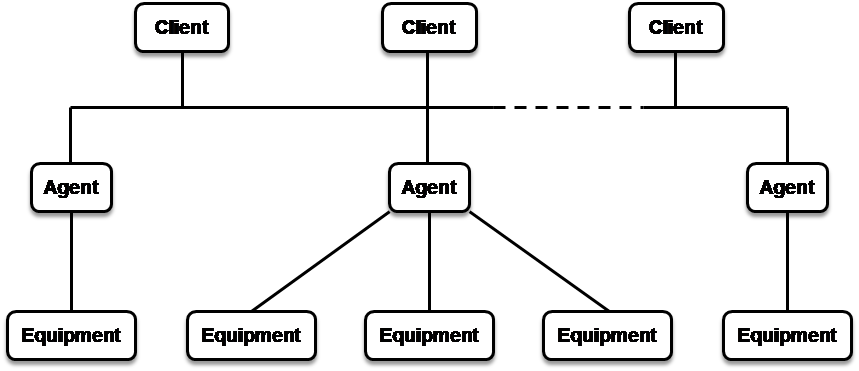
\includegraphics[width=1.0\textwidth]{figures/basic-mtconnect-implementation-structure.png}
  \caption{Basic MTConnect Implementation Structure}
  \label{fig:basic-mtconnect-implementation-structure}
\end{figure}

\FloatBarrier

The three basic modules that comprise a software system implemented using MTConnect are:

\ulheading{Equipment}:  Any data source.  In the MTConnect Standard, equipment is defined as any tangible property that is used to equip the operations of a manufacturing facility.  Examples of equipment are machine tools, ovens, sensor units, workstations, software applications, and bar feeders.

\ulheading{\gls{agent}}:  Software that collects data published from one or more piece(s) of equipment, organizes that data in a structured manner, and responds to requests for data from client software systems by providing a structured response in the form of a \gls{response document} that is constructed using the \glspl{semantic data model} defined in the Standard. 

\begin{note}
Note:	The \gls{agent} may be fully integrated into the piece of equipment or the \gls{agent} may be independent of the piece of equipment.  Implementation of an \gls{agent} is the responsibility of the supplier of the piece of equipment and/or the implementer of the \gls{agent}.
\end{note}

\ulheading{Client Software Application}:  Software that requests data from \glspl{agent} and processes that data in support of manufacturing operations. 

Based on \fig{basic-mtconnect-implementation-structure}, it is important to understand that the MTConnect Standard only addresses the following functionality and behavior of an \gls{agent}:

\begin{itemize}

\item the method used by a client software application to request information from an \gls{agent}.

\item the response that an \gls{agent} provides to a client software application.

\item a \gls{data dictionary} used to provide consistency in understanding the meaning of data reported by a data source.

\item the description of the \glspl{semantic data model} used to structure \glspl{response document} provided by an \gls{agent} to a client software application.

\end{itemize}

These functions are the primary building blocks that define the \gls{base functional structure} of the MTConnect Standard.

There are a wide variety of data sources (equipment) and data consumption systems (client software systems) used in manufacturing operations.  There are also many different uses for the data associated with a manufacturing operation.  No single approach to implementing a data communication system can address all data exchange and data management functions typically required in the data driven manufacturing environment.  MTConnect has been uniquely designed to address this diversity of data types and data usages by providing different \glspl{semantic data model} for different data application requirements:

\ulheading{Data Collection}: The most common use of data in manufacturing is the collection of data associated with the production of products and the operation of equipment that produces those products.  The MTConnect Standard provides comprehensive \glspl{semantic data model} that represent data collected from manufacturing operations.  These \glspl{semantic data model} are detailed in \citetitle{MTCPart2} and \citetitle{MTCPart3} of the MTConnect Standard.

\ulheading{Inter-operations Between Pieces of Equipment}:  The MTConnect Standard provides an \gls{interaction model} that structures the information required to allow multiple pieces of equipment to coordinate actions required to implement manufacturing activities.  This \gls{interaction model} is an implementation of a \gls{requestresponse}  messaging structure.  This \gls{interaction model} is called \gls{interfaces component} which is detailed in \citetitle{MTCPart5} of the MTConnect Standard.

\ulheading{Shared Data}:  Certain information used in a manufacturing operation is commonly shared amongst multiple pieces of equipment and/or software applications.  This information is not typically "owned" by any one manufacturing resource.  The MTConnect Standard represents this information through a series of \glspl{semantic data model} - each describing different types of information used in the manufacturing environment.  Each type of information is called an \gls{mtconnect asset}. \glspl{mtconnect asset} are detailed in \citetitle{MTCPart40}, and its \DIFdelbegin \DIFdel{sub-\textit{Parts}}\DIFdelend \DIFaddbegin \DIFadd{sub-Parts}\DIFaddend , of the MTConnect Standard.

\section{Purpose of This Document}

This document, \citetitle{MTCPart1} of the \gls{mtconnect}  Standard, addresses two major topics relating to the MTConnect Standard.  The first sections of the document define the organization of the documents used to describe the MTConnect Standard; including the terms and terminology used throughout the Standard.  The balance of the document defines the following:

\begin{itemize}
\item Operational concepts describing how an \gls{agent} should organize and structure data that has been collected from a data source.

\item Definition and structure of the \glspl{response document} supplied by an \gls{agent}.

\item The protocol used by a client software application to communicate with an \gls{agent}.
\end{itemize}

\section{Terminology and Conventions} \label{sec:Terminology and Conventions} 

\printglossary

%\printacronyms  

\printbibliography[title=MTConnect References,keyword=MTC]

%Use
%\nocite{*}
%to list all the references; used or unused

\printbibliography[title=Other References,notkeyword=MTC]

\nolinenumbers
\glsaddallunused
\nolinenumbers

\linenumbers

\section{MTConnect Standard} 
\label{mtconnect-standard}

The MTConnect Standard is organized in a series of documents (also referred to as MTConnect Documents) that each address a specific set of requirements defined by the Standard.   Each MTConnect Document will be referred to as a \DIFdelbegin \DIFdel{\textit{Part} }\DIFdelend \DIFaddbegin \DIFadd{Part }\DIFaddend of the Standard; e.g., \citetitle{MTCPart1}.  Together, these documents describe the \gls{base functional structure} specified in the MTConnect Standard.  

Implementation of any manufacturing data management system may utilize information from any number of these documents.  However, it is not necessary to realize all information contained in these documents for any one specific implementation.

\subsection{MTConnect Documents Organization}

The MTConnect specification is organized into the following documents:

\citetitle{MTCPart1}:  Provides an overview of the MTConnect Standard and defines the terminology and structure used throughout all documents associated with the Standard.  Additionally, \cite{MTCPart1} describes the functions provided by an \gls{agent} and the protocol used to communicate with an \gls{agent}.

\citetitle{MTCPart2}:  Defines the \gls{semantic data model} that describes the data that can be supplied by a piece of equipment.  This model details the \gls{xml} elements used to describe the structural and logical configuration for a piece of equipment.  It also describes each type of data that may be supplied by a piece of equipment in a manufacturing operation.

\citetitle{MTCPart3}:  Defines the \gls{semantic data model} that organizes the data that is collected from a piece of equipment and transferred to a client software application from an \gls{agent}.

\citetitle{MTCPart40}:  Provides an overview of \glspl{mtconnect asset} and the functions provided by an \gls{agent} to communicate information relating to \glspl{asset}.   The various \glspl{semantic data model} describing each type of \gls{mtconnect asset} are defined in \DIFdelbegin \DIFdel{sub-\textit{Part} documents (\textit{Part} }\DIFdelend \DIFaddbegin \DIFadd{sub-Part documents (Part }\DIFaddend 4.x) of the MTConnect Standard.

\citetitle{MTCPart5}:  Defines the MTConnect implementation of the \gls{interaction model} used to coordinate actions between pieces of equipment used in manufacturing systems.   

\subsection{MTConnect Document Versioning}

The MTConnect Standard will be periodically updated with new and expanded functionality.  Each new release of the Standard will include additional content adding new functionality and/or extensions to the \glspl{semantic data model} defined in the Standard.

The MTConnect Standard uses a three-digit version numbering system to identify each release of the Standard that indicates the progression of enhancements to the Standard.  The format used to identify the documents in a specific version of the MTConnect Standard is:

\gls{major}.\gls{minor}.\gls{revision}

\gls{major} -  Identifier representing a consistent set of functionalities defined by the MTConnect Standard. This functionality includes the protocol(s) used to communicate data to a client software application, the \glspl{semantic data model} defining how that data is organized into \glspl{response document}, and the encoding of those \glspl{response document}.  This set of functionalities is referred to as the \gls{base functional structure}.

When a release of the MTConnect Standard removes or modifies any of the protocol(s), \glspl{semantic data model}, or encoding of the \glspl{response document} included in the \gls{base functional structure} in such a way that it breaks backward compatibility and a client software application can no longer communicate with an \gls{agent} or cannot interpret the information provided by an \gls{agent}, the \gls{major} version identifier for the Documents in the release is revised to a successively higher number.

See \sect{Backwards Compatibility} for details regarding the interaction between a client software application and versions of the MTConnect Standard.

\gls{minor} - Identifier representing a specific set of functionalities defined by the MTConnect Standard.  Each release of the Standard (with a common \gls{major} version identifier) includes new and/or expanded functionality - protocol extensions, new or extended \glspl{semantic data model}, and/or new programming languages.  Each of these releases of the Standard is indicated by a successively higher \gls{minor} version identifier.   

If a new \gls{major} version of the MTConnect Standard is released, the \gls{minor} version identifier will be reset to 0.

\gls{revision} - A supplemental identifier representing only organizational or editorial changes to a \gls{minor} version document with no changes in the functionality described in that document.

New releases of a specific document are indicated by a successively higher revision version identifier.

If a new \gls{minor} version of a document is released, the \gls{revision} identifier will be reset to 0.

An example of the version identifier for a specific document would be: 

\centerline{Version M.N.R}

\subsubsection{Document Releases}

A \gls{major} revision change represents a substantial change to the MTConnect Standard.  At the time of a \gls{major} revision change, all documents representing the MTConnect Standard will be updated and released together.

A \gls{minor} revision change represents some level of extended functionality supported by the MTConnect Standard.  At the time of a \gls{minor} version release, MTConnect Documents representing the changes or enhancements to the Standard will be updated as required. However, all documents, whether updated or not, will be released together with a new \gls{minor} version number.  Providing all documents at a common \gls{major} and \gls{minor} version makes it easier for implementers to manage the compatibility and upgrade of the different software tools incorporated into a manufacturing software system.

Since a \gls{revision} represents no functional changes to the MTConnect Standard and includes only editorial or descriptive changes that enhance the understanding of the functionality supported by the Standard, individual documents within the Standard may be released at any time with a new \gls{revision} and that release does not impact any other documents associated with the MTConnect Standard.

The latest released version of each document provided for the MTConnect Standard, and historical releases of those documents, are provided at http://www.mtconnect.org.

\newpage

\subsection{MTConnect Document Naming Conventions}

MTConnect Documents are identified as follows:

\subsubsection{Document Title}

Each MTConnect Document \MUST be identified as follows:

\newline \centerline{\large{\textbf{\mtconnectregistered Standard}}}
\newline \centerline{Part \#.\# - \textit{Title}}
\newline \centerline{Version M.N.R.}

The following keys are used to distinguish different \DIFdelbegin \DIFdel{\textit{Parts} }\DIFdelend \DIFaddbegin \DIFadd{Parts }\DIFaddend of the MTConnect Standard and the version of the MTConnect Document:

\tab	\#.\# - Identifier of the specific Part and \DIFdelbegin \DIFdel{sub-\textit{Part} }\DIFdelend \DIFaddbegin \DIFadd{sub-Part }\DIFaddend of the MTConnect Standard 

\tab	Title - Description of the type of information contained in the MTConnect Document

\tab	M - Indicator of the \gls{major} version of the MTConnect Document

\tab	N- Indicator of the \gls{minor} version of the MTConnect Document

\tab	R - Indicator of the revision of the MTConnect Document

For example, a release of \citetitle{MTCPart2} would be:

\newline \centerline{\large{\textbf{\mtconnectregistered Standard}}}
\newline \centerline{Part 2.0 - \textit{\glspl{device information model}}}
\newline \centerline{Version 1.2.0}

\subsubsection{Electronic Document File Naming}

Electronic versions of the MTConnect Documents will be provided in PDF format and follow this naming convention:

\tab MTC\_Part\#-\#\_Title\_M-N-R.pdf 

The electronic version of the same release of \citetitle{MTCPart2} would be:

\tab MTC\_Part\_2-0\_Devices\_Information\_Model\_1-2-0.pdf

\subsection{Document Conventions}

Additional information regarding specific content in the MTConnect Standard is provided in the sections below.

\subsubsection{Use of MUST, SHOULD, and MAY}

These words convey specific meaning in the MTConnect Standard when presented in capital letters, Times New Roman font, and a Bold font style. 

\begin{itemize}
\item	The word \MUST indicates content that is mandatory to be provided in an implementation where indicated.

\item	The word \SHOULD indicates content that is recommended, but the exclusion of which will not invalidate an implementation.

\item	The word \MAY indicates content that is optional.  It is up to the implementer to decide if the content is relevant to an implementation.

\item 	The word \NOT may be added to the words \MUST or \SHOULD to negate the requirement.
\end{itemize}

\subsubsection{Text Conventions}

The following conventions will be used throughout the MTConnect Documents to provide a clear and consistent understanding of the use of each type of information used to define the MTConnect Standard.

These conventions are:

\begin{itemize}
\item	Standard text is provided in Times New Roman font.

\item	References to documents, sections or sub-sections of a document, or figures within a document are \textit{italicized}; e.g., \citetitle{MTCPart2}.

\item 	Terms with a specific meaning in the MTConnect Standard will be \textit{italicized}; e.g., \gls{major} indicating a version of the Standard.

\item 	When these same terms are used within the text without specific reference to their function within the MTConnect Standard, they will be provided as non-italicized font; e.g., major indicating a descriptor of another term.

\item 	Terms representing content of an MTConnect \gls{semantic data model} or the protocol used in MTConnect will be provided in fixed size, Courier New font; e.g., \gls{component componentstream}, \gls{probe httprequest}, \gls{current httprequest}.   

\tab When these same terms are used within the text without specific reference to their function within the MTConnect Standard, they will be provided as Times New Roman font.

\item	All \glspl{valid data value} that are restricted to a limited or controlled vocabulary will be provided in upper case Courier New font with an \textunderscore  (underscore) separating words.  For example: \gls{on value}, \gls{off value}, \gls{actual subtype}, \gls{counterclockwise value}, etc.

\item 	All descriptive attributes associated with each piece of data defined in a \gls{response document} will be provided in Courier New font and camel case font style.  For example: \gls{nativeunits}.
\end{itemize}

\subsubsection{Code Line Syntax and Conventions}

The following conventions will be used throughout the MTConnect Documents to describe examples of software code produced by an \gls{agent} or commands provided to an \gls{agent} from a client software application.

All examples are provided in fixed size Courier New font with line numbers.

These conventions are:

\begin{itemize}

\item \gls{xml} Code examples:

\begin{lstlisting}[firstnumber=last,escapechar=|,%
    caption={XML Code Examples},label={lst:xml-code-examples}]
<MTConnectStreams xmlns:m="urn:mtconnect.com:
    MTConnectStreams:1.1" xmlns:xsi=
    "http://www.w3.org/2001/XMLSchema-instance"
    xmlns="urn:mtconnect.com:MTConnectStreams:1.1"
\end{lstlisting}

\item HTTP URL examples:

\begin{itemize}

\item	http://<authority>/<path>[?<query>]When a portion of a URL is enclosed in angle brackets ("<" and ">"), that section of the URL is a place holder for specific information that will replace the term between the angle brackets. 

\begin{note}
Note:  The angle brackets in a URL do not relate to the angle brackets used as the \cfont{tag} elements in an \gls{xml} example.

\end{note}

\item A portion of a URL that is enclosed in square brackets "[" and "]" indicates that the enclosed content is optional. 

\item All other characters in the URL are literal.

\end{itemize}

\end{itemize}

\subsubsection{Semantic Data Model Content}

For each of the \glspl{semantic data model} defined in the MTConnect Standard, there are tables describing pieces of information provided in the data models.  Each table has a column labeled \gls{occurrence}. \gls{occurrence} defines the number of times the content defined in the tables \MAY be provided in the usage case specified.

\begin{itemize}

\item If the \gls{occurrence} is 1, the content \MUST be provided.

\item If the \gls{occurrence} is 0..1, the content \MAY be provided and if provided, at most, only one occurrence of the content \MUST be provided.

\item If the \gls{occurrence} is 0..*, the content \MAY be provided and any number of occurrences of the content \MAY be provided.

\item If the \gls{occurrence} is 1..*, one or more occurrences of the content \MUST be provided.

\item If the \gls{occurrence} is a number, e.g., 2, exactly that number of occurrences of the content \MUST be provided.

\end{itemize}

\begin{note}
Note: "*" indicates multiple number of occurrences and is represented by $\infty$ in the figures.

\end{note}

\subsubsection{Referenced Standards and Specifications}

Other standards and specifications may be used to describe aspects of the protocol, \gls{data dictionary}, or \glspl{semantic data model} defined in the MTConnect Standard.  When a specific standard or specification is referenced in the MTConnect Standard, the name of the standard or specification will be provided in \textit{italicized} font.  

See \sect{Terminology and Conventions}:  Bibliography for a complete listing of standards and specifications used or referenced in the MTConnect Standard. 

\subsubsection{Deprecation and Deprecation Warnings}

When the MTConnect Institute adds new functionality to the MTConnect Standard, the new content may supersede some of the functionality of existing content or significantly enhance one of the \glspl{semantic data model}.  When this occurs, existing content may no longer be valid for use in the new version of the Standard.

\paragraph{Deprecation}\mbox{}

In cases when new content supersedes the functionality of the existing content, the original content \MUST no longer be included in future implementations - only the new content should be used.

The superseded content is identified by striking through the original content (\deprecated{original content}) and marking the content with the words "\DEPRECATED in \textit{Version M.N}".

The deprecated content must remain in all future \gls{minor} versions of the document.  The content may be removed when a \gls{major} version update is released.  This provides implementers guidance on how to interpret data that may be provided from equipment utilizing an older version of the Standard.  This content provides the information required for implementers to develop software applications that support backwards compatibility with older versions of the standard.

A software application may be designed to be compliant with any specific \gls{minor} version of the standard.  That software application may be collecting data from many different pieces of equipment.  Each of these pieces of equipment may be providing data defined by the current version or any of the previous \gls{minor} versions of the standard.  To maintain compatibility with existing pieces of equipment, software applications should be implemented to interpret data defined in the current release of the MTConnect Standard, as well as all deprecated content associated with earlier versions of the Standard.

\paragraph{Deprecation Warning}\mbox{}

When new content provides improved alternatives for defining the \glspl{semantic data model}, the MTConnect Institute may determine that the original content could possibly be deprecated in the future.  When this occurs, a content will be marked with the words "\DEPRECATIONWARNING" to identify the content that may be deprecated in the future.  This provides advanced notice to implementers that they should choose to utilize the improved alternatives when developing new products or software systems to avoid the possibility that the original content may be deprecated in a future version of the Standard. 

%\subsection{Document Version Management} 

\subsection{Backwards Compatibility}
\label{sec:Backwards Compatibility}

MTConnect Documents with a different \gls{major} version identifier represent a significant change in the \gls{base functional structure} of the MTConnect Standard.  This means that the schema or protocol defined by the Standard may have changed in ways that will require software applications to change how they request and/or interpret data received from an \gls{agent}.  Software applications should be fully version aware since no assumption of backwards compatibility should be assumed at the time of a \gls{major} revision change to the MTConnect Standard.

The MTConnect Institute strives to maintain version compatibility through all \gls{minor} revisions of the MTConnect Standard.  New \gls{minor} versions may introduce extensions to existing \glspl{semantic data model}, extend the protocol used to communicate to the \gls{agent}, and/or add new \glspl{semantic data model} to extend the functionality of the Standard.  Client software applications may be designed to be compliant with any specific \gls{minor} version of the MTConnect Standard.  Additionally, software applications should be capable of interpreting information from an \gls{agent} providing data based upon a lower \gls{minor} version identifier.  It should also be capable of interpreting information from an \gls{agent} providing data based upon a higher \gls{minor} version identifier of the MTConnect Standard than the version supported by the client, even though the client may ignore or not be capable of interpreting the extended content provided by the \gls{agent}.

A \gls{revision} version of any MTConnect Document provides only editorial changes requiring no changes to an \gls{agent} or a client application.

\section{MTConnect Fundamentals}

The MTConnect Standard defines the functionality of an \gls{agent}.  In an MTConnect installation, pieces of equipment publish information to an \gls{agent}.  Client software applications request information from the \gls{agent} using a communications protocol.  Based on the specific information that the client software application has requested from the \gls{agent}, the \gls{agent} forms a \gls{response document} based upon one of the \glspl{semantic data model} defined in the MTConnect Standard and then transmits that document to the client software application.  

\fig{mtconnect-architecture-model} illustrates the architecture of a typical MTConnect installation. 

\begin{figure}[ht]
  \centering
  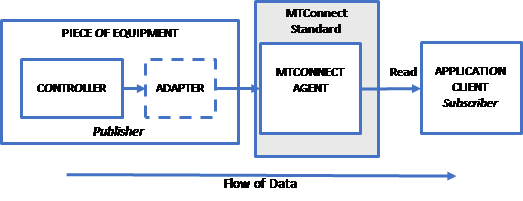
\includegraphics[width=1.0\textwidth]{figures/mtconnect-architecture-model.png}
  \caption{MTConnect Architecture Model}
  \label{fig:mtconnect-architecture-model}
\end{figure}

\FloatBarrier

\begin{note}
Note: In each implementation of a communication system based on the MTConnect Standard, there \MUST be a schema defined that encodes the rules and terminology defined for each of the \glspl{semantic data model}.  These schemas \MAY be used by client software applications to validate the content and structure of the \glspl{response document} published by an \gls{agent}.

\end{note}

\subsection{Agent}

An \gls{agent} is the centerpiece of an MTConnect implementation.  It provides two primary functions:

\begin{itemize}

\item Organizes and manages individual pieces of information published by one or more pieces of equipment.

\item Publishes that information in the form of a \gls{response document} to client software applications.

\end{itemize}

The MTConnect Standard addresses the behavior of an \gls{agent} and the structure and meaning of the data published by an \gls{agent}.  It is the responsibility of the implementer of an \gls{agent} to determine the means by which the behavior is achieved for a specific \gls{agent}.

An \gls{agent} is software that may be installed as part of a piece of equipment or it may be installed separately.  When installed separately, an \gls{agent} may receive information from one or more pieces of equipment.

Some pieces of equipment may be able to communicate directly to an \gls{agent}.  Other pieces of equipment may require an \gls{adapter} to transform the information provided by the equipment into a form that can be sent to an \gls{agent}.  In either case, the method of transmitting information from the piece of equipment to an \gls{agent} is implementation dependent and is not addressed as part of the MTConnect Standard.

One function of an \gls{agent} is to store information that it receives from a piece of equipment in an organized manner.  A second function of an \gls{agent} is to receive \glspl{request} for information from one or many client software applications and then respond to those \glspl{request} by publishing a \gls{response document} that contains the requested information.

There are three types of information stored by an \gls{agent} that \MAY be published in a \gls{response document}.  These are:

\begin{itemize}

\item \gls{equipment metadata} defines the \glspl{structural element} that represent the physical and logical parts and sub-parts of each piece of equipment that can publish data to the \gls{agent}, the relationships between those parts and sub-parts, and the \glspl{data entity} associated with each of those \glspl{structural element}.  This \gls{equipment metadata} is provided in an \gls{mtconnectdevices response document}. See \citetitle{MTCPart2} for more information on \gls{equipment metadata}.

\item \gls{streaming data} provides the values published by pieces of equipment for the \glspl{data entity} defined by the \gls{equipment metadata}.  \gls{streaming data} is provided in an \gls{mtconnectstreams response document}.  See \citetitle{MTCPart2} for more information on \gls{streaming data}.

\item \glspl{mtconnect asset} represent information used in a manufacturing operation that is commonly shared amongst multiple pieces of equipment and/or software applications.  \glspl{mtconnect asset} are provided in an \gls{mtconnectassets response document}.  See \citetitle{MTCPart40} for more information on \glspl{mtconnect asset}.

\end{itemize}

The exchange between an \gls{agent} and a client software application is a \gls{request} and \gls{response} information exchange mechanism.  See \sect{Request/Response Information Exchange} for details on this \gls{requestresponse} information exchange mechanism.

\subsubsection{Instance of an Agent}
\label{sec:Instance of an Agent}

As described above, an \gls{agent} collects and organizes values published by pieces of equipment.  As with any piece of software, an \gls{agent} may be periodically restarted.  When an \gls{agent} restarts, it \MUST indicate to client software applications whether the information available in the \gls{buffer} represents a completely new set of data or if the \gls{buffer} includes data that had been collected prior to the restart of the \gls{agent}.

Any time an \gls{agent} is restarted and begins to collect a completely new set of \gls{streaming data}, that set of data is referred to as an \gls{instance} of the \gls{agent}.  The \gls{agent} \MUST maintain a piece of information called \gls{instanceid} that represents the specific \gls{instance} of the \gls{agent}.

\gls{instanceid} is represented by a 64-bit integer.  The \gls{instanceid} \MAY be implemented using any mechanism that will guarantee that the value for \gls{instanceid} will be unique each time the \gls{agent} begins collecting a new set of data.

When an \gls{agent} is restarted and it provides a method to recover all, or some portion, of the data that was stored in the \gls{buffer} before it stopped operating, the \gls{agent} \MUST use the same \gls{instanceid} that was defined prior to the restart. 

\subsubsection{Storage of Equipment Metadata for a Piece of Equipment}

An \gls{agent} \MUST be capable of publishing \gls{equipment metadata} for each piece of equipment that publishes information through the \gls{agent}.  \gls{equipment metadata} is typically a static file defining the \glspl{structural element} associated with each piece of equipment reporting information through the \gls{agent} and the \glspl{data entity} that can be associated with each of these \glspl{structural element}.  See details on \glspl{structural element} and \glspl{data entity} in \citetitle{MTCPart2}.

The MTConnect Standard does not define the mechanism to be used by an \gls{agent} to acquire, maintain, or store the \gls{equipment metadata}.  This mechanism \MUST be defined as part of the implementation of a specific \gls{agent}.

\subsubsection{Storage of Streaming Data}

\gls{streaming data} that is published from a piece(s) of equipment to an \gls{agent} is stored by the \gls{agent} based upon the sequence upon which each piece of data is received.  As described below, the order in which data is stored by the \gls{agent} is one of the factors that determines the data that may be included in a specific \gls{mtconnectstreams response document}. 

\paragraph{Management of Streaming Data Storage}\mbox{}
\label{sec:Management of Streaming Data Storage}

An \gls{agent} stores a fixed amount of data.  The amount of data stored by an \gls{agent} is dependent upon the implementation of a specific \gls{agent}.  The examples below demonstrate how discrete pieces of data received from pieces of equipment are stored.

The method for storing \gls{streaming data} in an \gls{agent} can be thought of as a tube that can hold a finite set of balls.  Each ball represents the occurrence of a \gls{data entity} published by a piece of equipment.  This data is pushed in one end of the tube until there is no more room for additional balls.  At that point, any new data inserted will push the oldest data out the back of the tube.  The data in the tube will continue to shift in this manner as new data is received.

This tube is referred to as a \gls{buffer} in an \gls{agent}.

\begin{figure}[ht]
  \centering
  
\includegraphics[width=1.0\textwidth]{figures/data-storage-in-buffer.png}
  \caption{Data Storage in Buffer}
  \label{fig:data-storage-in-buffer}
\end{figure}

\FloatBarrier

In \fig{first-in-first-out-buffer-management}, the maximum number of \glspl{data entity} that can be stored in the \gls{buffer} of the \gls{agent} is 8.  The maximum number of \glspl{data entity} that can be stored in the \gls{buffer} is represented by a value called \gls{buffersize}.  This example illustrates that when the \gls{buffer} fills up, the oldest piece of data falls out the other end.

\begin{figure}[ht]
  \centering
  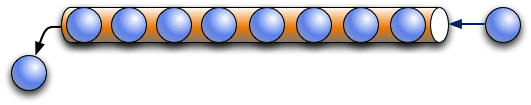
\includegraphics[width=1.0\textwidth]{figures/first-in-first-out-buffer-management.png}
  \caption{First In First Out Buffer Management}
  \label{fig:first-in-first-out-buffer-management}
\end{figure}

\FloatBarrier

This process constrains the memory storage requirements for an \gls{agent} to a fixed maximum size since the MTConnect Standard only requires an \gls{agent} to store a finite number of pieces of data.

As an implementation guideline, the \gls{buffer} \SHOULD be sized large enough to provide storage for a reasonable amount of information received from all pieces of equipment that are publishing information to that \gls{agent}.  The implementer should also consider the impact of a temporary loss of communications between a client software application and an \gls{agent} when determining the size for the \gls{buffer}.  A larger \gls{buffer} will allow a client software application more time to reconnect to an \gls{agent} without losing data.

\paragraph{Sequence Numbers}\mbox{}

In an \gls{agent}, each occurrence of a \gls{data entity} in the \gls{buffer} will be assigned a monotonically increasing \gls{sequence number} as it is inserted into the \gls{buffer}.  The \gls{sequence number} is a 64-bit integer and the values assigned as \glspl{sequence number} will never wrap around or be exhausted; at least within the next 100,000 years based on the size of a 64-bit number.

\gls{sequence number} is the primary key identifier used to manage and locate a specific piece of data in an \gls{agent}.  The \gls{sequence number} associated with each \gls{data entity} reported by an \gls{agent} is identified with an attribute called \gls{sequence}.

The \gls{sequence number} for each piece of data \MUST be unique for an instance of an \gls{agent} (see \sect{Instance of an Agent} for information on \glspl{instance} of an \gls{agent}).  If data is received from more than one piece of equipment, the \glspl{sequence number} are based on the order in which the data is received regardless of which piece of equipment produced that data.  The \gls{sequence number} \MUST be a monotonically increasing number that spans all pieces of equipment publishing data to an \gls{agent}.  This allows for multiple pieces of equipment to publish data through a single \gls{agent} with no \gls{sequence number} collisions and unnecessary protocol complexity.

The \gls{sequence number} \MUST be reset to one (1) each time an \gls{agent} is restarted and begins to collect a fresh set of data; i.e., each time \gls{instanceid} is changed.

\fig{instanceid-and-sequence} demonstrates the relationship between \gls{instanceid} and sequence when an \gls{agent} stops and restarts and begins collecting a new set of data.  In this case, the \gls{instanceid} is changed to a new value and value for \gls{sequence} resets to one (1):

\begin{figure}[ht]
  \centering
  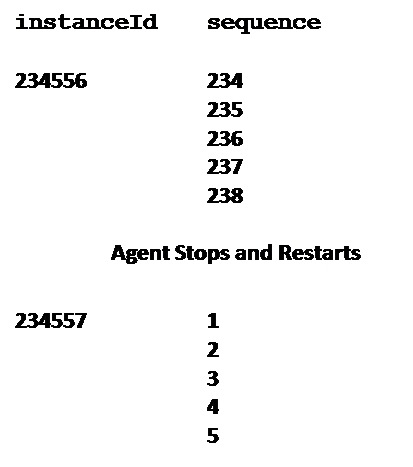
\includegraphics[width=0.5\textwidth]{figures/instanceid-and-sequence.png}
  \caption{instanceId and sequence}
  \label{fig:instanceid-and-sequence}
\end{figure}

\FloatBarrier


\fig{identifying-the-range-of-data-with-firstsequence-and-lastsequence} also shows two additional pieces of information defined for an \gls{agent}:

\begin{itemize}
\item \gls{firstsequence} - the oldest piece of data contained in the \gls{buffer}; i.e., the next piece of data to be moved out of the \gls{buffer}

\item \gls{lastsequence} - the newest data added to the \gls{buffer}
\end{itemize}

\gls{firstsequence} and \gls{lastsequence} provide guidance to a software application identifying the range of data available that may be requested from an \gls{agent}. 

\begin{figure}[ht]
  \centering
  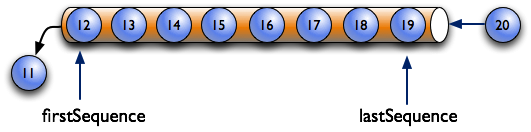
\includegraphics[width=1.0\textwidth]{figures/identifying-the-range-of-data-with-firstsequence-and-lastsequence.png}
  \caption{Indentifying the range of data with firstSequence and lastSequence}
  \label{fig:identifying-the-range-of-data-with-firstsequence-and-lastsequence}
\end{figure}

\FloatBarrier

When a client software application requests data from an \gls{agent}, it can specify both the \gls{sequence number} of the first piece of data (\gls{from query}) that \MUST be included in the \gls{response document} and the total number (\gls{count model}) of pieces of data that \SHOULD be included in that document.

In \fig{identifying-the-range-of-data-with-from-and-count}, the request specifies that the data to be returned starts at \gls{sequence number} 15 (\gls{from query}) and includes a total of three items (\gls{count model}).  

\begin{figure}[ht]
  \centering
  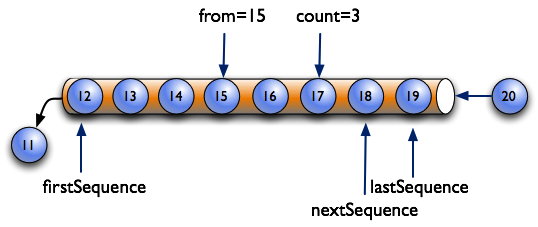
\includegraphics[width=1.0\textwidth]{figures/identifying-the-range-of-data-with-from-and-count.png}
  \caption{Identifying the range of data with from and count}
  \label{fig:identifying-the-range-of-data-with-from-and-count}
\end{figure}

\FloatBarrier


Once a \gls{response} to a \gls{request} has been completed, the value of \gls{nextsequence} will be established.  \gls{nextsequence} is the \gls{sequence number} of the next piece of data available in the \gls{buffer}.  In the example in \fig{identifying-the-range-of-data-with-from-and-count}, the next \gls{sequence number} (\gls{nextsequence}) will be 18.

As shown in \fig{identifying-the-range-of-data-with-nextsequence-and-lastsequence}, the combination of \gls{from query} and \gls{count model} defined by the \gls{request} indicates a \gls{sequence number} for data that is beyond that which is currently in the \gls{buffer}.  In this case, \gls{nextsequence} is set to a value of \gls{lastsequence} + 1.  

\begin{figure}[ht]
  \centering
  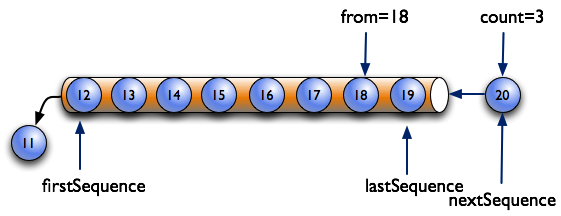
\includegraphics[width=1.0\textwidth]{figures/identifying-the-range-of-data-with-nextsequence-and-lastsequence.png}
  \caption{Indentifying the range of data with nextSequence and lastSequence}
  \label{fig:identifying-the-range-of-data-with-nextsequence-and-lastsequence}
\end{figure}

\FloatBarrier

\paragraph{Buffer Data Structure}\mbox{}

The information in the \gls{buffer} of an \gls{agent} can be thought of as a four-column table of data.  Each column in the table represents:

\begin{itemize}
\item The first column is the \gls{sequence number} associated with each \gls{data entity} - \gls{sequence}.

\item The second column is the time that the data was published by a piece of equipment.  This time is defined as the \gls{timestamp} associated with that \gls{data entity}.  See \sect{Time Stamp} for details on \gls{timestamp}.

\item The third column, \gls{dataitemid}, refers to the identity of \glspl{data entity} as they will appear in the \gls{mtconnectstreams response document}.  See \textit{Section 5} of \citetitle{MTCPart3} for details on \gls{dataitemid} for a \gls{data entity} and how that identify relates to the \gls{id} attribute of the corresponding \gls{data entity} in the \glspl{device information model}.

\item The fourth column is the value associated with each \gls{data entity}.
\end{itemize}

\fig{data-storage-concept} is an example demonstrating the concept of how data may be stored in an \gls{agent}:

\begin{figure}[ht]
  \centering
  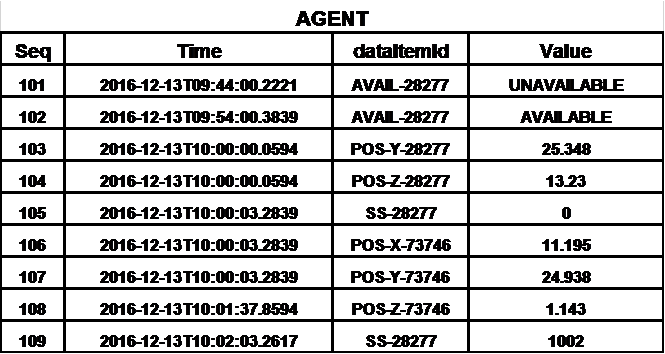
\includegraphics[width=1.0\textwidth]{figures/data-storage-concept.png}
  \caption{Data Storage Concept}
  \label{fig:data-storage-concept}
\end{figure}

\FloatBarrier


The storage mechanism for the data, the internal representation of the data, and the implementation of the \gls{agent} itself is not part of the MTConnect Standard.  The implementer can choose both the amount of data to be stored in the \gls{agent} and the mechanism for how the data is stored.  The only requirement is that an \gls{agent} publish the \glspl{response document} in the required format.  

\paragraph{Time Stamp}\mbox{}
\label{sec:Time Stamp}

Each piece of equipment that publishes information to an \gls{agent} \SHOULD provide a time stamp indicating when each piece of information was measured or determined.  If no time stamp is provided, the \gls{agent} \MUST provide a time stamp for the information based upon when that information was received at the \gls{agent}.

The \gls{timestamp} associated with each piece of information is reported by an \gls{agent} as \gls{timestamp}.  \gls{timestamp} \MUST be reported in UTC (Coordinated Universal Time) format; e.g., "2010-04-01T21:22:43Z".

\begin{note}
Note:  Z refers to UTC/GMT time, not local time.

\end{note}

Client software applications should use the value of \gls{timestamp} reported for each piece of information as the means for ordering when pieces of information were generated as opposed to using \gls{sequence} for this purpose.

\begin{note}
Note: It is assumed that \gls{timestamp} provides the best available estimate of the time that the value(s) for the published information was measured or determined.

\end{note}

If two pieces of information are measured or determined at the exact same time, they \MUST be reported with the same value for \gls{timestamp}.  Likewise, all information that is recorded in the \gls{buffer} with the same value for \gls{timestamp} should be interpreted as having been recorded at the same point in time; even if that data was published by more than one piece of equipment. 

\paragraph{Recording Occurrences of Streaming Data}\mbox{}

An \gls{agent} \MUST record data in the \gls{buffer} each time the value for that specific piece of data changes.  If a piece of equipment publishes multiple occurrences of a piece of data with the same value, the \gls{agent} \MUSTNOT record multiple occurrence for that \gls{data entity}.

\begin{note}
Note:	There is one exception to this rule.  Some \glspl{data entity} may be defined with a \gls{representation} attribute value of \gls{discrete representation} (See \textit{Section 7.2.2.12} of \citetitle{MTCPart2} for details on \gls{representation}.)  In this case, each occurrence of the data represents a new and unique piece of information.  The \gls{agent} \MUST then record each occurrence of the \gls{data entity} that is published by a piece of equipment.

\end{note}

The value for each piece of information reported by an \gls{agent} must be considered by a client software application to be valid until such a time that another occurrence of that piece of information is published by the \gls{agent}.

\paragraph{Maintaining Last Value for Data Entities}\mbox{}

An \gls{agent} \MUST retain a copy of the last available value associated with each \gls{data entity} known to the \gls{agent}; even if an occurrence of that \gls{data entity} is no longer in the \gls{buffer}.  This function allows an \gls{agent} to provide a software application a view of the last known value for each \gls{data entity} associated with a piece of equipment.

The \gls{agent} \MUST also retain a copy of the last value associated with each \gls{data entity} that has flowed out of the \gls{buffer}.  This function allows an \gls{agent} to provide a software application a view of the last known value for each \gls{data entity} associated with a \gls{current request} with an \gls{at query} parameter in the \gls{query http request} portion of its \gls{http request line} (See \sect{Current Request Implemented Using HTTP} for details on \gls{current request}).

\newpage

\paragraph{Unavailability of Data}\mbox{}

An \gls{agent} \MUST maintain a list of \glspl{data entity} that \MAY be published by each piece of equipment providing information to the \gls{agent}.   This list of \glspl{data entity} is derived from the \gls{equipment metadata} stored in the \gls{agent} for each piece of equipment.

Each time an \gls{agent} is restarted, the \gls{agent} \MUST place an occurrence of every \gls{data entity} in the \gls{buffer}.  The value reported for each of these \glspl{data entity} \MUST be set to \gls{unavailable value} and the \gls{timestamp} for each \MUST be set to the time that the last piece of data was collected by the \gls{agent} prior to the restart.

If at any time an \gls{agent} loses communications with a piece of equipment, or the \gls{agent} is unable to determine a valid value for all, or any portion, of the \glspl{data entity} published by a piece of equipment, the \gls{agent} \MUST place an occurrence of each of these \glspl{data entity} in the \gls{buffer} with its value set to \gls{unavailable value}.  This signifies that the value is currently indeterminate and no assumptions of a valid value for the data is possible.

Since an \gls{agent} may receive information from multiple pieces of equipment, it \MUST consider the validity of the data from each of these pieces of equipment independently.

There is one exception to the rules above.  Any \gls{data entity} that is constrained to a constant data value \MUST be reported with the constant value and the \gls{agent} \MUSTNOT set the value of that \gls{data entity} to \gls{unavailable value}.

\begin{note}
Note:	The schema for the \glspl{device information model} (defined in \citetitle{MTCPart2}) defines how the value reported for an individual piece of data may be constrained to one or more specific values.

\end{note}

\paragraph{Persistence and Recovery}\mbox{}

The implementer of an \gls{agent} must decide on a strategy regarding the storage of \gls{streaming data} in the \gls{buffer} of the \gls{agent}.

In the simplest form, an \gls{agent} can hold the \gls{buffer} information in volatile memory where no data is persisted when the \gls{agent} is stopped.  In this case, the \gls{agent} \MUST update the value for \gls{instanceid} when the \gls{agent} restarts to indicate that the \gls{agent} has begun to collect a new set of data.

If the implementation of an \gls{agent} provides a method of persisting and restoring all or a portion of the information in the \gls{buffer} of the \gls{agent} (\glspl{sequence number}, \glspl{time stamp}, identify, and values), the \gls{agent} \MUSTNOT change the value of the \gls{instanceid} when the \gls{agent} restarts.  This will indicate to a client software application that it does not need to reset the value for \gls{nextsequence} when it requests the next set of data from the \gls{agent}.

When an implementer chooses to provide a method to persist the information in an \gls{agent}, they may choose to store as much data as is practical in a recoverable storage system.  Such a method may also include the ability to store historical information that has previously been pushed out of the \gls{buffer}.

\paragraph{Heartbeat}\mbox{}

An \gls{agent} \MUST provide a function that indicates to a client application that the HTTP connection is still viable during times when there is no new data available to report in a \gls{response document}.  This function is defined as \gls{heartbeat}.

\gls{heartbeat} represents the amount of time after a \gls{response document} has been published until a new \gls{response document} \MUST be published, even when no new data is available.

See \sect{Query Portion of the HTTP Request Line for a Sample Request} for more details on configuring the \gls{heartbeat} function.

\paragraph{Data Sets}\mbox{}
\label{sec:Data Sets}

See \citetitle{MTCPart3} \textit{Section Part 3: DataItem with representation of DATA\textunderscore SET} for management of \glspl{data set}.


\subsubsection{Storage of Documents for MTConnect Assets}

An \gls{agent} also stores information associated with \glspl{mtconnect asset}.

When a piece of equipment publishes a document that represents information associated with an \gls{mtconnect asset}, an \gls{agent} stores that document in a \gls{buffer}.  This \gls{buffer} is called the \glspl{asset buffer}.  The document is called an \gls{asset document}.

The \glspl{asset buffer} \MUST be a separate \gls{buffer} from the one where the \gls{streaming data} is stored.

The \gls{asset document} that is published by the piece of equipment \MUST be organized based upon one of the applicable \glspl{asset information model} defined in one of the \DIFdelbegin \DIFdel{\textit{Parts} }\DIFdelend \DIFaddbegin \DIFadd{Parts }\DIFaddend 4.x of the MTConnect Standard.

An \gls{agent} will only retain a limited number of \glspl{asset document} in the \glspl{asset buffer}.  The \glspl{asset buffer} functions similar to the \gls{buffer} for \gls{streaming data}; i.e., when the \glspl{asset buffer} is full, the oldest \gls{asset document} is pushed from the \gls{buffer}.

\fig{first-in-first-out-asset-buffer-management} demonstrates the oldest \gls{asset document} being pushed from the \glspl{asset buffer} when a new \gls{asset document} is added and the \glspl{asset buffer} is full:

\begin{figure}[ht]
  \centering
  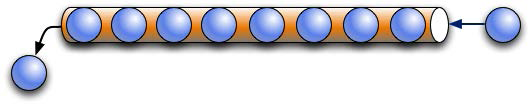
\includegraphics[width=1.0\textwidth]{figures/first-in-first-out-asset-buffer-management.png}
  \caption{First In First Out Asset Buffer Management}
  \label{fig:first-in-first-out-asset-buffer-management}
\end{figure}

\FloatBarrier

Within an \gls{agent}, the management of \glspl{asset document} behave like a key/value storage in a database.  In the case of \glspl{mtconnect asset}, the key is an identifier for an Asset (see details on \gls{assetid} in \citetitle{MTCPart40}) and the value is the \gls{asset document} that was published by the piece of equipment. 

\fig{relationship-between-assetid-and-stored-asset-documents} demonstrates the relationship between the key (\gls{assetid}) and the stored \glspl{asset document}:

\begin{figure}[ht]
  \centering
  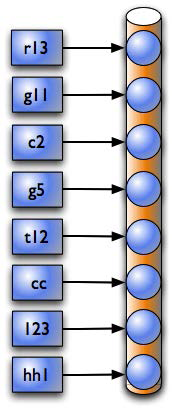
\includegraphics[width=0.3\textwidth]{figures/relationship-between-assetid-and-stored-asset-documents.png}
  \caption{Relationship between assetId and stored Asset documents}
  \label{fig:relationship-between-assetid-and-stored-asset-documents}
\end{figure}

\FloatBarrier

\begin{note}
Note:  The key (\gls{assetid}) is independent of the order of the \glspl{asset document} stored in the \glspl{asset buffer}.

\end{note}

When an \gls{agent} receives a new \gls{asset document} representing an \gls{mtconnect asset}, it must determine whether this document represents an \gls{mtconnect asset} that is not currently represented in the \glspl{asset buffer} or if the document represents new information for an \gls{mtconnect asset} that is already represented in the \glspl{asset buffer}.  When a new \gls{asset document} is received, one of the following \MUST occur:

\begin{itemize}

\item If the \gls{asset document} represents an \gls{mtconnect asset} that is not currently represented in the \glspl{asset buffer}, the \gls{agent} \MUST add the new document to the front of the \glspl{asset buffer}.  If the \glspl{asset buffer} is full, the oldest \gls{asset document} will be removed from the \glspl{asset buffer}.

\item If the \gls{asset document} represents an \gls{mtconnect asset} that is already represented in the \glspl{asset buffer}, the \gls{agent} \MUST remove the existing \gls{asset document} representing that \gls{mtconnect asset} from the \glspl{asset buffer} and add the new \gls{asset document} to the front of the \glspl{asset buffer}.  

\end{itemize}

The MTConnect Standard does not specify the maximum number of \glspl{asset document} that may be stored in the \glspl{asset buffer}; that limit is determined by the implementation of a specific \gls{agent}.  The number of \glspl{asset document} that may be stored in an \gls{agent} is defined by the value for \gls{assetbuffersize} (See \sect{Document Header} for more information on \gls{assetbuffersize}.).  A value of 4,294,967,296 or $2^{32}$ can be provided for \gls{assetbuffersize} to indicate unlimited storage.

There is no requirement for an \gls{agent} to provide persistence for the \glspl{asset document} stored in the \glspl{asset buffer}.  If an \gls{agent} should fail, all \glspl{asset document} stored in the \glspl{asset buffer} \MAY be lost.  It is the responsibility of the implementer to determine if \glspl{asset document} stored in an \gls{agent} may be restored or if those \glspl{asset document} are retained by some other software application.

Additional details on how an \gls{agent} organizes and manages information associated with \glspl{mtconnect asset} are provided in \citetitle{MTCPart40}. 

\subsection{Response Documents}

\glspl{response document} are electronic documents generated and published by an \gls{agent} in response to a \gls{request} for data. 

The \glspl{response document} defined in the MTConnect Standard are:

\begin{itemize}

\item \gls{mtconnectdevices response document}:  An electronic document that contains the information published by an \gls{agent} describing the data that can be published by one or more piece(s) of equipment.  The structure of the \gls{mtconnectdevices response document} document is based upon the requirements defined by the \glspl{device information model}.  See \citetitle{MTCPart2} for details on this information model.

\item \gls{mtconnectstreams response document}:  An electronic document that contains the information published by an \gls{agent} that contains the data that is published by one or more piece(s) of equipment.  The structure of the \gls{mtconnectstreams response document} document is based upon the requirements defined by the \gls{streams information model}.  See \citetitle{MTCPart3} for details on this information model.

\item \gls{mtconnectassets response document}:  An electronic document that contains the information published by an \gls{agent} that \MAY include one or more \glspl{asset document}.  The structure of the \gls{mtconnectassets response document} document is based upon the requirements defined by the \glspl{asset information model}.  See \citetitle{MTCPart40} for details on this information model.

\item \gls{mtconnecterrors response document}:  An electronic document that contains the information provided by an \gls{agent} when an error has occurred when trying to respond to a \gls{request} for data.  The structure of the \gls{mtconnecterrors response document} is based upon the requirements defined by the \gls{error information model}.  See \sect{Error Information Model} of this document for details on this information model.

\end{itemize}

\glspl{response document} may be represented by any document format supported by an \gls{agent}.  No matter what document format is used to structure these documents, the requirements for representing the data and other information contained in those documents \MUST adhere to the requirements defined in the \glspl{information model} associated with each document.

\subsubsection{XML Documents}
\label{sec:XML Documents}

\gls{xml} is currently the only document format supported by the MTConnect Standard for encoding \glspl{response document}.  Other document formats may be supported in the future.   

Since \gls{xml} is the document format supported by the MTConnect Standard for encoding documents, all examples demonstrating the structure of the \glspl{response document} provided throughout the MTConnect Standard are based on \gls{xml}.  These documents will be referred to as \glspl{mtconnect xml document} or \glspl{xml document}.

\sect{XML Representation of Response Documents} defines how each document is structured as an \gls{xml document}.

\subsection{Semantic Data Models}

A \gls{semantic data model} is a software engineering method for representing data where the context and the meaning of the data is constrained and fully defined.

Each of the \glspl{semantic data model} defined by the MTConnect Standard include:

\begin{itemize}
\item The types of information that may be published by a piece of equipment,

\item The meaning of that information and units of measure, if applicable,

\item Structural information that defines how different pieces of information relate to each other, and

\item Structural information that defines how the information relates to where the information was measured or generated by the piece of equipment.
\end{itemize}

As described previously, the content of the \glspl{response document} provided by an \gls{agent} are each defined by a specific \gls{semantic data model}.  The details for the \gls{semantic data model} used to define each of the \glspl{response document} are detail as follows:

\begin{itemize}
\item \gls{mtconnectdevices response document}:  \citetitle{MTCPart2}. 

\item \gls{mtconnectstreams response document}:  \citetitle{MTCPart3}.

\item \gls{mtconnectassets response document}:  \citetitle{MTCPart40} and its sub-Parts.

\item \gls{mtconnecterrors response document}:  \citetitle{MTCPart1}, \sect{Error Information Model}.
\end{itemize}

Without semantics, a single piece of data does not convey any relevant meaning to a person or a client software application.  However, when that piece of data is paired with some semantic context, the data inherits significantly more meaning.  The data can then be more completely interpreted by a client software application without human intervention.

The MTConnect \glspl{semantic data model} allows the information published by a piece of equipment to be transmitted to client software application with a full definition of the meaning of that information and in full context defining how that information relates to the piece of equipment that measured or generated the information.

\subsection{Request/Response Information Exchange}
\label{sec:Request/Response Information Exchange}

The transfer of information between an \gls{agent} and a client software application is based on a \gls{requestresponse} information exchange approach.   A client software application requests specific information from an \gls{agent}.  An \gls{agent} responds to the \gls{request} by publishing a \gls{response document}.

In normal operation, there are four types of \glspl{mtconnect request} that can be issued by a client software application that will result in different \glspl{response} by an \gls{agent}.  These \glspl{request} are:

\begin{itemize}
\item \gls{probe request}- A client software application requests the \gls{equipment metadata} for each piece of equipment that \MAY publish information through an \gls{agent}.  The \gls{agent} publishes a \gls{mtconnectdevices response document} that contains the requested information.  A \gls{probe request} is represented by the term \gls{probe httprequest} in a \gls{request} from a client software application.

\item \gls{current request} - A client software application requests the current value for each of the data types that have been published from a piece(s) of equipment to an \gls{agent}.  The \gls{agent} publishes a \gls{mtconnectstreams response document} that contains the requested information.  A \gls{current request} is represented by the term \gls{current httprequest} in a \gls{request} from a client software application.

\item \gls{sample request} - A client software application requests a series of data values from the \gls{buffer} in an \gls{agent} by specifying a range of \glspl{sequence number} representing that data.  The \gls{agent} publishes a \gls{mtconnectstreams response document} that contains the requested information.  A \gls{sample request} is represented by the term \gls{sample httprequest} in a \gls{request} from a client software application.

\item \gls{asset request} - A client software application requests information related to \glspl{mtconnect asset} that has been published to an \gls{agent}.  The \gls{agent} publishes an \gls{mtconnectassets response document} that contains the requested information.  An \gls{asset request} is represented by the term \gls{asset httprequest} in a \gls{request} from a client software application.

\begin{note}
Note: If an \gls{agent} is unable to respond to the request for information or the request includes invalid information, the \gls{agent} will publish an \gls{mtconnecterrors response document}. See \sect{Error Information Model} for information regarding \gls{error information model}

\end{note}

\end{itemize}

The specific format for the \gls{request} for information from an \gls{agent} will depend on the \gls{protocol} implemented as part of the \gls{requestresponse} information exchange mechanism deployed in a specific implementation.  See \sect{Protocol and Messaging}, \gls{protocol} for details on implementing the \gls{requestresponse} information exchange.

Also, the specific format for the \glspl{response document} may also be implementation dependent.   See \sect{XML Representation of Response Documents} for details on the format for the \glspl{response document} encoded with \gls{xml}.

\subsection{Accessing Information from an Agent}

Each of the \glspl{request} defined for the \gls{requestresponse} information exchange requires an \gls{agent} to respond with a specific view of the information stored by the \gls{agent}.  The following describes the relationships between the information stored by an \gls{agent} and the contents of the \glspl{response document}.

\subsubsection{Accessing Equipment Metadata from an Agent}

The \gls{equipment metadata} associated with each piece of equipment that publishes information to an \gls{agent} is typically static information that is maintained by the \gls{agent}.  The MTConnect Standard does not define how the \gls{agent} captures or maintains that information.  The only requirement that the MTConnect Standard places on an \gls{agent} regarding this \gls{equipment metadata} is that the \gls{agent} properly store this information and then configure and publish a \gls{mtconnectdevices response document} in response to a \gls{probe request}.

All issues associated with the capture and maintenance of the \gls{equipment metadata} is the responsibility of the implementer of a specific \gls{agent}.

\subsubsection{Accessing Streaming Data from the Buffer of an Agent}

There are two \glspl{request} defined for the \gls{requestresponse} information exchange that require an \gls{agent} to provide different views of the information stored in the \gls{buffer} of the \gls{agent}.  These \glspl{request} are \gls{current httprequest} and \gls{sample httprequest}.

The example in \fig{example-buffer} demonstrates how an \gls{agent} interprets the information stored in the \gls{buffer} to provide the content that is published in different versions of the \gls{mtconnectstreams response document} based on the specific \gls{request} that is issued by a client software application.

In this example, an \gls{agent} with a \gls{buffer} that can hold up to eight (8) \glspl{data entity}; i.e., the value for \gls{buffersize} is 8.  This \gls{agent} is collecting information for two pieces of data - \cfont{Pos} representing a position and \cfont{Line} representing a line of logic or commands in a control program.  

In this \gls{buffer}, the value for \gls{firstsequence} is 12 and the value for \gls{lastsequence} is 19.  There are five (5) different values for \cfont{Pos} and three (3) different values for \cfont{Line}.  

\begin{figure}[ht]
  \centering
  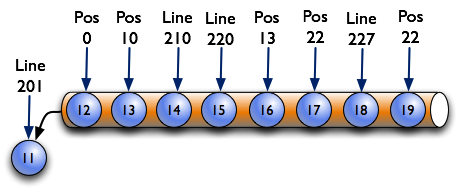
\includegraphics[width=1.0\textwidth]{figures/example-buffer.png}
  \caption{Example Buffer}
  \label{fig:example-buffer}
\end{figure}

\FloatBarrier

If an \gls{agent} receives a \gls{sample request} from a client software application, the \gls{agent} \MUST publish an \gls{mtconnectstreams response document} that contains a range of data values.  The range of values are defined by the \gls{from query} and \gls{count model} parameters that must be included as part of the \gls{sample request}.  If the value of \gls{from query} is 14 and the value of \gls{count model} is 5, the \gls{agent} \MUST publish an \gls{mtconnectstreams response document} that includes five (5) pieces of data represented by \glspl{sequence number} 14, 15, 16, 17, and 18 - three (3) occurrences of \cfont{Line} and two (2) occurrences of \cfont{Pos}.  In this case, \gls{nextsequence} will also be returned with a value of 19.

Likewise, if the same \gls{agent} receives a \gls{current request} from a client software application, the \gls{agent} \MUST publish an \gls{mtconnectstreams response document} that contains the most current information available for each of the types of data that is being published to the \gls{agent}.  In this case, the specific data that \MUST be represented in the \gls{mtconnectstreams response document} is \cfont{Pos} with a value of 22 and a \gls{sequence number} of 19 and \cfont{Line} with a value of 227 and a \gls{sequence number} of 18.

There is also a derivation of the \gls{current request} that will cause an \gls{agent} to publish an \gls{mtconnectstreams response document} that contains a set of data relative to a specific sequence number.  The \gls{current request} \MAY include an additional parameter called \gls{at query}.  When the \gls{at query} parameter, along with an \gls{instanceid}, is included as part of a \gls{current request}, an \gls{agent} \MUST publish an \gls{mtconnectstreams response document} that contains the most current information available for each of the types of \glspl{data entity} that are being published to the \gls{agent} that occur immediately at or before the \gls{sequence number} specified with the \gls{at query} parameter.

For example, if the \gls{request} is \cfont{current?at=15}, an \gls{agent} \MUST publish a \gls{mtconnectstreams response document} that contains the most current information available for each of the \glspl{data entity} that are stored in the \gls{buffer} of the \gls{agent} with a \gls{sequence number} of 15 or lower.  In this case, the specific data that \MUST be represented in the \gls{mtconnectstreams response document} is \cfont{Pos} with a value of 10 and a \gls{sequence number} of 13 and \cfont{Line} with a value of 220 and a \gls{sequence number} of 15.

If a \gls{current httprequest} \gls{request} is received for a \gls{sequence number} of 11 or lower, an \gls{agent} \MUST return an \gls{outofrange value} \gls{mtconnecterrors response document}.  The same \gls{http error message} \MUST be given if a \gls{sequence number} is requested that is greater than the end of the \gls{buffer}.  See \sect{Error Information Model} for more information on \gls{mtconnecterrors response document}.

\subsubsection{Accessing MTConnect Assets Information from an Agent}

When an \gls{agent} receives an \gls{asset request}, the \gls{agent} \MUST publish an \gls{mtconnectassets} document that contains information regarding the \glspl{asset document} that are stored in the \gls{agent}.

See \citetitle{MTCPart40} for details on \glspl{mtconnect asset}, \glspl{asset request}, and the \gls{mtconnectassets response document}.

\section{XML Representation of Response Documents}
\label{sec:XML Representation of Response Documents}

As defined in \sect{XML Documents}, \gls{xml} is currently the only language supported by the MTConnect Standard for encoding \glspl{response document}.

\glspl{response document} must be valid and conform to the \gls{schema} defined in the \gls{semantic data model} defined for that document.  The \gls{schema} for each \gls{response document} \MUST be updated to correlate to a specific version of the MTConnect Standard.  Versions, within a \gls{major} version, of the MTConnect Standard will be defined in such a way to best maintain backwards compatibility of the \glspl{semantic data model} through all \gls{minor} revisions of the Standard.  However, new \gls{minor} versions may introduce extensions or enhancements to existing \glspl{semantic data model}.

To be valid, a \gls{response document} must be well-formed; meaning that, amongst other things, each element has the required \gls{xml} \textit{start-tag} and \textit{end-tag} and that the document does not contain any illegal characters.  The validation of the document may also include a determination that required elements and attributes are present, they only occur in the appropriate location in the document, and they appear only the correct number of times.  If the document is not well-formed, it may be rejected by a client software application.  The \gls{semantic data model} defined for each \gls{response document} also specifies the elements and \glspl{child element} that may appear in a document.  \gls{xml} elements may contain \glspl{child element}, \gls{cdata}, or both.  The \gls{semantic data model} also defines the number of times each element and \gls{child element} may appear in the document.

Each \gls{response document} encoded using \gls{xml} consists of the following primary sections:

\begin{itemize}
\item \gls{xml} Declaration

\item Root Element

\item Schema and Namespace Declaration

\item Document Header

\item Document Body
\end{itemize}

The following will provide details defining how each of the \glspl{response document} are encoded using \gls{xml}.

\begin{note}
Note: See \sect{Terminology and Conventions} for the definition of \gls{xml} related terms used in the MTConnect Standard.

\end{note}

\subsection{Fundamentals of Using XML to Encode Response Documents}

The MTConnect Standard follows industry conventions for formatting the elements and attributes included in an \gls{xml} document.  The general guidelines are as follows: 

\begin{itemize}
\item All element names \MUST be specified in Pascal case (first letter of each word is capitalized). For example: \cfont{<PowerSupply/>}.

\item The name for an attribute \MUST be Camel case; similar to Pascal case, but the first letter will be lower case.  For example: \cfont{<MyElement nativeName="bob"/>} where \cfont{MyElement} is the \gls{element name} and \gls{nativename} is an attribute.

\item All \gls{cdata} values that are defined with a limited or controlled vocabulary \MUST be in upper case with an \_ (underscore) separating words.  For example: \gls{on value}, \gls{off value}, \gls{actual subtype}, and \gls{counterclockwise value}.

\item The values provided for a date and/or a time \MUST follow the W3C ISO 8601 format with an arbitrary number of decimals representing fractions of a second.  Refer to the following specification for details on the format for dates and times:  http://www.w3.org/TR/NOTE-datetime.

The format for the value describing a date and a time will be\\ YYYY-MM-DDThh:mm:ss.ffff. An example would be: 2017-01-13T13:01.213415Z.  

\begin{note}
Note:  Z refers to UTC/GMT time, not local time.

\end{note}

The accuracy and number of decimals representing fractions of a second for a \gls{timestamp} \MUST be determined by the capabilities of the piece of equipment publishing information to an \gls{agent}.  All time values \MUST be provided in UTC (GMT).

\item \gls{xml} element names \MUST be spelled out and abbreviations are not permitted.   See the exclusion below regarding the use of the suffix \cfont{Ref}.

\item \gls{xml} attribute names \SHOULD be spelled out and abbreviations \SHOULD be avoided.  The exception to this rule is the use of \gls{id} when associated with an identifier.  See the exclusion below regarding the use of the suffix \cfont{Ref}.

\item The abbreviation \cfont{Ref} for \gls{reference} is permitted as a suffix to element names of either a \gls{structural element} or a \gls{data entity} to provide an efficient method to associate information defined in another location in a \gls{data model} without duplicating that original data or structure.  See \textit{Section 4.8} in \citetitle{MTCPart2} for more information on \gls{reference}.
\end{itemize}

\subsection{XML Declaration}

The first section of a \gls{response document} encoded with \gls{xml} \SHOULD be the \gls{xml declaration}.  The declaration is a single element.

An example of an \gls{xml declaration} would be:  

\begin{lstlisting}[firstnumber=1,escapechar=|,%
caption={Example of xml declaration}, label={lst:xml-declaration}]
<?xml version="1.0" encoding="UTF-8"?>
\end{lstlisting}

This element provides information regarding how the \gls{xml} document is encoded and the character type used for that encoding.  See the W3C website for more details on the \gls{xml} declaration. 

\subsection{Root Element}

Every \gls{response document} \MUST contain only one root element.  The MTConnect Standard defines \gls{mtconnectdevices}, \gls{mtconnectstreams}, \gls{mtconnectassets}, and \gls{mtconnecterror} as \glspl{root element}. 

The \gls{root element} specifies a specific \gls{response document} and appears at the top of the document immediately following the \gls{xml declaration}.

\subsubsection{MTConnectDevices Root Element}

\gls{mtconnectdevices} is the \gls{root element} for the \gls{mtconnectdevices response document}.  

\begin{figure}[ht]
  \centering
  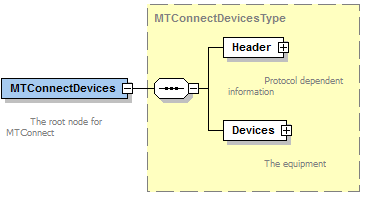
\includegraphics[width=0.7\textwidth]{figures/mtconnectdevices-structure.png}
  \caption{MTConnectDevices Structure}
  \label{fig:mtconnectdevices-structure}
\end{figure}

\FloatBarrier

\gls{mtconnectdevices} \MUST contain two \glspl{child element} - \gls{header} and \gls{devices}.  Details for \gls{header} are defined in \sect{Document Header}.  

\gls{devices} is an \gls{xml} container that represents the \gls{document body} for an \gls{mtconnectdevices response document} - see \sect{Document Body}.  Details for the \gls{semantic data model} describing the contents for \gls{devices} are defined in \citetitle{MTCPart2}.

\gls{mtconnectdevices} also has a number of attributes.  These attributes are defined in \sect{Schema and Namespace Declaration}.

\paragraph{MTConnectDevices Elements}\mbox{}

An \gls{mtconnectdevices} element \MUST contain a \gls{header} and a \gls{devices} element.

\tabulinesep = 5pt
\begin{longtabu} to \textwidth {
    |l|X[3l]|X[0.75l]|}
\caption{Elements for MTConnectDevices} \label{table:elements-for-mtconnectdevices} \\

\hline
Element & Description & Occurrence \\
\hline
\endfirsthead

\hline
\multicolumn{3}{|c|}{Continuation of Table \ref{table:elements-for-mtconnectdevices}}\\
\hline
Element & Description & Occurrence \\
\hline
\endhead

\gls{header}
&
An \gls{xml} container in an \gls{mtconnect response document} that provides information from an \gls{agent} defining version information, storage capacity, and parameters associated with the data management within the \gls{agent}.
&
1 \\
\hline

\gls{devices}
&
The \gls{xml} container in an \gls{mtconnect response document} that provides the \gls{equipment metadata} for each of the pieces of equipment associated with an \gls{agent}.
&
1 \\
\hline


\end{longtabu}

\subsubsection{MTConnectStreams Root Element}

\gls{mtconnectstreams} is the \gls{root element} for the \gls{mtconnectstreams response document}.  

\begin{figure}[ht]
  \centering
  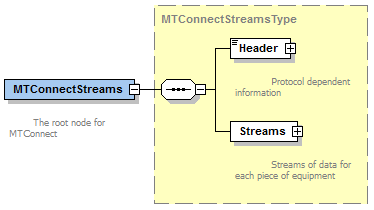
\includegraphics[width=0.7\textwidth]{figures/mtconnectstreams-structure.png}
  \caption{MTConnectStreams Structure}
  \label{fig:mtconnectstreams-structure}
\end{figure}

\FloatBarrier

\gls{mtconnectstreams} \MUST contain two \glspl{child element} - \gls{header} and \gls{streams}.  

Details for \gls{header} are defined in \sect{Document Header}.  

\gls{streams} is an \gls{xml} container that represents the \gls{document body} for a \gls{mtconnectstreams response document} - see \sect{Document Body}.  Details for the \gls{semantic data model} describing the contents for \gls{streams} are defined in \citetitle{MTCPart3}.

\gls{mtconnectstreams} also has a number of attributes.  These attributes are defined in \sect{Schema and Namespace Declaration}.

\newpage

\paragraph{MTConnectStreams Elements}\mbox{}

An \gls{mtconnectstreams} element \MUST contain a \gls{header} and a \gls{streams} element.

\tabulinesep = 5pt
\begin{longtabu} to \textwidth {
    |l|X[3l]|X[0.75l]|}
\caption{Elements for MTConnectStreams} \label{table:elements-for-mtconnectstreams} \\

\hline
Element & Description & Occurrence \\
\hline
\endfirsthead

\hline
\multicolumn{3}{|c|}{Continuation of Table \ref{table:elements-for-mtconnectstreams}}\\
\hline
Element & Description & Occurrence \\
\hline
\endhead

\gls{header}
&
An \gls{xml} container in an \gls{mtconnect response document} that provides information from an \gls{agent} defining version information, storage capacity, and parameters associated with the data management within the \gls{agent}.
&
1 \\
\hline

\gls{streams}
&
The \gls{xml} container for the information published by an \gls{agent} in a \gls{mtconnectstreams response document}.
&
1 \\
\hline


\end{longtabu}

\subsubsection{MTConnectAssets Root Element}

\gls{mtconnectassets} is the \gls{root element} for the \gls{mtconnectassets response document}.  

\begin{figure}[ht]
  \centering
  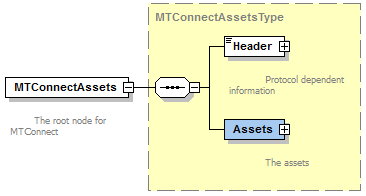
\includegraphics[width=0.7\textwidth]{figures/mtconnectassets-structure.png}
  \caption{MTConnectAssets Structure}
  \label{fig:mtconnectassets-structure}
\end{figure}

\FloatBarrier

\newpage 

\gls{mtconnectassets} \MUST contain two \glspl{child element} - \gls{header} and \gls{assets mtconnectassets}.

Details for \gls{header} are defined in \sect{Document Header}.  

\gls{assets mtconnectassets} is an \gls{xml} container that represents the \gls{document body} for an \gls{mtconnectassets response document} - see \sect{Document Body}.  Details for the \gls{semantic data model} describing the contents for \gls{assets mtconnectassets} are defined in \citetitle{MTCPart40}.

\gls{mtconnectassets} also has a number of attributes.  These attributes are defined in \sect{Schema and Namespace Declaration}.

\paragraph{MTConnectAssets Elements}\mbox{}

An \gls{mtconnectassets} element \MUST contain a \gls{header} and an \gls{assets mtconnectassets} element.

\tabulinesep = 5pt
\begin{longtabu} to \textwidth {
    |l|X[3l]|X[0.75l]|}
\caption{Elements for MTConnectAssets} \label{table:elements-for-mtconnectassets} \\

\hline
Element & Description & Occurrence \\
\hline
\endfirsthead

\hline
\multicolumn{3}{|c|}{Continuation of Table \ref{table:elements-for-mtconnectassets}}\\
\hline
Element & Description & Occurrence \\
\hline
\endhead

\gls{header}
&
An \gls{xml} container in an \gls{mtconnect response document} that provides information from an \gls{agent} defining version information, storage capacity, and parameters associated with the data management within the \gls{agent}.
&
1 \\
\hline

\gls{assets mtconnectassets}
&
The \gls{xml} container in an \gls{mtconnectassets response document} that provides information for \glspl{mtconnect asset} associated with an \gls{agent}.
&
1 \\
\hline


\end{longtabu}

\subsubsection{MTConnectError Root Element}

\gls{mtconnecterror} is the \gls{root element} for the \gls{mtconnecterrors response document}.

\begin{figure}[ht]
  \centering
  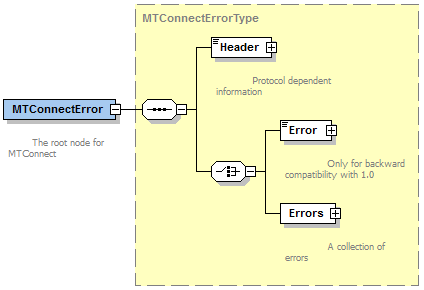
\includegraphics[width=0.7\textwidth]{figures/mtconnecterror-structure.png}
  \caption{MTConnectError Structure}
  \label{fig:mtconnecterror-structure}
\end{figure}

\FloatBarrier

\gls{mtconnecterror} \MUST contain two \glspl{child element} - \gls{header} and \gls{errors}. 

\begin{note}
Note:	When compatibility with \textit{Version 1.0.1} and earlier of the MTConnect Standard is required for an implementation, the \gls{mtconnecterrors response document} contains only a single \gls{error} \gls{data entity} and the \gls{errors} \gls{child element} \MUSTNOT appear in the document. 

\end{note}

Details for \gls{header} are defined in \sect{Document Header}.  

\gls{errors} is an \gls{xml} container that represents the \gls{document body} for an \gls{mtconnecterrors response document} - See \sect{Document Body}.  Details for the \gls{semantic data model} describing the contents for \gls{errors} are defined in \sect{Error Information Model}.

\gls{mtconnecterror} also has a number of attributes.  These attributes are defined in \sect{Schema and Namespace Declaration}.

\paragraph{MTConnectError Elements}\mbox{}

An \gls{mtconnecterror} element \MUST contain a \gls{header} and an \gls{errors} element.

\tabulinesep = 5pt
\begin{longtabu} to \textwidth {
    |l|X[3l]|X[0.75l]|}
\caption{Elements for MTConnectError} \label{table:elements-for-mtconnecterror} \\

\hline
Element & Description & Occurrence \\
\hline
\endfirsthead

\hline
\multicolumn{3}{|c|}{Continuation of Table \ref{table:elements-for-mtconnecterror}}\\
\hline
Element & Description & Occurrence \\
\hline
\endhead

\gls{header}
&
An \gls{xml} container in an \gls{mtconnect response document} that provides information from an \gls{agent} defining version information, storage capacity, and parameters associated with the data management within the \gls{agent}.
&
1 \\
\hline

\gls{errors}
&
The \gls{xml} container in an \gls{mtconnecterrors response document} that provides information associated with errors encountered by an \gls{agent}.
&
1 \\
\hline


\end{longtabu}

\subsection{Schema and Namespace Declaration}
\label{sec:Schema and Namespace Declaration}

\gls{xml} provides standard methods for declaring the \gls{schema} and \gls{namespace} associated with a document encoded by \gls{xml}.  The declaration of the \gls{schema} and \gls{namespace} for MTConnect \glspl{response document} \MUST be structured as attributes in the \gls{root element} of the document.  \gls{xml} defines these attributes as pseudo-attributes since they provide additional information for the entire document and not just specifically for the \gls{root element} itself.  

\begin{note}
Note:	If a \gls{response document} contains sections that utilize different \glspl{schema} and/or \glspl{namespace}, additional pseudo-attributes should appear in the document as declared using standard conventions as defined be W3C.

\end{note}

For further information on declarations refer to \apx{Schema and Namespace Declaration Information}.

\subsection{Document Header}
\label{sec:Document Header}

The \gls{document header} is an \gls{xml} container in an \gls{mtconnect response document} that provides information from an \gls{agent} defining version information, storage capacity, and parameters associated with the data management within the \gls{agent}.  This \gls{xml} element is called \gls{header}.

\gls{header} \MUST be the first \gls{xml} element following the \gls{root element} of any \gls{response document}.  The \gls{header} \gls{xml} element \MUSTNOT contain any \glspl{child element}.  

The content of the \gls{header} element will be different for each type of \gls{response document}.

\subsubsection{Header for MTConnectDevices}

The \gls{header} element for an \gls{mtconnectdevices response document} defines information regarding the creation of the document and the data storage capability of the \gls{agent} that generated the document.  

\paragraph{XML Schema Structure for Header for MTConnectDevices}\mbox{}

The \gls{xml schema} in \fig{header-schema-diagram-for-mtconnectdevices} represents the structure of the \gls{header} \gls{xml} element that \MUST be provided for an \gls{mtconnectdevices response document}.  

\begin{figure}[ht]
  \centering
  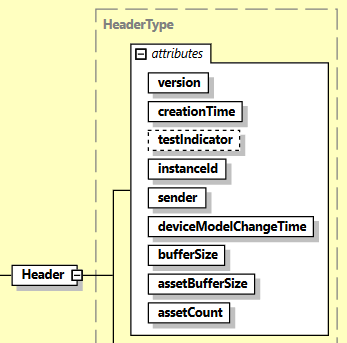
\includegraphics[width=0.6\textwidth]{figures/header-schema-diagram-for-mtconnectdevices.png}
  \caption{Header Schema Diagram for MTConnectDevices}
  \label{fig:header-schema-diagram-for-mtconnectdevices}
\end{figure}

\FloatBarrier

\paragraph{Attributes for Header for MTConnectDevices}\mbox{}

\tbl{attributes-for-header-mtconnectdevices} defines the attributes that may be used to provide additional information in the \gls{header} element for an \gls{mtconnectdevices response document}. 

\tabulinesep = 5pt
\begin{longtabu} to \textwidth {
    |l|X[3l]|X[0.75l]|}
\caption{MTConnectDevices Header} \label{table:attributes-for-header-mtconnectdevices} \\

\hline
Attribute & Description & Occurrence \\
\hline
\endfirsthead

\hline
\multicolumn{3}{|c|}{Continuation of Table \ref{table:attributes-for-header-mtconnectdevices}}\\
\hline
Attribute & Description & Occurrence \\
\hline
\endhead

\gls{version}
&
The \gls{major}, \gls{minor}, and \gls{revision} number of the MTConnect Standard that defines the \gls{semantic data model} that represents the content of the \gls{response document}.   It also includes the revision number of the \gls{schema} associated with that specific \gls{semantic data model}.
\newline The value reported for \gls{version} \MUST be a series of four numeric values, separated by a decimal point, representing a \gls{major}, \gls{minor}, and \gls{revision} number of the MTConnect Standard and the revision number of a specific \gls{schema}.  
\newline As an example, the value reported for \gls{version} for a \gls{response document} that was structured based on \gls{schema} revision 10 associated with Version 1.4.0 of the MTConnect Standard would be:  1.4.0.10
\newline \gls{version} is a required attribute.
&
1 \\
\hline

\gls{creationtime}
&
\gls{creationtime} represents the time that an \gls{agent} published the \gls{response document}. 
\newline \gls{creationtime} \MUST be reported in UTC (Coordinated Universal Time) format; e.g., "2010-04-01T21:22:43Z".
\newline Note:  Z refers to UTC/GMT time, not local time.
\newline \gls{creationtime} is a required attribute.
&
1 \\
\hline

\gls{testindicator}
&
A flag indicating that the \gls{agent} that published the \gls{response document} is operating in a test mode.  The contents of the \gls{response document} may not be valid and SHOULD be used for testing and simulation purposes only. 
\newline The values reported for \gls{testindicator} are:
\newline -	  \DIFadd{\gls{true value}}:  The \gls{agent} is functioning in a test mode.
\newline -	  \DIFadd{\gls{false value}}:  The \gls{agent} is not functioning in a test mode.
\newline If \gls{testindicator} is not specified, the value for \gls{testindicator} \MUST be interpreted to be \gls{false value}.
\newline \gls{testindicator} is an optional attribute.
&
0..1 \\
\hline

\gls{instanceid}
&
A number indicating a specific instantiation of the \gls{buffer} associated with the \gls{agent} that published the \gls{response document}.  
\newline The value reported for \gls{instanceid} \MUST be a unique unsigned 64-bit integer.   
\newline The value for \gls{instanceid} \MUST be changed to a different unique number each time the \gls{buffer} is cleared and a new set of data begins to be collected.
\newline \gls{instanceid} is a required attribute.
&
1 \\
\hline

\gls{sender}
&
An identification defining where the \gls{agent} that published the \gls{response document} is installed or hosted.
\newline The value reported for \gls{sender} \MUST be either an IP Address or Hostname describing where the \gls{agent} is installed or the URL of the \gls{agent}; e.g., \cfont{http://<address>[:port]/}. 
\newline Note:  The port number need not be specified if it is the default HTTP port 80.
\newline \gls{sender} is a required attribute.
&
1 \\
\hline

\gls{buffersize}
&
A value representing the maximum number of \glspl{data entity} that \MAY be retained in the \gls{agent} that published the \gls{response document} at any point in time.
\newline The value reported for \gls{buffersize} \MUST be a number representing an unsigned 32-bit integer.
\newline \gls{buffersize} is a required attribute. 
\newline Note 1:  \gls{buffersize} represents the maximum number of sequence numbers that \MAY be stored in the \gls{agent}. 
\newline Note 2: The implementer is responsible for allocating the appropriate amount of storage capacity required to accommodate the \gls{buffersize}.
&
1 \\
\hline


\gls{assetbuffersize}
&
A value representing the maximum number of \glspl{asset document} that can be stored in the \gls{agent} that published the \gls{response document}.  
\newline The value reported for \gls{assetbuffersize} \MUST be a number representing an unsigned 32-bit integer.
\newline \gls{assetbuffersize} is a required attribute.
\newline Note: The implementer is responsible for allocating the appropriate amount of storage capacity required to accommodate the \gls{assetbuffersize}.
&
1 \\
\hline

\gls{assetcount}
&
A number representing the current number of \glspl{asset document} that are currently stored in the \gls{agent} as of the \gls{creationtime} that the \gls{agent} published the \gls{response document}.  
\newline The value reported for \gls{assetcount} \MUST be a number representing an unsigned 32-bit integer and \MUSTNOT be larger than the value reported for \gls{assetbuffersize}.
\newline \gls{assetcount} is a required attribute.
&
1 \\
\hline


\DIFaddbegin \DIFadd{\gls{devicemodelchangetime}
}&
\DIFadd{\glsentrydesc{devicemodelchangetime}
}&
\DIFadd{1 }\\
\hline


\DIFaddend \end{longtabu}

\lst{header-xml-element-for-mtconnectdevices} is an example of a \gls{header} \gls{xml} element for an \gls{mtconnectdevices response document}:

\begin{lstlisting}[firstnumber=1,escapechar=|,%
caption={Example of Header XML Element for MTConnectDevices}, label={lst:header-xml-element-for-mtconnectdevices}]
<Header creationTime="2017-02-16T16:44:27Z"
  sender="MyAgent" instanceId="1268463594"
  bufferSize="131072" version="1.4.0.10"
  assetCount="54" assetBufferSize="1024"/>
\end{lstlisting}

\subsubsection{Header for MTConnectStreams}

The \gls{header} element for an \gls{mtconnectstreams response document} defines information regarding the creation of the document and additional information necessary for an application to interact and retrieve data from the \gls{agent}.

\paragraph{XML Schema Structure for Header for MTConnectStreams}\mbox{}

The \gls{xml schema} in \fig{header-schema-diagram-for-mtconnectstreams} represents the structure of the \gls{header} \gls{xml} element that \MUST be provided for an \gls{mtconnectstreams response document}.  

\begin{figure}[ht]
  \centering
  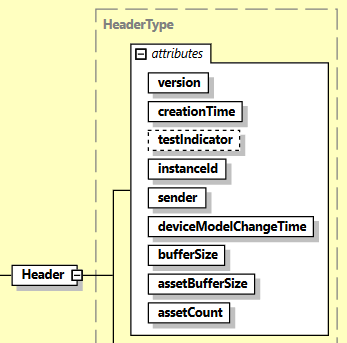
\includegraphics[width=0.6\textwidth]{figures/header-schema-diagram-for-mtconnectstreams.png}
  \caption{Header Schema Diagram for MTConnectStreams}
  \label{fig:header-schema-diagram-for-mtconnectstreams}
\end{figure}

\FloatBarrier

\paragraph{Attributes for MTConnectStreams Header}\mbox{}

\tbl{attributes-for-header-mtconnectstreams} defines the attributes that may be used to provide additional information in the \gls{header} element for an \gls{mtconnectstreams response document}.

\tabulinesep = 5pt
\begin{longtabu} to \textwidth {
    |l|X[3l]|X[0.75l]|}
\caption{MTConnectStreams Header} \label{table:attributes-for-header-mtconnectstreams} \\

\hline
Attribute & Description & Occurrence \\
\hline
\endfirsthead

\hline
\multicolumn{3}{|c|}{Continuation of Table \ref{table:attributes-for-header-mtconnectstreams}}\\
\hline
Attribute & Description & Occurrence \\
\hline
\endhead

\gls{version}
&
The \gls{major}, \gls{minor}, and \gls{revision} number of the MTConnect Standard that defines the \gls{semantic data model} that represents the content of the \gls{response document}.   It also includes the revision number of the \gls{schema} associated with that specific \gls{semantic data model}.
\newline The value reported for \gls{version} \MUST be a series of four numeric values, separated by a decimal point, representing a \gls{major}, \gls{minor}, and \gls{revision} number of the MTConnect Standard and the revision number of a specific \gls{schema}.  
\newline As an example, the value reported for \gls{version} for a \gls{response document} that was structured based on \gls{schema} revision 10 associated with Version 1.4.0 of the MTConnect Standard would be:  1.4.0.10
\newline \gls{version} is a required attribute.
&
1 \\
\hline

\gls{creationtime}
&
\gls{creationtime} represents the time that an \gls{agent} published the \gls{response document}. 
\newline \gls{creationtime} \MUST be reported in UTC (Coordinated Universal Time) format; e.g., "2010-04-01T21:22:43Z".
\newline Note:  Z refers to UTC/GMT time, not local time.
\newline \gls{creationtime} is a required attribute.
&
1 \\
\hline

\gls{nextsequence}
&
A number representing the \gls{sequence number} of the piece of \gls{streaming data} that is the next piece of data to be retrieved from the \gls{buffer} of the \gls{agent} that was not included in the Response Document published by the \gls{agent}.
\newline If the \gls{streaming data} included in the Response Document includes the last piece of data stored in the \gls{buffer} of the \gls{agent} at the time that the document was published, then the value reported for \gls{nextsequence} \MUST be equal to \gls{lastsequence} + 1.
\newline The value reported for \gls{nextsequence} \MUST be a number representing an unsigned 64-bit integer.
\newline \gls{nextsequence} is a required attribute.
&
1 \\
\hline

\gls{lastsequence}
&
A number representing the \gls{sequence number} assigned to the last piece of \gls{streaming data} that was added to the \gls{buffer} of the \gls{agent} immediately prior to the time that the \gls{agent} published the Response Document.   
\newline The value reported for \gls{lastsequence} \MUST be a number representing an unsigned 64-bit integer.
\newline \gls{lastsequence} is a required attribute.
&
1 \\
\hline

\gls{firstsequence}
&
A number representing the \gls{sequence number} assigned to the oldest piece of \gls{streaming data} stored in the \gls{buffer} of the \gls{agent} immediately prior to the time that the \gls{agent} published the Response Document.   
\newline The value reported for \gls{firstsequence} \MUST be a number representing an unsigned 64-bit integer.
\newline \gls{firstsequence} is a required attribute.
&
1 \\
\hline

\gls{testindicator}
&
A flag indicating that the \gls{agent} that published the \gls{response document} is operating in a test mode.  The contents of the \gls{response document} may not be valid and \SHOULD be used for testing and simulation purposes only. 
\newline The values reported for \gls{testindicator} are:
\newline -	  \DIFadd{\gls{true value}}:  The \gls{agent} is functioning in a test mode.
\newline -	  \DIFadd{\gls{false value}}:  The \gls{agent} is not functioning in a test mode.
\newline If \gls{testindicator} is not specified, the value for \gls{testindicator} \MUST be interpreted to be \gls{false value}.
\newline \gls{testindicator} is an optional attribute.
&
0..1 \\
\hline

\gls{instanceid}
&
A number indicating a specific instantiation of the \gls{buffer} associated with the \gls{agent} that published the \gls{response document}.  
\newline The value reported for \gls{instanceid} \MUST be a unique unsigned 64-bit integer.   
\newline The value for \gls{instanceid} \MUST be changed to a different unique number each time the \gls{buffer} is cleared and a new set of data begins to be collected.
\newline \gls{instanceid} is a required attribute.
&
1 \\
\hline

\gls{sender}
&
An identification defining where the \gls{agent} that published the \gls{response document} is installed or hosted.
\newline The value reported for \gls{sender} \MUST be either an IP Address or Hostname describing where the \gls{agent} is installed or the URL of the \gls{agent}; e.g., \cfont{http://<address>[:port]/}. 
\newline Note:  The port number need not be specified if it is the default HTTP port 80.
\newline \gls{sender} is a required attribute.
&
1 \\
\hline

\gls{buffersize}
&
A value representing the maximum number of \glspl{data entity} that \MAY be retained in the \gls{agent} that published the \gls{response document} at any point in time.
\newline The value reported for \gls{buffersize} \MUST be a number representing an unsigned 32-bit integer.
\newline \gls{buffersize} is a required attribute. 
\newline Note 1:  \gls{buffersize} represents the maximum number of  \glspl{sequence number} that \MAY be stored in the \gls{agent}. 
\newline Note 2: The implementer is responsible for allocating the appropriate amount of storage capacity required to accommodate the \gls{buffersize}.
&
1 \\
\hline

\DIFaddbegin \DIFadd{\gls{devicemodelchangetime}
}&
\DIFadd{\glsentrydesc{devicemodelchangetime}
}&
\DIFadd{1 }\\
\hline


\DIFaddend \end{longtabu}

\lst{header-xml-element-for-mtconnectstreams} is an example of a \gls{header} \gls{xml} element for an \gls{mtconnectstreams response document}:

\begin{lstlisting}[firstnumber=1,escapechar=|,%
caption={Example of Header XML Element for MTConnectStreams}, label={lst:header-xml-element-for-mtconnectstreams}]
<Header lastSequence="5430495" firstSequence="5299424"
  nextSequence="5430496" bufferSize="131072"
  version="1.4.0.12" instanceId="1579788747"
  sender="myagent" creationTime="2020-03-24T13:23:32Z"/>
\end{lstlisting}

\subsubsection{Header for MTConnectAssets}

The \gls{header} element for an \gls{mtconnectassets response document} defines information regarding the creation of the document and the storage of \glspl{asset document} in the \gls{agent} that generated the document.  

\paragraph{XML Schema Structure for Header for MTConnectAssets}\mbox{}

The \gls{xml schema} in \fig{header-schema-diagram-for-mtconnectassets} represents the structure of the \gls{header} \gls{xml} element that \MUST be provided for an \gls{mtconnectassets response document}.  

\begin{figure}[ht]
  \centering
  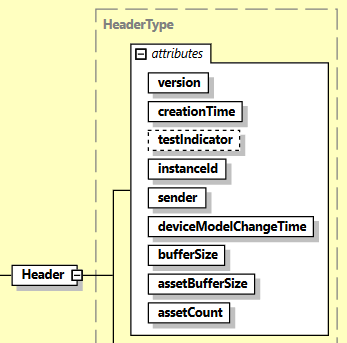
\includegraphics[width=0.6\textwidth]{figures/header-schema-diagram-for-mtconnectassets.png}
  \caption{Header Schema Diagram for MTConnectAssets}
  \label{fig:header-schema-diagram-for-mtconnectassets}
\end{figure}

\FloatBarrier

\paragraph{Attributes for Header for MTConnectAssets}\mbox{}

\tbl{attributes-for-header-mtconnectassets} defines the attributes that may be used to provide additional information in the \gls{header} element for an \gls{mtconnectassets response document}.

\tabulinesep = 5pt
\begin{longtabu} to \textwidth {
    |l|X[3l]|X[0.75l]|}
\caption{MTConnectAssets Header} \label{table:attributes-for-header-mtconnectassets} \\

\hline
Attribute & Description & Occurrence \\
\hline
\endfirsthead

\hline
\multicolumn{3}{|c|}{Continuation of Table \ref{table:attributes-for-header-mtconnectassets}}\\
\hline
Attribute & Description & Occurrence \\
\hline
\endhead

\gls{version}
&
The \gls{major}, \gls{minor}, and \gls{revision} number of the MTConnect Standard that defines the \gls{semantic data model} that represents the content of the \gls{response document}.   It also includes the revision number of the \gls{schema} associated with that specific \gls{semantic data model}.
\newline The value reported for \gls{version} \MUST be a series of four numeric values, separated by a decimal point, representing a \gls{major}, \gls{minor}, and \gls{revision} number of the MTConnect Standard and the revision number of a specific \gls{schema}.  
\newline As an example, the value reported for \gls{version} for a \gls{response document} that was structured based on \gls{schema} revision 10 associated with Version 1.4.0 of the MTConnect Standard would be:  1.4.0.10
\newline \gls{version} is a required attribute.
&
1 \\
\hline

\gls{creationtime}
&
\gls{creationtime} represents the time that an \gls{agent} published the \gls{response document}. 
\newline \gls{creationtime} \MUST be reported in UTC (Coordinated Universal Time) format; e.g., "2010-04-01T21:22:43Z".
\newline Note:  Z refers to UTC/GMT time, not local time.
\newline \gls{creationtime} is a required attribute.
&
1 \\
\hline

\gls{testindicator}
&
A flag indicating that the \gls{agent} that published the \gls{response document} is operating in a test mode.  The contents of the \gls{response document} may not be valid and SHOULD be used for testing and simulation purposes only. 
\newline The values reported for \gls{testindicator} are:
\newline -	  \DIFadd{\gls{true value}}:  The \gls{agent} is functioning in a test mode.
\newline -	  \DIFadd{\gls{false value}}:  The \gls{agent} is not functioning in a test mode.
\newline If \gls{testindicator} is not specified, the value for \gls{testindicator} \MUST be interpreted to be \gls{false value}.
\newline \gls{testindicator} is an optional attribute.
&
0..1 \\
\hline

\gls{instanceid}
&
A number indicating a specific instantiation of the \gls{buffer} associated with the \gls{agent} that published the \gls{response document}.  
\newline The value reported for \gls{instanceid} \MUST be a unique unsigned 64-bit integer.   
\newline The value for \gls{instanceid} \MUST be changed to a different unique number each time the \gls{buffer} is cleared and a new set of data begins to be collected.
\newline \gls{instanceid} is a required attribute.
&
1 \\
\hline

\gls{sender}
&
An identification defining where the \gls{agent} that published the \gls{response document} is installed or hosted.
\newline The value reported for \gls{sender} \MUST be either an IP Address or Hostname describing where the \gls{agent} is installed or the URL of the \gls{agent}; e.g., \cfont{http://<address>[:port]/}. 
\newline Note:  The port number need not be specified if it is the default HTTP port 80.
\newline \gls{sender} is a required attribute.
&
1 \\
\hline


\gls{assetbuffersize}
&
A value representing the maximum number of \glspl{asset document} that can be stored in the \gls{agent} that published the \gls{response document}.  
\newline The value reported for \gls{assetbuffersize} \MUST be a number representing an unsigned 32-bit integer.
\newline \gls{assetbuffersize} is a required attribute.
\newline Note: The implementer is responsible for allocating the appropriate amount of storage capacity required to accommodate the \gls{assetbuffersize}.
&
1 \\
\hline

\gls{assetcount}
&
A number representing the current number of \glspl{asset document} that are currently stored in the \gls{agent} as of the \gls{creationtime} that the \gls{agent} published the \gls{response document}.  
\newline The value reported for \gls{assetcount} \MUST be a number representing an unsigned 32-bit integer and \MUSTNOT be larger than the value reported for \gls{assetbuffersize}.
\newline \gls{assetcount} is a required attribute.
&
1 \\
\hline

\DIFaddbegin \DIFadd{\gls{devicemodelchangetime}
}&
\DIFadd{\glsentrydesc{devicemodelchangetime}
}&
\DIFadd{1 }\\
\hline


\DIFaddend \end{longtabu}

\lst{header-xml-element-for-mtconnectassets} is an example of a \gls{header} \gls{xml} element for an \gls{mtconnectassets response document}:

\begin{lstlisting}[firstnumber=1,escapechar=|,%
caption={Example of Header XML Element for MTConnectAssets}, label={lst:header-xml-element-for-mtconnectassets}]
<Header creationTime="2017-02-16T16:44:27Z"
  sender="MyAgent" instanceId="1268463594"
  version="1.4.0.10" assetCount="54"
  assetBufferSize="1024"/>
\end{lstlisting}

\subsubsection{Header for MTConnectError}
\label{sec:Header for MTConnectError}

The \gls{header} element for an \gls{mtconnecterrors response document} defines information regarding the creation of the document and the data storage capability of the \gls{agent} that generated the document.  

\paragraph{XML Schema Structure for Header for MTConnectError}\mbox{}

The \gls{xml schema} in \fig{header-schema-diagram-for-mtconnecterror} represents the structure of the \gls{header} \gls{xml} element that \MUST be provided for an \gls{mtconnecterrors response document}.  

\begin{figure}[ht]
  \centering
  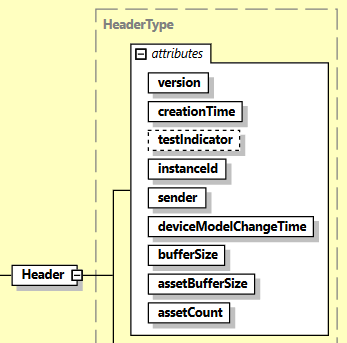
\includegraphics[width=0.6\textwidth]{figures/header-schema-diagram-for-mtconnecterror.png}
  \caption{Header Schema Diagram for MTConnectError}
  \label{fig:header-schema-diagram-for-mtconnecterror}
\end{figure}

\FloatBarrier

\paragraph{Attributes for Header for MTConnectError}\mbox{}

\tbl{attributes-for-header-mtconnecterror} defines the attributes that may be used to provide additional information in the \gls{header} element for an \gls{mtconnecterrors response document}. 

\tabulinesep = 5pt
\begin{longtabu} to \textwidth {
    |l|X[3l]|X[0.75l]|}
\caption{MTConnectError Header} \label{table:attributes-for-header-mtconnecterror} \\

\hline
Attribute & Description & Occurrence \\
\hline
\endfirsthead

\hline
\multicolumn{3}{|c|}{Continuation of Table \ref{table:attributes-for-header-mtconnecterror}}\\
\hline
Attribute & Description & Occurrence \\
\hline
\endhead

\gls{version}
&
The \gls{major}, \gls{minor}, and \gls{revision} number of the MTConnect Standard that defines the \gls{semantic data model} that represents the content of the \gls{response document}.   It also includes the revision number of the \gls{schema} associated with that specific \gls{semantic data model}.
\newline The value reported for \gls{version} \MUST be a series of four numeric values, separated by a decimal point, representing a \gls{major}, \gls{minor}, and \gls{revision} number of the MTConnect Standard and the revision number of a specific \gls{schema}.  
\newline As an example, the value reported for \gls{version} for a \gls{response document} that was structured based on \gls{schema} revision 10 associated with Version 1.4.0 of the MTConnect Standard would be:  1.4.0.10
\newline \gls{version} is a required attribute.
&
1 \\
\hline

\gls{creationtime}
&
\gls{creationtime} represents the time that an \gls{agent} published the \gls{response document}. 
\newline \gls{creationtime} \MUST be reported in UTC (Coordinated Universal Time) format; e.g., "2010-04-01T21:22:43Z".
\newline Note:  Z refers to UTC/GMT time, not local time.
\newline \gls{creationtime} is a required attribute.
&
1 \\
\hline

\gls{testindicator}
&
A flag indicating that the \gls{agent} that published the \gls{response document} is operating in a test mode.  The contents of the \gls{response document} may not be valid and SHOULD be used for testing and simulation purposes only. 
\newline The values reported for \gls{testindicator} are:
\newline -	  \DIFadd{\gls{true value}}:  The \gls{agent} is functioning in a test mode.
\newline -	  \DIFadd{\gls{false value}}:  The \gls{agent} is not functioning in a test mode.
\newline If \gls{testindicator} is not specified, the value for \gls{testindicator} \MUST be interpreted to be \gls{false value}.
\newline \gls{testindicator} is an optional attribute.
&
0..1 \\
\hline

\gls{instanceid}
&
A number indicating a specific instantiation of the \gls{buffer} associated with the \gls{agent} that published the \gls{response document}.  
\newline The value reported for \gls{instanceid} \MUST be a unique unsigned 64-bit integer.   
\newline The value for \gls{instanceid} \MUST be changed to a different unique number each time the \gls{buffer} is cleared and a new set of data begins to be collected.
\newline \gls{instanceid} is a required attribute.
&
1 \\
\hline

\gls{sender}
&
An identification defining where the \gls{agent} that published the \gls{response document} is installed or hosted.
\newline The value reported for \gls{sender} \MUST be either an IP Address or Hostname describing where the \gls{agent} is installed or the URL of the \gls{agent}; e.g., \cfont{http://<address>[:port]/}. 
\newline Note:  The port number need not be specified if it is the default HTTP port 80.
\newline \gls{sender} is a required attribute.
&
1 \\
\hline

\gls{buffersize}
&
A value representing the maximum number of \glspl{data entity} that \MAY be retained in the \gls{agent} that published the \gls{response document} at any point in time.
\newline The value reported for \gls{buffersize} \MUST be a number representing an unsigned 32-bit integer.
\newline \gls{buffersize} is a required attribute. 
\newline Note 1:  \gls{buffersize} represents the maximum number of sequence numbers that \MAY be stored in the \gls{agent}. 
\newline Note 2: The implementer is responsible for allocating the appropriate amount of storage capacity required to accommodate the \gls{buffersize}.
&
1 \\
\hline

\DIFaddbegin \DIFadd{\gls{devicemodelchangetime}
}&
\DIFadd{\glsentrydesc{devicemodelchangetime}
}&
\DIFadd{1 }\\
\hline


\DIFaddend \end{longtabu}

\lst{header-xml-element-for-mtconnecterror} is an example of a \gls{header} \gls{xml} element for an \gls{mtconnecterrors response document}:

\begin{lstlisting}[firstnumber=1,escapechar=|,%
caption={Example of Header XML Element for MTConnectError}, label={lst:header-xml-element-for-mtconnecterror}]
<Header creationTime="2017-02-16T16:44:27Z" 
  sender="MyAgent" instanceId="1268463594"
  bufferSize="131072" version="1.4.0.10"/>
\end{lstlisting}

\subsection{Document Body}
\label{sec:Document Body}

The \gls{document body} contains the information that is published by an \gls{agent} in response to a \gls{request} from a client software application.  Each \gls{response document} has a different \gls{xml} element that represents the \gls{document body}.

The structure of the content of the \gls{xml} element representing the \gls{document body} is defined by the \glspl{semantic data model} defined for each \gls{response document}.

\tbl{responsedocument-documentbody-semanticdatamodel} defines the relationship between each of the \glspl{response document}, the \gls{xml} element that represents the \gls{document body} for each document, and the \gls{semantic data model} that defines the structure for the content of each of the \glspl{response document}:

\tabulinesep = 5pt
\begin{longtabu} to \textwidth {
    |l|X[2l]|X[3l]|}
\caption{Relationship between Response Document and Semantic Data Model} \label{table:responsedocument-documentbody-semanticdatamodel} \\

\hline
Response Document & XML Element for Document Body & Semantic Data Model \\
\hline
\endfirsthead

\hline
\multicolumn{3}{|c|}{Continuation of Table \ref{table:responsedocument-documentbody-semanticdatamodel}}\\
\hline
Response Document & XML Element for Document Body & Semantic Data Model \\
\hline
\endhead

\gls{mtconnectdevices response document}
&
\gls{devices}
&
\citetitle{MTCPart2} \\
\hline

\gls{mtconnectstreams response document}
&
\gls{streams}
&
\citetitle{MTCPart3} \\
\hline

\gls{mtconnectassets response document}
&
\gls{assets mtconnectassets}
&
\citetitle{MTCPart40} \\
\hline

\gls{mtconnecterrors response document}
&
\gls{errors}
\newline Note:  \gls{errors} \MUSTNOT be used when backwards compatibility with MTConnect Standard Version 1.0.1 and earlier is required.
&
\citetitle{MTCPart1} \\
\hline

\end{longtabu}

\subsection{Extensibility}
\label{sec:Extensibility}

MTConnect is an extensible standard, which means that implementers \MAY extend the \glspl{data model} defined in the various sections of the MTConnect Standard to include information required for a specific implementation.  When these \glspl{data model} are encoded using \gls{xml}, the methods for extending these \glspl{data model} are defined by the rules established for extending any \gls{xml} schema (see the W3C website for more details on extending \gls{xml} data models).

The following are typical extensions that \MAY be considered in the MTConnect \glspl{data model}:

\begin{itemize}

\item Additional \gls{type} and \gls{subtype} values for \glspl{data entity}.

\item Additional \glspl{structural element} as containers.

\item Additional Composition elements.

\item New \gls{asset} types that are sub-typed from the abstract \gls{asset} type.

\item \glspl{child element} that may be added to specific \gls{xml} elements contained within the \glspl{mtconnect information model}.  These extended elements \MUST be identified in a separate \gls{namespace}.

\end{itemize}

When extending an MTConnect \gls{data model}, there are some basic rules restricting changes to the MTConnect \glspl{data model}.

When extending an MTConnect \gls{data model}, an implementer:

\begin{itemize}

\item \MUSTNOT add new value for category for \glspl{data entity},

\item \MUSTNOT add new \glspl{root element},

\item \SHOULDNOT add new \gls{top level} \glspl{component term}, and

\item \MUSTNOT add any new attributes or include any sub-elements to \gls{composition}.

\begin{note}
Note:  Throughout the documents additional information is provided where extensibility may be acceptable or unacceptable to maintain compliance with the MTConnect Standard.

\end{note}

\end{itemize}

When a \gls{schema} representing a \gls{data model} is extended, the \gls{schema} and \gls{namespace} declaration at the beginning of the corresponding \gls{response document} \MUST be updated to reflect the new \gls{schema} and \gls{namespace} so that a client software application can properly validate the \gls{response document}.

An \gls{xml} example of a \gls{schema} and \gls{namespace} declaration, including an extended \gls{schema} and \gls{namespace}, is shown in \lst{extended-schema-and-namespace-declaration}:

\begin{lstlisting}[firstnumber=1,escapechar=|,%
caption={Example of extended schema and namespace in declaration}, label={lst:extended-schema-and-namespace-declaration}]
<?xml version="1.0" encoding="UTF-8"?>
  <MTConnectDevices
   xmlns:xsi=http://www.w3.org/2001/XMLSchema-instance
   xmlns="urn:mtconnect.org:MTConnectDevices:1.3"
   xmlns:m="urn:mtconnect.org:MTConnectDevices:1.3"
   xmlns:x="urn:MyLocation:MyFile:MyVersion"
   xsi:schemaLocation="urn:MyLocation:MyFile:MyVersion
     /schemas/MyFileName.xsd" />
\end{lstlisting}

In this example:

\begin{itemize}

\item \cfont{xmlns:x} is added in Line 6 to identify the \gls{xml schema} instance for the extended \gls{schema}.   \glspl{element name} identified with an "\cfont{x}" prefix are associated with this specific \gls{xml schema} instance.

\begin{note}
Note: The "\cfont{x}" prefix \MAY be replaced with any prefix that the implementer chooses for identifying the extended \gls{schema} and \gls{namespace}.

\end{note}

\item \cfont{xsi:schemaLocation} is modified in Line 7 to associate the \gls{namespace} URN with the URL specifying the location of \gls{schema} file.

\item \cfont{MyLocation}, \cfont{MyFile}, \cfont{MyVersion}, and \cfont{MyFileName} in Lines 6 and 7 \MUST be replaced by the actual name, version, and location of the extended \gls{schema}.

\end{itemize}

When an extended \gls{schema} is implemented, each \gls{structural element}, \gls{data entity}, and \gls{mtconnect asset} defined in the extended \gls{schema} \MUST be identified in each respective \gls{response document} by adding a prefix to the \gls{xml} \gls{element name} associated with that \gls{structural element}, \gls{data entity}, or \gls{mtconnect asset}.  The prefix identifies the \gls{schema} and \gls{namespace} where that \gls{xml} Element is defined. 

\section{Protocol and Messaging}
\label{sec:Protocol and Messaging}

An \gls{agent} performs two \gls{major} communications tasks.  It collects information from pieces of equipment and it publishes MTConnect \glspl{response document} in response to \glspl{request} from client software applications.

The MTConnect Standard does not address the method used by an \gls{agent} to collect information from a piece of equipment.  The relationship between the \gls{agent} and a piece of equipment is implementation dependent.  The \gls{agent} may be fully integrated into the piece of equipment or the \gls{agent} may be independent of the piece of equipment.  Implementation of the relationship between a piece of equipment and an \gls{agent} is the responsibility of the supplier of the piece of equipment and/or the implementer of the \gls{agent}.

The communications mechanism between an \gls{agent} and a client software application requires the following primary components:

\begin{itemize}
\item \gls{physical connection}:  The network transmission technologies that physically interconnect an \gls{agent} and a client software application.  Examples of a \gls{physical connection} would be an Ethernet network or a wireless connection.

\item Transport Protocol:  A set of capabilities that provide the rules and procedures used to transport information between an \gls{agent} and a client software application through a \gls{physical connection}.

\item \gls{application programming interface}:  The \gls{request} and \gls{response} interactions that occur between an \gls{agent} and a client software application.

\item \gls{message term}:  The content of the information that is exchanged.  The \gls{message term} includes both the content of the MTConnect \gls{response document} and any additional information required for the client software application to interpret the \gls{response document}.

\begin{note}
Note: The \glspl{physical connection}, \glspl{transport protocol}, and \gls{application programming interface} supported by an \gls{agent} are independent of the \gls{message term} itself; i.e., the information contained in the MTConnect \glspl{response document} is not changed based on the methods used to transport those documents to a client software application.

\end{note}
\end{itemize}

An \gls{agent} \MAY support multiple methods for communicating with client software applications.  The MTConnect Standard specifies one methodology for communicating that \MUST be supported by every \gls{agent}.  This methodology is a \gls{rest}, which defines a stateless, client-server communications architecture.  This REST interface is the architectural pattern that specifies the exchange of information between an \gls{agent} and a client software application.  REST dictates that a server has no responsibility for tracking or coordinating with a client software application regarding which information or how much information the client software application may request from a server.  This removes the burden for a server to keep track of client sessions.  An \gls{agent} \MUST be implemented as a server supporting the RESTful interface. 

\section{HTTP Messaging Supported by an Agent}

This section describes the application of \gls{http messaging} applied to a REST interface that \MUST be supported by an \gls{agent} to realize the MTConnect \gls{requestresponse} information exchange functionality.

\subsection{REST Interface}

An \gls{agent} \MUST provide a REST interface that supports HTTP version 1.0 to communicate with client applications.  This interface \MUST support HTTP (RFC7230) and use URIs (RFC3986) to identify specific information requested from an \gls{agent}.  HTTP is most often implemented on top of the Transmission Control Protocol (TCP) that provides an ordered byte stream of data and the Internet Protocol (IP) that provides unified addressing and routing between computers.  However, additional interfaces to an \gls{agent} may be implemented in conjunction with any other communications technologies.

The REST interface supports an \gls{application programming interface} (API) that adheres to the architectural principles of a stateless, uniform interface to retrieve data and other information related to either pieces of equipment or \glspl{mtconnect asset}.  The API allows for access, but not modification of data stored within the \gls{agent} and is nullipotent, meaning it will not produce any side effects on the information stored in an \gls{agent} or the function of the \gls{agent} itself.

\gls{http messaging} is comprised of two basic functions - an \gls{http request} and an \gls{http response}.  A client software application forms a \gls{request} for information from an \gls{agent} by specifying a specific set of information using an \gls{http request}.  In response, an \gls{agent} provides either an \gls{http response} or replies with an \gls{http error message} as defined below. 

\subsection{HTTP Request}

The MTConnect Standard defines that an \gls{agent} \MUST support the \cfont{HTTP GET} verb - no other HTTP methods are required to be supported.

An \gls{http request} \MAY include three sections:

\begin{itemize}
\item an \gls{http request line}

\item \glspl{http header field}

\item an \gls{http body}
\end{itemize}

The MTConnect Standard defines that an \gls{http request} issued by a client application \SHOULD only have two sections:

\begin{itemize}
\item an \gls{http request line}

\item \glspl{http header field}
\end{itemize}

The \gls{http request line} identifies the specific information being requested by the client software application.  If an \gls{agent} receives any information in an \gls{http request} that is not specified in the MTConnect Standard, the \gls{agent} \MAY ignore it.  

The structure of an \gls{http request line} consists of the following portions:

\begin{itemize}
\item \gls{http request method}: \cfont{GET}

\item \gls{http request url}:  \cfont{http://<authority>/<path>[?<query>]}

\item \gls{http version}: \cfont{HTTP/1.0}
\end{itemize}

For the following discussion, the \gls{http request url} will only be considered since the Method will always be \cfont{GET} and the MTConnect Standard only requires \cfont{HTTP/1.0}.

\subsubsection{authority Portion of an HTTP Request Line}

The \gls{authority http request} portion consists of the DNS name or IP address associated with an \gls{agent} and an optional TCP port number [:\gls{port http request}] that the \gls{agent} is listening to for incoming \glspl{request} from client software applications.  If the port number is the default Port 80, \gls{port http request} is not required.

Example forms for \gls{authority http request} are:

\begin{itemize}
\item \cfont{http://machine/ }

\item \cfont{http://machine:5000/ }

\item \cfont{http://192.168.1.2:5000/}
\end{itemize}

\subsubsection{path Portion of an HTTP Request Line}

The \cfont{<Path>} portion of the \gls{http request line} has the follow segments:

\begin{itemize}
\item \cfont{/<name or uuid>/<request>}
\end{itemize}

In this portion of the \gls{http request line}, name or uuid designates that the information to be returned in a \gls{response document} is associated with a specific piece of equipment that has published data to the \gls{agent}.  See Part 2 - \glspl{device information model} for details on name or uuid for a piece of equipment.

\begin{note}
Note:  If \gls{name} or \gls{uuid} are not specified in the \gls{http request line}, an \gls{agent} \MUST return the information for all pieces of equipment that have published data to the \gls{agent} in the \gls{response document}.

\end{note}

In the \cfont{<Path>} portion of the \gls{http request line}, \cfont{<request>} designates one of the \glspl{request} defined in \sect{Request/Response Information Exchange}.  The value for \cfont{<request>} \MUST be \gls{probe httprequest}, \gls{current httprequest}, \gls{sample httprequest}, or \gls{asset httprequest}(s) representing the \gls{probe request}, \gls{current request}, \gls{sample request}, and \gls{asset request} respectively.  

\subsubsection{query Portion of an HTTP Request Line}

The [\cfont{?<query>}] portion of the \gls{http request line} designates an HTTP \gls{query}.  \gls{query} is a string of parameters that define filters used to refine the content of a \gls{response document} published in response to an \gls{http request}. 

\subsection{MTConnect Request/Response Information Exchange Implemented with HTTP}

An \gls{agent} \MUST support \glspl{probe request}, \glspl{current request}, \glspl{sample request}, and \glspl{asset request}.

The following sections define how the \gls{http request line} is structured to support each of these types of \glspl{request} and the information that an \gls{agent} \MUST provide in response to these \glspl{request}.

\subsubsection{Probe Request Implemented Using HTTP}

An \gls{agent} responds to a \gls{probe request} with an \gls{mtconnectdevices response document} that contains the \gls{equipment metadata} for pieces of equipment that are requested and currently represented in the \gls{agent}.  

There are two forms of the \gls{probe request}:

\begin{itemize}
\item The first form includes an \gls{http request line} that does not specify a specific path portion (\gls{name} or \gls{uuid}).  In response to this \gls{request}, the \gls{agent} returns an \gls{mtconnectdevices response document} with information for all pieces of equipment represented in the \gls{agent}.

\cfont{1.	http://<authority>/probe}

\item The second form includes an \gls{http request line} that specifies a specific path portion that defines either a \gls{name} or \gls{uuid}.  In response to this \gls{request}, the \gls{agent} returns an \gls{mtconnectdevices response document} with information for only the one piece of equipment associated with that \gls{name} or \gls{uuid}.

\cfont{1.	http://<authority>/<name or uuid>/probe}
\end{itemize}

\paragraph{Path Portion of the HTTP Request Line for a Probe Request}\mbox{}

The following segments of \gls{path query} \MUST be supported in an \gls{http request line} for a \gls{probe request}: 

\tabulinesep = 5pt
\begin{longtabu} to \textwidth {
    |l|X[3l]|}
\caption{Path of the HTTP Request Line for a Probe Request} \label{table:path-for-probe-httprequest} \\

\hline
Path Segments & Description \\
\hline
\endfirsthead

\hline
\multicolumn{2}{|c|}{Continuation of Table \ref{table:path-for-probe-httprequest}}\\
\hline
Path Segments & Description \\
\hline
\endhead

\gls{name} or \gls{uuid}
&
If present, specifies that only the \gls{equipment metadata} for the piece of equipment represented by the \gls{name} or \gls{uuid} will be published. 
\newline If not present, \gls{metadata} for all pieces of equipment associated with the \gls{agent} will be published.
\\ \hline

\cfont{<request>}
&
\gls{probe httprequest} \MUST be provided.  
\\ \hline

\end{longtabu}

\paragraph{Query Portion of the HTTP Request Line for a Probe Request}\mbox{}

The \gls{http request line} for a \gls{probe request} \SHOULDNOT contain a \gls{query http request}.  If the \gls{request} does contain a \gls{query http request}, the \gls{agent} \MUST ignore the \gls{query http request}.  

\paragraph{Response to a Probe Request}\mbox{}

The \gls{response} to a \gls{probe request} \SHOULD be an \gls{mtconnectdevices response document} for one or more pieces of equipment as designated by the \gls{path query} portion of the \gls{request}.

The \gls{response document} returned in response to a \gls{probe request} \MUST always provide the most recent information available to an \gls{agent}.

The \gls{response} \MUST also include an \gls{http status code}.   If problems are encountered by an \gls{agent} while responding to a \gls{probe request}, the \gls{agent} \MUST also publish an \gls{mtconnecterrors response document}.

\paragraph{HTTP Status Codes for a Probe Request}\mbox{}

The following \glspl{http status code} \MUST be supported as possible responses to a \gls{probe request}:

\tabulinesep = 5pt
\begin{longtabu} to \textwidth {
    |l|X[1l]|X[3l]|}
\caption{HTTP Status Codes for a Probe Request} \label{table:status-codes-for-probe-httprequest} \\

\hline
HTTP Status Code & Code Name & Description \\
\hline
\endfirsthead

\hline
\multicolumn{3}{|c|}{Continuation of Table \ref{table:status-codes-for-probe-httprequest}}\\
\hline
HTTP Status Code & Code Name & Description \\
\hline
\endhead

200
&
OK
&
The \gls{request} was handled successfully. \\
\hline

400
&
Bad Request
&
The \gls{request} could not be interpreted.  
\newline The \gls{agent} \MUST return a 400 \gls{http status code}.  Also, the \gls{agent} \MUST publish an \gls{mtconnecterrors response document} that identifies either \gls{invaliduri value} or \gls{invalidrequest value} as the \gls{errorcode}.
\\
\hline

404
&
Not Found
&
The \gls{request} could not be interpreted.  
\newline The \gls{agent} \MUST return a 404 \gls{http status code}.  Also, the \gls{agent} \MUST publish an \gls{mtconnecterrors response document} that identifies \gls{nodevice value} as the \gls{errorcode}.
\\
\hline

405
&
Method Not Allowed
&
A method other than \cfont{GET} was specified in the \gls{request} or the piece of equipment specified in the \gls{request} could not be found. 
\newline The \gls{agent} \MUST return a 405 \gls{http status code}.  Also, the \gls{agent} \MUST publish an \gls{mtconnecterrors response document} that identifies \gls{unsupported value} as the \gls{errorcode}. 
\\
\hline

406
&
Not Acceptable
&
The \textit{HTTP Accept Header} in the \gls{request} was not one of the supported representations. 
\newline The \gls{agent} \MUST return a 406 \gls{http status code}.  Also, the \gls{agent} \MUST publish an \gls{mtconnecterrors response document} that identifies \gls{unsupported value} as the \gls{errorcode}.
\\
\hline


431
&
Request Header Fields Too Large
&
The fields in the \gls{http request} exceed the limit of the implementation of the \gls{agent}. 
\newline The \gls{agent} \MUST return a 431 \gls{http status code}.  Also, the \gls{agent} \MUST publish an \gls{mtconnecterrors response document} that identifies \gls{invalidrequest value} as the \gls{errorcode}. 
\\
\hline


500
&
Internal Server Error
&
There was an unexpected error in the \gls{agent} while responding to a \gls{request}.  
\newline The \gls{agent} \MUST return a 500 \gls{http status code}.  Also, the \gls{agent} \MUST publish an \gls{mtconnecterrors response document} that identifies \gls{internalerror value} as the \gls{errorcode}.  
\\
\hline


\end{longtabu}

\pagebreak

\subsubsection{Current Request Implemented Using HTTP}
\label{sec:Current Request Implemented Using HTTP}

An \gls{agent} responds to a \gls{current request} with an \gls{mtconnectstreams response document} that contains the current value of \glspl{data entity} associated with each piece of \gls{streaming data} available from the \gls{agent}, subject to any filtering defined in the \gls{request}.

There are two forms of the \gls{current request}:

\begin{itemize}
\item The first form is given without a specific path portion (\gls{name} or \gls{uuid}).  In response to this \gls{request}, the \gls{agent} returns an \gls{mtconnectstreams response document} with information for all pieces of equipment represented in the \gls{buffer} of the \gls{agent}.

\cfont{1.	http://<authority>/current[?query]}

\item The second form includes a specific path portion that defines either a \gls{name} or \gls{uuid}.  In response to this \gls{request}, the \gls{agent} returns an \gls{mtconnectstreams response document} with information for only the one piece of equipment associated with the \gls{name} or \gls{uuid} defined in the \gls{request}.

\cfont{1.	http://<authority>/<name or uuid>/current[?query]}
\end{itemize}

\paragraph{Path Portion of the HTTP Request Line for a Current Request}\mbox{}

The following segments of path \MUST be supported for an \gls{http request line} for a \gls{current request}:

\tabulinesep = 5pt
\begin{longtabu} to \textwidth {
    |l|X[3l]|}
\caption{Path of the HTTP Request Line for a Current Request} \label{table:path-for-current-httprequest} \\

\hline
Path Segments & Description \\
\hline
\endfirsthead

\hline
\multicolumn{2}{|c|}{Continuation of Table \ref{table:path-for-current-httprequest}}\\
\hline
Path Segments & Description \\
\hline
\endhead

\gls{name} or \gls{uuid}
&
If present, specifies that only the \gls{equipment metadata} for the piece of equipment represented by the \gls{name} or \gls{uuid} will be published. 
\newline If not present, \gls{metadata} for all pieces of equipment associated with the \gls{agent} will be published.
\\ \hline

\cfont{<request>}
&
\gls{current httprequest} \MUST be provided. 
\\ \hline

\end{longtabu}

\paragraph{Query Portion of the HTTP Request Line for a Current Request}\mbox{}

A \gls{query} may be used to more precisely define the specific information to be included in a \gls{response document}.   Multiple parameters may be used in a \gls{query} to further refine the information to be included.   When multiple parameters are provided, each parameter is separated by an ampersand (\&) character and each parameter appears only once in the \gls{query}.  The parameters within the \gls{query} may appear in any sequence.

The following \gls{query http request} parameters \MUST be supported in an \gls{http request line} for a \gls{current request}:

\tabulinesep = 5pt
\begin{longtabu} to \textwidth {
    |l|X[3l]|}
\caption{Query Parameters of the HTTP Request Line for a Current Request} \label{table:query-parameters-for-current-httprequest} \\

\hline
Query Parameters & Description \\
\hline
\endfirsthead

\hline
\multicolumn{2}{|c|}{Continuation of Table \ref{table:query-parameters-for-current-httprequest}}\\
\hline
Query Parameters & Description \\
\hline
\endhead

\gls{path query}
&
An XPath that defines specific information or a set of information to be included in an \gls{mtconnectstreams response document}.
\newline The value for the XPath is the location of the information defined in the \glspl{device information model} that represents the \gls{structural element}(s) and/or the specific \glspl{data entity} to be included in the \gls{mtconnectstreams response document} .
\newline When a \gls{component} element is referenced by the XPath, all \gls{lower level} components and the \glspl{data entity} associated with those elements \MUST be included in the \gls{mtconnectstreams response document}. \\
\hline

\gls{at query}
&
Requests that the \glspl{mtconnect response document} \MUST include the current value for all \glspl{data entity} relative to the time that a specific \gls{sequence number} was recorded.
\newline The value associated with the \gls{at query} parameter references a specific \gls{sequence number}.  The value \MUST be an unsigned 64-bit value.
\newline The \gls{at query} parameter \MUSTNOT be used in conjunction with the \gls{interval query} parameter since this would cause an \gls{agent} to repeatedly return the same data. 
\newline If the value provided for the \gls{at query} parameter is a negative number or is not a, the \gls{request} \MUST be determined to be invalid.  The \gls{agent} \MUST return a 400 \gls{http status code}.  Also, the \gls{agent} \MUST publish an \gls{mtconnecterrors response document} that identifies an \gls{invalidrequest value} \gls{errorcode}. 
\newline If the value provided for the \gls{at query} parameter is either lower than the value of \gls{firstsequence} or greater than the value of \gls{lastsequence}, the \gls{request} \MUST be determined to be invalid.  The \gls{agent} \MUST return a 404 \gls{http status code}.  The \gls{agent} \MUST also publish an \gls{mtconnecterrors response document} that identifies an \gls{outofrange value} \gls{errorcode}. 
\newline Note:  Some information stored in the \gls{buffer} of an \gls{agent} may not be returned for a \gls{current request} with a \gls{query} containing an \gls{at query} parameter if the \gls{sequence number} associated with the most current value for that information is greater than the \gls{sequence number} specified in the \gls{query}.
\\ \hline

\gls{interval query}
&
The \gls{agent} \MUST continuously publish \glspl{response document} when the query parameters include \gls{interval query} using the value as the period between adjacent publications.
\newline The \gls{interval query} value \MUST be in milliseconds, and \MUST be a positive integer greater than zero (0).
\newline The \gls{query} \MUSTNOT specify both \gls{interval query} and \gls{at query} parameters. \\
\hline
\end{longtabu}

\paragraph{Response to a Current Request}\mbox{}

The \gls{response} to a \gls{current request} \SHOULD be an \gls{mtconnectstreams response document} for one or more pieces of equipment designated by the \gls{path query} portion of the \gls{request}.

The \gls{response} to a \gls{current request} \MUST always provide the most recent information available to an \gls{agent} or, when the \gls{at query} parameter is specified, the value of the data at the given \gls{sequence number}.

The \glspl{data entity} provided in the \gls{mtconnectstreams response document} will be limited to those specified in the combination of the \gls{path query} segment of the \gls{current request} and the value of the \gls{xpath} defined for the \gls{path query} attribute provided in the \gls{query http request} segment of that \gls{request}. 

\paragraph{HTTP Status Codes for a Current Request}\mbox{}

The following \glspl{http status code} \MUST be supported as possible responses to a \gls{current request}:

\tabulinesep = 5pt
\begin{longtabu} to \textwidth {
    |l|X[1l]|X[3l]|}
\caption{HTTP Status Codes for a Current Request} \label{table:status-codes-for-current-httprequest} \\

\hline
HTTP Status Code & Code Name & Description \\
\hline
\endfirsthead

\hline
\multicolumn{3}{|c|}{Continuation of Table \ref{table:status-codes-for-current-httprequest}}\\
\hline
HTTP Status Code & Code Name & Description \\
\hline
\endhead

200
&
OK
&
The \gls{request} was handled successfully. \\
\hline

400
&
Bad Request
&
The \gls{request} could not be interpreted.  
\newline The \gls{agent} \MUST return a 400 \gls{http status code}.  Also, the \gls{agent} \MUST publish an \gls{mtconnecterrors response document} that identifies either \gls{invaliduri value}, \gls{invalidrequest value}, or \gls{invalidxpath value} as the \gls{errorcode}.
\newline If the \gls{query http request} parameters do not contain a valid value or include an invalid parameter, the \gls{agent} \MUST return a 400 \gls{http status code}.  Also, the \gls{agent} \MUST publish an \gls{mtconnecterrors response document} that identifies \gls{queryerror value} as the \gls{errorcode}.
\\
\hline

404
&
Not Found
&
The \gls{request} could not be interpreted.  
\newline The \gls{agent} \MUST return a 404 \gls{http status code}.  Also, the \gls{agent} \MUST publish an \gls{mtconnecterrors response document} that identifies \gls{nodevice value} as the \gls{errorcode}.
\newline If the value of the \gls{at query} parameter was greater than the \gls{lastsequence} or is less than the \gls{firstsequence}, the \gls{agent} \MUST return a 404 \gls{http status code}.  Also, the \gls{agent} \MUST publish an \gls{mtconnecterrors response document} that identifies \gls{outofrange value} as the \gls{errorcode}.
\\
\hline

405
&
Method Not Allowed
&
A method other than \cfont{GET} was specified in the \gls{request} or the piece of equipment specified in the \gls{request} could not be found. 
\newline The \gls{agent} \MUST return a 405 \gls{http status code}.  Also, the \gls{agent} \MUST publish an \gls{mtconnecterrors response document} that identifies \gls{unsupported value} as the \gls{errorcode}. 
\\
\hline

406
&
Not Acceptable
&
The \textit{HTTP Accept Header} in the \gls{request} was not one of the supported representations. 
\newline The \gls{agent} \MUST return a 406 \gls{http status code}.  Also, the \gls{agent} \MUST publish an \gls{mtconnecterrors response document} that identifies \gls{unsupported value} as the \gls{errorcode}.
\\
\hline


431
&
Request Header Fields Too Large
&
The fields in the \gls{http request} exceed the limit of the implementation of the \gls{agent}. 
\newline The \gls{agent} \MUST return a 431 \gls{http status code}.  Also, the \gls{agent} \MUST publish an \gls{mtconnecterrors response document} that identifies \gls{invalidrequest value} as the \gls{errorcode}. 
\\
\hline


500
&
Internal Server Error
&
There was an unexpected error in the \gls{agent} while responding to a \gls{request}.  
\newline The \gls{agent} \MUST return a 500 \gls{http status code}.  Also, the \gls{agent} \MUST publish an \gls{mtconnecterrors response document} that identifies \gls{internalerror value} as the \gls{errorcode}.  
\\
\hline


\end{longtabu}

\subsubsection{Sample Request Implemented Using HTTP}

An \gls{agent} responds to a \gls{sample request} with an \gls{mtconnectstreams response document} that contains a set of values for \glspl{data entity} currently available for \gls{streaming data} from the \gls{agent}, subject to any filtering defined in the \gls{request}.

There are two forms to the \gls{sample request}:

\begin{itemize}
\item The first form is given without a specific \gls{path query} portion (\gls{name} or \gls{uuid}).  In response to this \gls{request}, the \gls{agent} returns an \gls{mtconnectstreams response document} with information for all pieces of equipment represented in the \gls{agent}.

\cfont{1.	http://<authority>/sample[?query]}

\item The second form includes a specific \gls{path query} portion that defines either a \gls{name} or \gls{uuid}.

In response to this \gls{request}, the \gls{agent} returns an \gls{mtconnectstreams response document} with information for only the one piece of equipment associated with the \gls{name} or \gls{uuid} defined in the \gls{request}.

\cfont{1.	http://<authority>/<name or uuid>/sample?query}
\end{itemize}

\paragraph{Path Portion of the HTTP Request Line for a Sample Request}\mbox{}

The following segments of \gls{path query} \MUST be supported in the \gls{http request line} for a \gls{sample request}:

\tabulinesep = 5pt
\begin{longtabu} to \textwidth {
    |l|X[3l]|}
\caption{Path of the HTTP Request Line for a Sample Request} \label{table:path-for-sample-httprequest} \\

\hline
Path Segments & Description \\
\hline
\endfirsthead

\hline
\multicolumn{2}{|c|}{Continuation of Table \ref{table:path-for-sample-httprequest}}\\
\hline
Path Segments & Description \\
\hline
\endhead

\gls{name} or \gls{uuid}
&
If present, specifies that only the \gls{equipment metadata} for the piece of equipment represented by the \gls{name} or \gls{uuid} will be published. 
\newline If not present, \gls{metadata} for all pieces of equipment associated with the \gls{agent} will be published.
\\ \hline

\cfont{<request>}
&
\gls{sample httprequest} \MUST be provided. 
\\ \hline

\end{longtabu}

\paragraph{Query Portion of the HTTP Request Line for a Sample Request}\mbox{}
\label{sec:Query Portion of the HTTP Request Line for a Sample Request}

A \gls{query} may be used to more precisely define the specific information to be included in a \gls{response document}.   Multiple parameters may be used in a \gls{query} to further refine the information to be included.   When multiple parameters are provided, each parameter is separated by an \& character and each parameter appears only once in the \gls{query}.  The parameters within the \gls{query} may appear in any sequence.

The following \gls{query http request} parameters \MUST be supported in an \gls{http request line} for a \gls{sample request}:

\tabulinesep = 5pt
\begin{longtabu} to \textwidth {
    |l|X[3l]|}
\caption{Query Parameters of the HTTP Request Line for a Sample Request} \label{table:query-parameters-for-sample-httprequest} \\

\hline
Query Parameters & Description \\
\hline
\endfirsthead

\hline
\multicolumn{2}{|c|}{Continuation of Table \ref{table:query-parameters-for-sample-httprequest}}\\
\hline
Query Parameters & Description \\
\hline
\endhead

\gls{path query}
&
An XPath that defines specific information or a set of information to be included in an \gls{mtconnectstreams response document}.
\newline The value for the XPath is the location of the information defined in the \glspl{device information model} that represents the \gls{structural element}(s) and/or the specific \glspl{data entity} to be included in the \gls{mtconnectstreams response document} .
\newline When a \gls{component} element is referenced by the XPath, all \gls{lower level} components and the \glspl{data entity} associated with those elements \MUST be included in the \gls{mtconnectstreams response document}. \\
\hline

\gls{from query}
&
The \gls{from query} parameter designates the \gls{sequence number} of the first \gls{observation} in the \gls{buffer} the \gls{agent} \MUST consider publishing in the \gls{response document}.
\newline The value of \gls{from query} \MUST be an unsigned 64-bit integer.
\newline If \gls{from query} is zero (0), it \MUST be set to the \gls{firstsequence}, the oldest \gls{observation} in the \gls{buffer}.
\newline If \gls{from query} and \gls{count model} parameters are not given, \gls{from query} \MUST default to the \gls{firstsequence}.
\newline If \gls{from query} is not given and \gls{count model} parameter is given, see \gls{count model} for default behavior.
\newline If the \gls{from query} parameter is less than the \gls{firstsequence} or greater than \gls{lastsequence}, the \gls{agent} \MUST return a \cfont{404} \gls{http status code} and \MUST publish an \gls{mtconnecterrors response document} with an \gls{outofrange value}  \gls{errorcode}.
\newline If the \gls{from query} parameter is not a positive numeric value, the \gls{agent} \MUST return a \cfont{400} \gls{http status code} and \MUST publish an \gls{mtconnecterrors response document} with an \gls{invalidrequest value}  \gls{errorcode}. \\
\hline

\gls{interval query}
&
The \gls{agent} \MUST continuously publish \glspl{response document} when the query parameters include \gls{interval query} using the value as the minimum period between adjacent publications.
\newline The \gls{interval query} value \MUST be in milliseconds, and \MUST be a positive integer greater than or equal to zero (0).
\newline The \gls{query} \MUSTNOT specify both \gls{interval query} and \gls{from query} parameters.
\newline If the value for the \gls{interval query} parameter is zero (0), the \gls{agent} \MUST publish  \glspl{response document} at the fastest rate possible.
\newline If the period between the publication of a \gls{response document} and reception of \glspl{observation} exceeds the \gls{interval query}, the \gls{agent} \MUST wait for a maximum of \gls{heartbeat query} milliseconds for \glspl{observation}. Upon the arrival of \glspl{observation}, the \gls{agent} \MUST immediately publish a \gls{response document}. When the period equals or exceeds the \gls{heartbeat query}, the \gls{agent} \MUST publish an empty \gls{response document}. \\
\hline

\gls{count model}
&
The \gls{count model} parameter designates the maximum number of \glspl{observation} the \gls{agent} \MUST publish in the \gls{response document}.
\newline The value of \gls{count model} \MUST be a signed integer.
\newline The \gls{count model} \MUSTNOT be zero (0).
\newline When the \gls{count model} is greater than zero (0), the \gls{from query} parameter \MUST default to the \gls{firstsequence}. The evaluation of \glspl{observation} starts at \gls{from query} and moves forward accumulating newer \glspl{observation} until the number of \glspl{observation} equals the \gls{count model} or the  \gls{observation} at \gls{lastsequence} is considered.
\newline When the \gls{count model} is less than zero (0), the \gls{from query} parameter \MUST  default to the \gls{lastsequence}. The evaluation of \glspl{observation} starts at \gls{from query} and moves backward accumulating older \glspl{observation} until the number of \glspl{observation} equals the absolute value of \gls{count model} or the \gls{observation} at \gls{firstsequence} is considered.
\newline \gls{count model} \MUSTNOT be less than zero (0) when an \gls{interval query} parameter is given.
\newline If \gls{count model} is not provided, it \MUST default to \cfont{100}.
\newline If the absolute value of \gls{count model} is greater than the size of the \gls{buffer} or equal to zero (0), the \gls{agent} \MUST return a \cfont{404} \gls{http status code} and \MUST publish an \gls{mtconnecterrors response document} with an \gls{outofrange value}  \gls{errorcode}.
\newline If the \gls{count model} parameter is not a numeric value, the \gls{agent} \MUST return a \cfont{400} \gls{http status code} and \MUST publish an \gls{mtconnecterrors response document} with an \gls{invalidrequest value}  \gls{errorcode}. \\
\hline

\gls{heartbeat query}
&
Sets the time period for the \gls{heartbeat} function in an \gls{agent}.
\newline The value for \gls{heartbeat query} represents the amount of time after a \gls{response document} has been published until a new \gls{response document} \MUST be published, even when no new data is available.  
\newline The value for \gls{heartbeat query} is defined in milliseconds.
\newline If no value is defined for \gls{heartbeat query}, the value \SHOULD default to 10 seconds.
\newline \gls{heartbeat query} \MUST only be specified if interval is also specified.
\DIFaddbegin \\ \hline

\DIFadd{\gls{to}
}&
\DIFadd{\glsentrydesc{to}
}\begin{itemize}
    \item \DIFadd{The value of \gls{to} \MUST be an unsigned 64-bit integer.
    }\item \DIFadd{The value of \gls{to} \MUST be greater than the \cfont{firstSequence}.
    }\item \DIFadd{The value of \gls{to} \MUST be less than or equal to the \cfont{lastSequence}.
    }\item \DIFadd{The value of \gls{to} \MUST be greater than \cfont{from}.
    } \item \DIFadd{If \cfont{to} and \cfont{count} are given, the \gls{count model} parameter \MUST be greater than zero.
    }\item \DIFadd{If \cfont{to} and \cfont{count} are given, the maximum number of \glspl{observation} published in the \gls{response document} \MUSTNOT be greater than the value of \gls{count model}.
    }\item \DIFadd{If \gls{to} is not given, see the \cfont{from} parameter for default behavior.
    }\item \DIFadd{If the \gls{to} parameter is less than the \cfont{firstSequence} or greater than \cfont{lastSequence}, the \gls{agent} \MUST return a \cfont{404} \gls{http status code} and \MUST publish an \gls{mtconnecterrors response document} with an \cfont{OUT\_OF\_RANGE} \cfont{errorCode}.
    }\item \DIFadd{If the \gls{to} parameter is not a positive numeric value, the \gls{agent} \MUST return a \cfont{400} \gls{http status code} and \MUST publish an \gls{mtconnecterrors response document} with an \cfont{INVALID\_REQUEST} \cfont{errorCode}.
}\end{itemize}
\\ \hline

\DIFadd{\gls{to}
} (\DIFadd{continued})
&
\begin{itemize}
    \item \DIFadd{If the \gls{to} parameter is less than the from parameter, the \gls{agent} \MUST return a \cfont{400} \gls{http status code} and \MUST publish an \gls{mtconnecterrors response document} with an \cfont{INVALID\_REQUEST} \cfont{errorCode}.
    }\item \DIFadd{If the \gls{to} parameter is given and the \gls{count model} parameter is less than zero, the \gls{agent} \MUST return a \cfont{400} \gls{http status code} and \MUST publish an \gls{mtconnecterrors response document} with an \cfont{INVALID\_REQUEST} \cfont{errorCode}.
}\end{itemize}
\DIFaddend \\ \hline



\end{longtabu}

\paragraph{Response to a Sample Request}\mbox{}

The \gls{response} to a \gls{sample request} \SHOULD be an \gls{mtconnectstreams response document} for one or more pieces of equipment designated by the \gls{path query} portion of the \gls{request}.

The \gls{response} to a \gls{sample request} \MUST always provide the most recent information available to an \gls{agent} or, when the \gls{at query} parameter is specified, the value of the data at the given \gls{sequence number}.

The \glspl{data entity} provided in the \gls{mtconnectstreams response document} will be limited to those specified in the combination of the \gls{path query} segment of the \gls{sample request} and the value of the \gls{xpath} defined for the \gls{path query} attribute provided in the \gls{query http request} segment of that \gls{request}.

When the value of \gls{from query} references the value of the next \gls{sequence number} (\gls{nextsequence}) and there are no additional \glspl{data entity} available in the buffer, the response document will have an empty \cfont{<Streams/>} element in the \gls{mtconnectstreams} document to indicate no data is available at the point in time that the \gls{agent} published the \gls{response document}.

\paragraph{HTTP Status Codes for a Sample Request}\mbox{}

The following \glspl{http status code} \MUST be supported as possible responses to a \gls{sample request}:

\tabulinesep = 5pt
\begin{longtabu} to \textwidth {
    |l|X[1l]|X[3l]|}
\caption{HTTP Status Codes for a Sample Request} \label{table:status-codes-for-sample-httprequest} \\

\hline
HTTP Status Code & Code Name & Description \\
\hline
\endfirsthead

\hline
\multicolumn{3}{|c|}{Continuation of Table \ref{table:status-codes-for-sample-httprequest}}\\
\hline
HTTP Status Code & Code Name & Description \\
\hline
\endhead

200
&
OK
&
The \gls{request} was handled successfully. \\
\hline

400
&
Bad Request
&
The \gls{request} could not be interpreted.  
\newline The \gls{agent} \MUST return a 400 \gls{http status code}.  Also, the \gls{agent} \MUST publish an \gls{mtconnecterrors response document} that identifies either \gls{invaliduri value}, \gls{invalidrequest value}, or \gls{invalidxpath value} as the \gls{errorcode}.
\newline If the \gls{query http request} parameters do not contain a valid value or include an invalid parameter, the \gls{agent} \MUST return a 400 \gls{http status code}.  Also, the \gls{agent} \MUST publish an \gls{mtconnecterrors response document} that identifies \gls{queryerror value} as the \gls{errorcode}.
\\
\hline

404
&
Not Found
&
The \gls{request} could not be interpreted.  
\newline The \gls{agent} \MUST return a 404 \gls{http status code}.  Also, the \gls{agent} \MUST publish an \gls{mtconnecterrors response document} that identifies \gls{nodevice value} as the \gls{errorcode}.
\newline If the value of the \gls{at query} parameter was greater than the \gls{lastsequence} or is less than the \gls{firstsequence}, the \gls{agent} \MUST return a 404 \gls{http status code}.  Also, the \gls{agent} \MUST publish an \gls{mtconnecterrors response document} that identifies \gls{outofrange value} as the \gls{errorcode}.
\\
\hline

405
&
Method Not Allowed
&
A method other than \cfont{GET} was specified in the \gls{request} or the piece of equipment specified in the \gls{request} could not be found. 
\newline The \gls{agent} \MUST return a 405 \gls{http status code}.  Also, the \gls{agent} \MUST publish an \gls{mtconnecterrors response document} that identifies \gls{unsupported value} as the \gls{errorcode}. 
\\
\hline

406
&
Not Acceptable
&
The \textit{HTTP Accept Header} in the \gls{request} was not one of the supported representations. 
\newline The \gls{agent} \MUST return a 406 \gls{http status code}.  Also, the \gls{agent} \MUST publish an \gls{mtconnecterrors response document} that identifies \gls{unsupported value} as the \gls{errorcode}.
\\
\hline


431
&
Request Header Fields Too Large
&
The fields in the \gls{http request} exceed the limit of the implementation of the \gls{agent}. 
\newline The \gls{agent} \MUST return a 431 \gls{http status code}.  Also, the \gls{agent} \MUST publish an \gls{mtconnecterrors response document} that identifies \gls{invalidrequest value} as the \gls{errorcode}. 
\\
\hline


500
&
Internal Server Error
&
There was an unexpected error in the \gls{agent} while responding to a \gls{request}.  
\newline The \gls{agent} \MUST return a 500 \gls{http status code}.  Also, the \gls{agent} \MUST publish an \gls{mtconnecterrors response document} that identifies \gls{internalerror value} as the \gls{errorcode}.  
\\
\hline



\end{longtabu}

\subsubsection{Asset Request Implemented Using HTTP}

An \gls{agent} responds to an \gls{asset request} with an \gls{mtconnectassets response document} that contains information for \glspl{mtconnect asset} from the \gls{agent}, subject to any filtering defined in the \gls{request}.

There are multiple forms to the \gls{asset request}:

\begin{itemize}
\item The first form is given without a specific \gls{path query} portion (\gls{name} or \gls{uuid}).  In response to this \gls{request}, the \gls{agent} returns an \gls{mtconnectassets response document} that contains information for all \gls{asset document} represented in the \gls{agent}.

\cfont{1.	http://<authority>/assets}

\item The second form includes a specific \gls{path query} portion that defines the identity (\gls{assetid path}) for one or more specific \glspl{asset document}.  In response to this \gls{request}, the \gls{agent} returns an\gls{mtconnectassets response document} that contains information for the specific Assets represented in the \gls{agent} and defined by each of the \gls{assetid path} values provided in the \gls{request}.  Each \gls{assetid path} is separated by a ";".

\cfont{1.	http://<authority>/asset/asset\_id;asset\_id;asset\_id....}
\end{itemize}

\begin{note}
Note: An \gls{http request line} may include combinations of \gls{path query} and \gls{query http request} to achieve the desired set of \glspl{asset document} to be included in a specific \gls{mtconnectassets response document}.

\end{note}

\paragraph{Path Portion of the HTTP Request Line for an Asset Request}\mbox{}

The following segments of path \MUST be supported in the \gls{http request line} for an \gls{asset request}:

\tabulinesep = 5pt
\begin{longtabu} to \textwidth {
    |l|X[3l]|}
\caption{Path of the HTTP Request Line for an Asset Request} \label{table:path-for-asset-httprequest} \\

\hline
Path Segments & Description \\
\hline
\endfirsthead

\hline
\multicolumn{2}{|c|}{Continuation of Table \ref{table:path-for-asset-httprequest}}\\
\hline
Path Segments & Description \\
\hline
\endhead

\cfont{<request>}
&
\gls{asset httprequest} or \glspl{asset httprequest} \MUST be provided.  
\\ \hline

\gls{assetid path}
&
Identifies the \gls{id} attribute of an \gls{mtconnect asset} to be provided by an \gls{agent}.
\\ \hline

\end{longtabu}

\paragraph{Query Portion of the HTTP Request Line for an Asset Request}\mbox{}

A \gls{query} may be used to more precisely define the specific information to be included in a \gls{response document}.   Multiple parameters may be used in a \gls{query} to further refine the information to be included.  When multiple parameters are provided, each parameter is separated by an \& character and each parameter appears only once in the \gls{query}.  The parameters within the \gls{query} may appear in any sequence.

The following \gls{query http request} parameters \MUST be supported in an \gls{http request line} for an \gls{asset request}:

\tabulinesep = 5pt
\begin{longtabu} to \textwidth {
    |l|X[3l]|}
\caption{Query Parameters of the HTTP Request Line for an Asset Request} \label{table:query-parameters-for-asset-httprequest} \\

\hline
Query Parameters & Description \\
\hline
\endfirsthead

\hline
\multicolumn{2}{|c|}{Continuation of Table \ref{table:query-parameters-for-asset-httprequest}}\\
\hline
Query Parameters & Description \\
\hline
\endhead

\gls{type}
&
Defines the type of \gls{mtconnect asset} to be returned in the \gls{mtconnectassets response document}.
\newline The type for an \gls{asset} is the term used in the \gls{asset information model} to describe different types of \glspl{asset}.  It is the term that is substituted for the \gls{asset mtconnectassets} container and describes the highest-level element in the \gls{asset} hierarchy.  See \citetitle{MTCPart40}, \textit{Section 3.2.3} for more information on the type of an \gls{asset}.
\\ \hline

\gls{removed}
&
\glspl{asset} can have an attribute that indicates whether the \gls{asset} has been removed from a piece of equipment.
\newline The valid values for \gls{removed} are \gls{true removed} or \gls{false removed}.
\newline If the value of the \gls{removed} parameter in the \gls{query http request} is \gls{true removed}, then \glspl{asset document} for \glspl{asset} that have been marked as removed from a piece of equipment will be included in the \gls{response document}. 
\newline If the value of the \gls{removed} parameter in the \gls{query http request} is \gls{false removed}, then \glspl{asset document} for \glspl{asset} that have been marked as \gls{removed} from a piece of equipment will not be included in the \gls{response document}. 
\newline If \gls{removed} is not defined in a \gls{query http request}, the default value for \gls{removed} \MUST be determined to be \gls{false removed}. 
\\ \hline

\gls{count model}
&
Defines the maximum number of \glspl{asset document} to return in an \gls{mtconnectassets response document}.
\newline If \gls{count model} is not defined in the \gls{query http request}, the default vale for \gls{count model} \MUST be determined to be 100.  
\\ \hline



\end{longtabu}

\paragraph{Response to an Asset Request}\mbox{}

The \gls{response} to an \gls{asset request} \SHOULD be an \gls{mtconnectassets response document} containing information for one or more \glspl{asset document} designated by the \gls{request}.  
The \gls{response} to an \gls{asset request} \MUST always provide the most recent information available to an \gls{agent}.

The \glspl{asset document} provided in the \gls{mtconnectassets response document} will be limited to those specified in the combination of the \gls{path query} segment of the \gls{asset request} and the parameters provided in the \gls{query http request} segment of that \gls{request}.

If the \gls{removed} query parameter is not provided with a value of \gls{true removed}, \glspl{asset document} for \glspl{asset} that have been marked as removed will not be provided in the response. 

\paragraph{HTTP Status Codes for a Asset Request}\mbox{}

The following \glspl{http status code} \MUST be supported as possible responses to an \gls{asset request}:

\tabulinesep = 5pt
\begin{longtabu} to \textwidth {
    |l|X[1l]|X[3l]|}
\caption{HTTP Status Codes for an Asset Request} \label{table:status-codes-for-asset-httprequest} \\

\hline
HTTP Status Code & Code Name & Description \\
\hline
\endfirsthead

\hline
\multicolumn{3}{|c|}{Continuation of Table \ref{table:status-codes-for-asset-httprequest}}\\
\hline
HTTP Status Code & Code Name & Description \\
\hline
\endhead

200
&
OK
&
The \gls{request} was handled successfully. \\
\hline

400
&
Bad Request
&
The \gls{request} could not be interpreted.  
\newline The \gls{agent} \MUST return a 400 \gls{http status code}.  Also, the \gls{agent} \MUST publish an \gls{mtconnecterrors response document} that identifies either \gls{invaliduri value} or \gls{invalidrequest value} as the \gls{errorcode}.
\newline If the \gls{query http request} parameters do not contain a valid value or include an invalid parameter, the \gls{agent} \MUST return a 400 \gls{http status code}.  Also, the \gls{agent} \MUST publish an \gls{mtconnecterrors response document} that identifies \gls{queryerror value} as the \gls{errorcode}.
\\
\hline

404
&
Not Found
&
The \gls{request} could not be interpreted.  
\newline The \gls{agent} \MUST return a 404 \gls{http status code}.  Also, the \gls{agent} \MUST publish an \gls{mtconnecterrors response document} that identifies \gls{nodevice value} or \gls{assetnotfound value} as the \gls{errorcode}.
\\
\hline

405
&
Method Not Allowed
&
A method other than \cfont{GET} was specified in the \gls{request} or the piece of equipment specified in the \gls{request} could not be found. 
\newline The \gls{agent} \MUST return a 405 \gls{http status code}.  Also, the \gls{agent} \MUST publish an \gls{mtconnecterrors response document} that identifies \gls{unsupported value} as the \gls{errorcode}. 
\\
\hline

406
&
Not Acceptable
&
The \textit{HTTP Accept Header} in the \gls{request} was not one of the supported representations. 
\newline The \gls{agent} \MUST return a 406 \gls{http status code}.  Also, the \gls{agent} \MUST publish an \gls{mtconnecterrors response document} that identifies \gls{unsupported value} as the \gls{errorcode}.
\\
\hline


431
&
Request Header Fields Too Large
&
The fields in the \gls{http request} exceed the limit of the implementation of the \gls{agent}. 
\newline The \gls{agent} \MUST return a 431 \gls{http status code}.  Also, the \gls{agent} \MUST publish an \gls{mtconnecterrors response document} that identifies \gls{invalidrequest value} as the \gls{errorcode}. 
\\
\hline


500
&
Internal Server Error
&
There was an unexpected error in the \gls{agent} while responding to a \gls{request}.  
\newline The \gls{agent} \MUST return a 500 \gls{http status code}.  Also, the \gls{agent} \MUST publish an \gls{mtconnecterrors response document} that identifies \gls{internalerror value} as the \gls{errorcode}.  
\\
\hline



\end{longtabu}

\subsubsection{HTTP Errors}

When an \gls{agent} receives an \gls{http request} that is incorrectly formatted or is not supported by the \gls{agent}, the \gls{agent} \MUST publish an \gls{http error message} which includes a specific status code from the tables above indicating that the \gls{request} could not be handled by the \gls{agent}.

Also, if the \gls{agent} experiences an internal error and is unable to provide the requested \gls{response document}, it \MUST publish an \gls{http error message} that includes a specific status code from the table above.

When an \gls{agent} encounters an error in interpreting or responding to an \gls{http request}, the \gls{agent} \MUST also publish an \gls{mtconnecterrors response document} that provides additional details about the error.  See \sect{Error Information Model} for details on the \gls{mtconnecterrors response document}.  

\subsubsection{Streaming Data}
\label{sec:Streaming Data}

HTTP \gls{data streaming} is a method for a server to provide a continuous stream of information in response to a single \gls{request} from a client software application.  \gls{data streaming} is a version of a \gls{publishsubscribe} method of communications.

When an \gls{http request} includes an \gls{interval query} <\gls{query http request}> parameter, an \gls{agent} \MUST provide data with a minimum delay between the end of one data transmission and the beginning of the next data transmission defined by the value (in milliseconds) provided for \gls{interval query} parameter.  A value of zero (0) for the \gls{interval query} parameter indicates that the \gls{agent} should deliver data at the highest rate possible.

The format of the response \MUST use a MIME encoded message with each section separated by a MIME boundary.  Each section \MUST contain an entire \gls{mtconnectstreams response document}. 

If there are no available \glspl{data entity} to be published after the \gls{interval query} time has elapsed, an \gls{agent} \MUST wait until additional information is available to be published.  If no new no new information is available to be published within the time defined by the \gls{heartbeat query} parameter, the \gls{agent} \MUST then send a new section to ensure the receiver that the \gls{agent} is functioning correctly.  In this case, the content of the \gls{mtconnectstreams} document \MUST be empty since no data is available.

For more information on MIME see IETF RFC 1521 and RFC 822.  

An example of the format for a \gls{http request} that  includes an \gls{interval query} parameter is:
\begin{lstlisting}[firstnumber=1,escapechar=|,%
    caption={Example for HTTP Request with interval parameter},label={lst:example-for-http-request-with-interval-parameter}]
http://localhost:5000/sample?interval=1000
\end{lstlisting}

HTTP Response Header:
\begin{lstlisting}[firstnumber=1,escapechar=|,%
    caption={HTTP Response header},label={lst:http-response-header}]
HTTP/1.1 200 OK
Connection: close
Date: Sat, 13 Mar 2010 08:33:37 UTC
Status: 200 OK
Content-Disposition: inline
X-Runtime: 144ms
Content-Type: multipart/x-mixed-replace;boundary=
a8e12eced4fb871ac096a99bf9728425
Transfer-Encoding: chunked
\end{lstlisting}

Lines 1-9 in \lst{http-response-header} represent a standard header for a MIME \cfont{multipart/x-mixed-replace} message.  The boundary is a separator for each section of the stream. Lines 7-8 indicate this is a multipart MIME message and the boundary between sections. 

With streaming protocols, the \cfont{Content-length} \MUST be omitted and \cfont{Transfer-Encoding} \MUST be set to \cfont{chunked} (line 9). See IETF RFC 7230 for a full description of the HTTP protocol and chunked encoding.
\begin{lstlisting}[firstnumber=10,escapechar=|,%
    caption={HTTP Response header 2},label={lst:http-response-header-2}]
--a8e12eced4fb871ac096a99bf9728425
Content-type: text/xml
Content-length: 887

<?xml version="1.0" ecoding="UTF-8"?>
<MTConnectStreams ...>...
\end{lstlisting}

Each section of the document begins with a boundary preceded by two hyphens (\cfont{--}). The \cfont{Content-type} and \cfont{Content-length} MIME header fields \MUST be provided for each section and \MUST be followed by \cfont{<CR><LF><CR><LF>} (ASCII code for \cfont{<CR>} is 13 and \cfont{<LF>} is 10) before the \gls{xml} document. The header and the \cfont{<CR><LF><CR><LF>} \MUSTNOT be included in the computation of the content length.

An \gls{agent} \MUST continue to stream results until the client closes the connection.  The \gls{agent} \MUSTNOT stop the streaming for any other reason other than the \gls{agent} process shutting down or the client application becoming unresponsive and not receiving data (as indicated by not consuming data and the write operation blocking).

\paragraph{Heartbeat}\mbox{}

When \gls{streaming data} is requested from a \gls{sample request}, an \gls{agent} \MUST support a \gls{heartbeat} to indicate to a client application that the HTTP connection is still viable during times when there is no new data available to be published.  The \gls{heartbeat} is indicated by an \gls{agent} by sending an MTConnect \gls{response document} with an empty Steams container (See \citetitle{MTCPart3}, \textit{Section 4.1 Streams} for more details on the \gls{streams} container) to the client software application.

The \gls{heartbeat} \MUST occur on a periodic basis given by the optional \gls{heartbeat query} query parameter and \MUST default to 10 seconds.  An \gls{agent} \MUST maintain a separate \gls{heartbeat} for each client application for which the \gls{agent} is responding to a \gls{data streaming} \gls{request}.

An \gls{agent} \MUST begin calculating the interval for the time-period of the \gls{heartbeat} for each client application immediately after a \gls{response document} is published to that specific client application.

The \gls{heartbeat} remains in effect for each client software application until the \gls{data streaming} \gls{request} is terminated by either the \gls{agent} or the client application.


\subsubsection{References}
\label{sec:References}

A \gls{structural element} \MAY include a set of \glspl{reference term} of the following types that \MAY alter the content of the \glspl{mtconnectstreams response document} published in response to a \gls{current request} or a \gls{sample request} as specified:

\begin{itemize}
\item A \gls{component term} \gls{reference term} (\gls{componentref}) modifies the set of resulting \glspl{data entity}, limited by a path query parameter of a \gls{current request} or \gls{sample request}, to include the \glspl{data entity} associated with the \gls{structural element} whose value for its \gls{id} attribute matches the value provided for the \gls{idref} attribute of the \gls{componentref} element. Additionally, \glspl{data entity} defined for any \gls{lower level} \gls{structural element}(s) associated with the identified \gls{structural element} \MUST also be returned. The result is equivalent to appending \cfont{//[@id=<"idRef">]} to the path query parameters of the \gls{current request} or \gls{sample request}. See \sect{Current Request Implemented Using HTTP} for more details on path queries.

\item A \gls{data item} \gls{reference term} (\gls{dataitemref}) modifies the set of resulting \glspl{data entity}, limited by a path query parameter of a \gls{current request} or \gls{sample request}, to include the \gls{data entity} whose value for its \gls{id} attribute matches the value provided for the \gls{idref} attribute of the \gls{dataitemref} element. The result is equivalent to appending \cfont{//[@id=<"idRef">]} to the path query parameters of the \gls{current request} or \gls{sample request}. See \sect{Current Request Implemented Using HTTP} for more details on path queries.
\end{itemize}

\section{Error Information Model}
\label{sec:Error Information Model}

The \gls{error information model} establishes the rules and terminology that describes the \gls{response document} returned by an \gls{agent} when it encounters an error while interpreting a \gls{request} for information from a client software application or when an \gls{agent} experiences an error while publishing the \gls{response} to a \gls{request} for information.      

An \gls{agent} provides the information regarding errors encountered when processing a \gls{request} for information by publishing an \gls{mtconnecterrors response document} to the client software application that made the \gls{request} for information.

\subsection{MTConnectError Response Document}

The \gls{mtconnecterrors response document} is comprised of two sections: \gls{header} and \gls{errors}.

The \gls{header} section contains information defining the creation of the document and the data storage capability of the \gls{agent} that generated the document.  (See \sect{Header for MTConnectError})

The \gls{errors} section of the \gls{mtconnecterrors response document} is a \gls{structural element} that organizes \glspl{data entity} describing each of the errors reported by an \gls{agent}.   

\subsubsection{Structural Element for MTConnectError}

\glspl{structural element} are \gls{xml} elements that form the logical structure for an \gls{xml} document.  The \gls{mtconnecterrors response document} has only one \gls{structural element}.  This \gls{structural element} is \gls{errors}.   \gls{errors} is an \gls{xml} container element that organizes the information and data associated with all errors relevant to a specific \gls{request} for information.

The following \gls{xml schema} represents the structure of the \gls{errors} \gls{xml} element.   

\begin{figure}[ht]
  \centering
  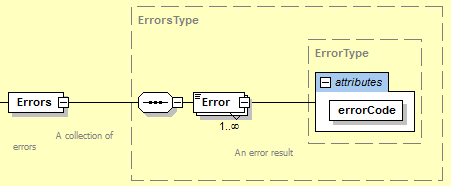
\includegraphics[width=1.0\textwidth]{figures/errors-schema-diagram.png}
  \caption{Errors Schema Diagram}
  \label{fig:errors-schema-diagram}
\end{figure}

\FloatBarrier

\tabulinesep = 5pt
\begin{longtabu} to \textwidth {
    |l|X[3l]|X[0.75l]|}
\caption{MTConnect Errors Element} \label{table:mtconnect-errors-element} \\

\hline
Element & Description & Occurrence \\
\hline
\endfirsthead

\hline
\multicolumn{3}{|c|}{Continuation of Table \ref{table:mtconnect-errors-element}}\\
\hline
Element & Description & Occurrence \\
\hline
\endhead

\gls{errors}	
&
An \gls{xml} container element in an \gls{mtconnecterrors response document} provided by an \gls{agent} when an error is encountered associated with a \gls{request} for information from a client software application.
\newline There \MUST be only one \gls{errors} element in an \gls{mtconnecterrors response document}.
\newline The \gls{errors} element \MUST contain at least one \gls{error} \gls{data entity} element.
&
1 \\
\hline


\end{longtabu}

\begin{note}
Note:	When compatibility with Version 1.0.1 and earlier of the MTConnect Standard is required for an implementation, the \gls{mtconnecterrors response document} contains only a single \gls{error} \gls{data entity} and the \gls{errors} \gls{structural element} \MUSTNOT appear in the document. 

\end{note}

\clearpage

\subsubsection{Error Data Entity}

When an \gls{agent} encounters an error when responding to a \gls{request} for information from a client software application, the information describing the error(s) is reported as a \gls{data entity} in an \gls{mtconnecterrors response document}.   \glspl{data entity} are organized in the \gls{errors} \gls{xml} container.

There is only one type of \gls{data entity} defined for an \gls{mtconnecterrors response document}.  That \gls{data entity} is called \gls{error}.

The following is an illustration of the structure of an \gls{xml} document demonstrating how \gls{error} \glspl{data entity} are reported in an \gls{mtconnecterrors response document}:

\begin{lstlisting}[firstnumber=1,escapechar=|,%
caption={Example of Error in MTConnectError}, label={lst:error-in mtconnecterror}]
<MTConnectError}>
  <Header/>
  <Errors>
    <Error/>
    <Error/>
    <Error/>
  </Errors>
</MTConnectError}>    
\end{lstlisting}

The \gls{errors} element \MUST contain at least one \gls{data entity}.  Each \gls{data entity} describes the details for a specific error reported by an \gls{agent} and is represented by the \gls{xml} element named \gls{error}.

\gls{error} \gls{xml} elements \MAY contain both attributes and \gls{cdata} that provide details further defining a specific error.  The \gls{cdata} \MAY provide the complete text provided by an \gls{agent} for the specific error.  

\paragraph{XML Schema Structure for Error}\mbox{}

The \gls{xml schema} in \fig{error-schema-diagram} represents the structure of an \gls{error} \gls{xml} element showing the attributes defined for \gls{error}.

\begin{figure}[ht]
  \centering
  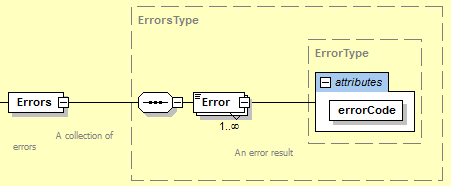
\includegraphics[width=0.75\textwidth]{figures/error-schema-diagram.png}
  \caption{Error Schema Diagram}
  \label{fig:error-schema-diagram}
\end{figure}

\FloatBarrier

\paragraph{Attributes for Error}\mbox{}

\gls{error} has one attribute.  \tbl{attributes-for-error} defines this attribute that provides additional information for an \gls{error} \gls{xml} element.   

\tabulinesep = 5pt
\begin{longtabu} to \textwidth {
    |l|X[3l]|X[0.75l]|}
\caption{Attributes for Error} \label{table:attributes-for-error} \\

\hline
Attribute & Description & Occurrence \\
\hline
\endfirsthead

\hline
\multicolumn{3}{|c|}{Continuation of Table \ref{table:attributes-for-error}}\\
\hline
Attribute & Description & Occurrence \\
\hline
\endhead

\gls{errorcode}
&
Provides a descriptive code that indicates the type of error that was encountered by an \gls{agent} when attempting to respond to a \gls{request} for information.
\newline \gls{errorcode} is a required attribute.
&
1 \\
\hline


\end{longtabu}

\paragraph{Values for errorCode}\mbox{}

There is a limited vocabulary defined for \gls{errorcode}.  The value returned for \gls{errorcode} \MUST be one of the following:

\newpage

\tabulinesep = 5pt
\begin{longtabu} to \textwidth {
    |l|X[3l]|}
\caption{Values for errorCode} \label{table:values-for-errorcode} \\

\hline
Value for errorCode & Description \\
\hline
\endfirsthead

\hline
\multicolumn{2}{|c|}{Continuation of Table \ref{table:values-for-errorcode}}\\
\hline
Value for errorCode & Description \\
\hline
\endhead

\gls{assetnotfound value}
&
The \gls{request} for information specifies an \gls{mtconnect asset} that is not recognized by the \gls{agent}.
\\ \hline

\gls{internalerror value}
&
The \gls{agent} experienced an error while attempting to published the requested information. 
\\ \hline


\gls{invalidrequest value}
&
The \gls{request} contains information that was not recognized by the \gls{agent}.
\\ \hline

\gls{invaliduri value}
&
The URI provided was incorrect. 
\\ \hline

\gls{invalidxpath value}
&
The \gls{xpath} identified in the \gls{request} for information could not be parsed correctly by the \gls{agent}.  This could be caused by an invalid syntax or the \gls{xpath} did not match a valid identify for any information stored in the \gls{agent}. 
\\ \hline

\gls{nodevice value}
&
The identity of the piece of equipment specified in the \gls{request} for information is not associated with the \gls{agent}.
\\ \hline

\gls{outofrange value}
&
The \gls{request} for information specifies \gls{streaming data} that includes sequence number(s) for pieces of data that are beyond the end of the \gls{buffer}.
\\ \hline

\gls{queryerror value}
&
The \gls{agent} was unable to interpret the \gls{query}.  The \gls{query} parameters do not contain valid values or include an invalid parameter.
\\ \hline

\gls{toomany value}
&
The \gls{count model} parameter provided in the \gls{request} for information requires either of the following:
\newline \tab- \gls{streaming data} that includes more pieces of data than the \gls{agent} is capable of organizing in an \gls{mtconnectstreams response document}. 
\newline \tab- Assets that include more \glspl{asset document} in an \gls{mtconnectassets response document} than the \gls{agent} is capable of handling. 
\\ \hline

\gls{unauthorized value}
&
The \gls{requester} does not have sufficient permissions to access the requested information.
\\ \hline

\gls{unsupported value}
&
A valid \gls{request} was provided, but the \gls{agent} does not support the feature or type of \gls{request}.
\\ \hline

\end{longtabu}

\paragraph{CDATA for Error}\mbox{}

The \gls{cdata} for \gls{error} contains a textual description of the error and any additional information an \gls{agent} is capable of providing regarding a specific error.  The \gls{valid data value} returned for \gls{error} \MAY be any text string.

\subsubsection{Examples for MTConnectError}

\lst{structure-for-mtconnecterror} is an example demonstrating the structure of an \gls{mtconnecterrors response document}:

\begin{lstlisting}[firstnumber=1,escapechar=|,% 
caption={Example of structure for MTConnectError}, label={lst:structure-for-mtconnecterror}]
<?xml version="1.0" encoding="UTF-8"?>
  <MTConnectError
  xmlns="urn:mtconnect.org:MTConnectError:1.4"
  xmlns:xsi=http://www.w3.org/2001/XMLSchema-instance
  xsi:schemaLocation="urn:mtconnect.org:MTConnectError
    :1.4/schemas/MTConnectError_1.4.xsd">
  <Header creationTime="2010-03-12T12:33:01Z"
    sender="MyAgent" version="1.4.1.10" 
    bufferSize="131000" instanceId="1383839" />
  <Errors>
    <Error errorCode="OUT_OF_RANGE" >Argument was 
      out of range</Error>
    <Error errorCode="INVALID_XPATH" >Bad 
      path</Error>
  </Errors>
</MTConnectError>
\end{lstlisting}

\lst{structure-for-mtconnecterror-when-backward-compatibility-is-required} is an example demonstrating the structure of an \gls{mtconnecterrors response document} when backward compatibility with Version 1.0.1 and earlier of the MTConnect Standard is required.  In this case, the \gls{document body} contains only a single \gls{error} \gls{data entity} and the \gls{errors} \gls{structural element} \MUSTNOT appear in the document. 

\begin{lstlisting}[firstnumber=1,escapechar=|,% 
caption={Example of structure for MTConnectError when backward compatibility is required}, label={lst:structure-for-mtconnecterror-when-backward-compatibility-is-required}]
<?xml version="1.0" encoding="UTF-8"?>
<MTConnectError
  xmlns="urn:mtconnect.org:MTConnectError:1.1"
  xmlns:xsi=http://www.w3.org/2001/XMLSchema-instance
  xsi:schemaLocation="urn:mtconnect.org:MTConnectError
    :1.1/schemas/MTConnectError_1.1.xsd">
  <Header creationTime="2010-03-12T12:33:01Z"
    sender="MyAgent" version="1.1.0.10" 
    bufferSize="131000" instanceId="1383839" />
  <Error errorCode="OUT_OF_RANGE" >Argument was out 
    of range</Error>
</MTConnectError>
\end{lstlisting}




\appendix
\section*{Appendices}
\addcontentsline{toc}{section}{Appendices}
\renewcommand{\thesubsection}{\Alph{subsection}}

\subsection{Bibliography}
\label{Bibliography}

Engineering Industries Association. \textit{EIA Standard - EIA-274-D}, Interchangeable Variable, Block Data Format for Positioning, Contouring, and Contouring/Positioning Numerically Controlled Machines. Washington, D.C. 1979.

ISO TC 184/SC4/WG3 N1089. \textit{ISO/DIS 10303-238:} Industrial automation systems and integration  Product data representation and exchange  Part 238: Application Protocols: Application interpreted model for computerized numerical controllers. Geneva, Switzerland, 2004.

International Organization for Standardization. \textit{ISO 14649:} Industrial automation systems and integration - Physical device control - Data model for computerized numerical controllers - Part 10: General process data. Geneva, Switzerland, 2004.

International Organization for Standardization. \textit{ISO 14649:} Industrial automation systems and integration - Physical device control - Data model for computerized numerical controllers - Part 11: Process data for milling. Geneva, Switzerland, 2000.

International Organization for Standardization. \textit{ISO 6983/1} - Numerical Control of machines - Program format and definition of address words - Part 1: Data format for positioning, line and contouring control systems. Geneva, Switzerland, 1982.

Electronic Industries Association. \textit{ANSI/EIA-494-B-1992}, 32 Bit Binary CL (BCL) and 7 Bit ASCII CL (ACL) Exchange Input Format for Numerically Controlled Machines. Washington, D.C. 1992.

National Aerospace Standard. \textit{Uniform Cutting Tests} - NAS Series: Metal Cutting Equipment Specifications. Washington, D.C. 1969.

International Organization for Standardization. \textit{ISO 10303-11:} 1994, Industrial automation systems and integration  Product data representation and exchange  Part 11: Description methods: The EXPRESS language reference manual. Geneva, Switzerland, 1994.

International Organization for Standardization. \textit{ISO 10303-21:} 1996, Industrial automation systems and integration -- Product data representation and exchange -- Part 21: Implementation methods: Clear text encoding of the exchange structure. Geneva, Switzerland, 1996.

H.L. Horton, F.D. Jones, and E. Oberg. \textit{Machinery's Handbook}. Industrial Press, Inc. New York, 1984.

International Organization for Standardization. \textit{ISO 841-2001:} Industrial automation systems and integration - Numerical control of machines - Coordinate systems and motion nomenclature. Geneva, Switzerland, 2001.

\textit{ASME B5.59-2 Version 9c: Data Specification for Properties of Machine Tools for Milling and Turning. 2005.}

\textit{ASME/ANSI B5.54: Methods for Performance Evaluation of Computer Numerically Controlled Lathes and Turning Centers. 2005.}

OPC Foundation. \textit{OPC Unified Architecture Specification, Part 1: Concepts Version 1.00. July 28, 2006.}

View the following site for RFC references: http://www.faqs.org/rfcs/.

\pagebreak

\subsection{Fundamentals of Using XML to Encode Response Documents}
\label{appendix:A}

The MTConnect Standard specifies the structures and constructs that are used to encode \glspl{response document}.  When these \glspl{response document} are encoded using XML, there are additional rules defined by the XML standard that apply for creating an XML compliant document.  An implementer should refer to the W3C website for additional information on XML documentation and implementation details - http://www.w3.org/XML.

The following provides specific terms and guidelines referenced in the MTConnect Standard for forming \glspl{response document} with XML:  

\begin{itemize}
\item \cfont{tag}:  A \cfont{tag} is an XML construct that forms the foundation for an XML expression.  It defines the scope (beginning and end) of an XML expression.  The main types of tags are: 

\item \cfont{start-tag}:  Designates the beginning on an XML element; e.g., <\gls{element name}> 

\item \cfont{end-tag}:  Designates the end on an XML element; e.g., </\gls{element name}>. 

\begin{note}
Note: If an element has no \glspl{child element} or \gls{cdata}, the \cfont{end-tag} may be shortened to />.
\end{note}

\item \cfont{Element}:  An element is an XML statement that is the primary building block for a document encoded using XML.  An element begins with a \cfont{start-tag} and ends with a matching \cfont{end-tag}.  The characters between the \cfont{start-tag} and the \cfont{end-tag} are the element's content.  The content may contain attributes, \gls{cdata}, and/or other elements.  If the content contains additional elements, these elements are called \glspl{child element}.

An example would be:  <\gls{element name}>Content of the Element</\gls{element name}>.

\item \gls{child element}:  An XML element that is contained within a higher-level \gls{parent element}.  A \gls{child element} is also known as a sub-element.  XML allows an unlimited hierarchy of \gls{parent element}-\gls{child element} relationships that establishes the structure that defines how the various pieces of information in the document relate to each other.  A \gls{parent element} may have multiple associated \glspl{child element}.

\item \gls{element name}:  A descriptive identifier contained in both the \cfont{start-tag} and \cfont{end-tag} that provides the name of an XML element.

\item \cfont{Attribute}:  A construct consisting of a name-value pair that provides additional information about that XML element.  The format for an attribute is \cfont{name="value"}; where the value for the attribute is enclosed in a set of quotation (") marks.  An XML attribute \MUST only have a single value and each attribute can appear at most once in each element.  Also, each attribute \MUST be defined in a \gls{schema} to either be required or optional.   

\item An example of attributes for an XML element is \lst{attributes-for-an-element}:

\begin{lstlisting}[firstnumber=1,escapechar=|,%
    caption={Example of  attributes for an element}, label={lst:attributes-for-an-element}]
<DataItem category="SAMPLE" id="S1load"
  nativeUnits="PERCENT"  type="LOAD"
  units="PERCENT"/>
\end{lstlisting}

In this example, \gls{dataitem} is the \gls{elementname}.  \gls{category}, \gls{id}, \gls{nativeunits}, \gls{type}, and \gls{units} are the names of the attributes.  "\gls{sample category}", "\cfont{S1load}", "\gls{percent}", "\gls{load sample}", and "\gls{percent}" are the values for each of the respective attributes.

\item \gls{cdata}:  \gls{cdata} is an XML term representing \textit{Character Data}. \textit{Character Data} contains a value(s) or text that is associated with an XML element.  \gls{cdata} can be restricted to certain formats, patterns, or words.  

An example of \gls{cdata} associated with an XML element would be \lst{cdata-associated-with-element}:

\begin{lstlisting}[firstnumber=1,escapechar=|,%
    caption={Example of cdata associated with element}, label={lst:cdata-associated-with-element}]
<Message id="M1">This is some text</Message>
\end{lstlisting}

In this example, \glselementname{message event} is the \gls{elementname} and \cfont{This is some text} is the \gls{cdata}.

\item \gls{namespace}:  An XML \gls{namespace} defines a unique vocabulary for named elements and attributes in an XML document.  An XML document may contain content that is associated with multiple \glspl{namespace}.  Each \gls{namespace} has its own unique identifier. 

Elements and attributes are associated with a specific \gls{namespace} by placing a prefix on the name of the element or attribute that associates that name to a specific \gls{namespace}; e.g., \cfont{x:MyTarget} associates the element name \cfont{MyTarget} with the \gls{namespace} designated by \cfont{x:} (the prefix).

\glspl{namespace} are used to avoid naming conflicts within an XML document.  The naming convention used for elements and attributes may be associated with either the default \gls{namespace} specified in the \gls{header term} of an XML document or they may be associated with one or more alternate \glspl{namespace}.  All elements or attributes associated with a \gls{namespace} that is not the default \gls{namespace}, must include a prefix (e.g., x:) as part of the name of the element or attribute to associate it with the proper \gls{namespace}.  See \apx{Schema and Namespace Declaration Information} for details on the structure for XML \glspl{header term}.

The names of the elements and attributes declared in a \gls{namespace} may be identified with a different prefix than the prefix that signifies that specific \gls{namespace}.  These prefixes are called \gls{namespace} aliases.  As an example, MTConnect Standard specific \glspl{namespace} are designated as \cfont{m:} and the names of the elements and attributes defined in that \gls{namespace} have an alias prefix of \cfont{mt:} which designates these names as MTConnect Standard specific vocabulary; e.g., \cfont{mt:MTConnectDevices}. 
\end{itemize}

XML documents are encoded with a hierarchy of elements.  In general, XML elements may contain \glspl{child element}, \gls{cdata}, or both.  However, in the MTConnect Standard, an element \MUSTNOT contain mixed content; meaning it cannot contain both \glspl{child element} and \gls{cdata}. 

The \gls{semantic data model} defined for each \gls{response document} specifies the elements and \glspl{child element} that may appear in a document.  The \gls{semantic data model} also defines the number of times each element and \gls{child element} may appear in the document.

\lst{hierarchy-of-xml-elements} demonstrates the hierarchy of XML elements and \glspl{child element} used to form an XML document:

\begin{lstlisting}[firstnumber=1,escapechar=|,%
    caption={Example of hierarchy of XML elements}, label={lst:hierarchy-of-xml-elements}]
<Root Level>    (Parent Element)
  <First Level>  (Child Element to Root Level and 
  Parent Element to Second Level)
    <Second Level>  (Child Element to First Level
    and Parent Element to Third Level)
      <Third Level name="N1"></Third Level>  
      (Child Element to Second Level)
      <Third Level name="N2"></Third Level>  
      (Child Element to Second Level)
      <Third Level name="N3"></Third Level>  
      (Child Element to Second Level)
    </Second Level>   (end-tag for Second Level)
  </First Level>   (end-tag for First Level)
</Root Level>   (end-tag for Root Level)
\end{lstlisting}


In the \lst{hierarchy-of-xml-elements}, \textit{Root Level} and \textit{First Level} have one \gls{child element} (sub-elements) each and Second Level has three \glspl{child element}; each called \textit{Third Level}.  Each \textit{Third Level} element has a different name attribute.  Each level in the structure is an element and each lower level element is a \gls{child element}.

\pagebreak

\subsection{Schema and Namespace Declaration Information}
\label{appendix:Schema and Namespace Declaration Information}

There are four pseudo-attributes typically included in the \gls{header term} of a \gls{response document} that declare the \gls{schema} and \gls{namespace} for the document.  Each of these pseudo-attributes provides specific information for a client software application to properly interpret the content of the \gls{response document}.

The pseudo-attributes include:

\begin{itemize}

\item \cfont{xmlns:xsi} - The \cfont{xsi} portion of this attribute name stands for \gls{xml schema} instance.  An \gls{xml schema} instance provides information that may be used by a software application to interpret XML specific information within a document.  See the W3C website for more details on \cfont{xmlns:xsi}.

\item \cfont{xmlns} - Declares the default \gls{namespace} associated with the content of the \gls{response document}.  The default \gls{namespace} is considered to apply to all elements and attributes whenever the name of the element or attribute does not contain a prefix identifying an alternate \gls{namespace}.

The value of this attribute is an URN identifying the name of the file that defines the details of the \gls{namespace} content.  This URN provides a unique identify for the \gls{namespace}.

\item \cfont{xmlns:m} - Declares the MTConnect specific \gls{namespace} associated with the content of the \gls{response document}.  There may be multiple \glspl{namespace} declared for an XML document.  Each may be associated to the default \gls{namespace} or it may be totally independent.  The \cfont{:m} designates that this is a specific MTConnect \gls{namespace} which is directly associated with the default \gls{namespace}.

\begin{note} 
Note:	See \sect{Extensibility} for details regarding extended \glspl{namespace}.
\end{note}

The value associated with this attribute is an URN identifying the name of the file that defines the details of the \gls{namespace} content.

\item \cfont{xsi:schemaLocation} -  Declares the name for the \gls{schema} associated with the \gls{response document} and the location of the file that contains the details of the \gls{schema} for that document.

The value associated with this attribute has two parts:

\tab - A URN identifying the name of the specific \gls{xml schema} instance associated with the \gls{response document}.

\tab - The path to the location where the file describing the specific \gls{xml schema} instance is located.  If the file is located in the same root directory where the \gls{agent} is installed, then the local path MAY be declared.  Otherwise, a fully qualified URL must be declared to identify the location of the file.

\begin{note}
Note:	In the format of the value associated with \cfont{xsi:schemaLocation}, the URN and the path to the \gls{schema} file \MUST be separated by a "space".
\end{note}

\end{itemize}

In \lst{schema-and-namespace-declaration}, the first line is the \gls{xml declaration}.  The second line is a \gls{root element} called \gls{mtconnectdevices}.  The remaining four lines are the pseudo-attributes of \gls{mtconnectdevices} that declare the XML \gls{schema} and \gls{namespace} associated with an \gls{mtconnectdevices response document}.

\begin{lstlisting}[firstnumber=1,escapechar=|,%
    caption={Example of schema and namespace declaration}, label={lst:schema-and-namespace-declaration}]
<?xml version="1.0" encoding="UTF-8"?>
  <MTConnectDevices
   xmlns:xsi=http://www.w3.org/2001/XMLSchema-instance
   xmlns="urn:mtconnect.org:MTConnectDevices:1.3"
   xmlns:m="urn:mtconnect.org:MTConnectDevices:1.3"
   xsi:schemaLocation="urn:mtconnect.org:
    MTConnectDevices:1.3 /schemas/MTConnectDevices\_1.3.xsd">
\end{lstlisting}

The format for the values provided for each of the pseudo-attributes \MUST reference the \gls{semantic data model} (e.g., \gls{mtconnectdevices}, \gls{mtconnectstreams}, \gls{mtconnectassets}, or \gls{mtconnecterror}) and the version (i.e.; \cfont{1.1, 1.2, 1.3}, etc.) of the MTConnect Standard that depict the \gls{schema} and \gls{namespace}(s) associated with a specific \gls{response document}.

When an implementer chooses to extend an MTConnect \gls{data model} by adding custom data types or additional \glspl{structural element}, the \gls{schema} and \gls{namespace} for that \gls{data model} should be updated to reflect the additional content.  When this is done, the \gls{namespace} and \gls{schema} information in the \gls{header term} should be updated to reflect the URI for the extended \gls{namespace} and \gls{schema}. 




\end{document}
